

\documentclass[11pt,a4paper,titlepage]{report}
% a4paper : format papier
% one side : impression recto vs. twoside : recto-verso

% ----------------------------------------------------------------------
% CHARGEMENT DES PACKAGES
% ----------------------------------------------------------------------

%------ Language
\usepackage[francais,english]{babel} %langue du doc = 2eme ecrite
								 	 %\selectlanguage{nom-de-la-langue} 										  pour doc bilingue
\usepackage[utf8]{inputenc} %package accents (ou latin1 à la place de 									utf8)
\usepackage[T1]{fontenc}    %package accents

\usepackage{lscape}         %for landscape pages 
%------ Math
\usepackage{amssymb,amsfonts,amsmath} 		% Caracteres math.

%------ Mise en forme
%\usepackage{fancyhdr} 		% Modifier les en-tete et co 
%\usepackage{type1cm}		% Permet d'utilisr des tailles arbitraires de police

%------ Color
\usepackage{color}			% Colorer un texte
\usepackage[table]{xcolor}	% Extension du package color (options table pour + de couleurs possibles)
\usepackage{colortbl} 		% Colorer les cellules d'un tableau

%------ Image et insertion
\usepackage{graphicx}		% Insertion d'image
\usepackage{subfigure}		% Insertion de sous-figures
\usepackage{pdfpages}		% Insertion de ficher .pdf mais produit un DVI

%------ Caracteres speciaux
\usepackage{pifont}			% Caractères ding
\usepackage{lettrine}		% Lettrine
\usepackage{eurosym} 		% \euro Insertion du symbole euro


\usepackage{hyperref}		%\url{} pour envoyer vers site
							%\href{http://www.truc.org}{mot} mot servant 								de lien
							%\href{mailto:truc@bidon.org}{truc@bidon.org} 							lien mail to
							
\usepackage{multirow}							
%------ Presentation d'algorithme
%\usepackage{algorithmic}			% Algorithme
%\usepackage[chapter]{algorithm}		% Algorithme sous forme de flottants (avec numerotation de chapitre)

%------ Notes to do
\usepackage{todonotes}

%----- Divers
%\usepackage{ifthen}						% Structures de programmation (if, while,...)
%\usepackage{environ}					% Definition des nouveaux environnements

\usepackage{titlesec}

\titleclass{\subsubsubsection}{straight}[\subsection]

\newcounter{subsubsubsection}[subsubsection]
\renewcommand\thesubsubsubsection{\thesubsubsection.\arabic{subsubsubsection}}
\renewcommand\theparagraph{\thesubsubsubsection.\arabic{paragraph}} % optional; useful if paragraphs are to be numbered

\titleformat{\subsubsubsection}
  {\normalfont\normalsize\bfseries}{\thesubsubsubsection}{1em}{}
\titlespacing*{\subsubsubsection}
{0pt}{3.25ex plus 1ex minus .2ex}{1.5ex plus .2ex}

\makeatletter
\renewcommand\paragraph{\@startsection{paragraph}{5}{\z@}%
  {3.25ex \@plus1ex \@minus.2ex}%
  {-1em}%
  {\normalfont\normalsize\bfseries}}
\renewcommand\subparagraph{\@startsection{subparagraph}{6}{\parindent}%
  {3.25ex \@plus1ex \@minus .2ex}%
  {-1em}%
  {\normalfont\normalsize\bfseries}}
\def\toclevel@subsubsubsection{4}
\def\toclevel@paragraph{5}
\def\toclevel@paragraph{6}
\def\l@subsubsubsection{\@dottedtocline{4}{7em}{4em}}
\def\l@paragraph{\@dottedtocline{5}{10em}{5em}}
\def\l@subparagraph{\@dottedtocline{6}{14em}{6em}}
\makeatother

\setcounter{secnumdepth}{4}
\setcounter{tocdepth}{4}

\def\doubleunderline#1{\underline{\underline{#1}}}
% ----------------------------------------------------------------------
% DEFINITION DU FORMAT (A4 = 21 x 29.7 cm)
% ----------------------------------------------------------------------

% - Simplified definition
\usepackage[top=2.2cm, bottom=2.2cm, left=2.5cm, right=2.5cm]{geometry}

% - Detailled definition
%% Set an additionnal left margin - The default is 1 inch (2.54cm), so the following
%% command sets a 3cm left margin.
%\setlength{\oddsidemargin}{0.46cm} 		% Pour les pages impaires (so: 3 cm)
%\setlength{\evensidemargin}{-0.54cm} 	% Pour les pages paires if recto-verso printing is used (so: 2 cm)
%
%% Set width of the text - What is left will be the right margin.
%\setlength{\textwidth}{16.0cm} 			% (so : 2 cm)
%
%% Set an additionnal top margin - The default is 1 inch (2.54cm)
%\setlength{\topmargin}{-1.04cm} 		% (so 1.5 cm)
%
%% Set height of the text - What is left will be the bottom margin.
%% In this case, bottom margin is 29.7cm -1.5cm -26.7cm = 29.7cm - 28.2cm = 1.5cm
%\setlength{\textheight}{26.7cm}

% - Header and footer parameters
%\setlength{\headsep}{1.0cm} Set vertical distance between the header and the text
%\setlength{\headsep}{0.5cm}

% Set vertical distance between the last text line and the
% firts line of the bottom of footer
%\setlength{\footskip}{1.0cm}

% Set paragraph spacing parameter
%\setlength{\parskip}{0.5cm} 		% set l'espace entre deux paragraphes, avec les titres,...
%\setlength{\parindent}{0.0cm} 		% definit la valeur de l'alinea (15 pt par defaut)

%\def\baselinestretch{1.0} 	% permet de gérer l'interlignage

%\widowpenalty=10000 		% empeche au maximum la coupure de paragraphe avant la derniere ligne (pas de ligne isolée à la page suivante)
%\clubpenalty=10000     	% empeche au maximum la coupure de paragraphe apres la premiere ligne (pas de ligne orpheline en bas de page)
%\raggedbottom           	% empeche l'etirement des ressorts verticaux (mais peut creer des variations de hauteur de texte importantes, surtout avec les 2 commandes ci-dessus !)

% Hearder and footer. By default, the document contains only the page numerotation.
%\pagestyle{empty} 			% Delete the page number (header + footer = empty)
%\pagestyle{fancy}			% Insert header and footer
%\lhead{haut de page a gauche}
%\chead{haut de page au centre}
%\rhead{haut de page a droite}
%\lfoot{pied de page a gauche}
%\cfoot{pied de page au centre}
%\rfoot{pied de page a droite}
%\renewcommand{\headrulewidth}{0.0pt} 				% Suppression de la ligne de page supérieure

%\fancyhead[RO,RE]{\thepage}						% Commandes pour document recto-verso (twoside)
%\fancyhead[LO,LE]{}
%\fancyfoot{}

% ==============================================================
\begin{document}

% ----------------------------------------------------------------------
% COMMANDES UTILES	
% ----------------------------------------------------------------------
% -Inserer une table des matieres ou autres tables
% \tableofcontents
% \listoffigures
% \listoftables
% \setcounter{tocdepth}{2} %définit la "profondeur" de la table des matières...
%
% -Inserer une nouvelle page
% \newpage
%
% -Inserer un nouveau chapitre sans numero mais present dans la table des mat
% \chapter*{Introduction}
% \addcontentsline{toc}{chapter}{Introduction}
%
% -Renommer le nom d'un chapitre
% \renewcommand{\chaptername}{Partie}
%
% -Forcer la valeur d'un compteur (ici de page):
% 	\setcounter{page}{1}
%		 
% -Inclure un fichier pdf
% 	\includepdf[pages=-]{cover_book_page.pdf}
%
% -Inserer une image en flottant + légende + label 
% 	\begin{figure}
% 		\begin{center}
% 		\includegraphics[scale=0.5]{Filename.jpg}
% 		\caption{Legende}
% 		\label{Label pour la figure}
% 		\end{center}
% 	\end{figure}
%
% -Idem mais avec sous-figure
% \begin{figure}
%  \centering
%    \subfigure[]{\label{Label pour la figure} \includegraphics[scale=0.35]{Filename.jpg}}
%    \subfigure[]{\label{Label pour la figure} \includegraphics[scale=0.35]{Filename.jpg}}
%	\caption{Legende}
% \end{figure}
%
% -Barrière pour flottants
% \FloatBarrier




%--------------------------------
%-----Page de garde -------------
%--------------------------------
% use word => convert to pdf => insert it
% Old version:
%
%\begin{titlepage}
%
%\begin{figure}
%	\begin{minipage}[h]{0.16\linewidth}
%	\begin{center}
%		\includegraphics[height=1.8cm]{Images/Logo_Ulg.jpg}
%	\end{center}
%	\end{minipage} \hfill
%	\begin{minipage}[h]{0.69\linewidth}
%	\begin{center}
%		{\Large Université de Liège \\
%				Faculté des Sciences Appliquées \\
%				Année Académique 2013-2014\\}
%	\end{center}
%	\end{minipage} 
%	\begin{minipage}[h]{0.13\linewidth}
%	\begin{center}
%		\includegraphics[width=3.5cm]{Images/Logo_LTAS.jpg}
%%		\includegraphics[width=3.5cm]{Images/Logo_fsa.jpg}
%	\end{center}
%	\end{minipage}   
%\end{figure}
%
%\vspace*{3cm}
%
%\begin{center}
%	{\Large \textbf{MECA0029-1 : } Théorie des vibrations\\}
%	\vspace{0.1cm}	
%	{\Large J-C. Golinval\\}
%	\vspace{3 cm}
%
%	{\huge Analyse du comportement dynamique d'une queue d'hélicoptère :\\}
%	\vspace{0.25cm}	
%	{\Huge Partie 1 : Modélisation de la structure}	
%	\rule{16cm}{0.5 pt}	
%\end{center}
%
%\vspace{7 cm}
%
%\begin{center}
%{\Large Julien \textsc{Leclerc} \\ Romain \textsc{Van Hulle}}
%\end{center}
%
%\end{titlepage}	


% ----------------------------------------------------------------------
% ----------------------------------------------------------------------
% DEBUT DU DOCUMENT	
% ----------------------------------------------------------------------
% ----------------------------------------------------------------------

%Page d'en tête
%Remerciements?

\begin{titlepage}
\begin{center}
\begin{figure}
    \centering
        \includegraphics[width=6cm]{logo_dtu.jpg}
\end{figure}
\ \\ 
Department of Civil Engineering\\
December 7th 2018\\
\end{center}
\begin{flushleft}
\vspace{3cm}
\begin{center}
\Huge
\textbf{11374 - Seismic \& Wind Engineering}\\
\textbf{Project Report}\\
\end{center}
\rule[0.5ex]{\textwidth}{0.1mm}
\end{flushleft}
\begin{flushleft}
\begin{center}
\LARGE{Group 2}
\end{center}

\end{flushleft}
\vfill

\begin{flushleft}
\begin{center}
\textnormal{Natalie Bennett - s181674}\\
\end{center}
\end{flushleft}

\end{titlepage}


\newpage
 \tableofcontents
\thispagestyle{empty}

\newpage
\setcounter{page}{1}

\chapter{Background Information}
\section{Introduction}
\paragraph{} With great power comes great responsibility. As civil engineers, we are obligated to design structures that prioritize the safety of the public above all. This includes the consideration of environmental forces derived from seismic or wind sources that may be imposed upon the structure. These environmental forces have the power to inflict damage on the structural and non-structural elements of a building. The damages result in significant economic losses and all too often also lead to the loss of life. As engineers, we are not fulfilling our duty to the public if through the design process, we do not sufficiently account for the effects attributed to these environmental hazards.
\paragraph{} When a fault ruptures within the Earth's subsurface it generates strong ground motions in the form of waves that travel through the Earth in the surrounding area. The media through which a wave propagates has the ability to amplify these ground motions, thereby inflicting greater damage on the structure. Thorough geological investigations are fundamental in order to properly conduct a structural seismic analysis. 
\paragraph{} The seismic analysis of a structure therefore considers the interaction of these ground motions with the structural elements of a building. This begins with understanding the dynamic characteristics of the building. The second stage of this assessment is to study the structural response of the building, this is determined through both the modal response spectrum analysis and the time history analyses. The next step in this assessment is the design verification of the building which is based on Eurocode 8. As the soil-structure interaction can have a detrimental influence on the seismic response of a structure, it will be subsequently presented in more detail as it is imperative that the analysis accounts for this relationship. 
\paragraph{}With the expected warming of our planet, the global climate is expected to undergo changes in the coming decades. The increase in temperature is expected to increase the intensity and frequency of storms around the world. Storms which will potentially exceed our norms \cite{Climate}. With this forecast it is more important than ever that as civil engineers we comprehend the effects of environmental phenomena, such as extreme winds, and how to design out structures to fulfill our duty of keeping the public safe. The wind part of this report is focused on wind statistics from real and wind tunnel data, and how to apply each to the other. This part looks at both a low rise and high rise structure 
\paragraph{}With this in mind, it is important to possess the competency and knowledge required to carry out the design of structures subjected to unique dynamic loading. With the objective of developing these, the aspects of structural analysis for earthquake and wind actions will be applied to both a low rise and high rise building.
\paragraph{}In the following, the specifications required to carry out the analyses will be addressed. The report is divided in two parts, with the first pertaining to the seismic engineering assessment and the later to the wind engineering assessment.
\newpage
\paragraph{Note to the Reader}
\begin{itemize}
    \item It should be noted that English conventions for the decimal and thousand separator have been used for the entirely of this report
\end{itemize}
\section{Specifications}
\paragraph{}This section contains all of the specifications for both the Seismic and Wind Engineering parts of the report. This includes the building specifications, material properties, soil properties, seismic data, and wind data. 
\begin{table}[h!]
  \begin{center}
    \begin{tabular}{c|c}
    \hline
      \textbf{Building Specifications}\\
      \hline
      Building Height, $H$ & $2.5\,[m]$\\
      Building Width, $W$ & $4.5\,[m]$\\
      Building Length, $L$ & $4.5\,[m]$\\
      Width of Column, $w_1$ & $0.4\,[m]$\\
      Length of Column, $d_1$ & $0.5\,[m]$\\
      Height of Beam, $h_{1}$ & $0.5\,[m]$\\
      Thickness of Beam, $t_{1}$ & $0.25\,[m]$\\
      Slab Thickness, $t_{sl}$ & $0.18\,[m]$\\
      Glass Thickness, $t_{gl}$ & $2\times5\,10^{-3}\,[m]$\\
      \hline
      \textbf{Vertical Loads}\\
      \hline
      Dead Load (first three stories), $G_1$ & $2.5\,[kN/m]$\\
      Dead Load (roof level), $G_2$ & $2.0\,[kN/m]$\\
      Live Load (first three stories), $Q_1$ & $4.0[kN/m]$\\
       \hline
       \textbf{Damping Properties}\\
         \hline
      Structural Damping, $\xi $ & $0.03\,[-]$\\
      Behavioral Factor, $q$ & $4.0\,[-]$ \\
       \end{tabular}
       \caption{Design Specifications - Low Rise Building - Seismic}
    \label{tab: Specifications - Design LowRB }
  \end{center}
\end{table}
\begin{table}[h!]
  \begin{center}
    \begin{tabular}{c|c}
    \hline
      \textbf{Building Specifications}\\
      \hline
      Building Height, $H$ & $102.0\,[m]$\\
      Building Width, $W$ & $48.6\, [m]$\\
      Building Depth, $D$ & $14.5\, [m]$\\
      Storey Height, $h_1$ & $3.0\, [m]$\\
      Thickness of RC Core, $t_c$ & $0.15\, [m]$ \\
      Width of RC Core, $W_C$ & $19\, [m]$\\
      Depth of RC Core, $D_C$ & $14.0\, [m]$\\
      Glass Thickness, $t_{gl}$ & $2\times5\,10^{-3}\,[m]$\\
      \hline
       \textbf{Vertical Loads}\\
      \hline
        Dead Load, $G$ & $8.1\,[kN/m]$\\
        Live Load, $Q$ & $2.0\,[kN/m]$\\
       \hline
       \textbf{Damping Properties}\\
         \hline
          Structural Damping, $\xi$ & $0.012\,[-]$\\
          Behavioral Factor, $q$ & $1.0\,[-]$
    \end{tabular}
     \caption{Design Specifications - High Rise Building - Seismic}
    \label{tab: Specifications - Design HighRB}
  \end{center}
\end{table}
\begin{table}[h!]
  \begin{center}
    \begin{tabular}{c|c}
    \hline
      \textbf{Material Properties}\\
      \hline
      Young's Modulus for Concrete, $E_c$ & $3.4\times10^{10}\,[N/m^2]$\\
      Density of Concrete, $\rho_{c}$ & $2400\,[kg/m^3]$ \\
      Concrete Grade & C25/30\\
      Steel Grade & C\\
      $f_{yk}$ & $500\,[MPa]$\\
      Density of Glass, $\rho_{gl}$ & $2600\,[kg/m^3]$ \\
       \end{tabular}
       \caption{Material Properties for High Rise and Low Rise Buildings}
    \label{tab: specifications - material properties}
  \end{center}
\end{table}
\begin{table}[h!]
  \begin{center}
    \begin{tabular}{c|c}
    \hline
      \textbf{Seismic Data}\\
      \hline
      Importance Class & II\\
      Importance Factor, $\gamma$ & $1.0\,[-]$\\
      Ground Acceleration, $a_g$ & $0.15g\,[m/s^2]$\\
      Soil Factor, S & $1.35\,[-]$\\
      Period B, $T_B$ & $0.2\,[s]$\\
      Period C, $T_C$ & $0.8\, [s]$\\
      Period D, $T_D$ & $2.0\, [s]$\\
      Cut Off Constant, $\beta$ & $0.2\,[-]$\\
      \end{tabular}
  \end{center}
   \caption{Seismic Specifications}
    \label{tab: specifications - seismic}
\end{table}
\begin{table}[h!]
  \begin{center}
    \begin{tabular}{c|c}
    \hline
      \textbf{Soil Specifications}\\
      \hline
      Soil Type & D\\
      Shear Wave Velocity & $160\,[m/s]$\\
      Density, $\rho_s$ & $1.7\,[tn/m^3]$\\
      Soil Thickness & $23\,[m]$\\
      Poisson's Ratio, $\nu$ & $0.3\,[-]$\\
      Soil Material Damping, $\xi_s$ & $0.05\,[-]$\\
      \end{tabular}
  \end{center}
  \caption{Soil Data}
    \label{tab: specifications - soil}
\end{table}
\begin{table}[h!]
    \centering
    \begin{tabular}{c|c}
    \hline
       \textbf{Time $[years]$} & \textbf{Mean Wind Speed $[m/s]$} \\
        \hline
        $1$ & $18.48$ \\
        $2$ & $18.67$ \\
        $3$ & $17.96$ \\
        $4$ & $18.46$ \\
        $5$ & $19.10$ \\
        $6$ & $20.34$ \\
        $7$ & $18.44$ \\
        $8$ & $21.28$ \\
        $9$ & $21.84$ \\
        $10$ & $18.42$ \\
        $11$ & $18.55$ \\
        $12$ & $20.72$ \\
        $13$ & $18.52$ \\
        $14$ & $21.66$ \\
        $15$ & $19.21$ \\
        $16$ & $21.54$ \\
        $17$ & $20.16$ \\
        $18$ & $19.44$ \\
        $19$ & $19.71$ \\
        $20$ & $19.49$ \\
    \end{tabular}
    \caption{Wind Data: Mean Wind Velocities over a 20 year period}
    \label{tab:wind data}
\end{table}
\begin{table}[h]
    \centering
    \begin{tabular}{c|c}
    \hline
    \textbf{Building Specifications}  \\
        \hline
        Length, $L$ & $45 \,[m]$  \\
        Span, $s$ & $27.5 \,[m]$ \\
        Eaves Height, $h$ & $11 \,[m]$ \\
        Roof Pitch & $5\,[degrees]$ \\
        \hline
    \textbf{Terrain Specifications}  \\
        \hline
        Terrain Type & II \\
        Reference Height of Specific Terrain Type, $z_o$ & $0.05\,[m]$ \\
        Eurocode Terrain Reference Height, $z_{o,II}$ & $0.05\,[m]$ \\
    \end{tabular}
    \caption{Design Specifications - Low Rise Building - Wind}
    \label{tab:wind low rise}
\end{table}
\begin{table}[h]
    \centering
    \begin{tabular}{c|c}
    \hline
    \textbf{Building Specifications}  \\
        \hline
       Elasticity Modulus, $E$ & $3.7$x$10^{10}\, [N/m^2]$ \\
       Critical Damping Ratio, $\xi_s$ & $0.012\,[-]$ \\
       Moment of Inertia (X,Z), $I_{yy}$ & $483.76\,[m^4]$ \\
       Moment of Inertia (Y,Z), $I_{xx}$ & $483.00\,[m^4]$ \\
       Torsional Moment of Inertia, $I_{zz}$ & $465.00\,[m^4]$ \\
       Eigenfrequency (X,Z), $f_0$ & $0.58\, [Hz]$ \\
       Eigenfrequency (Y,Z), $f_0$ & $0.49 \,[Hz]$ \\
       Torsional Eigenfrequency, $f_0$ & $0.87\, [Hz]$ \\
    \end{tabular}
    \caption{Design Specifications - High Rise Building - Wind}
    \label{tab:wind high rise}
\end{table}
%\subsection{Eurocode 8} 
%Eurocode 8 was created by the European Commision to outline the practices for the seismic design of buildings in Europe. 
%\subsubsection{Importance Class}
%\paragraph{}Eurocode 8 specifies four different "importance classes" based on the importance of a building. These importance classes have coresponding importance factors that must be used during the seismic analysis of a structure. The code specifies that buildings of minor importance for public safety are of lowest importance and belong to importance class I. Ordinary buildings belong to importance class II. Importance class III is concered with buildings such as schools and assembly halls in which the seismic resistance is of greater importance to protect the lives of those inside during a potential seismic event. Finally, hospitals, fire stations, and power plants belong to the highest importance class, IV, which specifies that the integrity of these buildings is of utmost importance during a seismic event to ensure safety and protection of the population. The buildings being assessed in this project belongs to importance class II. 
% Insert reference?? Eurocode 8: Seismic Design of Buildings

\newpage
\part{SEISMIC ENGINEERING}
%\todo{Need to decided global or generalized and be consistent with one term instead of using both}

\chapter{The Eigenvalue Problem}
\paragraph{}As previously explained, when designing a building in an area of seismic activity it is necessary to perform a seismic assessment of the design. This process is divided into several stages. Before beginning the assessment, the dynamic characteristics of the building must be determined, as they govern the seismic response. This has been determined using the eigenvalue problem in which the mass and stiffness matrices are obtained.
\paragraph{}The dynamic characteristics (i.e. the natural frequencies and natural vibration modes) of a structure are determined by solving the equation governed by the spatial variable in the decoupled equation of the free vibration system. This is shown below in \textsc{Equation}\,\eqref{eqI.1:governing equation 1} for the discretized system and \textsc{Equation}\,\eqref{eqI.1:governing equation 2} for the continuous system. 
\begin{equation}
    (\doubleunderline{K}-\doubleunderline{M}\,\omega^2_m)\underline{\phi_m}=0
    \label{eqI.1:governing equation 1}
\end{equation}
\paragraph{}Where,
\begin{itemize}
\begin{small}
    \item $K$ is the generalized stiffness matrix of the discretized system $[N]$
    \item $M$ is the generalized mass matrix of the discretized system $[kg]$
    \item $\omega_m$ is the $m^{th}$ angular frequency vector $[rad/s]$
    \item $\phi_m$ is the $m^{th}$ modal shape relative to $\omega_m$ $[-]$
\end{small}
\end{itemize}
\begin{equation}
    (E\,I\,\phi(x)')''-\omega^2_m\,\bar{m}\,\phi_m^{(x)}=0
    \label{eqI.1:governing equation 2}
\end{equation}
\paragraph{}Where,
\begin{itemize}
\begin{small}
    \item $E$ is the Young's modulus of the continuous system given in \textsc{Table}\,\ref{tab: specifications - material properties} $[N/m^2]$
    \item $I$ is the interia of the continuous system relative to the global axis of the structure being studied. $[kg\,m^2]$
    \item $\omega_m$ is the $m^{th}$ angular frequency vector $[rad/s]$
    \item $\bar{m}$ is the mass per unit length of the continuous system $[kg/m]$
    \item $\phi_m(x)$ is the $m^{th}$ modal shape relative to $\dfrac{d}{dx}$ where $x$ is the local coordinate along the continuous system $[-]$
\end{small}
\end{itemize}
\paragraph{}In the following sections, the derivation of the terms within these equations will be detailed. This method is outlined for both the low rise and high rise buildings using both the discrete and the continuous systems, respectively.
\section{Low Rise Building}
\begin{figure} [h]
    \centering
    \includegraphics[width=14cm]{3D_structure.jpeg}
    \caption{3D structure of Low Rise Building}
    \label{fig:3D LR}
\end{figure}
\begin{figure} [h]
    \centering
    \includegraphics[width=10cm]{low_rise_dimensions.jpeg}
    \caption{Cross section of Low Rise Building}
    \label{fig:I.1 - cross section of low rise building}
\end{figure}
\paragraph{}The low rise building is a three-dimensional structure that can be seen in \textsc{Figure}\,\ref{fig:3D LR} with an accompanying cross section in \textsc{Figure}\,\ref{fig:I.1 - cross section of low rise building}. The two frames of the building are analyzed as discrete systems with 12 degrees of freedom (DOF) as shown in \textsc{Figure} \ref{fig: I.1 - DOF}. This figure (\ref{fig: I.1 - DOF}) also shows the numeration of the elements composing the structure, outlining the global axis and the local axis, and the local DOF for each element. The assumptions that have been made for this building are as follows, the three dimensional structure will be modelled as two separate two dimensional frames, one in each direction. This low rise building is an idealized linear structure with reinforced slabs that will be considered rigid diaphragms. The columns will carry only their own weight, and the height of the glass considered for each storey will be half the height of glass above and half the height of glass below, so that the last floor and foundation will only take half of the height of the glass (see \textsc{Figure} \ref{fig:Height of Glass Considered}). No live load will be considered on the last storey, as it is the roof. Finally, the building will be analyzed as a discrete system.
\begin{figure} [h]
    \centering
    \includegraphics[width=14cm]{Local_and_global_DOF.jpeg}
    \caption{Sketch of the 2D frame : Local and Global DOF}
    \label{fig: I.1 - DOF}
\end{figure}
\paragraph{}To solve the equation governed by the spatial variable in the decoupled equation of the vibration system for the discrete system, \textsc{Equation}\,\eqref{eqI.1:governing equation 1}, the generalized stiffness and mass matrices must be determined. The following sections will outline this process. 
\subsection{Stiffness Matrix}
\paragraph{}Before the generalized stiffness matrices can be determined, the moment of inertia of the beams and the columns in both the (X,Z) plane and (Y,Z) plane must be derived. \textsc{Equation}\,\ref{eq:I.1 - Low Rise - Interia of Columns} and \textsc{Equation}\,\ref{eq:I.1 - Low Rise - Interia of Beams} below provide the inertia denoted as $I_c$, and $I_b$ for the columns and beams, respectively.
\begin{equation}
I_c = 
\left\lbrace
\begin{array}{rl}
  \dfrac{d_1\,w_1^3}{12} & \,\,\,in\,(X,Z)\,plane\\
  \\
  \dfrac{w_1\,d_1^3}{12} & \,\,\,in\,(Y,Z)\,plane\\
\end{array}
\right.
 \label{eq:I.1 - Low Rise - Interia of Columns}
\end{equation}
\begin{equation}
    \begin{array}{rl}
    I_b = \dfrac{t_1\,h_1^3}{12} & \,\,\,in\,both\,(X,Z)\,and\,(Y,Z)\,planes\
    \end{array}
 \label{eq:I.1 - Low Rise - Interia of Beams}
\end{equation}
\paragraph{}Where,
\begin{itemize}
\begin{small}
    \item $d_1$ is the depth of the column given in \textsc{Table}\,\ref{tab: Specifications - Design LowRB } $[m]$
    \item $w_1$ is the width of the column given in \textsc{Table}\,\ref{tab: Specifications - Design LowRB } $[m]$
     \item $t_1$ is the width of the beam given in \textsc{Table}\,\ref{tab: Specifications - Design LowRB } $[m]$
    \item $h_1$ is the height of the beam given in \textsc{Table}\,\ref{tab: Specifications - Design LowRB } $[m]$
\end{small}
\end{itemize}
\subsubsection{Local Stiffness Matrix}
\paragraph{}The generalized stiffness matrix is based on the combination of the component of the local stiffness matrix, $k$ $[N]$, of the element shown in \textsc{Figure}\,\ref{fig : I.1 - local axis LowRB}. Firstly, obtained through \textsc{Equation}\,\eqref{eq: I-1 local stiffness}, the local stiffness matrix of each element is determined. Note that for each axis there are only two local matrices, one for the beams and one for the columns. The component $k_{i,j}$\footnote{$i$ accounts for the line and $j$ account for the column.} of this matrix is a measure of the local forces developed in the node $i$ when a unit displacement is imposed at the DOF $j$. The numerical values of the local stiffness matrix of the beams in the (X,Z) plane, $k_{x,b}$ is given in \textsc{Equation}\,\eqref{eq:I.1 - kxb matrix}. That of the columns for the (X,Z) plane, $K_{x,c}$ is given in \textsc{Equation}\,\eqref{eq:I.1 - kxc matrix}. That of the beams in the (Y,Z) plane, $k_{y,b}$ is given in \textsc{Equation}\,\eqref{eq:I.1 - kyb matrix}. That of the columns for the (Y,Z) plane, $K_{y,c}$ is given in \textsc{Equation}\,\eqref{eq:I.1 - kyc matrix}.
\begin{equation}
k =
\left[
\begin{matrix}
\dfrac{12\,E_c\,I}{l_1^3} & \dfrac{-12\,E_c\,I}{l_1^3} & \dfrac{6\,E_c\,I}{l_1^2} & \dfrac{6\,E_c\,I}{l_1^2}\\ \\
\dfrac{-12\,E_c\,I}{l_1^3} & \dfrac{12\,E_c\,I}{l_1^3} & \dfrac{-6\,E_c\,I}{l_1^2} & \dfrac{-6\,E_c\,I}{l_1^2}\\ \\
\dfrac{6\,E_c\,I}{l_1^2} & \dfrac{-6\,E_c\,I}{l_1^2} & \dfrac{4\,E_c\,I}{l_1} & \dfrac{2\,E_c\,I}{l_1} & \\ \\
\dfrac{6\,E_c\,I}{l_1^2} & \dfrac{-6\,E_c\,I}{l_1^2} & \dfrac{2\,E_c\,I}{l_1} & \dfrac{4\,E_c\,I}{l_1}\\ \\
\end{matrix}
\right]
\label{eq: I-1 local stiffness}
\end{equation}
\paragraph{}Where,
\begin{itemize}
\begin{small}
    \item $k$ is the stiffness $[N]$
    \item $l_1$ is the length of the beam or column in the studied direction $[m]$
    \item $E_c$ is the Young's Modulus for concrete given in \textsc{Table}\,\ref{tab: specifications - material properties} $[N/m^2]$
    \item $I$ is the intertia of the beam or column given by \textsc{Equation}\,\eqref{eq:I.1 - Low Rise - Interia of Columns} and \textsc{Equation}\,\eqref{eq:I.1 - Low Rise - Interia of Beams} $[m^4]$
\end{small}
\end{itemize}
\begin{equation}
k_{x,b}=
\left[
    \begin{matrix}
     1.1660$x$10^7 & -1.1660$x$10^7 & 2.6235$x$10^7 & 2.6235$x$10^7\\
   -1.1660$x$10^7 & 1.1660$x$10^7 & -2.6235$x$10^7 & -2.6235$x$10^7\\
    2.6235$x$10^7 & -2.6235$x$10^7 & 7.8704$x$10^7 & 3.9352$x$10^7\\
    2.6235$x$10^7 & -2.6235$x$10^7 & 3.9352$x$10^7 & 7.8704$x$10^7\\
    \end{matrix}
\right]
\label{eq:I.1 - kxb matrix}
\end{equation}
\begin{equation}
k_{x,c}=
\left[
    \begin{matrix}
     0.6963$x$10^8 & -0.6963$x$10^8 & 0.8704$x$10^8 & 0.8704$x$10^8\\
   -0.6963$x$10^8 & 0.6963$x$10^8 & -0.8704$x$10^8 & -0.8704$x$10^8\\
    0.8704$x$10^8 & -0.8704$x$10^8 & 1.4507$x$10^8 & 0.7253$x$10^8\\
    0.8704$x$10^8 & -0.8704$x$10^8 & 0.7253$x$10^8 & 1.4507$x$10^8\\
    \end{matrix}
\right]
\label{eq:I.1 - kxc matrix}
\end{equation}
\begin{equation}
k_{y,b}=
\left[
    \begin{matrix}
     1.1660$x$10^7 & -1.1660$x$10^7 & 2.6235$x$10^7 & 2.6235$x$10^7\\
   -1.1660$x$10^7 & 1.1660$x$10^7 & -2.6235$x$10^7 & -2.6235$x$10^7\\
    2.6235$x$10^7 & -2.6235$x$10^7 & 7.8704$x$10^7 & 3.9352$x$10^7\\
    2.6235$x$10^7 & -2.6235$x$10^7 & 3.9352$x$10^7 & 7.8704$x$10^7\\
    \end{matrix}
\right]
\label{eq:I.1 - kyb matrix}
\end{equation}
\begin{equation}
k_{y,c}=
\left[
    \begin{matrix}
     1.0880$x$10^8 & -1.0880$x$10^8 & 1.3600$x$10^8 & 1.3600$x$10^8\\
   -1.0880$x$10^8 & 1.0880$x$10^8 & -1.3600$x$10^8 & -1.3600$x$10^8\\
    1.3600$x$10^8 & -1.3600$x$10^8 & 2.2667$x$10^8 & 1.1333$x$10^8\\
    1.3600$x$10^8 & -1.3600$x$10^8 & 1.1333$x$10^8 & 2.2667$x$10^8\\
    \end{matrix}
\right]
\label{eq:I.1 - kyc matrix}
\end{equation}
\begin{figure} [h]
    \centering
    \includegraphics[width=5cm]{Localized_DOF.jpeg}
    \caption{Local axis of an element (x,y) and local DOF (1,2,3,4) and its moment of inertia in the local axis.}
    \label{fig : I.1 - local axis LowRB}
\end{figure}
\paragraph{}Looking at the stiffness matrices produced in \textsc{Equation}\,\eqref{eq:I.1 - kxb matrix}, \eqref{eq:I.1 - kxc matrix}, \eqref{eq:I.1 - kyb matrix}, and \eqref{eq:I.1 - kyc matrix} the following conclusions can be drawn. Focusing on $k_{x,b}$ and $k_{y,b}$, it is clear that the local stiffness of the beams are the same. This is because the dimensions of the beams are the same in both the (X,Z) and (Y,Z) directions, resulting in identical stiffness matrices. Now looking at the matrices of the columns, $k_{xc}$, and $k_{yc}$ it can be infered that they are slightly different, with the larger stiffness being in the (Y,Z) plane. This difference is a result of the columns dimensions. Looking at \textsc{Figure}\,\ref{fig:I.1 - cross section of low rise building} it is evident that the width and depth of the columns are different. This in turn produces different moments of inertia of the columns in the two directions. Bending is easier in the Y direction making the moment of inertia in the columns larger in the (Y,Z) plane and smaller in the (X,Z) plane. As the stiffness of an element is directly dependent on the inertia of the element, it produces a higher stiffness for the columns in the (Y,Z) plane than the (X,Z) plane. 
\subsubsection{Generalized Stiffness Matrix}
\paragraph{}Now that the local stiffness matrices are defined, the generalized stiffness matrix can be determined. To achieve that, the DOF and the elements of the two dimensional frame are numerated, as shown in \textsc{Figure} \ref{fig: I.1 - DOF}. Then, to determine the elements of the $j$ column of the generalized stiffness matrix, a unit displacement is imposed at the global DOF $j$ and the deformed shape is produced. Then, the forces and/or moments provided due to the deformed shape are produced so that $K_{i,j}$ is the force/moment provided at the local DOF $j$ due to a unit displacement at the local DOF $i$. Finally, the generalized stiffness coefficients are written as a function of the local stiffness coefficients. This procedure is shown for a unit displacement of the DOF 1 in \textsc{Figure} \ref{fig: I.1 - u1=1}. $K_{i,j}$ with $i,j=1,2,...,12$ represents the generalized stiffness coefficients based on the global DOF. $k^m_{i,j}$ with $i,j=1,2,3,4$ represents the local stiffness coefficients based on the local axis of element, $m$. The same processes have been used for all the DOF and is shown in the following, \textsc{Figure}\,\ref{fig: I.1 - u1=1}, \ref{fig: I.1 - u2=1}, \ref{fig: I.1 - u3=1}, \ref{fig: I.1 - u4=1}, \ref{fig: I.1 - u5=1}, \ref{fig: I.1 - u6=1}, \ref{fig: I.1 - u7=1}, \ref{fig: I.1 - u8=1}, \ref{fig: I.1 - u9=1}, \ref{fig: I.1 - u10=1}, \ref{fig: I.1 - u11=1}, \ref{fig: I.1 - u12=1}.
\newpage
%U1=1
\begin{figure} [h]
\begin{minipage}{0.59\linewidth}
        \centering
         \includegraphics[width=9cm]{U=1.jpeg}
\end{minipage}
\begin{minipage}{0.4\linewidth}
\begin{small}
            $K_{1,1} = k^1_{1,1}+k^2_{2,2}+k^7_{2,2}+k^8_{1,1}+m_1$\\
            $K_{2,1} = k^7_{4,2}+k^8_{3,1}$\\
            $K_{3,1} = k^1_{3,1}+k^2_{4,2}$\\
            $K_{4,1} = k^2_{1,2}+k^7_{1,2}$\\
            $K_{5,1} = k^7_{3,2}$\\
            $K_{6,1} = k^2_{3,2}$\\
            $K_{7,1} = K_{8,1}=K_{9,1}=0$\\
            $K_{10,1}=K_{11,1}=K_{12,1}= 0$\\
\end{small}
\end{minipage}
\caption{Generalized stiffness coefficients $K_{1,j}$ with $j=1,2,...,12$ obtained after applying a unit displacement of DOF 1.}
\label{fig: I.1 - u1=1}
\end{figure}
%U2=1
\begin{figure} [h]
\begin{minipage}{0.59\linewidth}
        \centering
         \includegraphics[width=9cm]{U=2.jpeg}
\end{minipage}
\begin{minipage}{0.4\linewidth}
\begin{small}
            $K_{1,2} = k^7_{4,2}+k^8_{3,1}$\\
            $K_{2,2} = k^7_{4,4}+k^8_{3,3}+k^9_{4,4}$\\
            $K_{3,2} = k^9_{3,4}$\\
            $K_{4,2} = k^7_{1,4}$\\
            $K_{5,2} = k^7_{3,4}$\\
            $K_{6,2} = K_{7,2} = K_{8,2} = K_{9,2} = 0$\\
            $K_{10,2} = K_{11,2} = K_{12,2} = 0$\\
\end{small}
\end{minipage}
\caption{Generalized stiffness coefficients $K_{2,j}$ with $j=1,2,...,12$ obtained after applying a unit displacement of DOF 2.}
\label{fig: I.1 - u2=1}
\end{figure}
\newpage
%U3=1
\begin{figure} [h]
\begin{minipage}{0.59\linewidth}
        \centering
         \includegraphics[width=9cm]{U=3.jpeg}
\end{minipage}
\begin{minipage}{0.4\linewidth}
\begin{small}
            $K_{1,3} = k^1_{3,1}+k^2_{4,2}$\\
            $K_{2,3} = k^9_{3,4}$\\
            $K_{3,3} = k^1_{3,3}+k^2_{4,4}+k^9_{3,3}$\\
            $K_{4,3} = k^2_{1,4}$\\
            $K_{6,3} = k^2_{3,4}$\\
            $K_{5,3} = K_{7,3} =  K_{8,3} = K_{9,3} = 0$\\
            $K_{10,3} = K_{11,3} = K_{12,3} = 0$\\
\end{small}
\end{minipage}
\caption{Generalized stiffness coefficients $K_{3,j}$ with $j=1,2,...,12$ obtained after applying a unit displacement of DOF 3.}
\label{fig: I.1 - u3=1}
\end{figure}
%U4=1
\begin{figure} [h]
\begin{minipage}{0.59\linewidth}
        \centering
         \includegraphics[width=9cm]{U=4.jpeg}
\end{minipage}
\begin{minipage}{0.4\linewidth}
\begin{small}
        $K_{1,4} = k^2_{1,2}+k^7_{1,2}$\\
        $K_{2,4} = k^7_{1,4}$\\
        $K_{3,4} = k^2_{1,4}$\\
        $K_{4,4} = k^2_{1,1}+k^3_{2,2}+k^6_{2,2}+k^7_{1,1}+m_1$\\
        $K_{5,4} = k^6_{4,2}+k^7_{3,1}$\\
        $K_{6,4} = k^2_{3,1}+k^3_{4,2}$\\
        $K_{7,4} = k^3_{1,2}+k^6_{1,2}$\\
        $K_{8,4} = k^6_{3,2}$\\
        $K_{9,4} = k^3_{3,2}$\\
        $K_{10,4} = K_{11,4} = K_{12,4} = 0$\\
\end{small}
\end{minipage}
\caption{Generalized stiffness coefficients $K_{4,j}$ with $j=1,2,...,12$ obtained after applying a unit displacement of DOF 4.}
\label{fig: I.1 - u4=1}
\end{figure}
\newpage
%U5=1
\begin{figure} [h]
\begin{minipage}{0.59\linewidth}
        \centering
         \includegraphics[width=9cm]{U=5.jpeg}
\end{minipage}
\begin{minipage}{0.4\linewidth}
\begin{small}
        $K_{1,5} = k^7_{3,2}$\\
        $K_{2,5} = k^7_{3,4}$\\
        $K_{4,5} = k^6_{4,2}+k^7_{3,1}$\\
        $K_{5,5} = k^6_{4,4}+k^7_{3,3}+k^{10}_{4,4}$\\
        $K_{6,5} = k^{10}_{3,4}$\\
        $K_{7,5} = k^6_{1,4}$\\
        $K_{8,5} = k^6_{3,4}$\\
        $K_{3,5} = K_{9,5} = K_{10,5} = 0$\\
        $K_{11,5} = K_{12,5} = K_{3,5} =0$\\
\end{small}
\end{minipage}
\caption{Generalized stiffness coefficients $K_{5,j}$ with $j=1,2,...,12$ obtained after applying a unit displacement of DOF 5.}
\label{fig: I.1 - u5=1}
\end{figure}
%U6=1
\begin{figure} [h]
\begin{minipage}{0.59\linewidth}
        \centering
         \includegraphics[width=9cm]{U=6.jpeg}
\end{minipage}
\begin{minipage}{0.4\linewidth}
\begin{small}
        $K_{1,6} = k^2_{3,2}$\\
        $K_{3,6} = k^2_{3,4}$\\
        $K_{4,6} = k^2_{3,1}+k^3_{4,2}$\\
        $K_{5,6} = k^{10}_{3,4}$\\
        $K_{6,6} = k^2_{3,3}+k^3_{4,4}+k^{10}_{3,3}$\\
        $K_{7,6} = k^3_{1,4}$\\
        $K_{9,6} = k^3_{4,3}$\\
        $K_{8,6} = K_{2,6} = 0$\\
        $K_{10,6} = K_{11,6} = K_{12,6} = 0$\\
\end{small}
\end{minipage}
\caption{Generalized stiffness coefficients $K_{6,j}$ with $j=1,2,...,12$ obtained after applying a unit displacement of DOF 6.}
\label{fig: I.1 - u6=1}
\end{figure}
\newpage
%U7=1
\begin{figure} [h]
\begin{minipage}{0.59\linewidth}
        \centering
         \includegraphics[width=9cm]{U=7.jpeg}
\end{minipage}
\begin{minipage}{0.4\linewidth}
\begin{small}
        $K_{4,7} = k^3_{1,2}+k^6_{1,2}$\\
        $K_{5,7} = k^6_{1,4}$\\
        $K_{6,7} = k^3_{1,4}$\\
        $K_{7,7} = k^3_{1,1}+k^4_{2,2}+k^6_{2,2}+k^5_{1,1}+m_1$\\
        $K_{8,7} = k^6_{3,1}+k^5_{4,2}$\\
        $K_{9,7} = k^3_{3,1}+k^4_{4,2}$\\
        $K_{10,7} = k^4_{1,2}+k^5_{1,2}$\\
        $K_{11,7} = k^5_{3,2}$\\
        $K_{12,7} = k^4_{3,2}$\\
        $K_{1,7} = K_{2,7} = K_{3,7} = 0$\\
\end{small}
\end{minipage}
\caption{Generalized stiffness coefficients $K_{7,j}$ with $j=1,2,...,12$ obtained after applying a unit displacement of DOF 7.}
\label{fig: I.1 - u7=1}
\end{figure}
%U8=1
\begin{figure} [h]
\begin{minipage}{0.59\linewidth}
        \centering
         \includegraphics[width=9cm]{U=8.jpeg}
\end{minipage}
\begin{minipage}{0.4\linewidth}
\begin{small}
    $K_{4,8} = k^6_{3,2}$\\
    $K_{5,8} = k^6_{3,4}$\\
    $K_{7,8} = k^6_{3,1}+k^7_{4,2}$\\
    $K_{8,8} = k^5_{4,4}+k^6_{3,3}+k^{11}_{4,4}$\\
    $K_{9,8} = k^{11}_{3,4}$\\
    $K_{10,8} = k^5_{1,4}$\\
    $K_{11,8} = k^5_{3,4}$\\
    $K_{1,8} = K_{2,8} = K_{3,8} = 0$\\
    $K_{12,8} = K_{6,8} = 0$\\
\end{small}
\end{minipage}
\caption{Generalized stiffness coefficients $K_{8,j}$ with $j=1,2,...,12$ obtained after applying a unit displacement of DOF 8.}
\label{fig: I.1 - u8=1}
\end{figure}
\newpage
%U9=1
\begin{figure} [h]
\begin{minipage}{0.59\linewidth}
        \centering
         \includegraphics[width=8cm]{U=9.jpeg}
\end{minipage}
\begin{minipage}{0.4\linewidth}
\begin{small}
    $K_{4,9} = k^3_{3,2}$\\
    $K_{6,9} = k^3_{4,3}$\\
    $K_{7,9} = k^3_{3,1}+k^4_{4,2}$\\
    $K_{8,9} = k^{11}_{3,4}$\\
    $K_{9,9} = k^3_{3,3}+k^4_{4,4}+k^{11}_{3,3}$\\
    $K_{10,9} = k^4_{1,4}$\\
    $K_{12,9} = k^4_{3,4}$\\
    $K_{1,9} = K_{2,9} = K_{3,9} =0$\\
    $K_{5,9} = K_{11,9} = 0$\\
\end{small}
\end{minipage}
\caption{Generalized stiffness coefficients $K_{9,j}$ with $j=1,2,...,12$ obtained after applying a unit displacement of DOF 9.}
\label{fig: I.1 - u9=1}
\end{figure}
%U10=1
\begin{figure} [h]
\begin{minipage}{0.59\linewidth}
        \centering
         \includegraphics[width=9cm]{U=10.jpeg}
\end{minipage}
\begin{minipage}{0.4\linewidth}
\begin{small}
$K_{7,10} = k^4_{1,2}+k^7_{1,2}$\\
$K_{8,10} = k^5_{1,4}$\\
$K_{9,10} = k^4_{1,4}$\\
$K_{10,10} = k^4_{1,1}+k^5_{1,1}+m_2$\\
$K_{11,10} = k^5_{3,1}$\\
$K_{12,10} = k^4_{3,1}$\\
$K_{1,10} = K_{2,10} = K_{3,10} =0$\\
$K_{4,10} = K_{5,10} = K_{6,10} =0$\\
\end{small}
\end{minipage}
\caption{Generalized stiffness coefficients $K_{10,j}$ with $j=1,2,...,12$ obtained after applying a unit displacement of DOF 10.}
\label{fig: I.1 - u10=1}
\end{figure}
\newpage
%U11=1
\begin{figure} [h]
\begin{minipage}{0.59\linewidth}
        \centering
         \includegraphics[width=8cm]{U=11.jpeg}
\end{minipage}
\begin{minipage}{0.4\linewidth}
\begin{small}
        $K_{7,11} = k^7_{3,2}$\\
        $K_{8,11} = k^5_{3,4}$\\
        $K_{10,11} = k^5_{3,1}$\\
        $K_{11,11} = k^5_{3,3}+k^{12}_{4,4}$\\
        $K_{12,11} = k^{12}_{3,4}$\\
        $K_{1,11} = K_{2,11} =  K_{3,11} = 0$\\
        $K_{4,11} = K_{5,11} = K_{6,11} = K_{9,11} = 0$\\
\end{small}
\end{minipage}
\caption{Generalized stiffness coefficients $K_{11,j}$ with $j=1,2,...,12$ obtained after applying a unit displacement of DOF 11.}
\label{fig: I.1 - u11=1}
\end{figure}
%U12=1
\begin{figure} [h]
\begin{minipage}{0.59\linewidth}
        \centering
         \includegraphics[width=9cm]{U=12.jpeg}
\end{minipage}
\begin{minipage}{0.4\linewidth}
\begin{small}
        $K_{7,12} = k^4_{3,2}$\\
        $K_{9,12} = k^4_{3,4}$\\
        $K_{10,12} = k^4_{3,1}$\\
        $K_{11,12} = k^{12}_{3,4}$\\
        $K_{12,12} = k^4_{3,3}+k^{12}_{3,3}$\\
        $K_{1,12} = K_{2,12} = K_{3,12} = 0$\\
        $K_{4,12} = K_{5,12} = K_{6,12} = K_{8,12} =0$\\
\end{small}
\end{minipage}
\caption{Generalized stiffness coefficients $K_{12,j}$ with $j=1,2,...,12$ obtained after applying a unit displacement of DOF 12.}
\label{fig: I.1 - u12=1}
\end{figure}
\subsection{Generalized Mass Matrix}
\paragraph{}The derivation of the local mass matrix, $m$ $[kg]$ is shown below in \textsc{}\,\eqref{eq : I.1 - local mass}. In which, $m_{i.j}$ is the inertia force provided at the local DOF $j$ when a unit acceleration is applied to the local DOF $i$
\begin{equation}
m=
\left[
\begin{matrix}
\dfrac{156\,\bar{m_{i,j}}\,l}{420} & \dfrac{54\,\bar{m_{i,j}}\,l}{420} & \dfrac{22\,\bar{m_{i,j}}\,l^2}{420} & \dfrac{-13\,\bar{m_{i,j}}\,l^2}{420}\\ \\
\dfrac{54\,\bar{m_{i,j}}\,l}{420} & \dfrac{156\,\bar{m_{i,j}}\,l}{420} & \dfrac{13\,\bar{m_{i,j}}\,l^2}{420} & \dfrac{-22\,\bar{m_{i,j}}\,l^2}{420}\\ \\
\dfrac{22\,\bar{m_{i,j}}\,l^2}{420} & \dfrac{13\,\bar{m_{i,j}}\,l^2}{420} & \dfrac{4\,\bar{m_{i,j}}\,l^3}{420} & \dfrac{-3\,\bar{m_{i,j}}\,l^3}{420}\\ \\
\dfrac{-13\,\bar{m_{i,j}}\,l^2}{420} & \dfrac{-22\,\bar{m_{i,j}}\,l^2}{420} & \dfrac{-3\,\bar{m_{i,j}}\,l^3}{420} & \dfrac{4\,\bar{m_{i,j}}\,l^3}{420}\\ \\
\end{matrix}
\right]
\label{eq : I.1 - local mass}
\end{equation}
\paragraph{}Where,
\begin{itemize}
\begin{small}
    \item $\bar{m}$ is the mass per unit length of the element $[kg/m]$
    \item $l$ is the length of the element $[m]$
    \begin{itemize}
        \item For a beam, in the (X,Z) direction this is $W$ as given in \textsc{Table}\,\ref{tab: Specifications - Design LowRB } $[m]$
        \item For a beam, in the (Y,Z) direction this is $L$ as given in \textsc{Table}\,\ref{tab: Specifications - Design LowRB } $[m]$
        \item for a column, in the (X,Z) direction this is $w_1$ as given in \textsc{Table}\,\ref{tab: Specifications - Design LowRB } $[m]$
        \item for a column, in the (Y,Z) direction this is $d_1$ as given in \textsc{Table}\,\ref{tab: Specifications - Design LowRB } $[m]$
    \end{itemize}
\end{small}
\end{itemize}
\begin{figure} [h]
    \centering
    \includegraphics[width=8cm]{Height_of_glass_considered.jpeg}
    \caption{Height of Glass Considered}
    \label{fig:Height of Glass Considered}
\end{figure}
\subsubsection{Mass Per Unit Length of the Columns}
\paragraph{}With the hypothesis that the columns carry only their own weight, $\bar{m}_c$ is the mass per unit length of the columns, given by \eqref{eq: I.1 - mc}. 
\begin{equation}
    \bar{m}_c=w_1\,d_1\,\rho_c
    \label{eq: I.1 - mc}
\end{equation}
\paragraph{}Where,
\begin{itemize}
\begin{small}
    \item $w_1$ is the width of the column given in \textsc{Table}\,\ref{tab: Specifications - Design LowRB } $[m]$
    \item $d_1$ is the depth of the column given in \textsc{Table}\,\ref{tab: Specifications - Design LowRB } $[m]$
    \item $\rho_c$ is the density of concrete given in \textsc{Table}\,\ref{tab: specifications - material properties} $[kg/m^3]$
\end{small}
\end{itemize}
\subsubsection{Mass Per Unit Length of the Beams}
\paragraph{}Unlike the mass of the columns, the mass of the beams differs depending on the location of the beam within the structure. The mass per unit length of the beams is derived differently for the first three floors than the roof. Two aspects that change the mass of the beam in the roof are the height of glass considered, and the loads. The height of glass considered is less than that of the beams of the first three floors as shown in \textsc{Figure}\ref{fig:Height of Glass Considered}. Additionally there is a discrepancy in the loads carried by the beams as beams in the first three floors must carry a live load $[kg/m]$ and the dead load $[kg/m]$ while the beam in the roof carries only the dead load $[kg/m]$. Furthermore, the mass of the beam will vary depending on the studied direction (X,Z) plane or (Y,Z) plane. 
\paragraph{}The mass per unit length of the beams of the first, second and third floor, $\bar{m_{b1}}$, and that of the fourth floor, $\bar{m_{b2}}$ $[kg/m]$, are given by \textsc{Equation}\,\eqref{eq: I.1 - mb1} and \textsc{Equation}\,\eqref{eq: I.1 - mb2}, respectively. 
\begin{small}
\begin{equation}
   \bar{m}_{b1} = t_1\,h_1 \,\rho_c+ t_{sl}\dfrac{L_2}{2} \,\rho_c+ t_1\,h_1\,L_2\dfrac{1}{L_1}\,\rho_c + \left(G_1 + \Psi\,Q\right)\dfrac{L_2}{2} + \rho_{gl}\,t_{gl}\,H+\rho_{gl}\,t_{gl}\,H\,L_2\,\dfrac{1}{L_1}
    \label{eq: I.1 - mb1}
\end{equation}
\begin{equation}
   \bar{m}_{b2} =  t_1\,h_1 \,\rho_c+ t_{sl}\dfrac{L_2}{2} \,\rho_c+ t_1\,h_1\,L_2\dfrac{1}{L_1}\,\rho_c + G\dfrac{L_2}{2} + \rho_{gl}\,t_{gl}\,\dfrac{H}{2}+\rho_{gl}\,t_{gl}\,\dfrac{H}{2}\,L_2\,\dfrac{1}{L_1}
    \label{eq: I.1 - mb2}
\end{equation}
\end{small}
\paragraph{}Where,
\begin{itemize}
\begin{small}
    \item $t_1$ is the thickness of the beam given in \textsc{Table}\,\ref{tab: Specifications - Design LowRB } $[m]$
    \item $h_1$ is the height of the beam given in \textsc{Table}\,\ref{tab: Specifications - Design LowRB } $[m]$
    \item $\rho_c$ is the density of concrete given in \textsc{Table}\,\ref{tab: specifications - material properties} $[kg/m^3]$
    \item $t_{sl}$ is the thickness of the slab given in \textsc{Table}\,\ref{tab: Specifications - Design LowRB } $[m]$
    \item $L_2$ is the length of the beam perpendicular to the studied direction $[m]$
    \begin{itemize}
        \item In the (X,Z) direction this is $L$ given in \textsc{Table}\,\ref{tab: Specifications - Design LowRB }
        \item In the (Y,Z) direction this is $W$ given in \textsc{Table}\,\ref{tab: Specifications - Design LowRB }
    \end{itemize}
    \item $L_1$ is the length of the beam parallel to the studied direction $[m]$
    \begin{itemize}
        \item In the (X,Z) direction this is $W$ given in \textsc{Table}\,\ref{tab: Specifications - Design LowRB }
        \item In the (Y,Z) direction this is $L$ given in \textsc{Table}\,\ref{tab: Specifications - Design LowRB }
    \end{itemize}
    \item $H$ is the height of the building given in \textsc{Table}\,\ref{tab: Specifications - Design LowRB } $[m]$
    \item $G_1$ is the dead load in the first three floors given in \textsc{Table}\,\ref{tab: Specifications - Design LowRB } $[kg/m^2]$
    \item $\Psi$ is the is the variable load coefficient for seismic design given in \textsc{Table}\,\ref{tab: Specifications - Design LowRB } $[-]$
    \item $Q$ is the live load given in \textsc{Table}\,\ref{tab: Specifications - Design LowRB } $[kg/m^2]$
    \item $\rho_{gl}$ is the density of the glass given in \textsc{Table}\,\ref{tab: specifications - material properties} $[kg/m^3]$
    \item $t_{gl}$ is the thickness of the glass given in \textsc{Table}\,\ref{tab: Specifications - Design LowRB } $[m]$
\end{small}
\end{itemize}
\paragraph{}Then the elements of the generalized mass matrix, $M_{i,j}$, are produced with the same method as explained for the generalized stiffness matrix, but using the local mass matrices instead of the local stiffness matrices, and with the addition of the term $\bar{m_{b1}}\,L_1$ to $M_{1,1}$, $M_{4,4}$ and $M_{7,7}$ and $\bar{m_{b2}}\,L_1$ to $M_{10,10}$ in order to account for the transnational movement of the beam. The generalized matrices for the $x$ and $y$ directions are shown below. Please note that the numerical values for the (X,Z) plane and the (Y,Z) plane are identical as the values of $W$ and $L$ are the same. So for simplicity, the matrices are shown in \textsc{Equation}\,\eqref{eq:I.1 - mb1 matrix}, \eqref{eq:I.1 - mb2 matrix}, \eqref{eq:I.1 - mc matrix} for $m_{xb1}$, $m_{yb1}$, $m_{xb2}$, $m_{yb2}$, $m_xc$, and $m_yc$ respectively. 
\begin{equation}
m_{xb1}=m_{yb1}=
\left[
    \begin{matrix}
    4.6082$x$10^3 & 1.5951$x$10^3 & 2.9244$x$10^3 & -1.7281$x$10^3\\
    1.5951$x$10^3 & 4.6082$x$10^3 & 1.7281$x$10^3 & -2.9244$x$10^3\\
    2.9244$x$10^3 & 1.7281$x$10^3 & 2.3927$x$10^3 & -1.7945$x$10^3\\
    -1.7281$x$10^3 & -2.9244$x$10^3 & -1.7945$x$10^3 & 2.3927$x$10^3\\
    \end{matrix}
\right]
\label{eq:I.1 - mb1 matrix}
\end{equation}
\begin{equation}
m_{xb2}=m_{yb2}=
\left[
    \begin{matrix}
    3.6945$x$10^3 & 1.2789$x$10^3 & 2.3446$x$10^3 & -1.3854$x$10^3\\
    1.2789$x$10^3 & 3.6945$x$10^3 & 1.3854$x$10^3 & -2.3446$x$10^3\\
    2.3446$x$10^3 & 1.3854$x$10^3 & 1.9183$x$10^3 & -1.4387$x$10^3\\
   -1.3854$x$10^3 & -2.3446$x$10^3 & -1.4387$x$10^3 & 1.9183$x$10^3\\
    \end{matrix}
\right]
\label{eq:I.1 - mb2 matrix}
\end{equation}
\begin{equation}
m_{xc}=m_{yc}=
\left[
    \begin{matrix}
     445.7143 & 154.2857 & 157.1429 & -92.8571\\
    154.2857 & 445.7143 & 92.8571 & -157.1429\\
    157.1429 & 92.8571 & 71.4286 & -53.5714\\
    -92.8571 & -157.1429 & -53.5714 & 71.4286\\
    \end{matrix}
\right]
\label{eq:I.1 - mc matrix}
\end{equation}
\subsection{Natural Frequencies and Modes}
\paragraph{} The squared root of the eigenvalues and the normalized eigenvectors are the eigen frequencies and the eigen modes of the studied 2D frame, respectively. Since the generalized stiffness and mass matrix are different in the $X$ and $Y$ direction, the natural frequencies and modes are different and this equation is solved in both directions. The natural frequencies and modes for the (X,Z) plane are presented in \textsc{Equation}\,\eqref{eq : I.1 - local horizontal displacement in each mode} and those for the $Y$ direction are presented in \textsc{Equation}\,\eqref{eq : I.1 - local vertical displacement in each mode} respectively.
\begin{equation}
\left(\doubleunderline{K}-\underline{\omega}^2\,\doubleunderline{M} \right)\doubleunderline{\phi}=\underline{0}
\label{eq: I.1 - eig}
\end{equation}
\paragraph{}Where,
\begin{itemize}
\begin{small}
    \item $\doubleunderline{K}$ is the generalized stiffness matrix $[N]$
    \item $\underline{\omega}$ is the the natural angular frequency vector $[rad/s]$
    \item $\doubleunderline{M}$ is the generalized mass matrix $[kg]$
    \item $\doubleunderline{\phi}$ is the mode shape matrix $[-]$
\end{small}
\end{itemize}
\paragraph{} The numerical values for the frequency, $\omega$ $[rad/s]$, and modes, $\phi$ $[-]$, can be found in \textsc{Equation}\,\eqref{eq:I.1 - omega x}, \textsc{Equation}\,\eqref{eq:I.1 - omega y}, \textsc{Equation}\,\eqref{eq:I.1 - phi x}, and \textsc{Equation}\,\eqref{eq:I.1 - phi y}.

\begin{minipage}{0.45\linewidth}
\begin{small}
\begin{equation}
    \omega_x=
    \left[
    \begin{matrix}
    19\\
    64\\
    119\\
    176\\
    198\\
    240\\
    287\\
    322\\
    575\\
    674\\
    803\\
    900\\
    \end{matrix}
    \right]
    \label{eq:I.1 - omega x}
\end{equation}
\end{small}
\end{minipage}
\begin{minipage}{0.45\linewidth}
\begin{small}
\begin{equation}
    \omega_y=
    \left[
    \begin{matrix}
    21\\
    71\\
    140\\
    216\\
    232\\
    289\\
    350\\
    396\\
    647\\
    779\\
    946\\
    1,075\\
    \end{matrix}
    \right]
    \label{eq:I.1 - omega y}
\end{equation}
\end{small}
\end{minipage}
\begin{equation}
    \phi_x=
    \left[
    \begin{tiny}
    \begin{array}{*{12}c}
   0.22 & 0.73 & 1 & 1 & 0 & 0 & 0 & 0 & 0.04 & 0.03 & 0.02 & -0.03\\
   -0.10 & -0.24 & -0.078 & 0.26 & -0.19 & -0.93 & -1 & -0.64 & 0.46 & 0.93 & -1.09 & 0.58\\
   -0.10 & -0.24 & -0.08 & 0.26 & 0.19 & 0.93 & 1 & 0.64 & 0.46 & 0.93 & -1.09 & 0.58\\
   0.57 & 1 & -0.04 & -1.13 & 0 & 0 & 0 & 0 & -0.03 & 0.05 & -0.06 & -0.01\\ 
   -0.10 & 0.11 & 0.47 & 0.03 & 0.40 & 1 & -0.36 & -1 & -0.79 & -0.76 & -0.62 & 0.99\\
   -0.10 & 0.11 & 0.47 & 0.03 & 0.40 & 1 & -0.36 & -1 & -0.79 & -0.76 & -0.62 & 0.99\\
    0.84 & 0.08 & -0.90 & 0.87 & 0 & 0 & 0 & 0.02 & -0.08 & -0.05 & 0.01\\
    -0.07 & 0.38 & -0.17 & -0.27 & -0.66 & -0.14 & 0.87 & -0.91 & 1 & -0.23 & 0.79 & 1\\
    -0.07 & 0.38 & -0.17 & -0.27 & -0.66 & -0.14 & 0.87 & -0.91 & 1 & -0.23 & 0.79 & 1\\
     1 & -1.07 & 0.77 & -0.45 & 0 & 0 & 0 & 0 & 0.04 & 0 & 0.03 & 0.03\\
     -0.03 & 0.28 & -0.52 & 0.55 & 1 & -0.85 & 0.68 & -0.41 & -1.11 & 1 & 1 & 0.62\\
     -0.03 & 0.28 & -0.52 & 0.55 & 1 & -0.85 & 0.68 & -0.41 & -1.11 & 1 & 1 & 0.62\\
    \end{array}
    \end{tiny}
    \right]
    \label{eq:I.1 - phi x}
\end{equation}
\begin{equation}
    \phi_y=
    \left[
    \begin{tiny}
    \begin{array}{*{12}c}
    0.20 & 0.67 & 1 & 1 & 0 & 0 & 0 & 0 & -0.04 & -0.04 & -0.02 & -0.03\\
    -0.11 & -0.26 & -0.12 & 0.27 & -0.15 & -0.89 & -1 & 0.65 & -0.31 & -1.11 & 1 & 0.61\\
    -0.11 & -0.26 & -0.12 & 0.27 & -0.15 & -0.89 & -1 & 0.65 & -0.31 & -1.11 & 1 & 0.61\\
    0.54 & 1 & 0.05 & -1.07 & 0 & 0 & 0 & 0 & 0.03 & -0.06 & 0.06 & -0.01\\
    -0.11 & 0.09 & 0.53 & 0.07 & 0.34 & 1 & -0.32 & 1 & 0.56 & 1 & 0.48 & 1\\
    -0.11 & 0.09 & 0.53 & 0.07 & 0.34 & 1 & -0.32 & 1 & 0.56 & 1 & 0.48 & 1\\
    0.82 & 0.17 & -0.94 & 0.79 & 0 & 0 & 0 & 0 & -0.03 & 0.10 & 0.04 & 0.01\\
    -0.08 & 0.40 & -0.15 & -0.33 & -0.60 & -0.23 & 0.90 & 0.88 & -0.77 & 0.08 & -0.81 & 0.96\\
    -0.08 & 0.40 & -0.15 & -0.33 & -0.60 & -0.23 & 0.90 & 0.88 & -0.77 & 0.08 & -0.81 & 0.96\\
    1 & -1.03 & 0.71 & -0.37 & 0 & 0 & 0 & 0 & -0.03 & -0.02 & -0.04 & 0.03\\
    -0.04 & 0.34 & -0.62 & 0.62 & 1 & -0.74 & 0.60 & 0.35 & 1 & -1.12 & -0.81 & 0.50\\
    -0.04 & 0.34 & -0.62 & 0.62 & 1 & -0.74 & 0.60 & 0.35 & 1 & -1.12 & -0.81 & 0.50\\
    \end{array}
    \end{tiny}
    \right]
    \label{eq:I.1 - phi y}
\end{equation}
\paragraph{}In order to draw the modes, four local shape functions have been defined for element $i$ in \textsc{Figure}\,\eqref{fig:I.1 - shape functions} as $\Psi_{i,j}$ with $j=1,2,3,4$. The functions provide the displacement of the elements $i$ in the local y direction corresponding to a unit displacement of the local DOF $i$. 
\begin{figure}
\begin{minipage}{0.49\linewidth}
\centering
\begin{equation}
\begin{array}{c}
        \Psi_{i,1}(x)=1-3\,\left(\dfrac{x}{l}\right)^2+2\,\left(\dfrac{x}{l}\right)^3 \\ \\
         \Psi_{i,2}(x)=3\,\left(\dfrac{x}{l}\right)^2-2\,\left(\dfrac{x}{l}\right)^3 \\ \\
         \Psi_{i,3}(x)=x\,\left(\dfrac{1-x}{l}\right)^2 \\ \\
         \Psi_{i,4}(x)=\left(\dfrac{x^2}{l}\right)\,\left(\dfrac{x}{l-1}\right)\\ \\
\end{array}
\end{equation}
\end{minipage}
\begin{minipage}{0.5\linewidth}
        \centering
        \includegraphics[width=8cm]{Eigenmodes.jpeg}
\end{minipage}
\caption{Local Shape Functions of Element $i$}
\label{fig:I.1 - shape functions}
\end{figure}
\paragraph{}Where,
\begin{itemize}
\begin{small}
    \item $l$ is the length of the element $[m]$
    \item $x$ is the local axis of element $i$ shown in \textsc{Figure}\,\ref{fig:I.1 - shape functions}
\end{small}
\end{itemize}
\paragraph{} With the shape functions determined in \textsc{Figure}\,\eqref{fig:I.1 - shape functions}, and the eigenmodes, $u_{i,j}(x')$, the local displacement of an element $i$ for a given mode $j$, is given in \textsc{Equation}\,\eqref{eq : I.1 - local vertical displacement in each mode}. Furthermore, $u_{i,j}$, the local horizontal displacement of an element $i$ for a given mode $j$, is zero for all the columns ($i=1,2,...,8$) but is different than zero for the beams ($i=9,10,11,12$) and those are provided in \textsc{Equation}\,\eqref{eq : I.1 - local horizontal displacement in each mode}.
\begin{equation}
\left\lbrace
\begin{array}{l}
    u_{1,j}(x)=\Psi_{1,1}(x)\,\phi_{1,j}+\Psi_{1,3}(x)\,\phi_{3,j}\\
    u_{2,j}(x)=\Psi_{2,1}(x)\,\phi_{4,j}+\Psi_{2,2}(x)\,\phi_{1,j}+\Psi_{2,3}(x)\,\phi_{6,j}+\Psi_{2,4}(x)\,\phi_{3,j}\\
    u_{3,j}(x)=\Psi_{3,1}(x)\,\phi_{7,j}+\Psi_{3,2}(x)\,\phi_{4,j}+\Psi_{3,3}(x)\,\phi_{9,j}+\Psi_{3,4}(x)\,\phi_{6,j}\\
    u_{4,j}(x) =\Psi_{4,1}(x)\,\phi_{10,j}+\Psi_{4,2}(x)\,\phi_{7,j}+\Psi_{4,3}(x)\,\phi_{12,j}+\Psi_{4,4}(x)\,\phi_{9,j}\\
    u_{5,j}(x)=\Psi_{5,1}(x)\,\phi_{10,j}+\Psi_{5,2}(x)\,\phi_{7,j}+\Psi_{5,3}(x)\,\phi_{11,j}+\Psi_{5,4}(x)\,\phi_{8,j}\\
    u_{6,j}(x)=\Psi_{6,1}(x)\,\phi_{7,j}+\Psi_{6,2}(x)\,\phi_{4,j}+\Psi_{6,3}(x)\,\phi_{8,j}+\Psi_{6,4}(x)\,\phi_{5,j}\\
    u_{7,j}(x)=\Psi_{7,1}(x)\,\phi_{4,j}+\Psi_{7,2}(x)\,\phi_{1,j}+\Psi_{7,3}(x)\,\phi_{5,j}+\Psi_{7,4}(x)\,\phi_{4,j}\\
    u_{8,j}(x) =\Psi_{8,1}(x)\,\phi_{1,j}+\Psi_{8,3}(x)\,\phi_{2,j}\\
    u_{9,j}(x)=\Psi_{9,3}(x)\,\phi_{3,j}+\Psi_{9,4}(x)\,\phi_{2,j}\\
    u_{10,j}(x)=\Psi_{10,3}(x)\,\phi_{6,j}+\Psi_{10,4}(x)\,\phi_{5,j}\\
    u_{11,j}(x)=\Psi_{11,3}(x)\,\phi_{9,j}+\Psi_{11,4}(x)\,\phi_{8,j}\\
    u_{12,j}(x)=\Psi_{12,3}(x)\,\phi_{12,j}+\Psi_{12,4}(x)\,\phi_{11,j}
\end{array}
\right.
    \label{eq : I.1 - local vertical displacement in each mode}
\end{equation}
\begin{equation}
\left\lbrace
\begin{array}{l}
    v_{9,j}(x) = \phi_{1,j} \\
    v_{10,j}(x) =\phi_{4,j} \\
    v_{11,j}(x) = \phi_{7,j} \\
    v_{12,j}(x) = \phi_{10,j}
\end{array}
\right.
    \label{eq : I.1 - local horizontal displacement in each mode}
\end{equation}
\subsubsection{Mode Shapes}
\paragraph{}\textsc{Figure}\ref{fig: I.1 - modes shapes x} shows the mode shapes of the 12 modes in the general axis (X,Z). \textsc{Figure}\ref{fig: I.1 - modes shapes y} shows the modal displacements in the elements in the (Y,Z) general axis. From \textsc{Figure}\,\ref{fig: I.1 - modes shapes x} conclusions can be draw in regards to the mode shapes and their respective frequencies and periods. It can be seen that as the mode number increases the shape of the mode becomes more complex. Additionally, there is an increase in the natural angular frequency and period specific to the mode as expected. For example, in the first mode it can be seen that the vibration causes a simple transverse movement of the columns in the structure, as well as translation in the beams. However, it is important to note that there is no bending occurring in the beams in the first mode shape. Looking at the second mode, it is evident that this changes as there is slight bending within the beams, but the majority of the displacement is in the columns, this trend continues through mode shapes 3 and 4 as well where the shape is governed by the movement of the columns.
\paragraph{}When comparing \textsc{Figure}\,\ref{fig: I.1 - modes shapes x} and \textsc{Figure}\,\ref{fig: I.1 - modes shapes y} it looks as though the mode shapes are the same for both the (X,Z) plane and the (Y,Z) plane. This is correct, as the width of the building is uniform in both directions, so the dimensions are essentially the same. However, it should be noted that the dimensions do vary slightly as a result of the geometry of the columns. As shown previously in this section in \textsc{Figure}\,\ref{fig:I.1 - cross section of low rise building} the width of the column is smaller than its depth, when looking at it in the (X,Z) plane. While it is a small difference when looking at the global structure, the moment of inertia of the column is larger in the (Y,Z) plane than the (X,Z) plane as a result. As seen in the results, this translates to a larger natural angular frequency of the modes in the (Y,Z) plane than the (X,Z) plane. This has a significant impact on mode shapes 1, 2, 3, 4, 9, 10, 11, and 12, as they are governed by the movement of the columns. 
\paragraph{}Conversely, mode shapes 5, 6, 7, and 8, are governed by the movement of the beams. While the beams have the same dimensions in both directions, the mode shape frequencies will still be dependent on the studied direction. This is because the beams are clamped to the columns, so as previously explained due to the larger moment of inertia in the (Y,Z) direction the frequency of modes 5, 6, 7, and 8 will be also be larger in the (Y,Z) plane than the (X,Z) plane. 
\paragraph{}Furthermore, focusing on the mode shapes governed by the motion of the beam it can be seen that different beams govern the motion of each mode shape. The shape of mode 5 is governed by the upper two beams, while the shape of mode 6 is governed by the bottom two beams. This is reflected in both \textsc{Figure}\,\ref{fig: I.1 - modes shapes x} and \textsc{Figure}\,\ref{fig: I.1 - modes shapes y}, as the two upper beams bend towards each other in mode shape 5, and the same is seen in mode shape 6 except with the bottom two beams. With the exception of the columns reacting to the beams converging, the other columns in mode shapes 5 and 6 show little change in shape meaning that there is less strain occurring in these vertical elements. Assessing mode shapes 7, and 8 it is evident that these shapes generate more strain in the vertical elements than that of modes 5, and 6.
\paragraph{} These last four mode shapes are the most complex. The movements seen in mode shapes 9, 10, 11, and 12 are governed by the columns again like mode shapes 1, 2, 3, and 4. A closer examination of both the beams and individual elements in these mode shapes reveals that they are similar to that of mode shapes 5, 6, 7, and 8. The difference with the later modes is that the movement in the beams has three vibration nodes rather than two vibration nodes as seen in the earlier modes.
\begin{figure}
    \centering
    \includegraphics[width=14cm]{Eigenvector_breakdown.jpeg}
    \caption{Eigenvector Breakdown}
    \label{fig:Eigenvector Breakdown}
\end{figure}
\newpage
\begin{figure}
    \centering
    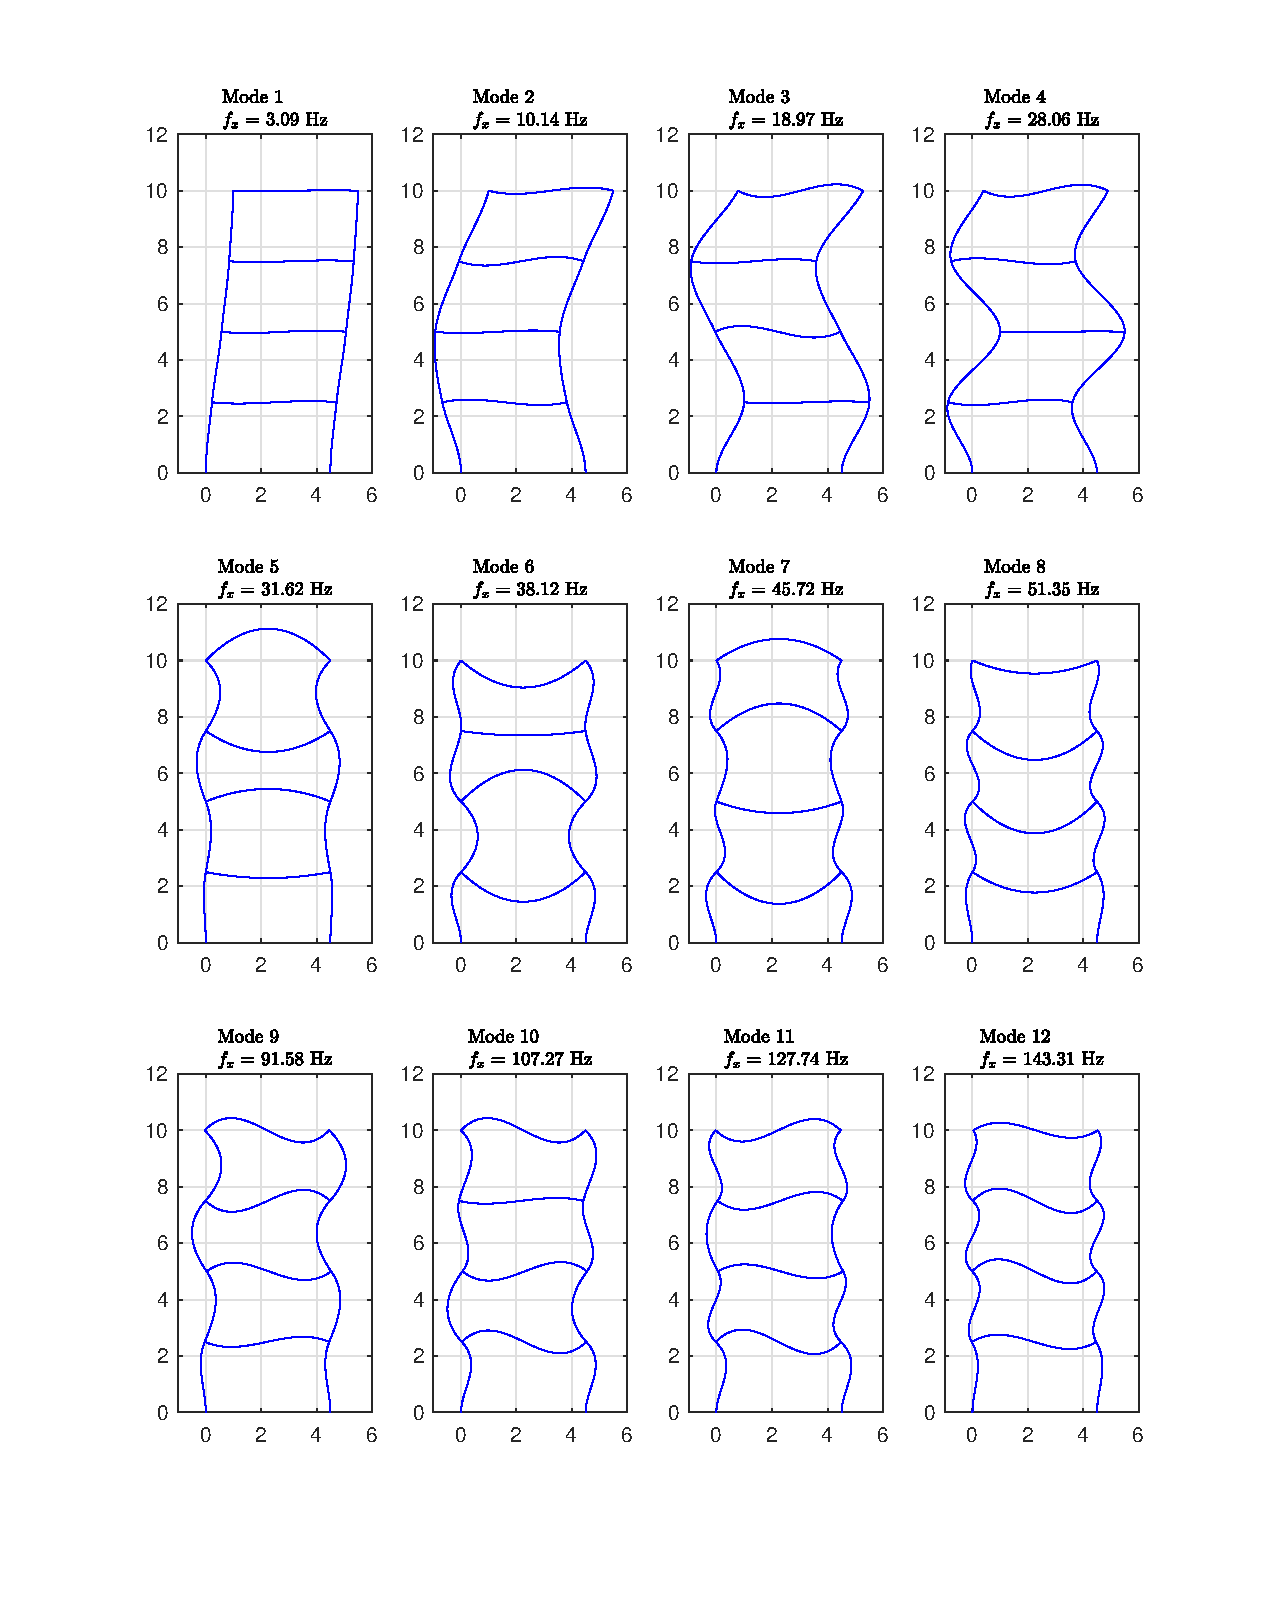
\includegraphics[width=16cm]{Mode_Shapes_X.eps}
\label{fig: I.1 - modes shapes x}
 \caption{Sketches of the 12 natural modes and their respective natural frequencies for the 2D frame in the global $(X,Z)$ axis.}
\end{figure}
\newpage
\begin{figure}
    \centering
    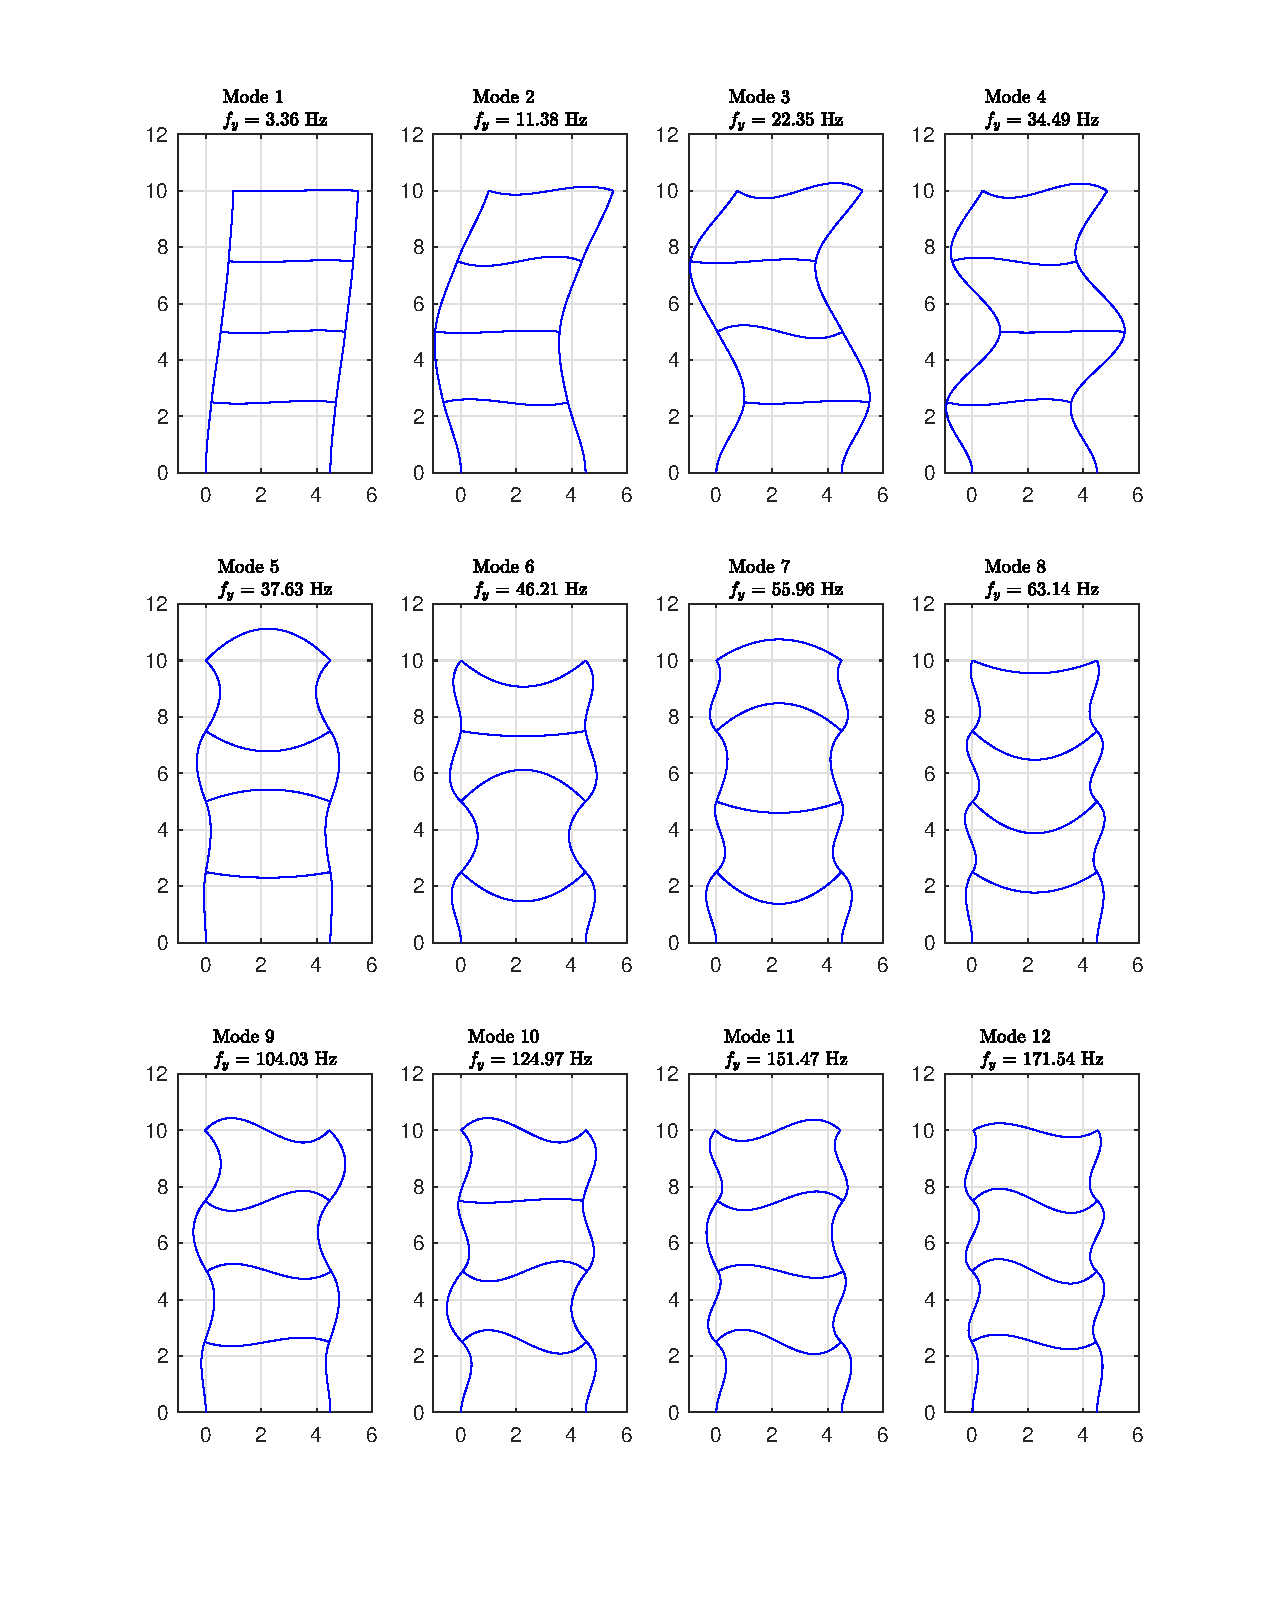
\includegraphics[width=16cm]{Mode_Shapes_Y.eps}
\label{fig: I.1 - modes shapes y}
 \caption{Sketches of the 12 natural modes and their respective natural frequencies for the 2D frame in the global $(Y,Z)$ axis.}
\end{figure}
\newpage
\subsection{Other Modal Parameters}
The other modal parameters for the low rise building include the modal mass, modal stiffness, modal participation factor, and the effective modal mass. The derivation of these parameters is outlined in the following sections.
\subsubsection{Modal Mass}
\paragraph{} The modal mass, $M_i$, of mode $(i = 1,2,...,12)$, is shown in \textsc{Equation}\,\ref{eq:I.1 - Modal Mass - Low Rise}
\begin{equation}
    M_i = \phi_i^T\,M_{X,Y}\,\phi_i
    \label{eq:I.1 - Modal Mass - Low Rise}
\end{equation}
\paragraph{}Where,
\begin{itemize}
\begin{small}
    \item $\phi_i$ is the shape vector of the mode, $(i = 1,2,...,12)$ $[-]$
    \item $M_{X,Y}$ is the mass matrix $[kg]$
\end{small}
\end{itemize}
\subsubsection{Modal Participation Factor}
\paragraph{} The modal participation factor, $MPF_i$, of each element, $(i = 1,2,...,12)$, of the structure is derived from \textsc{Equation}\,\eqref{eq:I.1 - Modal Participation Factor - Low Rise} below.
\begin{equation}
    {MPF}_i = \dfrac{\phi_i\,M\,r}{M_i}
    \label{eq:I.1 - Modal Participation Factor - Low Rise}
\end{equation}
\paragraph{}Where,
\begin{itemize}
\begin{small}
     \item $M$ is the mass matrix $[kg]$
    \item $\phi_i$ is the shape vector of mode, $(i = 1,2,...,12)$ $[-]$
    \item $M_i$ is the modal mass for a specific mode $(i = 1,2,...,12)$, as determined in \textsc{Equation}\,\eqref{eq:I.1 - Modal Mass - Low Rise} $[kg]$
     \item $r$ is a vector that is equal to zero for any DOF that are not parallel to the action of earthquake motion, and is equal to one for any DOF that are parallel to the earthquake motion $[-]$
\end{small}
\end{itemize}
\subsubsection{Effective Modal Mass}
\paragraph{} The effective modal mass, $M_{eff,i}$, of the mode,  $(i = 1,2,...,12)$, within the low rise structure is a produced using \eqref{eq:I.1 - Effective Modal Mass - Low Rise}. below.
\begin{equation}
    M_{eff,i} = {MPF}_i\,\phi_i^T\,M\,r
    \label{eq:I.1 - Effective Modal Mass - Low Rise}
\end{equation}
\paragraph{}Where,
\begin{itemize}
    \item $MPF_i$ is the modal participation factor for a specific mode, $(i = 1,2,...,12)$
    \item $\phi_i$ is the mode of a specific element, $(i = 1,2,...,12)$
    \item $M_{X,Y}$ is the mass matrix in the (X,Z), or (Y,Z) direction as specified in \textsc{Equation}\,\eqref{eq : I.1 - local mass}
    \item $r$ is a vector that is equal to zero for any DOF that are not parallel to the action of earthquake motion, and is equal to one for any DOF that are parallel to the earthquake motion $[-]$
\end{itemize}
 \begin{table}[h]
 \begin{small}
    \centering
    \begin{tabular}{c|c|c|c|c|c}
        Mode & $M_i$ $[kg]$ & $MPF_i$ $[-]$ & $M_{eff,i}$ $[kg]$ & $\dfrac{M_{eff,i}}{M_{tot}}$ $[-]$ & $\sum\dfrac{M_{eff,i}}{M_{tot}}$ $[-]$\\
        \hline
       $1$ & $27,153$ & $1.30$ & $45,501$ & $0.81$ & $0.81$ \\
       $2$ & $35,316$ & $0.42$ & $6,649$ & $0.11$ & $0.92$\\
       $3$ & $32,921$ & $0.27$ & $2,682$ & $0.04$ & $0.96$\\
       $4$ & $44,513$ & $0.13$ & $945$ & $0.01$ & $0.97$\\
        $5$ & $12,493$ & $1.09$x$10^{-15}$ & $1.17$x$10^{-27}$ & $2.62$x$10^{-31}$ & $0.97$\\
       $6$ & $21,543$ & $-1.09$x$10^{-16}$ & $1.34$x$10^{-27}$ & $1.52$x$10^{-32}$ & $0.97$\\
       $7$ & $19,345$ & $4.54$x$10^{-16}$ & $1.81$x$10^{-26}$ & $7.04$x$10^{-32}$ & $0.97$\\
       $8$ & $20,156$ & $-4.00$x$10^{-16}$ & $6.09$x$10^{-28}$ & $5.65$x$10^{-32}$ & $0.97$\\
        $9$ & $4,573$ & $0.06$ & $16.72$ & $0.00026$ & $0.97$\\
       $10$ & $3,536$ & $0.10$ & $51.08$ & $0.00067$ & $0.97$\\
       $11$ & $4,173$ & $-0.07$ & $25.94$ & $0.00035$ & $0.97$\\
       $12$ & $3,390$ & $0.04$ & $5.78$ & $0.00008$ & $0.97$\\
    \end{tabular}
    \caption{Modal Masses of each Mode of the Low Rise Building in (X,Z) direction}
    \label{tab:low rise - modal properties x}
    \end{small}
\end{table}
 \begin{table}[h]
 \begin{small}
    \centering
    \begin{tabular}{c|c|c|c|c|c}
        Mode & $M_i$ $[kg]$ & $MPF_i$ $[-]$ & $M_{eff,i}$ $[kg]$ & $\dfrac{M_{eff,i}}{M_{tot}}$ $[-]$ & $\sum\dfrac{M_{eff,i}}{M_{tot}}$ $[-]$\\
        \hline
        $1$ & $26,613$ & $1.31$ & $45,503$ & $0.79$ & $0.79$\\
       $2$ & $34,267$ & $0.44$ & $6,649$ & $0.12$ & $0.91$\\
       $3$ & $33,303$ & $0.28$ & $2,682$ & $0.05$ & $0.96$\\
       $4$ & $40,533$ & $0.15$ & $945$ & $0.02$ & $0.97$\\
        $5$ & $11,757$ & $3.16$x$10^{-16}$ & $1.17$x$10^{-27}$ & $5.48$x$10^{-35}$ & $0.97$\\
       $6$ & $20,191$ & $2.57$x$10^{-16}$ & $1.34$x$10^{-27}$ & $7.51$x$10^{-33}$ & $0.97$\\
       $7$ & $19,043$ & $-9.76$x$10^{-16}$ & $1.81$x$10^{-26}$ & $1.68$x$10^{-33}$ & $0.97$\\
       $8$ & $19,582$ & $-1.76$x$10^{-16}$ & $6.09$x$10^{-28}$ & $7.28$x$10^{-33}$ & $0.97$\\
        $9$ & $2,952$ & $-0.08$ & $16.72$ & $0.00033$ & $0.97$\\
       $10$ & $5,132$ & $-0.1$ & $51.08$ & $0.00089$ & $0.97$\\
       $11$ & $3,452$ & $0.09$ & $25.94$ & $0.00044$ & $0.97$\\
       $12$ & $3,250$ & $0.04$ & $5.78$ & $0.00009$ & $0.97$\\
    \end{tabular}
    \caption{Modal Masses of each Mode of the High Rise Building}
    \label{tab:low rise - modal properties y}
\end{small}
\end{table}
\paragraph{}From the tables above, it is clear that the modal mass shows similar results for mode shapes 1, 2, 3, and 4, mode shapes, 5, 6, 7, and 8, and mode shapes 9, 10, 11, and 12. Showing that the first four modes move a larger mass of the building than that of the latter. It can be seen in the last four modes that they move a whole magnitude less of the building, which is quite significant. Moving across the table and looking at the modal participation factor for each of the modes it can be seen that the first mode is the most significant, having it be the only mode with a participation factor greater than one. This results in an effective modal mass of the first mode that is a magnitude larger than the next largest effective modal mass. The modal participation factors produced for modes 5, 6, 7, and 8 are smaller than the results of the other modes. As previously explained, these four mode shapes are influenced by the same moments. Therefore, it has been hypothesized that these extremely low values for the participation factor of these modes is a result of the geometry of the structure. 
\paragraph{}Additionally, the modal factors have been presented in the table. These values are used to quantify, by mass, the per-mode contribution throughout an entire building followed by taking the sum of this result to determine the percent, by mass, of which each mode is responsible for. This factor is important because to create an accurate response in the later sections of this report, the sum of these values must be greater than 0.9, so that more than $90\%$ of the mass of the building is accounted for. The results show that the 12 modes account for $97\%$ of the mass of the low rise building in both directions. Therefore the responses of the structure as subsequently produced in the following chapters of this report can be considered accurate.  
\subsubsection{Modal Stiffness}
\paragraph{} The modal stiffness, $K_i$, the stiffness of the structure at the specified mode, $(i = 1,2,...,12)$, given in \textsc{Equation}\,\eqref{eq:I.1 - Modal Stiffness - High Rise} below.
\begin{equation}
    K_i = M_i\,\omega_i^2
    \label{eq:I.1 - Modal Stiffness - Low Rise}
\end{equation}
\paragraph{}Where,
\begin{itemize}
\begin{small}
    \item $M_i$ is the modal mass determined in \textsc{Equation}\,\eqref{eq:I.1 - Modal Mass - Low Rise} $[kg]$
    \item $\omega_i$ is the frequency of mode, $(i = 1,2,..,12)$ given in \textsc{Equation}\,\eqref{eq: I.1 - eig continu} $[rad/s]$
\end{small}
\end{itemize}
\begin{table}[h]
    \centering
    \begin{tabular}{c|c|c}
        Mode & Stiffness in (X,Z) plane $[MN]$ & Stiffness in (Y,Z) plane $[MN]$\\
        \hline
         $1$ & $10$ & $12$\\
         $2$ & $124$ & $154$\\
         $3$ & $467$ & $658$\\
         $4$ & $1,083$ & $1,655$\\
         $5$ & $493$ & $677$\\
         $6$ & $1,236$ & $1,782$\\
         $7$ & $1,597$ & $2,381$\\
         $8$ & $2,098$ & $3,157$\\
         $9$ & $1,220$ & $1,355$\\
         $10$ & $1,606$ & $2,310$\\
         $11$ & $2,280$ & $3,162$\\
         $12$ & $2,749$ & $3,938$\\
    \end{tabular}
    \caption{Modal Masses of each Mode of the High Rise Building}
    \label{tab:low rise modal stiffness}
\end{table}
\paragraph{}\textsc{Table}\,\ref{tab:low rise modal stiffness} shows the numerical results of the modal stiffness of the low rise building in both the (X,Z) and (Y,Z) plane. The results presented in $[MN]$ increase proportionally with mode number.
\section{High Rise Building}
\begin{figure}
    \centering
    \includegraphics[width=6cm]{High_rise_structure.jpeg}
    \caption{High Rise Structure}
    \label{fig:I.2 - high rise structure}
\end{figure}
\paragraph{}The high rise building is analyzed as a continuous cantilever column. The top of the building acts as a free end (the moment and force at this point are both equal to zero) and the base of the building acts as a clamped end (the displacement and velocity are both be equal to zero) as shown in \textsc{Figure}\,\ref{fig:I.2 - high rise structure}. It is assumed that, the mass per unit length, Young's Modulus for concrete, and inertia for the building will remain constant along the length of the cantilever column. \textsc{Figure}\,\ref{fig:I.1 High Rise Building Aerial} below is representative of the aerial view looking into the Z-plane of the high rise building being studied. This image shows that the building is composed of a reinforced concrete (RC) central core surrounded by four glass panels. The RC core is the structural component of the building, therefore its dimensions will be used to determine the moment of inertia of the structure. The assumptions that have been made for the analysis of this building include that, like that of the low rise building, the three-dimensional structure will be analyzed as two separate two-dimensional structures. The building will be analyzed as a continuous system, in which the mass per unit length, moment of inertia, and Young's Modulus for concrete will be uniform throughout the structure. It will be treated like a cantilever beam with a distributed mass and elasticity. 
\begin{figure} [h]
    \centering
    \includegraphics[width=14cm]{High_Rise_z.jpeg}
    \caption{High Rise Building Looking Down Z-axis}
    \label{fig:I.1  High Rise Building Aerial}
\end{figure}
\subsection{Mass} 
\paragraph{}To determine the mass per unit length, $\bar{m}$ $[kg/m]$, of the high rise building the total mass of the structure must first be determined. Please note that the dead load used in the calculation takes the weight of the slab into account, which is why the weight of the slab is not included in the calculation. Additionally, both the dead load and live loads are not applied to the concrete core. This is because there will not be any human activity in this area as the core is purely structural acting as four walls, whose self weights have already been calculated. 

\begin{equation}
    m = 2\,\rho_c\,t_c\,(D_c-2t_c)\,+\,2\,\rho_c\,(t_c\,W_c)\,+\,(G+\phi\,Q)(W\,+\,D)\,+\,2\,\rho_{gl}\,t_{gl}\,D+\,2\,\rho_{gl}\,t_{gl}\,W
    \label{eq:I.1 - High Rise Total Mass}
\end{equation}
\begin{equation}
    \bar{m} = \dfrac{m}{L}
    \label{eq:I.1 - High Rise Mass Per Unit}
\end{equation}
\paragraph{}Where,
\begin{itemize}
\begin{small}
    \item $m$ is the total mass of the high rise building $[kg]$
    \item $\bar{m}$ is the mass per unit length of the high rise building $[kg/m]$
    \item $\rho_c$ is the density of concrete given in \textsc{Table}\,\ref{tab: specifications - material properties} $[kg/m^3]$
    \item $t_c$ is the thickness of the reinforced concrete core given in \textsc{Table}\,\ref{tab: Specifications - Design HighRB} $[m]$
    \item $D_c$ is the depth of the reinforced concrete core, parallel to the Y-axis, given in \textsc{Table}\,\ref{tab: Specifications - Design HighRB} $[m]$
    \item $W_c$ is the width of the reinforced concrete core, parallel to the X-axis, given in \textsc{Table}\,\ref{tab: Specifications - Design HighRB} $[m]$
    \item $G$ is the dead load in the high rise building given in \textsc{Table}\,\ref{tab: Specifications - Design HighRB} $[kg/m^2]$
    \item $Q$ is the live load in the high rise building given in \textsc{Table}\,\ref{tab: Specifications - Design HighRB} $[kg/m^2]$
    \item $W$ is the width of the high rise building, parallel to the X-axis, given in \textsc{Table}\,\ref{tab: Specifications - Design HighRB} $[m]$
    \item $D$ is the depth of the high rise building, parallel to the Y-axis, given in \textsc{Table}\,\ref{tab: Specifications - Design HighRB} $[m]$
    \item $\rho_{gl}$ is the density of the glass given in \textsc{Table}\,\ref{tab: specifications - material properties} $[kg/m^3]$
    \item $t_{gl}$ is the thickness of the glass given in \textsc{Table}\,\ref{tab: Specifications - Design HighRB} $[m]$
       \item $L$ is the height of the high rise building given in \textsc{Table}\,\ref{tab: Specifications - Design HighRB} $[m]$
\end{small}
\end{itemize}
\paragraph{}Using \textsc{Equation}\,\eqref{eq:I.1 - High Rise Total Mass} the total mass of the high rise building was determined to be $8,2785\,kg$. The mass per unit length of the building, determined using \textsc{Equation}\,\eqref{eq:I.1 - High Rise Mass Per Unit}, is $811.62\,kg/m$.

\subsection{Inertia} 
\paragraph{}The moment of inertia, $I$ $[m^4]$, in the high rise building is derived from the dimensions of the reinforced concrete core in as shown in \textsc{Equation}\,\eqref{eq:I.1 - High Rise Inertia} below. Only the RC core dimensions are used because the core is the only structural part of the building. Refer to \textsc{Figure}\,\ref{fig:I.1  High Rise Building Aerial} for a visual representation of these dimensions.
\begin{equation}
    I = 2\,\left(\dfrac{(D_c-2t_c)^3\,t_c}{12}\right)+2\,\left(\left(\dfrac{t_c^3\,W_c}{12}\right)+\left(\dfrac{D_c-t_c}{2}\right)^2\,W_c\,t_c\right)
    \label{eq:I.1 - High Rise Inertia}
\end{equation}
\paragraph{}Where,
\begin{itemize}
\begin{small}
    \item $D_c$ is the depth of the reinforced concrete core given in \textsc{Table}\,\ref{tab: Specifications - Design HighRB} $[m]$
     \item $t_c$ is the thickness of the reinforced concrete core given in \textsc{Table}\,\ref{tab: Specifications - Design HighRB} $[m]$
     \item $W_c$ is the width of the reinforced concrete core given in \textsc{Table}\,\ref{tab: Specifications - Design HighRB} $[m]$
\end{small}
\end{itemize}
\paragraph{}The values for the inertia of the high rise building in the (X,Z) and (Y,Z) planes are as follows, $I_x = 337.64m^4$, and $I_y = 536.58m^4$. The width of the high rise building is significantly larger along the $X$ direction making it more difficult for the building to bend in that direction resulting in a smaller moment of inertia in the (X,Z) plane than that of the (Y,Z) plane.
\subsection{Eigenmodes and Eigenfrequencies}
\paragraph{} The natural frequencies and natural modes of the structure are determined by solving the the equation governed by the spacial variable in the decoupled equation of the free vibration system shown in \textsc{Equation}\,\eqref{eq: I.1 - eig continu}. The solution of this equation using the boundary conditions is the eigenmode function and given in \textsc{Equation}\,\eqref{eq: I.1 - function of the eigenmodes}. In this case we are going to study the first four mode shapes $m=1,2,3,4$, for which, 
\begin{equation}
    \beta_1\,H=1.8751,\,\,\,\beta_2\,H=4.6941,\,\,\,\beta_3\,H=7.8548,\,\,\,\beta_4\,H=10.996
    \label{eq:I.1: betas}
\end{equation}
\paragraph{}With, $H$ $[m]$ being the total height of the high rise building.
\paragraph{} In this equation the second and fourth coefficients are equal to zero, corresponding to the boundary conditions previously stated.
\begin{equation}
\left\lbrace
\begin{array}{l}
     \dfrac{d^2q(t)}{dt^2}+\omega^2\,q(t) = 0 \\ \\
     \dfrac{d^2(E_c\,I\,\frac{d\phi(x')}{dx}}{dx^2}-\omega^2\,\bar{m}\,\phi(x)=0
\end{array}
\right.
\label{eq: I.1 - eig continu}
\end{equation}
\paragraph{}Where,
\begin{itemize}
\begin{small}
    \item $q$ is the modal coordinate vector $[m]$
    \item $\phi$ is the modal shape matrix $[-]$
    \item $E_c$ is the Young's Modulus for Concrete given in \textsc{Table}\,\ref{tab: specifications - material properties} $[N/m^2]$
    \item $I$ is the moment of interia determined in \textsc{Equation}\,\eqref{eq:I.1 - High Rise Inertia} $[m^4]$
    \item $\omega$ is the natural angular frequency vector $[rad/s]$
    \item $\bar{m}$ is the mass per unit length of the high rise building determined in \textsc{Equation}\,\eqref{eq:I.1 - High Rise Mass Per Unit} $[kg/m]$
    \item $x$ is the local coordinate along the height of the high rise $[m]$
\end{small}
\end{itemize}

\begin{equation}
     \phi_m(x)=C_1\,\left[(cos\beta_n\,x-cos\beta_n\,x-\dfrac{cosh\beta_n\,L+cos\beta_n\,L}{sinh\beta_n\,L+sin\beta_n\,L} (sinh\beta_n\,x-sin\beta_n\,x)\right]
 \label{eq: I.1 - function of the eigenmodes}
\end{equation}
\paragraph{}Where,
\begin{itemize}
\begin{small}
   \item $\phi_m$ is the shape of the mode $(m=1,2,3,4)$ $[-]$
   \item $C_1$ is an shape constant used to normalize the mode shapes$[-]$
   \item $x$ is the local coordinate along the height of the high rise $[m]$
   \item $\beta_n$ is the constant dependent on the mode being studied $n=1,2,3,4$ as determined in \textsc{Equation}\,\eqref{eq:I.1: betas} $[m^{-1}]$
   \item $L$ is the height of the high rise building given in \textsc{Table}\,\ref{tab: Specifications - Design HighRB} $[m]$
  \end{small}
\end{itemize}
\paragraph{}Please note that since the variables appearing in $\phi_m(x)$ are not dependent on the studied direction, so will be the same for both the (X,Z) and (Y,Z) planes. Once the mode shape matrix has been calculated it is normalized by $C_1$ to give the mode shape so that the greatest unit displacement of any mode shape is equal to 1.
\paragraph{}The eigenfrequencies in the (X.Z) plane are given by \textsc{Equation}\,\eqref{eq: I.1 - high rise - function of the eigenfrequencies x}.
\paragraph{}
\begin{equation}
\omega_{x,i} =
    \left\lbrace
    \begin{array}{c}
         \dfrac{3.516}{H^2}\,\sqrt{\dfrac{E_c\,I_y}{\bar{m}}}  \\
         \\
         \dfrac{22.03}{H^2}\,\sqrt{\dfrac{E_c\,I_y}{\bar{m}}}  \\
         \\
         \dfrac{61.70}{H^2}\,\sqrt{\dfrac{E_c\,I_y}{\bar{m}}} \\
         \\
         \dfrac{120.9}{H^2}\,\sqrt{\dfrac{E_c\,I_y}{\bar{m}}} \\
         \\
    \end{array}
    \right.
    \label{eq: I.1 - high rise - function of the eigenfrequencies x}
\end{equation}
\paragraph{}Where,
\begin{itemize}
\begin{small}
    \item $\omega_{x,i}$ is the natural angular frequency of specified mode in the (X,Z) plane, $(i = 1,2,3,4)$ $[rad/s]$
    \item $H$ is the height of the high rise building given in \textsc{Table}\,\ref{tab: Specifications - Design HighRB} $[m]$
    \item $E_c$ is the Young's Modulus for Concrete given in \textsc{Table}\,\ref{tab: specifications - material properties}$[N/m^2]$
    \item $I_y$ is the moment of inertia in the $Y$ direction, determined in \textsc{Equation}\,\eqref{eq:I.1 - High Rise Inertia} $[m^4]$
    \item $\bar{m}$ is the mass per unit length of the high rise building determined in \textsc{Equation}\,\eqref{eq:I.1 - High Rise Mass Per Unit} $[kg/m]$
\end{small}
\end{itemize}
\paragraph{}The same equation is used to determine the eigenfrequency values in the (Y,Z) plane, but uses $I_x$ rather than $I_y$.
\paragraph{}The natural frequency and natural period of the structure is determined using \textsc{Equation}\,\ref{eq:I.1 - HR - natural frequency} and \textsc{Equation}\,\ref{eq:I.1 - HR - natural period}. The results will be different for the (X,Z) and (Y,Z) planes, as it is dependent on the natural angular frequency which is directional dependent. The natural period represents the time it takes for the building to complete the cycle of vibrating from its original state to its largest modal displacement in one direction and then to that same modal displacement in the opposite direction and back to its original state. 
\begin{equation}
    f=\dfrac{\omega}{2\,\pi}
    \label{eq:I.1 - HR - natural frequency}
\end{equation}
\begin{equation}
    T=\dfrac{1}{f}
    \label{eq:I.1 - HR - natural period}
\end{equation}
\paragraph{}Where,
\begin{itemize}
\begin{small}
    \item $\omega$ is the natural angular frequency of the structure $[rad/s]$
    \item $f$ is the natural frequency of the structure $[Hz]$
    \item $T$ is the natural period of the structure $[s]$
\end{small}
\end{itemize}
\begin{figure}
    \centering
    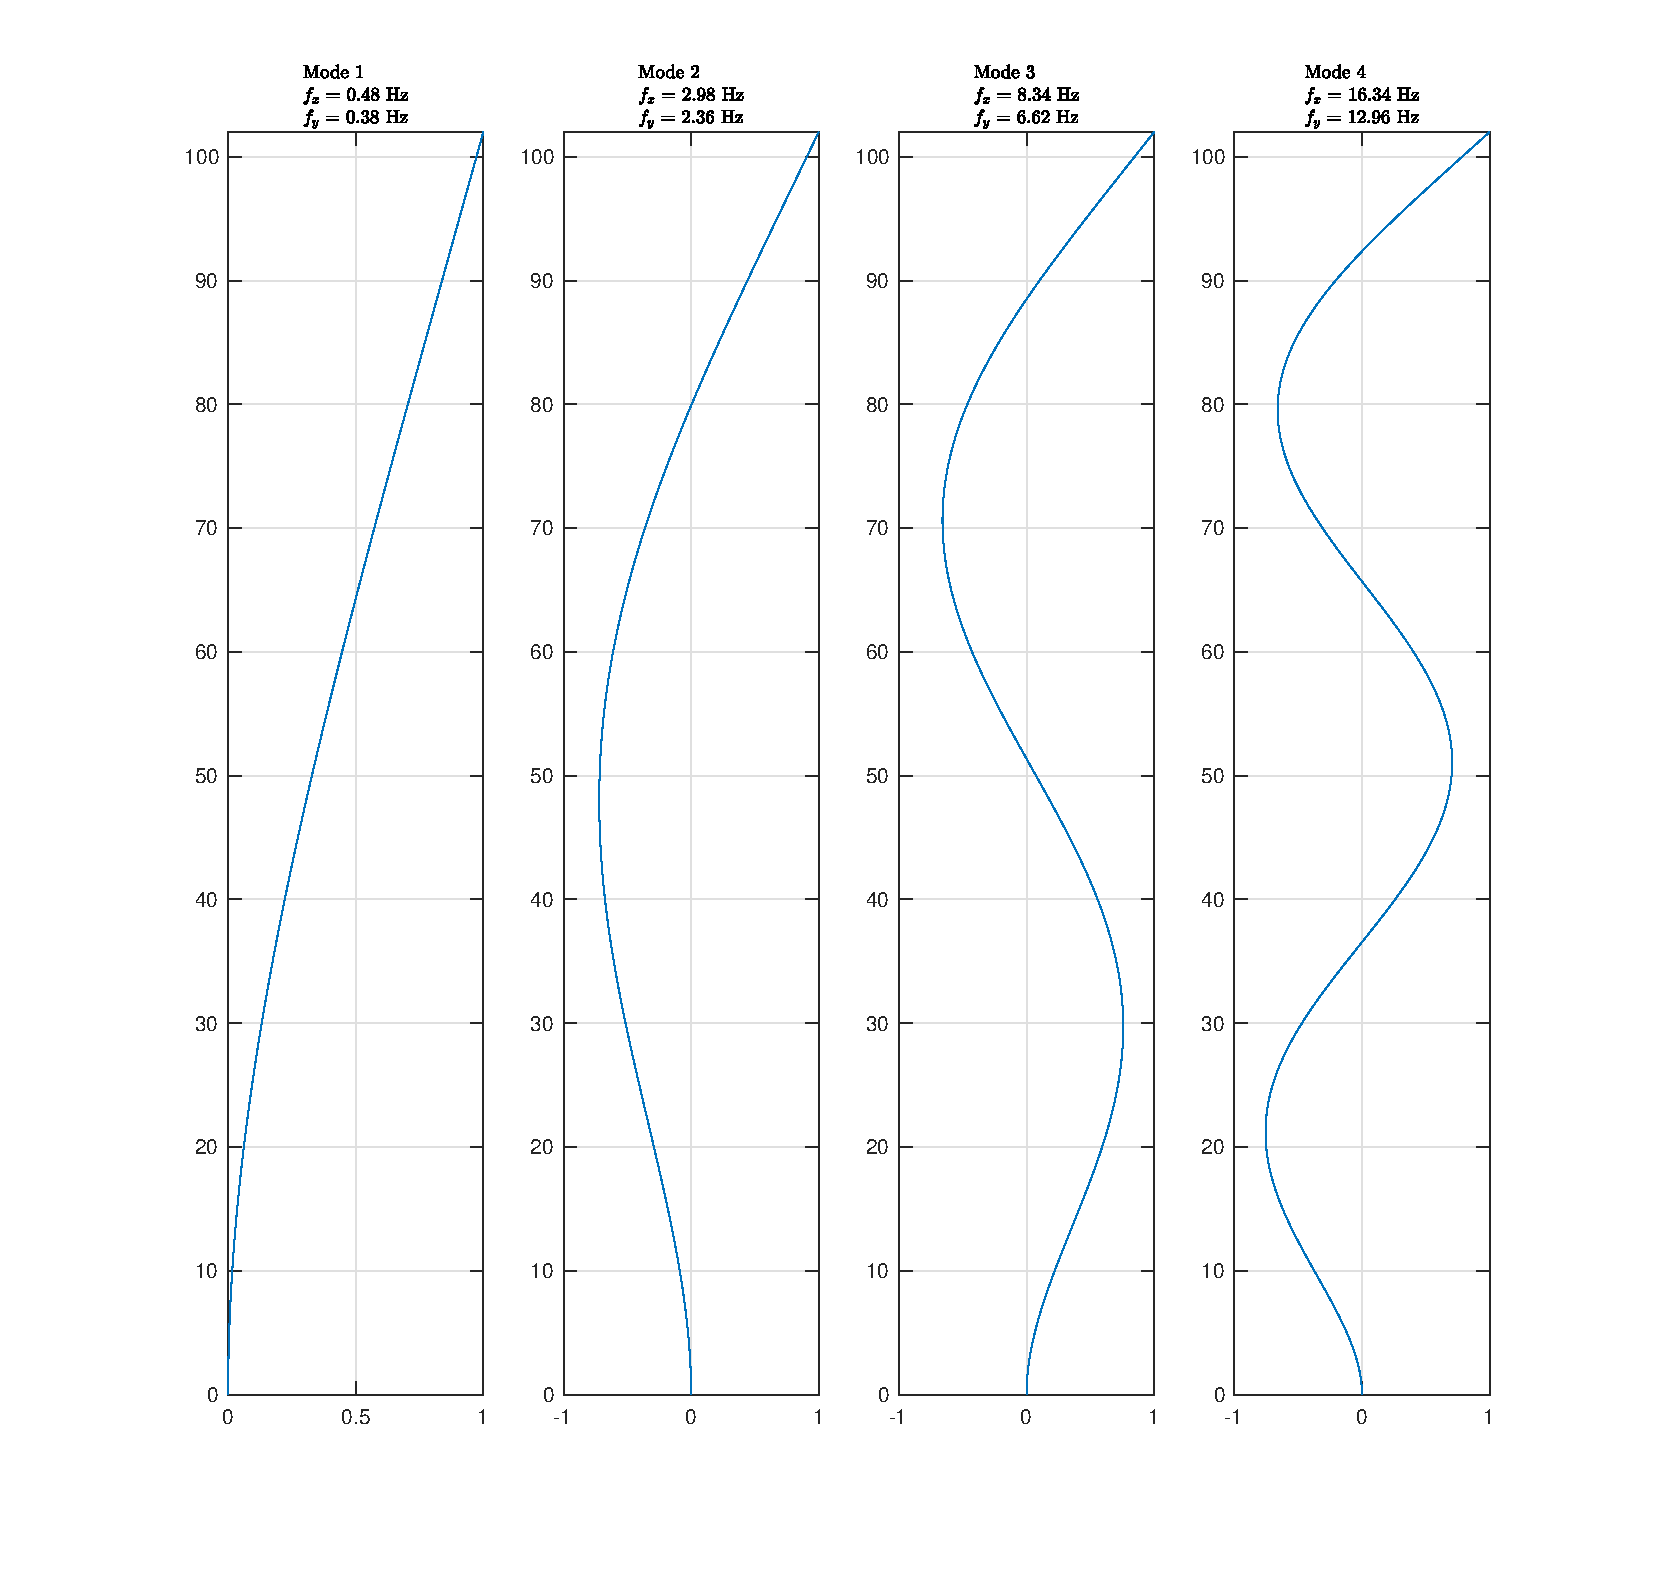
\includegraphics[width=16cm]{High_Rise_Modes.eps}
    \caption{Mode Shapes for the High Rise Building}
    \label{fig:I.2: High Rise Modes}
\end{figure}
\paragraph{}The mode shapes of the high rise building can be seen above in \textsc{Figure}\,\ref{fig:I.2: High Rise Modes}. The mode shapes produced are reflective of the mode shapes of a typical cantilever beam as expected. The first bending mode is a simple transverse deformation of the beam. With increasing mode numbers, the shapes of the modes become more complex, showing an increased amount of points with horizontal displacement. It should be noted that the displacement in the modes has been normalized, so that the maximum displacement in any of the mode shapes is equal to 1. It can be seen that the natural frequency of all modes is greater in the (X,Z) plane that that of the (Y,Z) plane. This is a direct result of the moment of inertia in the two planes. As shown in \textsc{Equation}\,\ref{eq: I.1 - high rise - function of the eigenfrequencies x}, the natural frequency in the (X,Z) plane is dependent on the moment of inertia in the Y direction. For this reason, the natural frequency of the structure is greater in the (X,Z) plane than the (Y,Z) plane.

\subsection{Other Modal Parameters}
\paragraph{}The other modal parameters of the high rise building include the modal mass, modal stiffness, modal participation factor, and effective modal mass. These parameters are necessary for the structural response as it allows the MDOF structure to be analyzed as a SDOF to simplify the derivation. The process in which these parameters are determined is outlined in the following sections.
\subsubsection{Modal Mass}
\paragraph{}The modal mass, $M_i$, of the continuous system is determined using\textsc{Equation}\,\eqref{eq:I.1 - Modal Mass - High Rise} below. The modal mass is a numerical representation of the mass of the mode.
\begin{equation}
    M_i = \int_{0}^{H}\,\bar{m}\,\phi_i^2(x)dx
    \label{eq:I.1 - Modal Mass - High Rise}
\end{equation}
\paragraph{}Where,
\begin{itemize}
\begin{small}
    \item $H$ is the height of the high rise building given in \textsc{Table}\,\ref{tab: Specifications - Design HighRB}
    \item $\bar{m}$ is the mass per unit length of the high rise building determined in \textsc{Equation}\,\eqref{eq:I.1 - High Rise Mass Per Unit}
    \item $\phi_i$ is the specific mode $(i = 1,2,3,4)$
    \item $x$ is the local coordinate along the height of the high rise $[m]$
\end{small}
\end{itemize}
\paragraph{}Note: for integrals we will use trapezoidal integration.
\subsubsection{Modal Participation Factor}
\paragraph{}The modal participation factor, $MPF_i$, for a specific mode, $(i = 1,2,3,4)$, of the high rise building has been determined using \textsc{Equation}\,\eqref{eq:I.1 - Modal Participation Factor - High Rise} below.
\begin{equation}
    MPF_i = \dfrac{\int_{0}^{H}\,\bar{m}\,\phi_i(x)dx}{M_i}
    \label{eq:I.1 - Modal Participation Factor - High Rise}
\end{equation}
\paragraph{}Where,
\begin{itemize}
\begin{small}
    \item $H$ is the height of the high rise building given in \textsc{Table}\,\ref{tab: Specifications - Design HighRB} $[m]$
    \item $\bar{m}$ is the mass per unit length  given in \textsc{Equation}\,\eqref{eq:I.1 - High Rise Mass Per Unit} $[kg/m]$
    \item $\phi_i$ is the specific mode $(i = 1,2,3,4)$ given in $[-]$ \textsc{Equation}\,\eqref{eq: I.1 - function of the eigenmodes}
     \item $x$ is the local coordinate along the height of the high rise $[m]$
    \item $M_i$ is the modal mass for a specific mode $(i = 1,2,3,4)$, as determined in \textsc{Equation}\,\eqref{eq:I.1 - Modal Mass - High Rise} $[kg]$
\end{small}
\end{itemize}
\subsubsection{Effective Modal Mass}
\paragraph{}The effective modal mass, $M_{eff,i}$, for a specific mode, $(i = 1,2,3,4)$, have been determined using \textsc{Equation}\,\eqref{eq:I.1 - Effective Modal Mass - High Rise} below. 
\begin{equation}
    M_{eff,i}= MPF_i\,\int_{0}^{H}\,\bar{m}\,\phi_i(x)dx
    \label{eq:I.1 - Effective Modal Mass - High Rise}
\end{equation}
\paragraph{}Where,
\begin{itemize}
\begin{small}
    \item $MPF_i$ is the modal participation factor for a specific mode, $(i = 1,2,3,4)$
    \item $H$ is the height of the high rise building given in \textsc{Table}\,\ref{tab: Specifications - Design HighRB} $[m]$
    \item $\bar{m}$ is the mass per unit length given in \textsc{Equation}\,\eqref{eq:I.1 - High Rise Mass Per Unit} $[m/kg]$
    \item $\phi_i$ is the mode shape $(i = 1,2,3,4)$ given in \textsc{Equation}\,\eqref{eq: I.1 - function of the eigenmodes} $[-]$
    \item $x$ is the local coordinate along the height of the high rise $[m]$
\end{small}
\end{itemize}
\paragraph{}It is important to note that the parameters influencing the modal mass, $M_i$, are independent of the direction in which the structure is being studied. So the modal mass and the parameters dependent on it which include the modal participation factor and effective modal mass, are the same for both the (X,Z) and (Y,Z) planes. Conversely, the modal stiffness will be different for the (X,Z) and (Y,Z) planes as this parameter is also dependent on the natural angular frequencies of the modes, a variable that is dependent on the studied direction of the structure
\paragraph{}The resulting effective modal masses for the high rise building are shown below in \textsc{Table}\,\ref{tab:high rise effective modal mass}.
\begin{table}[h]
    \centering
    \begin{tabular}{c|c|c|c|c|c}
        Mode & $M_i$ $[kg]$ & $MPF_i$ $[-]$ & $M_{eff,i}$ $[kg]$ & $\dfrac{M_{eff,i}}{M_{tot}}$ $[-]$ & $\sum\dfrac{M_{eff,i}}{M_{tot}}$ $[-]$\\
        \hline
       $1$ & $8,267$ & $1.0007$ & $8,279$ & $0.61$ & $0.61$\\
       $2$ & $8,239$ & $-1.0023$ & $8,279$ & $0.19$ & $0.80$\\
       $3$ & $8,215$ & $1.0038$ & $8,278$ & $0.06$ & $0.87$\\
       $4$ & $8,190$ & $-1.0054$ & $8,278$ & $0.03$ & $0.90$\\
    \end{tabular}
    \caption{Modal Masses of each Mode of the High Rise Building}
    \label{tab:modal properties}
\end{table}
\paragraph{}The numerical results of the modal mass, modal participation factor, and effective modal mass have been summarized in \textsc{Table}\,\ref{tab:modal properties}. Analyzing the numerical values produced, it is evident that the effective modal masses have less variability for each of the modes than that of the modal mass. This is due to the fact that the modal masses are inversely proportional to the mode number, while the modal participation factor is proportional to the mode number. 
\paragraph{}The last two values in the \textsc{Table}\,\ref{tab:modal properties} are the participating masses of the modes. It is used as reference values to determine if the number of modes will produce an accurate response of the building, and can be seen as a percentage of the building's mass activated by the mode.. This is done buy summing the results of the effective modal mass as a fraction of the total mass of the structure. The sum of these fractions needs to be equal to $0.9$ to deem the response of the building accurate. This is because the effective modal mass needs to account for at a minimum $90\%$ of the total mass of the structure. \textsc{Table}\,\ref{tab:modal properties} shows that with a mode number of four, the analysis will only reflect the response of $40\%$ of the mass of the high rise building. This should be noted, and will be further discussed in later sections of this report as these modal parameters will be used to determine the structural response of the building.
\subsubsection{Modal Stiffness}
\paragraph{} The modal stiffness, $K_i$, the stiffness of the structure at the specified mode, $(i = 1,2,3,4)$, given in the overarching equation, \textsc{Equation}\,\eqref{eq:I.1 - Modal Stiffness - High Rise} below. This equation was used to verify the values produced from \textsc{Equation}\,\eqref{eq:I.1 - Modal Stiffness - High Rise - complicated}
\begin{equation}
    K_i  = M_i\,\omega_i^2
    \label{eq:I.1 - Modal Stiffness - High Rise}
\end{equation}
\begin{equation}
    K_i=\int^H_0\,\phi_m(x)\,\left(E_c\,I\,\phi^"_m(x)\right)^"\,dx
    \label{eq:I.1 - Modal Stiffness - High Rise - complicated}
\end{equation}
\paragraph{}Where,
\begin{itemize}
\begin{small}
   \item $M_i$ is the modal mass for a specific mode $(i = 1,2,3,4)$, as determined in \textsc{Equation}\,\eqref{eq:I.1 - Modal Mass - High Rise} $[kg]$
    \item $\omega_i$ is the natural angular frequency of specified mode, $(i = 1,2,3,4)$ given in \textsc{Equation}\,\eqref{eq: I.1 - high rise - function of the eigenfrequencies x} $[rad/s]$
    \item $H$ is the height of the high rise building given in \textsc{Table}\,\ref{tab: Specifications - Design HighRB} $[m]$
    \item $\phi_m(x)$ is the displacement of mode shape $(m=1,2,3,4)$ $[m]$
    \item $E_c$ is the Young's Modulus for concrete given in \textsc{Table}\,\ref{tab: specifications - material properties} $kg/m^3$
    \item $I$ is the moment of inertia in either the (X,Z) or (Y,Z) direction, given in \textsc{Equation}\,\eqref{eq:I.1 - High Rise Inertia}
    \item $\phi^{""}_m(x)$ is calculated analytically by the fourth derivation of \textsc{Equation}\,\eqref{eq : I.1 - local horizontal displacement in each mode}
\end{small}
\end{itemize}
\paragraph{}Using this equation the modal stiffnesses were calculated. As previously discussed at the beginning of this section, the stiffness of each mode is not the same for the (X,Z), and (Y,Z) planes as the natural angular frequency is dependent on the structures studied direction. The modal stiffness for both studied directions has been presented below in \textsc{Table}\,\ref{tab:high rise modal stiffness}
\begin{table}[h]
    \centering
    \begin{tabular}{c|c|c}
        Mode & Stiffness in (X,Z) plane $[kN]$ & Stiffness in (Y,Z) plane $[kN]$\\
        \hline
         1 & 510 & 478\\
         2 & 320 & 299\\
         3 & 895 & 839\\
         4 & 175 & 164\\
    \end{tabular}
    \caption{Modal Masses of each Mode of the High Rise Building}
    \label{tab:high rise modal stiffness}
\end{table}
\paragraph{}Here it can be seen that the stiffness increases with the mode number in both the (X,Z) and (Y,Z) directions, as expected. This is because as the mode number increases, so does its respective natural angular frequency. The natural angular frequency is proportional to the stiffness of the mode, and in turn the mode number. The stiffness of the modes is consistently larger in the (X,Z) plane than in the (Y,Z) plane. This is correct, and is representative of the fact that the width of the building is larger in the (X,Z) plane than in the (Y,Z) plane. The ease of bending moment in an element is inversely proportional to the stiffness of the element. In the case of the structure under study it is easier to bend in the (Y,Z) plane than the (X,Z) plane which is consistent with the results.


\chapter{Structural Response - Modal Response Analysis}
This section outlines the steps to determine the total seismic response of both the low rise and high rise buildings using the modal response spectrum analysis method. In that aim, the Eurocode 8 elastic spectrum type 1 and the Eurocode 8 design spectrum will be used to determine the modal and total displacements, and the modal and total section forces. These section forces including both the bending moment and shear forces. 

\section{Low Rise Building}
The modal response of the low rise building has been analyzed in both the (X,Z) and (Y,Z) directions. The elastic and inelastic response of the structure is analyzed with the horizontal elastic response spectrum and the horizontal design response spectrum, respectively. The horizontal spectrum is being used because it has been hypothesized that the earthquake generates only horizontal accelerations. For the structure, the elastic spectrum will be used to determine the modal elastic displacements and the total elastic displacements. The design spectrum will be used to determine the modal design displacements, the total design displacements, as well as the modal section forces, and total section forces. 
\subsection{Acceleration Spectrum}\label{sec: Elastic Modal Displacmenets}
\paragraph{} The elastic modal and total responses of the building are dependent on the elastic response, therefore the first step in this process is to determine it. The elastic analysis is based on the horizontal elastic acceleration spectrum corresponding to the Type 1 seismic event. As given in the Eurocode, a Type 1 seismic event corresponds to a surface wave magnitude $M_s\,>\,5.5$. The analytic formation of this elastic acceleration spectrum is given in \textsc{Equation}\,\eqref{eq:I.2 - Low Rise - Elastic Spectrum} 
\paragraph{}The modal displacements of the low rise building are determined using the horizontal elastic response spectrum. This analysis uses the specifications determined by Eurocode 8 elastic spectrum Type 1, surface wave maginitude, $M_s\,>\,5.5$. These specifications outline the values for $S$, $T_B$, $T_C$, and $T_D$ which correspond to the soil type, D, on which the structure will be built. These values can be found in \textsc{Table} \ref{tab: specifications - seismic}. These specifications are part of the Nationally Determined Parameters (NDP) within Eurocode 8, but for the analysis the suggested Eurocode specifications have been used. The horizontal elastic response spectrum must be determined first, and then can be used to determine the modal displacements of the structure.
\paragraph{}Before outlining the steps of the elastic spectrum, the derivation of the design ground acceleration should be detailed, shown in \textsc{Equation}\,\eqref{eq:I.2 - design ground acceleration}. It should be noted that the design ground acceleration produced with this will be for soil type A. For this analysis soil type D is used, this is accounted for in the next step with the use of the soil type D's corresponding soil factor, $S$.
\begin{equation}
    a_g = a_{gR}\,\lambda_1
    \label{eq:I.2 - design ground acceleration}
\end{equation}
\paragraph{}Where,
\begin{itemize}
\begin{small}
    \item $a_g$ is the design ground acceleration for soil type A $[g]$
    \item $a_{gR}$ is the reference peak ground acceleration, an NDP parameter within Eurocode 8 for a return period of 475 years, given in \textsc{Table}\,\ref{tab: specifications - seismic} $[g]$
    \item $\lambda_1$ is the importance factor of the corresponding importance class of the structure, given in \textsc{Table}\,\ref{tab: specifications - seismic} $[-]$
\end{small}
\end{itemize}
\paragraph{} The elastic spectrum, $S_{e,a}(T)$, is derived from \textsc{Equation} \eqref{eq:I.2 - Low Rise - Elastic Spectrum} which determines the spectral acceleration in terms of gravity for a given period \cite{EC8}. 
\begin{equation}
S_{e,a}\,(T) = 
\left\lbrace
\begin{array}{cl}
     a_g\,S\,\left[1\,+\,\dfrac{T}{T_B}\,(2.5\eta\,-\,1)\right] & \mathrm{for}\,\,\,0s\,\geq\,T\,\geq\,T_B  \\ \\
     a_g\,S\,2.5\eta & \mathrm{for}\,\,\,T_B\,\geq\,T\,\geq\,T_C \\ \\
     a_g\,S\,2.5\eta\left[\dfrac{T_C}{T}\right] & \mathrm{for}\,\,\, T_C\,\geq\,T\,\geq\,T_D \\ \\
     a_g\,S\,2.5\eta\left[\dfrac{T_C\,T_D}{T^2}\right] & \mathrm{for}\,\,\, T_C\,\geq\,T\,\geq\,4s \\ \\
\end{array}
\right.
 \label{eq:I.2 - Low Rise - Elastic Spectrum}
\end{equation}
\paragraph{}Where,
\begin{itemize}
\begin{small}
    \item $a_g$ is the design ground acceleration for soil type A $[g]$ 
    \item $S$ is the soil factor specific to the soil and shear wave magnitude for soil type D, an NDP parameter given in \textsc{Table}\,\ref{tab: specifications - seismic} $[-]$
    \item $T$ is the natural period of the building determined in \textsc{Equation}\,\eqref{eq:I.1 - HR - natural period} $[s]$
    \item $T_B$ is an NDP parameter from Eurocode 8 defined for the specific ground type, $(D)$, and specific surface wave magnitude, $(M_s\,>\,5.5)$. Given in \textsc{Table}\,\ref{tab: specifications - seismic} this parameter is representative of the time period at which the period changes from the low branch to the constant acceleration branch on the response spectrum $[s]$
    \item $T_C$ is an NDP parameter from Eurocode 8 defined for the specific ground type, $(D)$, and specific surface wave magnitude, $(M_s\,>\,5.5)$. Given in \textsc{Table}\,\ref{tab: specifications - seismic} this parameter is representative of the time period at which the period changes from the constant acceleration branch to the constant velocity branch on the response spectrum $[s]$
    \item $T_D$ is an NDP parameter from Eurocode 8 defined for the specific ground type, $(D)$, and specific surface wave magnitude, $(M_s\,>\,5.5)$. Given in \textsc{Table}\,\ref{tab: specifications - seismic} this parameter is representative of the time period at which the period changes from the constant velocity branch to the constant displacement branch on the response spectrum $[s]$
    \item $\eta$ is the damping ratio correction factor outlined in \textsc{Equation}\,\eqref{eq:I.2 - Low Rise - Damping Ratio Correction Factor} 
\end{small}
\end{itemize}
\paragraph{}\textsc{Equation} \eqref{eq:I.2 - Low Rise - Damping Ratio Correction Factor} below provides the determination of the damping ratio correction factor. The purpose of the damping correction factor, $\eta$, is to adjust the values of the response spectra to account for the critical damping of the system. 
\begin{equation}
    \eta = \sqrt{\dfrac{10}{5\,+\,\xi}}
    \label{eq:I.2 - Low Rise - Damping Ratio Correction Factor}
\end{equation}
\paragraph{}Where,
\begin{itemize}
\begin{small}
    \item $\eta$ is the damping correction factor $[-]$
    \item $\xi$ is the critical damping of the system given in \textsc{Table}\,\ref{tab: Specifications - Design LowRB } $[\%]$
\end{small}
\end{itemize}
\subsection{The Design Spectrum}\label{sec: Design Displacements}
\paragraph{} The design responses, both modal and total, of the low rise building are dependent on the design spectrum. This will be done using the horizontal design response spectrum as prescribed by Eurocode 8. 
\paragraph{}The design spectrum uses a reduction factor in the form of the behavioral factor, $q$. This factor accounts for the expected 0.05 damping in an elastic structure and for the viscous damping that will occur in the structure. The value for the behavioral factor, $q$, in the low rise building has been provided as $4.0$ for the low rise building as seen in \textsc{Table}\,\ref{tab: Specifications - Design LowRB } 
\paragraph{} The design spectrum, $S_{d,a}(T)$, is derived from \textsc{Equation} \eqref{eq:I.2 - Low Rise - Design Spectrum} which determines the spectral acceleration in terms of gravity for a given period \cite{EC8}. 
\begin{equation}
S_{d,a}\,(T) = 
\left\lbrace
\begin{array}{cl}
     PGA\,\left[\dfrac{2}{3}\,+\,\dfrac{T}{T_B}\left(\dfrac{2.5}{q}\,-\,\dfrac{2}{3}\right)\right] & \mathrm{for}\,\,\,0s\,\geq\,T\,\geq\,T_B  \\ \\
     PGA\,\dfrac{2.5}{q}\left[\dfrac{T_C\,T_D}{T^2}\right] & \mathrm{for}\,\,\,T_B\,\geq\,T\,\geq\,T_C \\ \\
       \left\lbrace
        \begin{array}{c}
            PGA\,\dfrac{2.5}{q}\left[\dfrac{T_C}{T}\right]\\
            \\
            \geq\beta\,a_g 
        \end{array}  
        \right. & \mathrm{for}\,\,\, T_C\,\geq\,T\,\geq\,T_D \\ \\
     \left\lbrace  
        \begin{array}{c}
            PGA\,\dfrac{2.5}{q}\left[\dfrac{T_C\,T_D}{T}\right]\\
            \\
            \geq\beta\,a_g
        \end{array}
        \right. & \mathrm{for}\,\,\, T_C\,\geq\,T\,\geq\,4s \\ \\
\end{array}
\right.
 \label{eq:I.2 - Low Rise - Design Spectrum}
\end{equation}
\paragraph{}Where,
\begin{itemize}
\begin{small}
    \item $PGA$ is the predetermined peak ground acceleration given in \textsc{Table}\,\ref{tab: specifications - seismic}
    \item $a_g$ is the design ground acceleration $[m/s^2]$
    \item $S$ is the soil factor specific to the soil and shear wave magnitude for soil type D, an NDP parameter given in \textsc{Table}\,\ref{tab: specifications - seismic} $[-]$
    \item $T$ is the natural period of the building determined in \textsc{Equation}\,\eqref{eq:I.1 - HR - natural period} $[s]$
    \item $T_B$ is an NDP parameter from Eurocode 8 defined for the specific ground type, $(D)$, and specific surface wave magnitude, $(M_s\,>\,5.5)$. Given in \textsc{Table}\,\ref{tab: specifications - seismic} this parameter is representative of the time period at which the period changes from the low branch to the constant acceleration branch on the response spectrum $[s]$
    \item $T_C$ is an NDP parameter from Eurocode 8 defined for the specific ground type, $(D)$, and specific surface wave magnitude, $(M_s\,>\,5.5)$. Given in \textsc{Table}\,\ref{tab: specifications - seismic} this parameter is representative of the time period at which the period changes from the constant acceleration branch to the constant velocity branch on the response spectrum $[s]$
    \item $T_D$ is an NDP parameter from Eurocode 8 defined for the specific ground type, $(D)$, and specific surface wave magnitude, $(M_s\,>\,5.5)$. Given in \textsc{Table}\,\ref{tab: specifications - seismic} this parameter is representative of the time period at which the period changes from the constant velocity branch to the constant displacement branch on the response spectrum $[s]$
    \item $q$ is the behavioral factor (in which the damping ratio of the structure is already taken into account) for the low rise building found in \textsc{Table}\,\ref{tab: Specifications - Design LowRB } $[-]$
    \item $\beta$ is a constant that provides the lower cut off point and is an NDP recommended value given in \textsc{Table}\,\ref{tab: specifications - seismic} $[-]$
\end{small}
\end{itemize}
\subsection{Spectral Accelerations and Displacements}\label{sec:low rise spectral displacements}
\paragraph{}The elastic and design spectrums are given below in \textsc{Figure}\,\ref{fig:I.2: LR - Elastic and Design Spectrum } Please note that these spectrums are the same in the (X,Z) and (Y,Z) directions. 
\begin{figure}
    \centering
    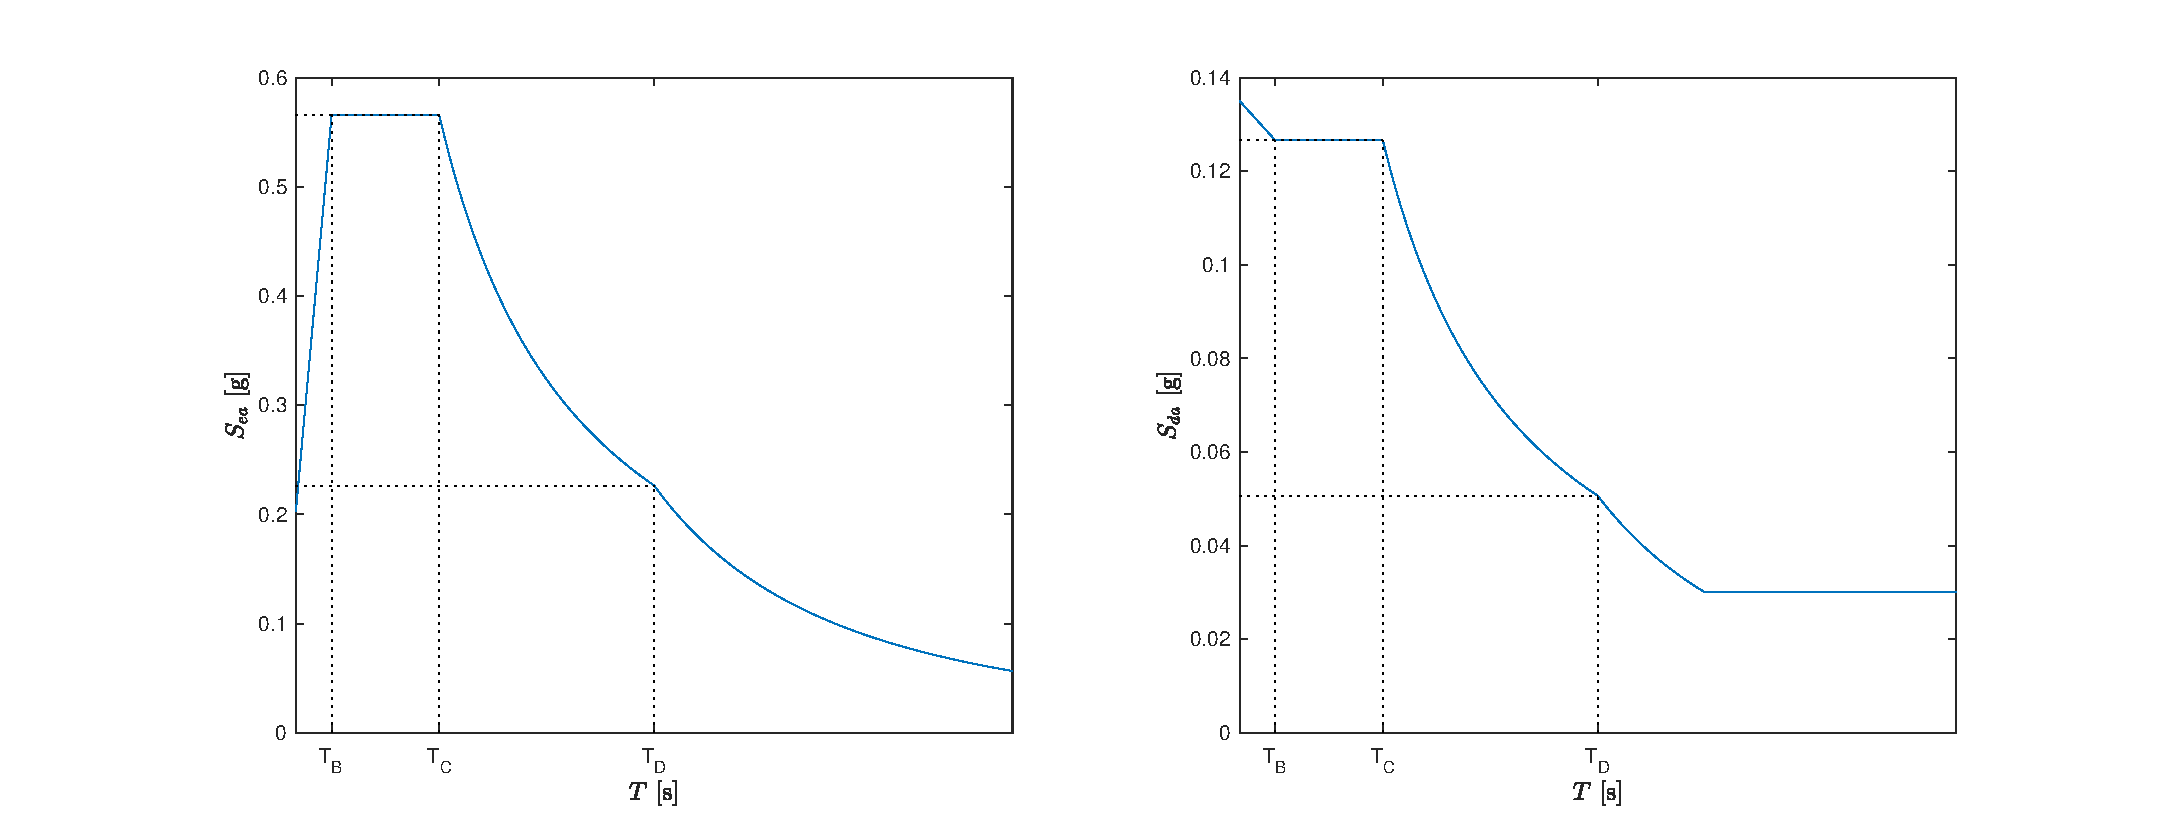
\includegraphics[width=16cm]{Elastic_and_Design_Spectrum.eps}
    \caption{Elastic Spectrum in Right Plot, Design Spectrum in Left Plot}
    \label{fig:I.2: LR - Elastic and Design Spectrum }
\end{figure}
\paragraph{}Both the elastic spectrum, $S_{ea}$, and design spectrum, $S_{da}$, shown above are then used to determine the spectral acceleration relative to the excitation periods of the structure. These plots also show the low branch, constant acceleration branch, constant velocity branch, and constant displacement branch, denoted by the area before $T_B$, the area between $T_B$ and $T_C$, the area between $T_C$ and $T_D$, and the area after $T_D$. The pseudo spectral acceleration relative to the excitation periods of the structure are determined from these plots and are shown in \textsc{Figure}\,\ref{fig:I.2 - LR - spectral accelerations}.
\begin{figure}
    \centering
    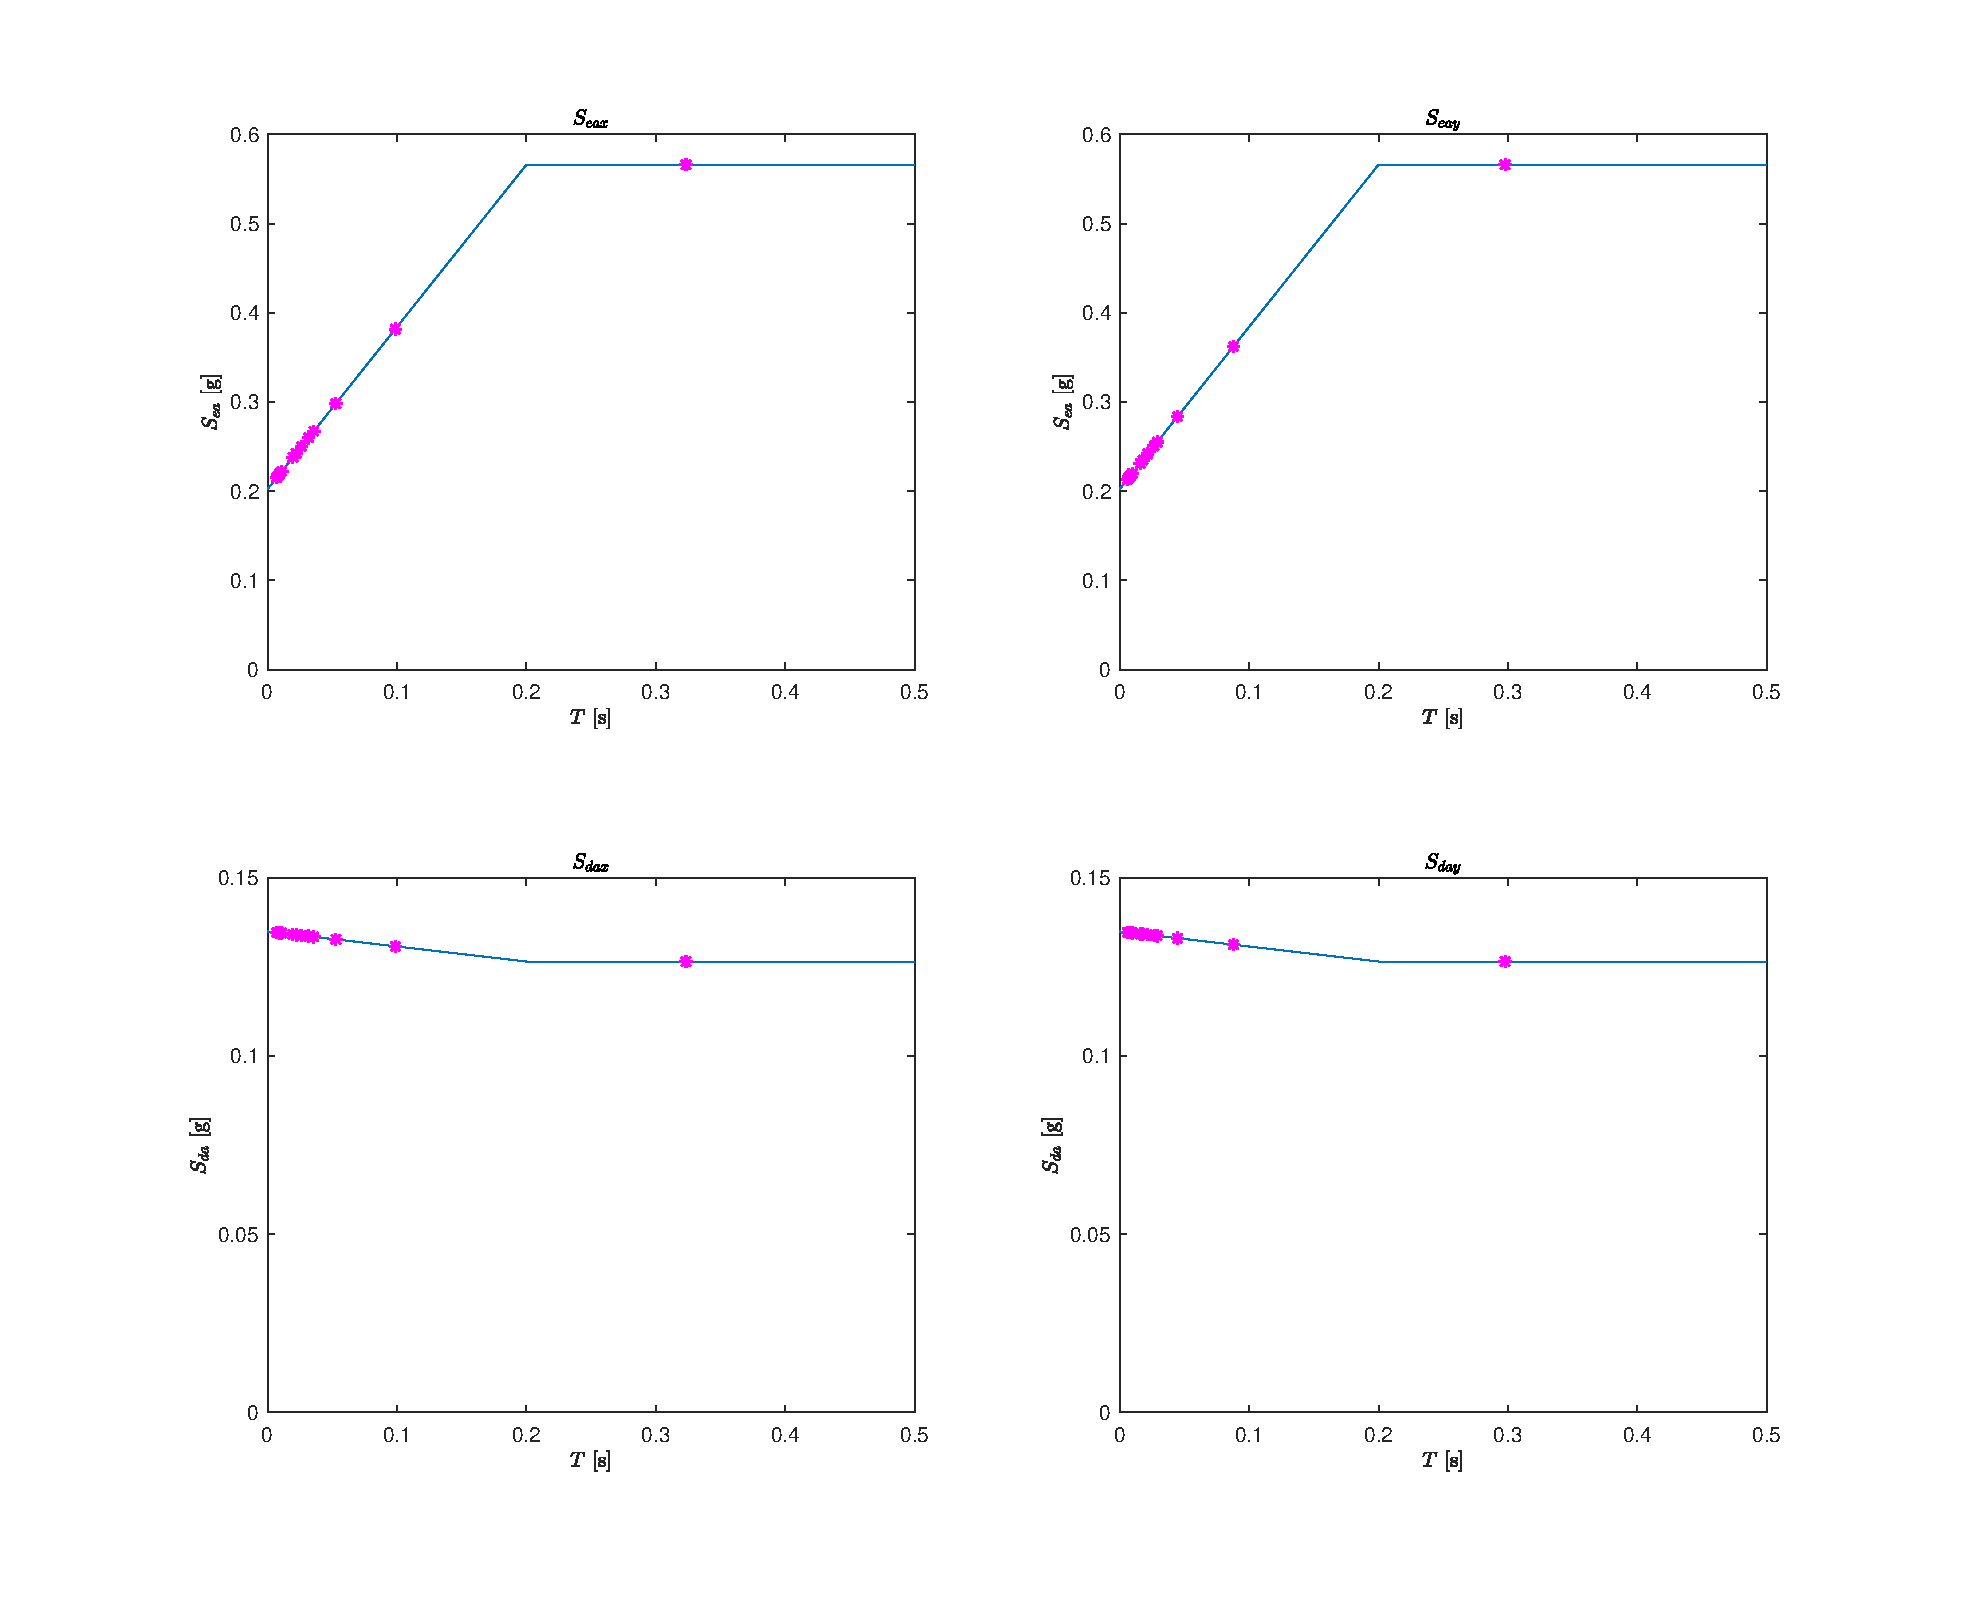
\includegraphics[width=16cm]{Spectral_Accelerations_and_Displacements.eps}
    \caption{Pseudo Spectral Accelerations of the Low Rise Building, top left: elastic spectral accelerations in the (X,Z) plane, top right: elastic spectral accelerations in the (Y,Z) plane, bottom left: design spectral accelerations in the (X,Z) plane, bottom right: design spectral accelerations in the (Y,Z) plane,}
    \label{fig:I.2 - LR - spectral accelerations}
\end{figure}
\subsubsection{Design Displacements}
\paragraph{}The natural period, given by the largest excitation period produces the highest response spectrum. After obtaining this value, the spectral displacements can be derived from their respective spectral accelerations using \textsc{Equation}\,\eqref{eq:I.2 - spectral displacements} below \cite{EC8}. 
\begin{equation}
    S_d = S_a(T_i)\,\omega_i^2\,g
    \label{eq:I.2 - spectral displacements}
\end{equation}
\paragraph{}Where,
\begin{itemize}
\begin{small}
    \item $S_a(T_i)$ is the pseudo spectral acceleration relative to the mode $i$ $[g]$
    \item $\omega_i$ is the angular frequency relative to mode $i$ $[rad/s]$
    \item $g$ is the acceleration due to gravity $[m/s^2]$
\end{small}
\end{itemize}
\subsubsection{Elastic Displacements}
\paragraph{} Using the elastic spectrum produced in \textsc{Equation}\,\eqref{eq:I.2 - Low Rise - Elastic Spectrum} the elastic displacements, $S_{e,d}$, of the structure are determined from  \textsc{Equation}\,\eqref{eq:I.2 - Low Rise - Elastic Spectrum Displacement} below \cite{EC8}.
\begin{equation}
    S_{e,d} = S_{e,a}(T_i)\left[\dfrac{T_i^2}{4\,\pi^2}\right]
    \label{eq:I.2 - Low Rise - Elastic Spectrum Displacement}
\end{equation}
\paragraph{}Where,
\begin{itemize}
\begin{small}
    \item $S_{e,a}$ is the elastic spectrum determined in \textsc{Equation}\,\eqref{eq:I.2 - Low Rise - Elastic Spectrum Displacement} 
    \item $T_i$ is the period of the mode of the specific element  $(i = 1,2,...,12)$ $[s]$
\end{small}
\end{itemize}
\subsection{Modal Displacements}\label{sec: Low Rise - Modal Displacmenets}
\paragraph{}The derivation of the modal elastic displacements, $U_i$, in the low rise building is provided in \textsc{Equation}\,\eqref{eq:I.2 Low Rise - Total Elastic Displacement} below. This determines the peak response of mode $i$, it is unknown where in time this peak value will occur \cite{EC8}. 
\begin{equation}
    U_{i,e}=MPF_i\,\phi_i\,S_{e,d}
    \label{eq:I.2 Low Rise - Total Elastic Displacement}
\end{equation}
\paragraph{}To determine the design modal displacements a similar equation is used and is given by
\begin{equation}
    U_{i,d} = MPF_i\,\phi_i\,S_{d,d}\,q
    \label{eq:I.2: Low Rise - Design Modal Displacments}
\end{equation}
\paragraph{}Where,
\begin{itemize}
\begin{small}
    \item $MPF_i$ is the modal participation factor for a specific mode, $(i = 1,2,...,12)$ given in \textsc{Equation}\,\eqref{eq:I.1 - Modal Participation Factor - High Rise} $[-]$
    \item $\phi_i$ is the mode shape $(i = 1,2,...,12)$  given in \textsc{Equation}\,\eqref{eq: I.1 - function of the eigenmodes} $[-]$
    \item $S_{e,d}$ is the spectral elastic displacement determined in \textsc{Equation}\,\eqref{eq:I.2 - Low Rise - Elastic Spectrum} $[m]$
    \item $q$ is the behavioral factor (in which the damping ratio of the structure is already taken into account) for the low rise building found in \textsc{Table}\,\ref{tab: Specifications - Design LowRB } $[-]$
\end{small}
\end{itemize}
\paragraph{}It should be noted, that to find the design modal displacements within the (X,Z) or (Y,Z) planes that the parameters explained above must be used from the respective (X,Z) and (Y,Z). Additionally the behavioral factor must be applied to this equation to find the true displacement of the structure. 
\begin{table}[h]
    \centering
    \begin{tiny}
    \begin{array}{c|c|c|c|c|c|c|c|c|c|c|c|c|c}
        DOF & Unit & Mode\,1 & Mode\,2 & Mode\,3 & Mode\,4 & Mode\,5 & Mode\,6 & Mode\,7 & Mode\,8 & Mode\,9 & Mode\,10 & Mode\,11 & Mode\,12\\
        \hline 
       1 & $[m]$ & 4.3$x${10}^{-3} & 2.8$x${10}^{-4} & 5.5$x${10}^{-5} & 1.1$x${10}^{-5} & 2.3$x${10}^{-35} & -1.6$x${10}^{-37} & -1.1$x${10}^{-36} & -2.5$x${10}^{-37} & 1.6$x${10}^{-8} & 1.4$x${10}^{-8} & -5.2$x${10}{-9} & -2.6$x${10}^{-9}\\
       2 & $[rad/s]$ & -2.0$x${10}^{-3} & -9.1$x${10}^{-5} & -4.3$x${10}^{-6} & 2.9$x${10}^{-6} & -1.3$x${10}^{-20} & 7.4$x${10}^{-21} & -1.2$x${10}^{-20} & 5.8$x${10}^{-21} & 1.7$x${10}^{-7} & 4.6$x${10}^{-7} & 2.5$x${10}^{-7} & 5.4$x${10}^{-8}\\ 
       3 & $[rad/s]$ & -2.0$x${10}^{-3} & -9.1$x${10}^{-5} & -4.3$x${10}^{-6} & 2.9$x${10}^{-6} & 1.3$x${10}^{-20} & -7.4$x${10}^{-21} & 1.2$x${10}^{-20} & -5.8$x${10}^{-21} & 1.7$x${10}^{-7} & 4.6$x${10}^{-7} & 2.5$x${10}^{-7} & 5.4$x${10}^{-8}\\
       4 & $[m]$ & 0.011 & 3.9$x${10}^{-4} & -2.3$x${10}^{-6} & -1.3$x${10}^{-5} & -4.9$x${10}^{-35} & 2.0$x${10}^{-36} & -1.6$x${10}^{-36} & 1.3$x${10}^{-36} & -1.2$x${10}^{-8} & 2.5$x${10}^{-8} & 1.4$x${10}^{-8} & -1.1$x${10}^{-9}\\
       5 & $[rad/s]$ & -1.9$x${10}^{-3} & 4.4$x${10}^{-5} & 2.6$x${10}^{-5} & 3.6$x${10}^{-7} & 2.7$x${10}^{-20} & -7.9$x${10}^{-21} & -4.4$x${10}^{-21} & 8.9$x${10}^{-21} & -3.0$x${10}^{-7} & -3.7$x${10}^{-7} & 1.4$x${10}^{-7} & 9.1$x${10}^{-8}\\
       6 & $[rad/s]$ & -1.9$x${10}^{-3} & 4.4$x${10}^{-5} & 2.6$x${10}^{-5} & 3.6$x${10}^{-7} & -2.7$x${10}^{-20} & 7.9$x${10}^{-21} & 4.4$x${10}^{-21} & -8.9$x${10}^{-21} & -3.0$x${10}^{-7} & -3.7$x${10}^{-7} & 1.4$x${10}^{-7} & 9.1$x${10}^{-8}\\ 
       7 & $[m]$ & 0.016 & 3.2$x${10}^{-5} & -5.0$x${10}^{-5} & 9.8$x${10}^{-6} & 1.4$x${10}^{-34} & 3.7$x${10}^{-36} & 3.5$x${10}^{-36} & 1.1$x${10}^{-36} & 6.2$x${10}^{-9} & -3.7$x${10}^{-8} & 1.2$x${10}^{-8} & 9.3$x${10}^{-10}\\
       8 & $[rad/s]$ & -1.3$x${10}^{-3} & 1.5$x${10}^{-4} & -9.5$x${10}^{-6} & -3.1$x${10}^{-6} & -4.5$x${10}^{-20} & 1.1$x${10}^{-21} & 1.1$x${10}^{-20} & 8.1$x${10}^{-21} & 3.8$x${10}^{-7} & -1.1$x${10}^{-7} & -1.8$x${10}^{-7} & 9.3$x${10}^{-8}\\ 
       9 & $[rad/s]$ & -1.3$x${10}^{-3} & 1.5$x${10}^{-4} & -9.5$x${10}^{-6} & -3.1$x${10}^{-6} & 4.5$x${10}^{-20} & -1.1$x${10}^{-21} & -1.1$x${10}^{-20} & -8.1$x${10}^{-21} & 3.8$x${10}^{-7} & -1.1$x${10}^{-7} & -1.8$x${10}^{-7} & 9.3$x${10}^{-8}\\ 
       10 & $[m]$ & 0.019 & -4.1$x${10}^{-4} & 4.3$x${10}^{-5} & -5.0$x${10}^{-6} & -6.8$x${10}^{-35} & -4.8$x${10}^{-36} & 7.6$x${10}^{-36} & 3.8$x${10}^{-36} & 1.7$x${10}^{-8} & -8.0$x${10}^{-10} & -7.4$x${10}^{-9} & 2.9$x${10}^{-9}\\
       11 & $[rad/s]$ & -6.2$x${10}^{-4} & 1.1$x${10}^{-4} & -2.9$x${10}^{-5} & 6.2$x${10}^{-6} & 6.9$x${10}^{-20} & 6.8$x${10}^{-21} & 8.2$x${10}^{-21} & 3.7$x${10}^{-21} & -4.2$x${10}^{-7} & 4.9$x${10}^{-7} & -2.3$x${10}^{-7} & 5.7$x${10}^{-8}\\ 
        12 & $[rad/s]$ & -6.2$x${10}^{-4} & 1.1$x${10}^{-4} & -2.9$x${10}^{-5} & 6.2$x${10}^{-6} & -6.9$x${10}^{-20} & -6.8$x${10}^{-21} & -8.2$x${10}^{-21} & -3.7$x${10}^{-21} & -4.2$x${10}^{-7} & 4.9$x${10}^{-7} & -2.3$x${10}^{-7} & 5.7$x${10}^{-8} \\
    \end{array}
    \caption{Modal Elastic Displacement in the (X,Z) plane}
    \label{tab:my_label}
    \end{tiny}
\end{table}
\todo{either delete or appendix}
\begin{table}[h]
    \centering
    \begin{tabular}{c|c|c|c|c|c|c|c|c|c|c|c|c|c}
        DOF & Unit & $1$ & $2$ & $3$ & $4$ & $5$ & $6$ & $7$ & $8$ & $9$ & $10$ & $11$ & $12$\\
        \hline 
        $1$ & $[m]$ & & & & & & & & & & & \\
        $2$ & $[rad]$ & & & & & & & & & & & \\
        $3$ & $[rad]$ & & & & & & & & & & & \\
        $4$ & $[m]$ & & & & & & & & & & & \\
        $5$ & $[rad]$ & & & & & & & & & & & \\
        $6$ & $[rad]$ & & & & & & & & & & & \\
        $7$ & $[m]$ & & & & & & & & & & & \\
        $8$ & $[rad]$ & & & & & & & & & & & \\
        $9$ & $[rad]$ & & & & & & & & & & & \\
        $10$ & $[m]$ & & & & & & & & & & & \\
        $11$ & $[rad]$ & & & & & & & & & & & \\
        $12$ & $[rad]$ & & & & & & & & & & & \\
    \end{tabular}
    \caption{Modal Elastic Displacement in the (Y,Z) plane}
    \label{tab:my_label}
\end{table}
\begin{table}[h]
    \centering
    \begin{tabular}{c|c|c|c|c|c|c|c|c|c|c|c|c|c}
        DOF & Unit & $1$ & $2$ & $3$ & $4$ & $5$ & $6$ & $7$ & $8$ & $9$ & $10$ & $11$ & $12$\\
        \hline 
        $1$ & $[m]$ & & & & & & & & & & & \\
        $2$ & $[rad]$ & & & & & & & & & & & \\
        $3$ & $[rad]$ & & & & & & & & & & & \\
        $4$ & $[m]$ & & & & & & & & & & & \\
        $5$ & $[rad]$ & & & & & & & & & & & \\
        $6$ & $[rad]$ & & & & & & & & & & & \\
        $7$ & $[m]$ & & & & & & & & & & & \\
        $8$ & $[rad]$ & & & & & & & & & & & \\
        $9$ & $[rad]$ & & & & & & & & & & & \\
        $10$ & $[m]$ & & & & & & & & & & & \\
        $11$ & $[rad]$ & & & & & & & & & & & \\
        $12$ & $[rad]$ & & & & & & & & & & & \\
    \end{tabular}
    \caption{Modal Design Displacement in the (X,Z) plane}
    \label{tab:my_label}
\end{table}
\begin{table}[h]
    \centering
    \begin{tabular}{c|c|c|c|c|c|c|c|c|c|c|c|c|c}
        DOF & Unit & $1$ & $2$ & $3$ & $4$ & $5$ & $6$ & $7$ & $8$ & $9$ & $10$ & $11$ & $12$\\
        \hline 
        $1$ & $[m]$ & & & & & & & & & & & \\
        $2$ & $[rad]$ & & & & & & & & & & & \\
        $3$ & $[rad]$ & & & & & & & & & & & \\
        $4$ & $[m]$ & & & & & & & & & & & \\
        $5$ & $[rad]$ & & & & & & & & & & & \\
        $6$ & $[rad]$ & & & & & & & & & & & \\
        $7$ & $[m]$ & & & & & & & & & & & \\
        $8$ & $[rad]$ & & & & & & & & & & & \\
        $9$ & $[rad]$ & & & & & & & & & & & \\
        $10$ & $[m]$ & & & & & & & & & & & \\
        $11$ & $[rad]$ & & & & & & & & & & & \\
        $12$ & $[rad]$ & & & & & & & & & & & \\
    \end{tabular}
    \caption{Modal Design Displacement in the (Y,Z) plane}
    \label{tab:my_label}
\end{table}

\paragraph{}The modal displacements derived show that the elastic displacement results are larger than the design displacements in the (X,Z) plane, but in the (Y,Z) plane the design displacements are larger than the elastic displacements. This is potentially a result of a higher deviation in results of the elastic displacements than that of the design displacements. As, for both the elastic and design the displacements are larger in the (X,Z) plane than the (Y,Z) plane.
\subsection{Total Displacements}\label{sec: Low Rise - Total Displacements}
\paragraph{}To determine total displacements of the low rise building two different modal combination rules have been used. These are the square root of sum of squares (SRSS) method, and the complete quadratic combination (CQC) method.
\subsubsection{Square Root of Sum of Squares - SRSS}
\paragraph{} To determine the peak response of a degree of freedom, the SRSS method takes the summation of the square root of the peak modal response of each mode affecting this degree of freedom. The SSRS method presented in \textsc{Equation}\,\eqref{eq:I.2 - Low Rise - SSRS} shows the derivation for the total displacement, $U_{tot}$, of the low rise building \cite{textbook}.
\begin{equation}
    U_{SRSS} = \sqrt{\sum^N_{n=1}\,U_n\,^2}
    \label{eq:I.2 - Low Rise - SSRS}
\end{equation}
\paragraph{}Where,
\begin{itemize}
\begin{small}
    \item $U_n$ is the modal displacement of mode $i$, at the studied DOF
    \item $N$ is the number of modes considered in the structures analysis $(N=1,2,...,12)$
\end{small}
\end{itemize}
\subsubsection{Complete Quadratic Combination - CQC}
\paragraph{}The CQC method accounts for more than just the sum of the displacements like that of the SSRS method explained previously. The CQC method determines the total displacement of a degree of freedom within the structure by obtaining the peak response at each mode of the degree of freedom and correlating these modal responses with the correlation factor, $\rho_{in}$. The correlation factor is a product of the damping properties of the structure and the frequency ratio between the two modes. The correlation coefficient is a measure of correlation between modes $i$ and $n$. The derivation of the correlation coefficient is seen in \textsc{Equation}\,\eqref{eq:I.2 - Low Rise - Correlation Coefficient} \cite{textbook}.
\begin{equation}
    \rho_{in}=\dfrac{8\,\xi^2\,(1+\beta_{in})\,\beta_{in}^{3/2}}{(1-\beta_{in}^2)+4\,\xi^2\,\beta_{in}\,(1+\beta_{in})^2}
    \label{eq:I.2 - Low Rise - Correlation Coefficient}
\end{equation}
\paragraph{}Where,
\begin{itemize}
    \item $\xi$ is damping ratio given in \textsc{Table}\,\ref{tab: Specifications - Design LowRB }
    \item $\beta_{in}$ is the ratio between the angular frequency of mode $i$ and that of mode $n$, called the correlation coefficient $[-]$
\end{itemize}
\paragraph{}Now that the correlation coefficient and its dependent variables have been determined, the total displacement at a specified DOF of the structure, $U_{tot}$, of the structure can be determined with the CQC method as shown in \textsc{Equation}\,\eqref{eq:I.2 - Low Rise - CQC} \cite{textbook}.
\begin{equation}
    U_{CQC} = \sqrt{\sum^N_{n=1}\,\sum^N_{i=1}\,\rho_{in}\,U_i\,U_n}
    \label{eq:I.2 - Low Rise - CQC}
\end{equation}
\paragraph{}Where,
\begin{itemize}
\begin{small}
    \item $\rho_{in}$ is the correlation coefficient determined in \textsc{Equation}\,\eqref{eq:I.2 - Low Rise - Correlation Coefficient}
    \item $U_n$ is the modal displacement of mode $n$ $[m]$
    \item $U_i$ is the modal displacement of mode $i$ $[m]$
    \item $N$ is the number of modes taken into account for the analysis of the structure
\end{small}
\end{itemize}
\paragraph{}The numerical outputs for the total design displacements produced using the CQC method of modal combination. \textsc{Table}\,\ref{tab:total elastic and design displacements X} and  \textsc{Table}\,\ref{tab:total elastic and design displacements Y} below gives the total displacements at each global degree of freedom in the (X,Z) plane and the (Y,Z) plane of the low rise building.
\todo{is this DOF or mode????}
\begin{table}[h]
    \centering
    \begin{tabular}{c|c|c|c|c|c}
         DOF & Unit & $U_{i,e} SRSS [cm]$ & $U_{i,e} CQC [cm]$ & $U_{i,d} SRSS [cm]$ & $U_{i,d} CQC [cm]$\\
         \hline
        $1$ & $[cm]$ & $0.43$ & $0.43$ & $0.39$ & $0.39$ \\
        $2$ & $[rad\,cm]$ & $0.20$ & $0.20$ & $0.18$ & $0.18$ \\
        $3$ & $[rad\,cm]$ &$0.20$ & $0.20$ & $0.18$ & $0.18$ \\
        $4$ & $[cm]$ & $1.08$ & $1.08$ & $0.97$ & $0.97$ \\
        $5$ & $[rad\,cm]$ &$0.19$ & $0.19$ & $0.17$ & $0.17$ \\
        $6$ & $[rad\,cm]$ &$0.19$ & $0.19$ & $0.17$ & $0.17$ \\
        $7$ & $[cm]$ & $1.61$ & $1.61$ & $1.44$ & $1.44$ \\
        $8$ & $[rad\,cm]$ &$0.13$ & $0.13$ & $0.12$ & $0.12$ \\
        $9$ & $[rad\,cm]$ &$0.13$ & $0.13$ & $0.12$ & $0.12$ \\
        $10$ & $[cm]$ & $1.91$ & $1.91$ & $1.71$ & $1.71$ \\
        $11$ & $[rad\,cm]$ &$0.06$ & $0.06$ & $0.06$ & $0.06$ \\
        $12$ & $[rad\,cm]$ &$0.06$ & $0.06$ & $0.06$ & $0.06$ \\
    \end{tabular}
    \caption{Total Elastic and Design Displacements in the (X,Z) plane}
    \label{tab:total elastic and design displacements X}
\end{table}
\begin{table}[h]
    \centering
       \begin{tabular}{c|c|c|c|c|c}
         DOF & Unit & $U_{i,e} SRSS [cm]$ & $U_{i,e} CQC [cm]$ & $U_{i,d} SRSS [cm]$ & $U_{i,d} CQC [cm]$\\
         \hline
        $1$ & $[cm]$ &$ 0.33$ & $ 0.33$ & $0.35$ & $0.35$ \\
        $2$ & $[rad\,cm]$ & $0.17$ & $0.17$ & $0.18$ & $0.18$ \\
        $3$ & $[rad\,cm]$ & $0.17$ & $0.17$ & $0.18$ & $0.18$ \\
        $4$ & $[cm]$ &$0.88$ & $0.88$ & $0.93$ & $0.93$ \\
        $5$ & $[rad\,cm]$ & $0.18$ & $0.18$ & $0.19$ & $0.19$ \\
        $6$ & $[rad\,cm]$ & $0.18$ & $0.18$ & $0.19$ & $0.19$ \\
        $7$ & $[cm]$ &$1.35$ & $1.35$ & $1.42$ & $1.42$ \\
        $8$ & $[rad\,cm]$ & $0.13$ & $0.13$ & $0.14$ & $0.14$ \\
        $9$ & $[rad\,cm]$ & $0.13$ & $0.13$ & $0.14$ & $0.14$ \\
        $10$ & $[cm]$ & $1.64$ & $1.64$ & $1.73$ & $1.73$ \\
        $11$ & $[rad\,cm]$ & $0.07$ & $0.07$ & $0.08$ & $0.08$ \\
        $12$ & $[rad\,cm]$ & $0.07$ & $0.07$ & $0.08$ & $0.08$ \\
    \end{tabular}
    \caption{Total Elastic and Design Displacements in the (Y,Z) plane}
    \label{tab:total elastic and design displacements Y}
\end{table}
\todo{comment that these are really wrong}
\paragraph{} As seen in \textsc{Table}\,\ref{tab:total elastic and design displacements X} and \textsc{Table}\,\ref{tab:total elastic and design displacements Y} the total displacements of the low rise building are larger in the (X,Z) plane than the (Y,Z) plane. As previously discussed in Chapter 2, this is due to the geometry of the building. 
\subsection{Modal Section Forces}\label{sec: Low Rise - Modal Section Forces}
\paragraph{}The modal seismic section forces developing in element $i$ are determined using \textsc{Equation}\,\eqref{eqI.2 Low Rise - Modal Section Forces}. The section forces of the low rise building will be calculated using the design spectrum because, for the low rise building the behavioral factor, $q$, is not equal to 1. This is because it is a statistically indeterminate structure, so that it is able to exhibit plastic deformation before it fails. The $q$ factor accounts for the difference between the elastic spectrum and the design spectrum. The elastic spectrum is used for statistically determinate structure, where if any plastic deformation occurs, the entire structure fails. If the elastic spectrum is used for a statistically indeterminate building, the structure will be over designed. For this reason, the design spectrum is used to calculate its section forces for the low rise building. Since the seismic forces (represented by the acceleration spectrum) are horizontal forces only, in the analysis only uses the horizontal spectrum. As previously stated it is assumed that the acceleration is only in the horizontal direction. The results of the modal section forces have been provided in \textsc{Appendix}\ref{sec: appendix A}
\begin{equation}
   \left[
   \begin{matrix}
   F_1\\
   F_2\\
   M_3\\
   M_4\\
   \end{matrix}
   \right] = K_i
     \left[
   \begin{matrix}
   u_1\\
   u_2\\
   u_3\\
   u_4\\
   \end{matrix}
   \right]
   \label{eqI.2 Low Rise - Modal Section Forces}
\end{equation}
\paragraph{}Where,
\begin{itemize}
    \item $F_1$ and $F_2$ are the shear forces at the two extreme ends of the element $i$ as shown in \textsc{Figure}\,\ref{fig : I.1 - local axis LowRB} $[N]$
    \item $F_3$ and $F_4$ are the bending moments at the twp extreme ends of the element $i$ as shown in \textsc{Figure}\,\ref{fig : I.1 - local axis LowRB} $[Nm]$
    \item $K_i$ is the local stiffness matrix of element $i$ $[N]$
    \item $u_1$ and $u_2$ are the resulting displacements $[m]$
    \item $u_3$ and $u_4$ are the resulting rotations $[rad]$
\end{itemize}
\subsection{Total Section Forces}\label{sec: Low Rise - Total Section Forces}
\paragraph{} The total seismic section forces acting on the building are determined using the same modal combination methods used to determine the modal displacements. This is determined using the same SRSS and CQC methods used to determine the total displacements as described previously. The results of these combinations in the (X,Z) and (Y,Z) planes can be seen in \textsc{Table}\,\ref{tab:totl section forces SRSS X}, \ref{tab:totl section forces SRSS Y}, \ref{tab:totl section forces CQC X}, and \ref{tab:totl section forces CQC Y}.
\begin{table}[h]
    \centering
    \begin{tabular}{c|c|c|c|c}
    Element & $F_1 [kN]$ & $F_2 [kN]$ & $M_3 [kNm]$ & $M_4 [kNm]$ \\
    \hline
       $1$ & $28.7736$ & $28.7736$ & $ 20.1057$ & $51.8939$ \\
       $2$ & $ 25.8105$ & $25.8105$ & $32.5528$ & $32.0669$ \\
       $3$ & $19.2396$ & $19.2396$ & $29.0070$ & $19.2723$ \\
       $4$ & $9.5897$ & $9.5897$ & $17.3987$ & $6.9125$ \\
       $5$ & $ 9.5897 $ & $9.5897$ & $17.3987$ & $ 6.9125$ \\
       $6$ & $19.2396$ & $19.2396$ & $29.0070$ & $19.2723$ \\
       $7$ & $25.8105$ & $25.8105$ & $32.5528$ & $32.0669$ \\
       $8$ & $ 28.7736$ & $28.7736$ & $20.1057$ & $51.8939$ \\
       $9$ & $23.1021$ & $23.1021$ & $51.9797$ & $51.9797$ \\
       $10$ & $22.7929$ & $22.7929$ & $51.2840$ & $51.2840$ \\
       $11$ & $ 15.6032 $ & $ 15.6032 $ & $35.1072$ & $35.1072$ \\
       $12$ & $ 7.5820$ & $ 7.5820$ & $17.0595$ & $17.0595$ \\
    \end{tabular}
    \caption{Total Section Forces using SRSS Combination in the (X,Z) plane}
    \label{tab:totl section forces SRSS X}
\end{table}
\begin{table}[h]
    \centering
    \begin{tabular}{c|c|c|c|c}
    Element & $F_1 [kN]$ & $F_2 [kN]$ & $M_3 [kNm]$ & $M_4 [kNm]$ \\
    \hline
       $1$ & $33.4537$ & $33.4537$ & $16.1543$ & $67.7921$ \\
       $2$ & $30.1215$ & $30.1215$ & $36.6952$ & $38.8530$ \\
       $3$ & $22.6832$ & $22.6832$ & $35.9534$ & $21.2531$ \\
       $4$ & $11.5906$ & $11.5906$ & $22.9954$ & $7.1735$ \\
       $5$ & $11.5906$ & $11.5906$ & $22.9954$ & $7.1735$ \\
       $6$ & $22.6832$ & $22.6832$ & $35.9534$ & $21.2531$ \\
       $7$ & $30.1215$ & $30.1215$ & $36.6952$ & $38.8530$ \\
       $8$ & $33.4537$ & $33.4537$ & $16.1543$ & $67.7921$ \\
       $9$ & $24.1398$ & $24.1398$ & $54.3145$ & $54.3145$ \\
       $10$ & $25.2138$ & $25.2138$ & $56.7309$ & $56.7309$ \\
       $11$ & $18.1904$ & $18.1904$ & $40.9284$ & $40.9284$ \\
       $12$ & $10.0509$ & $10.0509$ & $22.6144$ & $22.6144$ \\
    \end{tabular}
    \caption{Total Section Forces using SRSS Combination in the (Y,Z) plane}
    \label{tab:totl section forces SRSS Y}
\end{table}
\begin{table}[h]
    \centering
    \begin{tabular}{c|c|c|c|c}
    Element & $F_1 [kN]$ & $F_2 [kN]$ & $M_3 [kNm]$ & $M_4 [kNm]$ \\
    \hline
       $1$ & $28.7848$ & $28.7848$ & $20.1189$ & $51.9096$ \\
       $2$ & $25.8120$ & $25.8120$ & $32.5576$ & $32.0662$ \\
       $3$ & $19.2341$ & $19.2341$ & $29.0019$ & $19.2633$ \\
       $4$ & $9.5800$ & $9.5800$ & $17.3878$ & $6.8960$ \\
       $5$ & $9.5800$ & $9.5800$ & $17.3878$ & $6.8960$ \\
       $6$ & $19.2341$ & $19.2341$ & $29.0019$ & $19.2633$ \\
       $7$ & $ 25.8120$ & $25.8120$ & $32.5576$ & $32.0662$ \\
       $8$ & $28.7848$ & $28.7848$ & $20.1189$ & $51.9096$ \\
       $9$ & $23.1053$ & $23.1053$ & $51.9869 $ & $51.9869$ \\
       $10$ & $22.7912$ & $22.7912$ & $51.2802$ & $51.2802$ \\
       $11$ & $15.5981$ & $15.5981$ & $35.0957$ & $35.0957$ \\
       $12$ & $7.5771$ & $7.5771 $ & $17.0484$ & $17.0484$ \\
    \end{tabular}
    \caption{Total Section Forces using CQC Combination in the (X,Z) plane}
    \label{tab:totl section forces CQC X}
\end{table}
\begin{table}[h]
    \centering
    \begin{tabular}{c|c|c|c|c}
    Element & $F_1 [kN]$ & $F_2 [kN]$ & $M_3 [kNm]$ & $M_4 [kNm]$ \\
    \hline
       $1$ & $33.4687$ & $33.4687$ & $16.1741$ & $67.8135$ \\
       $2$ & $30.1240$ & $30.1240$ & $36.7028$ & $38.8522$ \\
       $3$ & $22.6767$ & $22.6767$ & $35.9483$ & $21.2414$ \\
       $4$ & $11.5783$ & $11.5783$ & $22.9829$ & $7.1477$ \\
       $5$ & $11.5783$ & $11.5783$ & $22.9829$ & $7.1477$ \\
       $6$ & $22.6767$ & $22.6767$ & $35.9483$ & $21.2414$ \\
       $7$ & $30.1240$ & $30.1240$ & $36.7028$ & $38.8522$ \\
       $8$ & $33.4687$ & $33.4687$ & $16.1741$ & $67.8135$ \\
       $9$ & $24.1432$ & $24.1432$ & $54.3223$ & $54.3223$ \\
       $10$ & $25.2122 $ & $25.2122 $ & $ 56.7275 $ & $ 56.7275 $ \\
       $11$ & $18.1850$ & $18.1850$ & $ 40.9163 $ & $ 40.9163 $ \\
       $12$ & $ 10.0452$ & $ 10.0452$ & $22.6016$ & $22.6016$ \\
    \end{tabular}
    \caption{Total Section Forces using CQC Combination in the (Y,Z) plane}
    \label{tab:totl section forces CQC Y}
\end{table}
\paragraph{}The results of the total section forces for both the (X,Z) and (Y,Z) planes showed larger values when combined using the CQC method rather than the SRSS combination method as expected. The resultant forces produced from the strong ground motions are larger in the (Y,Z) plane than the (X,Z) plane. The following observations are the same in both the (X,Z) and (Y,Z) planes. It can be seen that the forces in the columns are uniform among columns on the same storey with equal shear forces and different moments as expected. The results for the beams show equal shear forces and bending moments at either end of the beam, and decreasing values as the storey increases, as expected. 
\todo{Why bigger in Y???}
\section{High Rise Building}
\paragraph{}The modal response of the high rise building has been analyzed in both the (X,Z) and (Y,Z) directions. The elastic and inelastic response of the structure is analyzed with the horizontal elastic response spectrum and the horizontal design response spectrum, respectively. The elastic spectrum will be used to determine the modal elastic displacements and the total elastic displacements. The design spectrum will be used to determine the modal design displacements, the total design displacements, as well as the modal section forces, and total section forces. This differs from the low rise building as only ofur modes were studied, and the building acts as a continuous system rather than a discrete system like that of the low rise. 

\subsection{Acceleration Spectrums}
\paragraph{}The determination of the elastic modal displacements for the high rise building is the same as that for the low rise building, as described in \textsc{Section}\,\ref{sec: Elastic Modal Displacmenets}. The difference for the high rise building is a change in the damping ratio correction factor, $\eta$. This value is different for the high rise building, as it uses the specific critical damping, $\xi$, of the high rise building, as given in \textsc{Table}\,\ref{tab: Specifications - Design HighRB}. The design displacements for the high rise building are also determined in the same way as for the low rise building as outlined in \textsc{Section}\,\ref{sec: Design Displacements}. The high rise building uses a different behavioral factor, $q$, as given in \textsc{Table}\,\ref{tab: Specifications - Design HighRB}. The results of the elastic and design acceleration spectrum are shown in \textsc{Figure}\,\ref{fig:I.2 - acceleration spectrum HR}. 
\begin{figure}
    \centering
    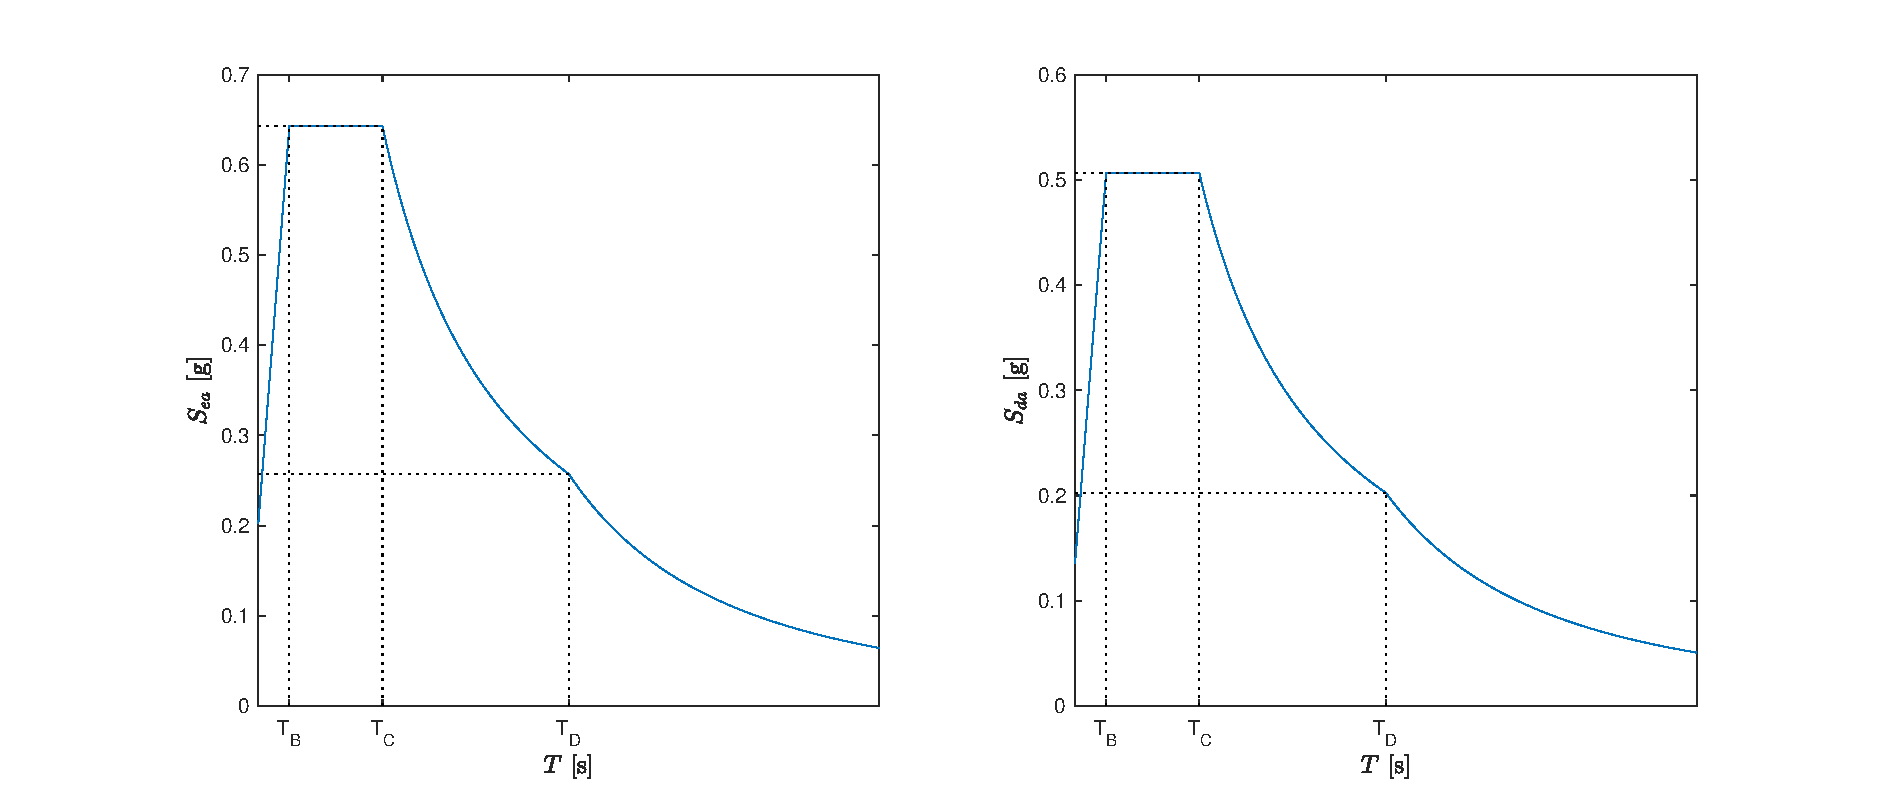
\includegraphics[width=16cm]{Acceleration_Spectrum_HR.eps}
    \caption{Elastic and Design Acceleration Spectrums of the High Rise Building}
    \label{fig:I.2 - acceleration spectrum HR}
\end{figure}
\paragraph{}For the displacement produced from the design spectrum it should be noted that the results produced from this spectrum are made slightly less accurate due to the behavior factor. This is because for the high rise building the behavior factor is equal to 1. A behavior factor of 1 accounts for a structural damping of $5\%$, while in reality the high rise building has a structural damping of $1.2\%$. This means that the actual response of the high rise building would be 4-5 times larger than that of the response produced from the design spectrum. 
 
\subsection{Spectral Displacements}
\paragraph{}The determination of the spectral displacements for the high rise building is the same as that of the low rise building as both structures have a finite number of modes. The determination described in \textsc{Section}\,\ref{sec:low rise spectral displacements} can therefore be followed for the high rise building. The difference for the high rise building is that the amount of specific modes changes to $(i=1,2,3,4)$.
\begin{figure}
    \centering
    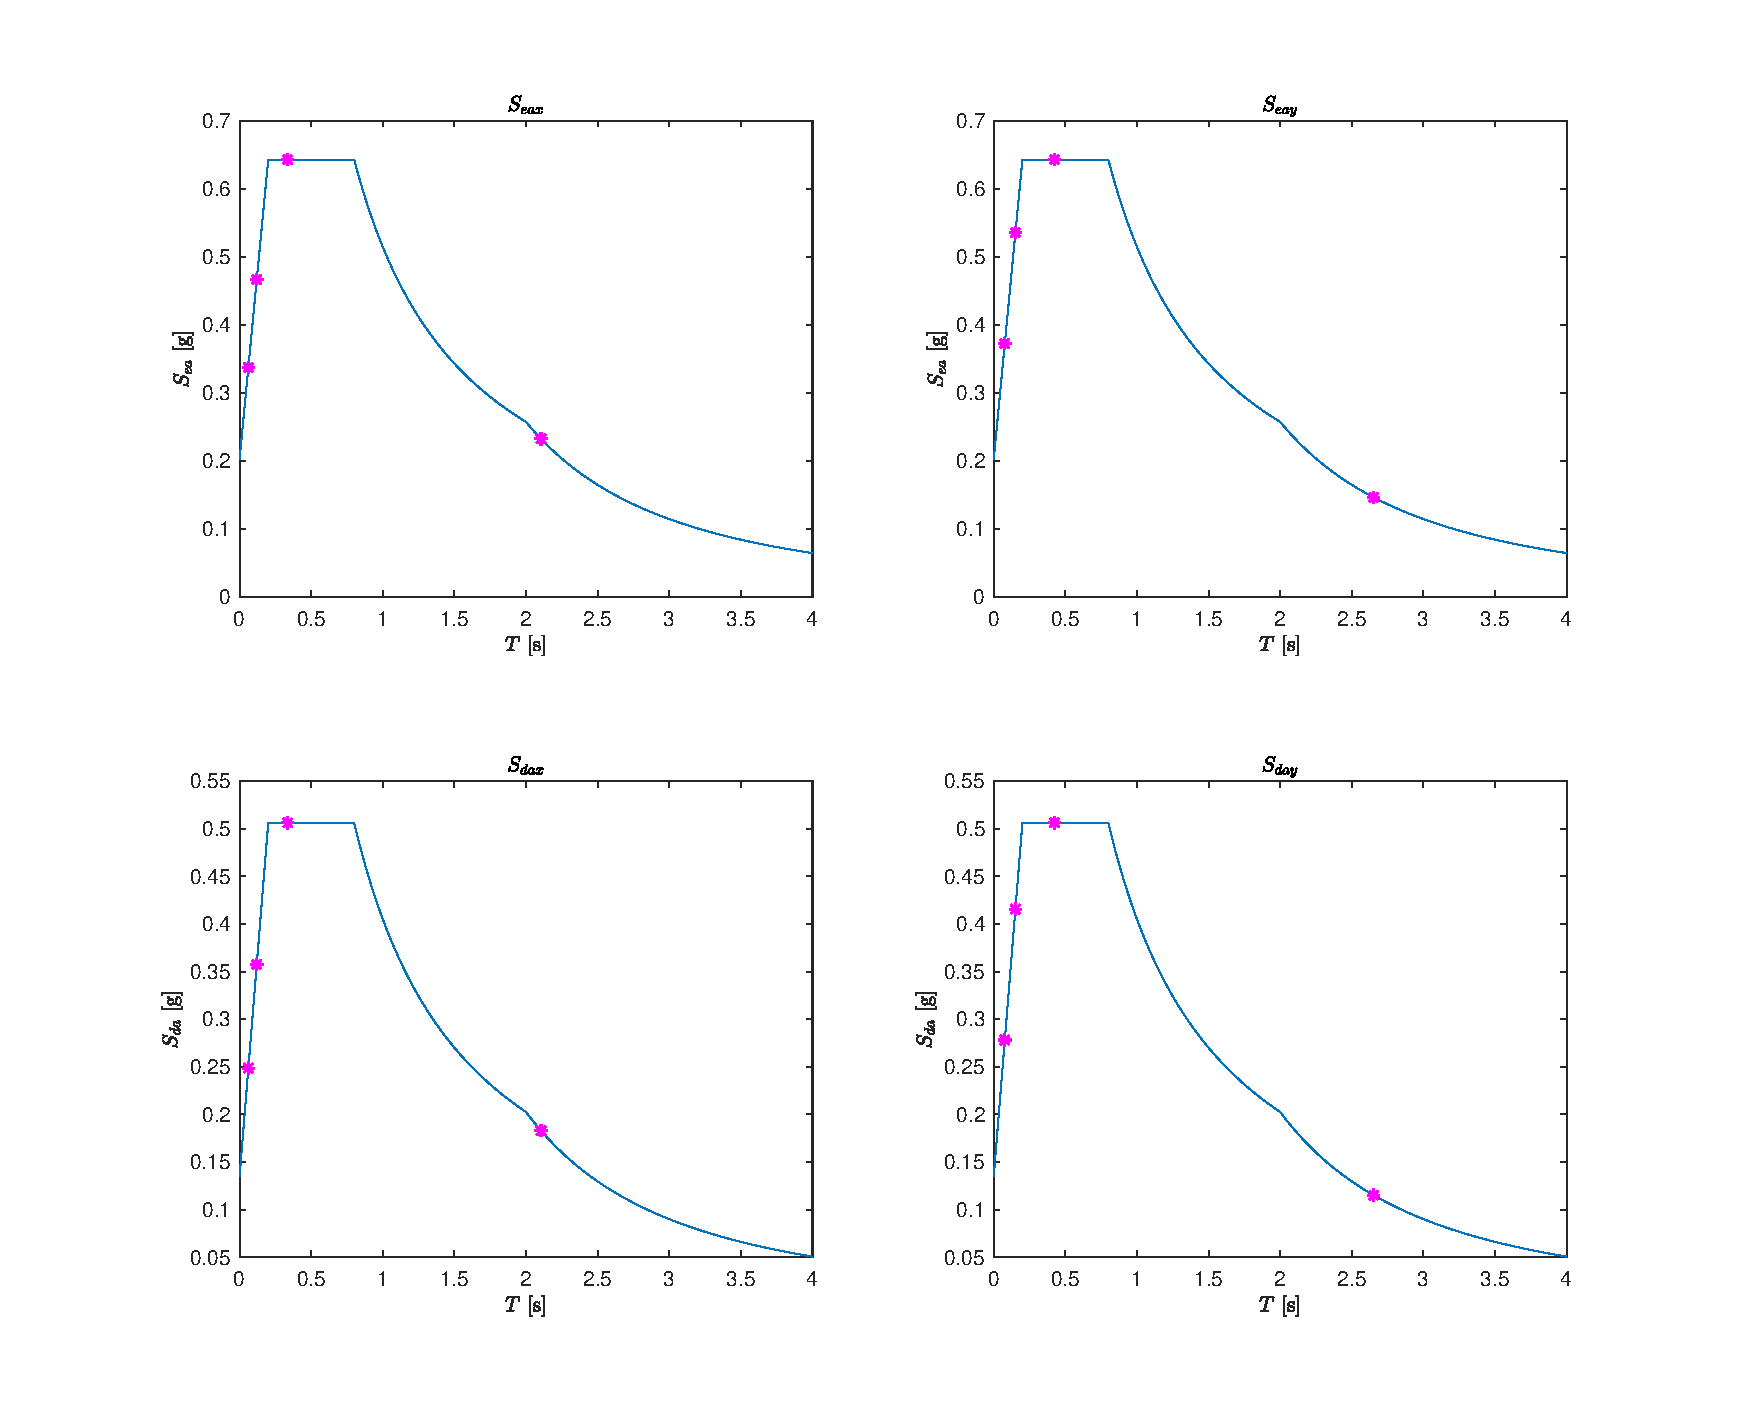
\includegraphics[width=16cm]{Spectral_Displacements_HR.eps}
    \caption{Elastic and Design Spectral Accelerations}
    \label{fig:my_label}
\end{figure}
\subsection{Modal Displacements}
\paragraph{}The modal displacements within the high rise buildling follow the same methods as the low rise building outlined in \textsc{Section}\,\ref{sec: Low Rise - Modal Displacmenets}. The results shown in \textsc{Figure}\,\ref{fig:I.2 Modal Displacements HR} show the displacements of each mode from the elastic spectrum and design spectrum in both the (X,Z) plane and (Y,Z) plane. It should be noted that these figures show increasing horizontal exaggeration as the mode number increases. While it appears the displacements are quite similar for each mode shape, they in fact are not as their displacements are related to their modal participation factor, which decreases significantly with mode number.
\begin{figure}
    \centering
    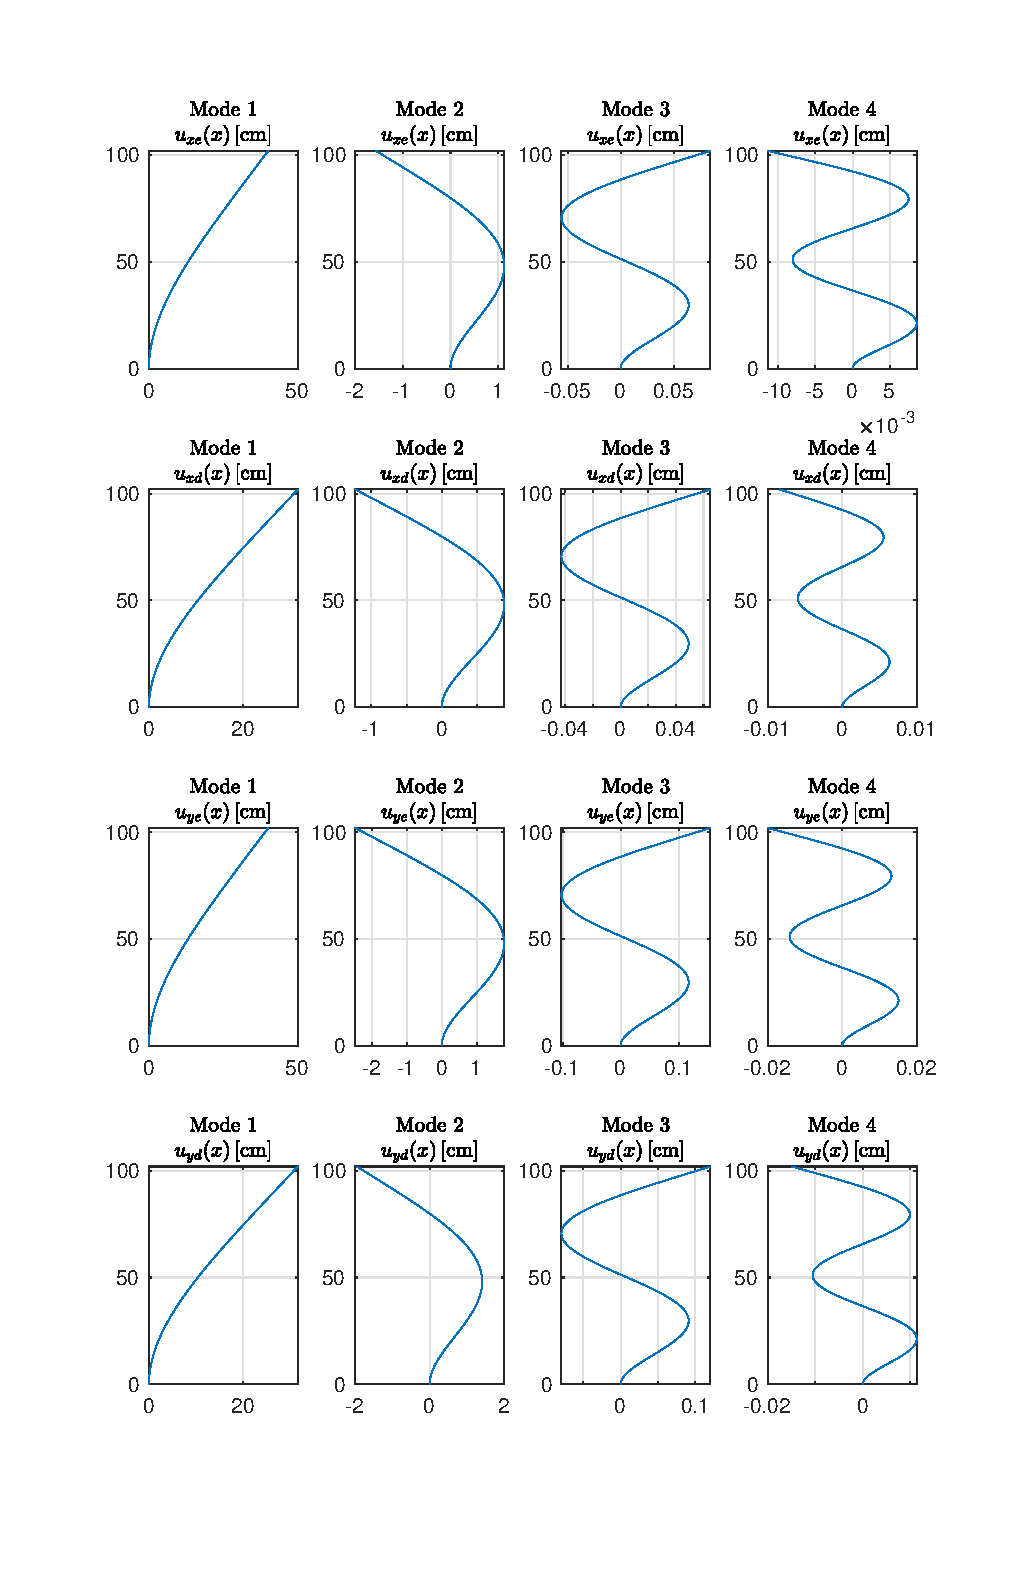
\includegraphics[width=15cm]{Modal_Displacements_HR.eps}
    \caption{Modal Displacements of the High Rise Building in Both the (X,Z) and (Y,Z) planes}
    \label{fig:I.2 Modal Displacements HR}
\end{figure}
\subsection{Total Displacements}
\paragraph{}As for the modal displacements, the total displacements of the high rise building are derived in the same way as that of the low rise building. Again, this is due to the finite number of modes of both systems, but for the high rise building only $(n=1,2,3,4)$ modes are used. Please refer to \textsc{Section}\,\ref{sec: Low Rise - Total Displacements} for the determination of these displacements. The numerical results of the total displacements at four equally dispersed heights along the high rise structure have been shown in \textsc{Table}\,\ref{tab:total elastic displacements HR} and \textsc{Table}\,\ref{tab:total design displacements HR} . The results show equal displacements produced by both the SRSS and CQC modal combination methods. Additionally, the displacements are slightly larger in the Y direction, as expected from the geometry of the building as due to moment of inertia, bending is easier in this direction, and so the displacements will be larger. Additionally, the results are identical in both for the elastic and inelastic spectrums.
\begin{table}[h]
    \centering
    \begin{tabular}{c|c|c|c|c}
    Displacement & $Height=0$ & $Height=H/3$ & $Height=2H/3$ & $Height=H$\\
    \hline
    $U_{xe}\,SRSS$ $[m]$  & $0$ & $0.0524$ & $0.1721$ & $0.3154$\\
    $U_{ye}\,SRSS$  $[m]$ & $0$ & $0.0532$ & $0.1722$ & $0.3158$\\
    $U_{xe}\,CQC$  $[m]$ & $0$ & $0.0524$ & $0.1721$ & $0.3154$\\
    $U_{ye}\,CQC$  $[m]$ & $0$ & $0.0532$ & $0.1722$ & $ 0.3158$\\
    \end{tabular}
    \caption{Total Elastic Displacements of the High Rise Building from SRSS and CQC Combinations}
    \label{tab:total elastic displacements HR}
\end{table}
\begin{table}[h]
    \centering
    \begin{tabular}{c|c|c|c|c}
    Displacement & $Height=0$ & $Height=H/3$ & $Height=2H/3$ & $Height=H$\\
    \hline
    $U_{xd}\,SRSS$ $[m]$  & $0$ & $0.0524$ & $0.1721$ & $0.3154$\\
    $U_{yd}\,SRSS$  $[m]$ & $0$ & $0.0532$ & $0.1722$ & $0.3158$\\
    $U_{xd}\,CQC$  $[m]$ & $0$ & $0.0524$ & $0.1721$ & $0.3154$\\
    $U_{yd}\,CQC$  $[m]$ & $0$ & $0.0532$ & $0.1722$ & $0.3158$\\
    \end{tabular}
    \caption{Total Elastic Displacements of the High Rise Building from SRSS and CQC Combinations}
    \label{tab:total design displacements HR}
\end{table}
\begin{figure}
    \centering
    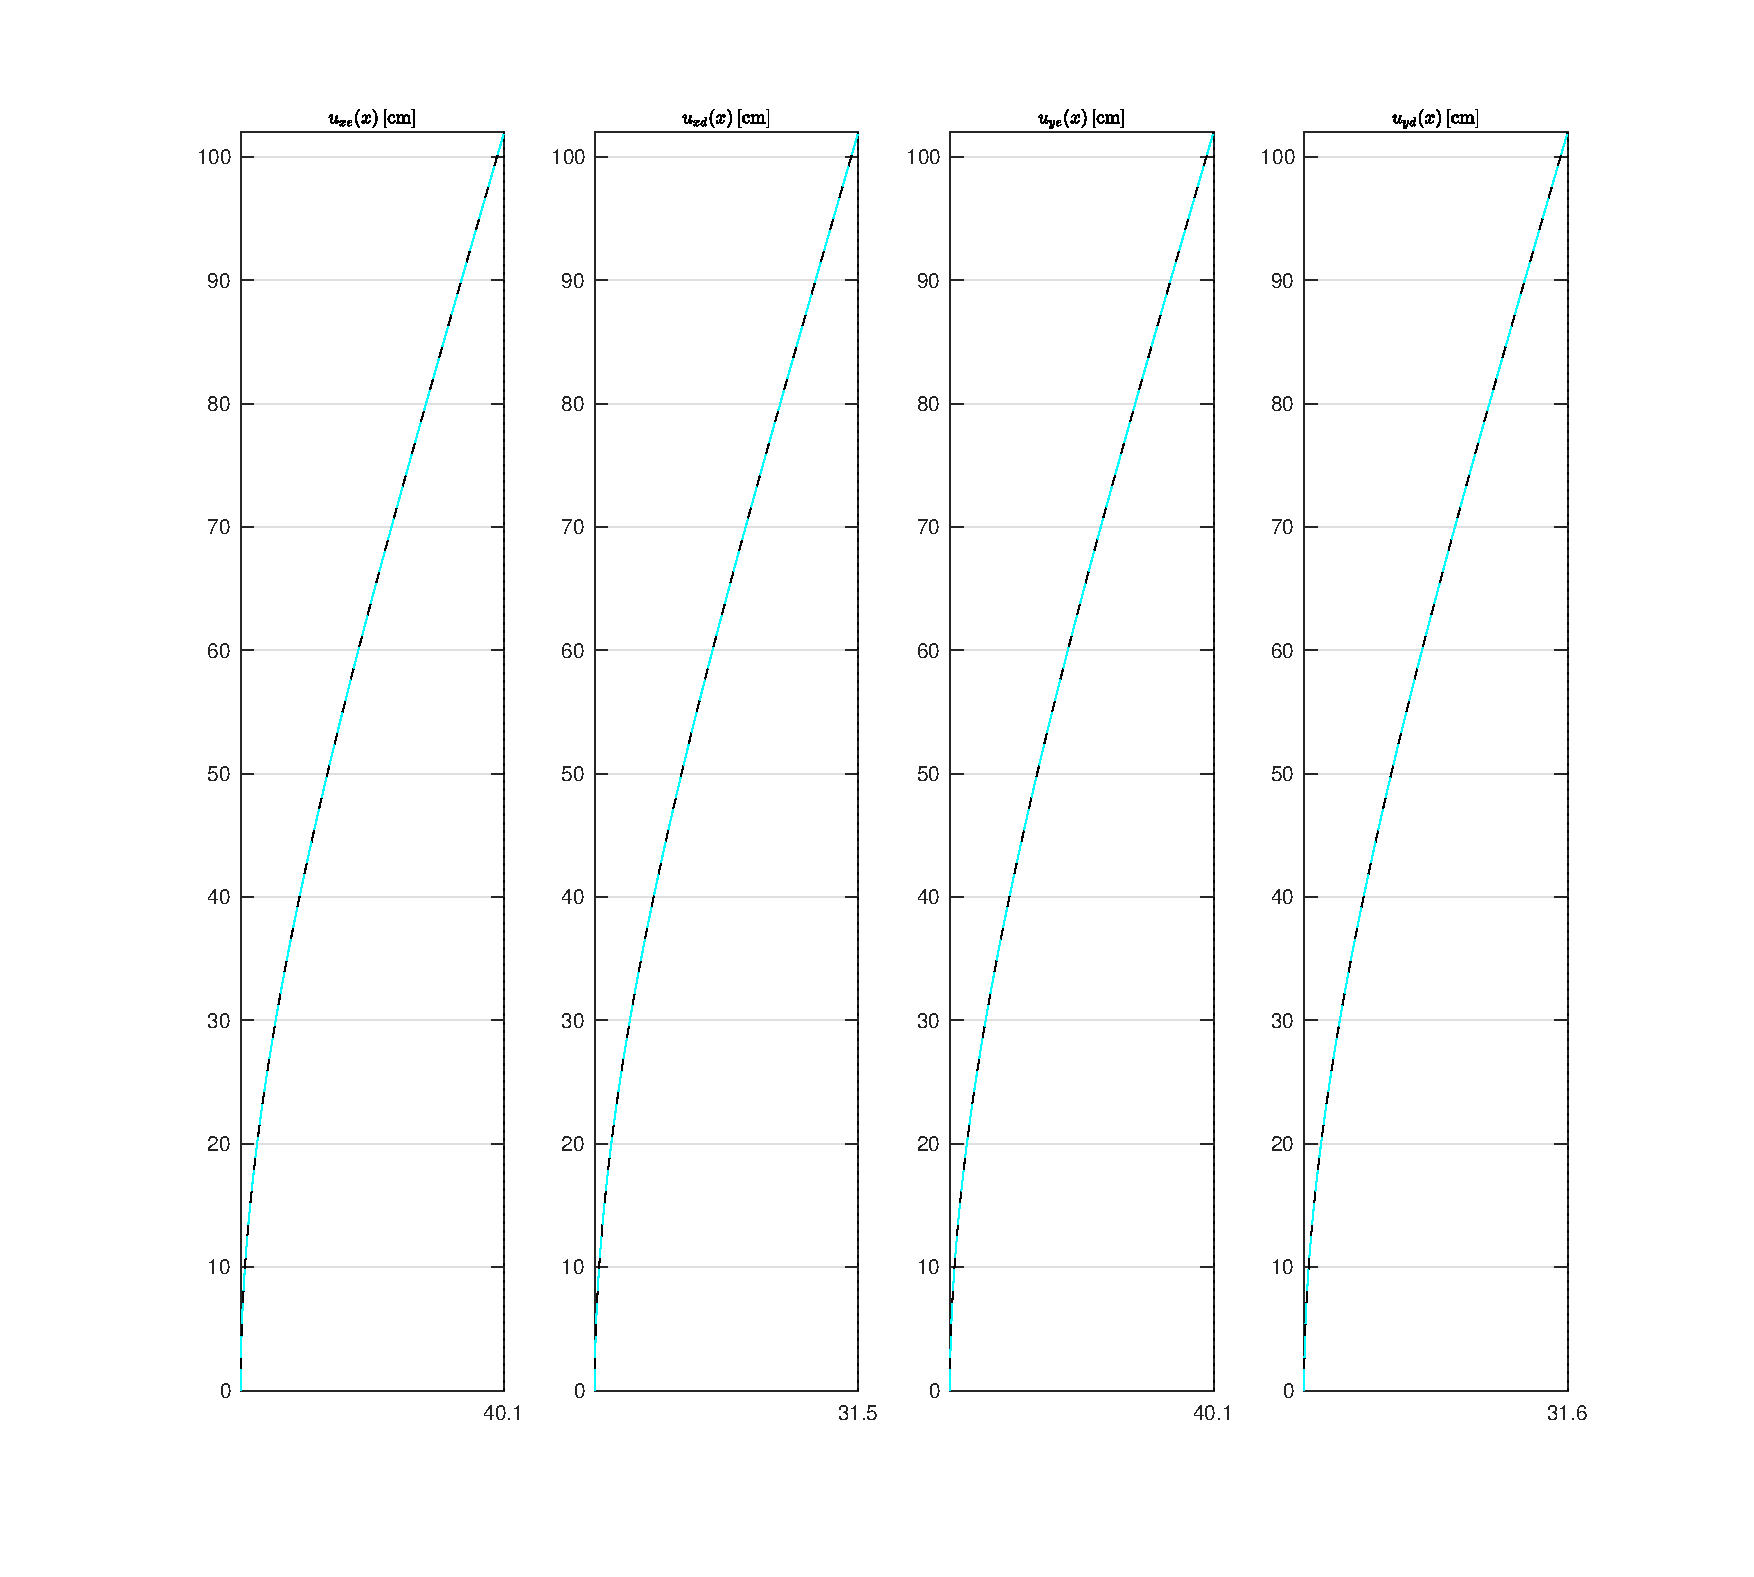
\includegraphics[width=16cm]{Total_Displacements_HR.eps}
    \caption{Total Displacements in the High Rise Building}
    \label{fig:I.2 total displacements HR}
\end{figure}
\paragraph{}\textsc{Figure}\,\ref{fig:I.2 total displacements HR} shows the total displacements in the high rise building produced by the elastic and design spectrums in both the (X,Z) and (Y,Z) planes. These results are clearly dominated by the mode shape of the first mode, as expected. Referring back to the results of the effective modal mass, and the effective mass factor of the high rise building, the first mode accounts for $61\%$ of the mass of the high rise building, which is why it is expected that its shape will physically dominate the response of high rise building. The x-axis of these results should be noted, as they look the same for both the elastic displacements and design displacements. They in fact are not and the elastic displacements show larger values in both the (X,Z) and (Y,Z) planes. 
\subsection{Modal Section Forces}
\todo{insert explanation of over design with a graph}
\paragraph{}The modal section forces of the high rise building are not the same as the low rise building and their determination will be shown in this section. These forces are only calculated for their elastic displacements. This is because the high rise building is modelled as a statistically determinant structure and does not have the ability to redistribute forces after any  yielding occurs in the structure. This means that no inelastic deformation can occur in the structure, and therefore the section forces must be determined accordingly. The determination of the modal shear forces and modal bending moments is shown in \textsc{Equation}\,\eqref{eq:I.2 - modal shear force HR} and \textsc{Equation}\,\eqref{eq:I.2 - modal shear force HR}
\begin{equation}
    F_i(x)=E_c\,I\,MPF_i\,\phi^{'''}(x)\,S_{ed,i}
    \label{eq:I.2 - modal shear force HR}
\end{equation}
\begin{equation}
    M_i(x)=E_c\,MPF_i\,\phi^{''}(x)\,S_{ed,i}
\end{equation}
\paragraph{}Where,
\begin{itemize}
\begin{small}
    \item $F_i(x)$ is the modal shear force $[N]$ 
    \item $M_i(x)$ is the modal bending moment $[Nm]$
    \item $E_c$ is the Young's Modulus of concrete given in \textsc{Table}\,\ref{tab: specifications - material properties} $[kg/m^3]$
    \item $I$ is the moment of inertia of the structure $[m^4]$
    \begin{itemize}
        \item $I_x$ is used to calculate forces in the Y direction
        \item $I_y$ is used to calculate forces in the X direction
    \end{itemize}
    \item $MPF_i$ is the modal participation factor of mode $(i=1,2,3,4)$ as determined in \textsc{Equation}\,\eqref{eq:I.1 - Modal Participation Factor - High Rise} $[-]$
    \item $\phi^{'''}(x)$ is the third derivation of the mode shape given in \textsc{Equation}\,\eqref{eqI.1:governing equation 2} $[-]$
    \item $\phi^{''}(x)$ is the second derivation of the mode shape given in \textsc{Equation}\,\eqref{eqI.1:governing equation 2} $[-]$
    \item $S_{ed,i}$ is the elastic modal displacement of mode $(i=1,2,3,4)$ $[m]$
\end{small}
\end{itemize}
\paragraph{}The physical results of the modal shear force and modal bending moment can be seen in \textsc{Figure}\,\ref{fig:I.2 - HR Shear force and bending moment X} and \textsc{Figure}\,\ref{fig:I.2 - HR Shear force and bending moment Y}.
\newpage
\begin{figure} [h]
    \centering
    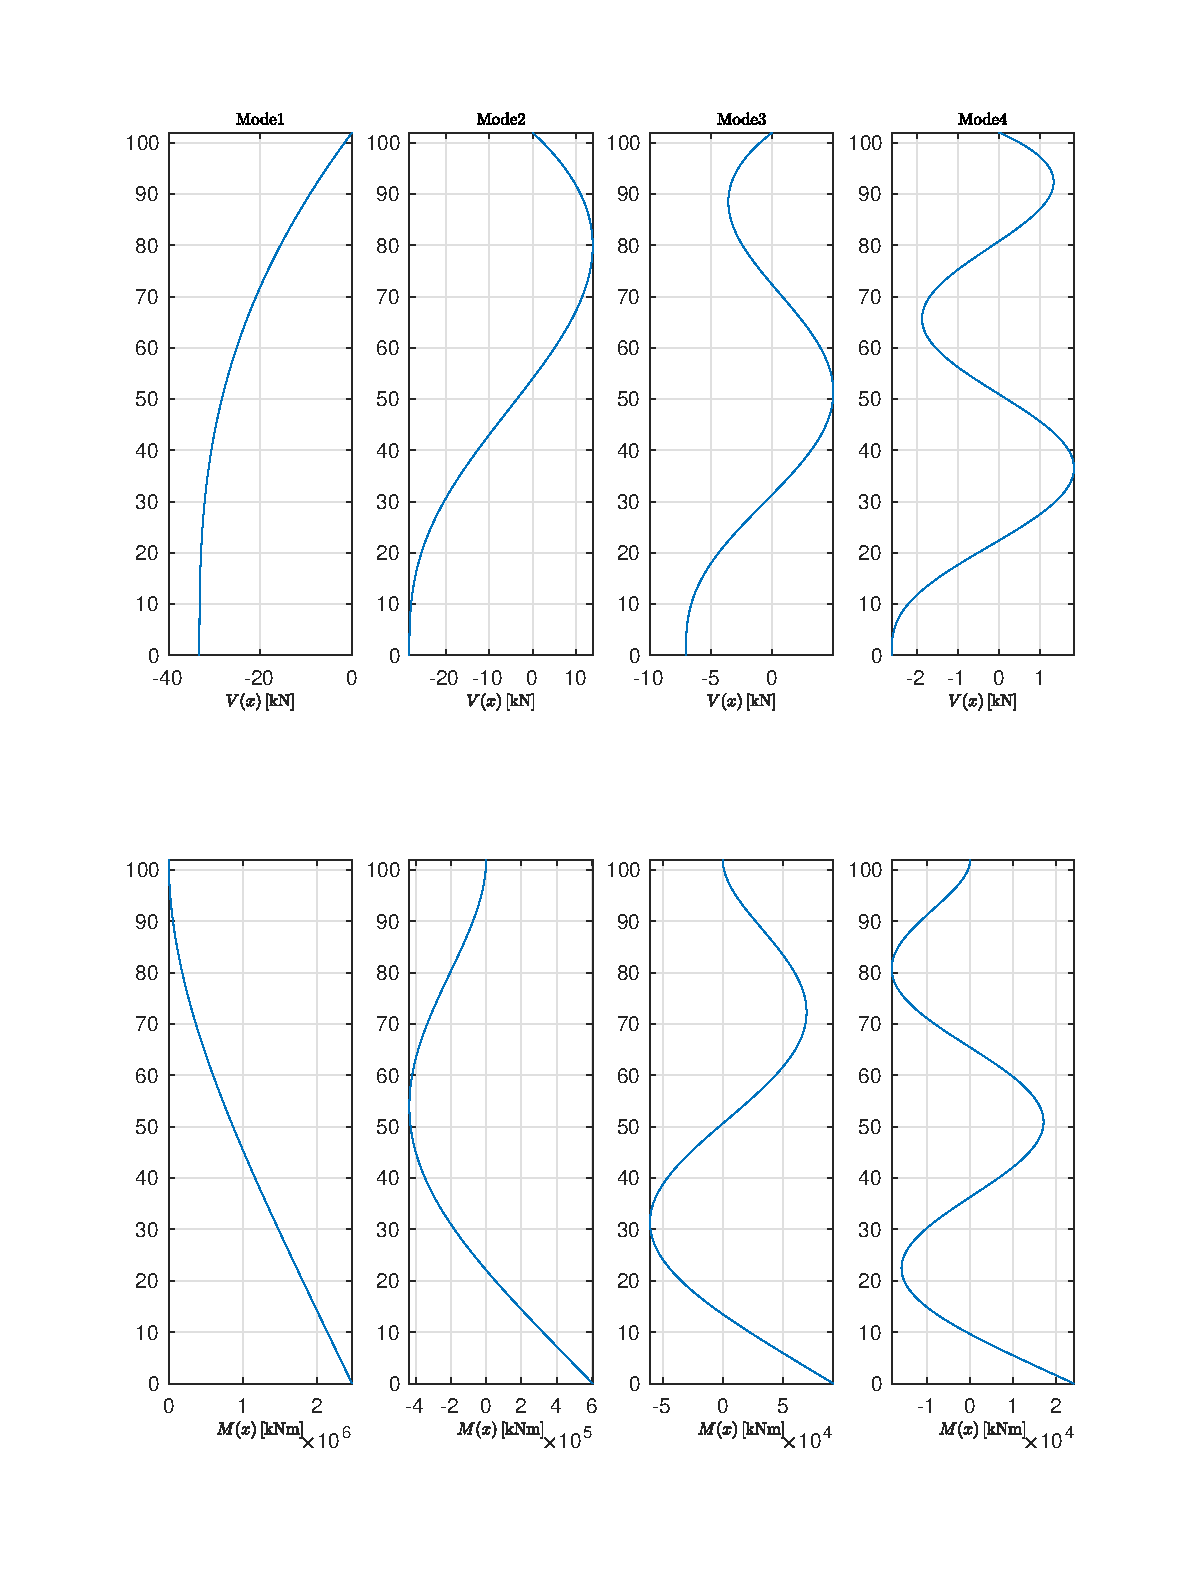
\includegraphics[width=16cm]{Modal_Section_Forces_X.eps}
    \caption{Modal Shear Force and Bending Moment in the X direction}
    \label{fig:I.2 - HR Shear force and bending moment X}
\end{figure}
\newpage
\begin{figure} [h]
    \centering
    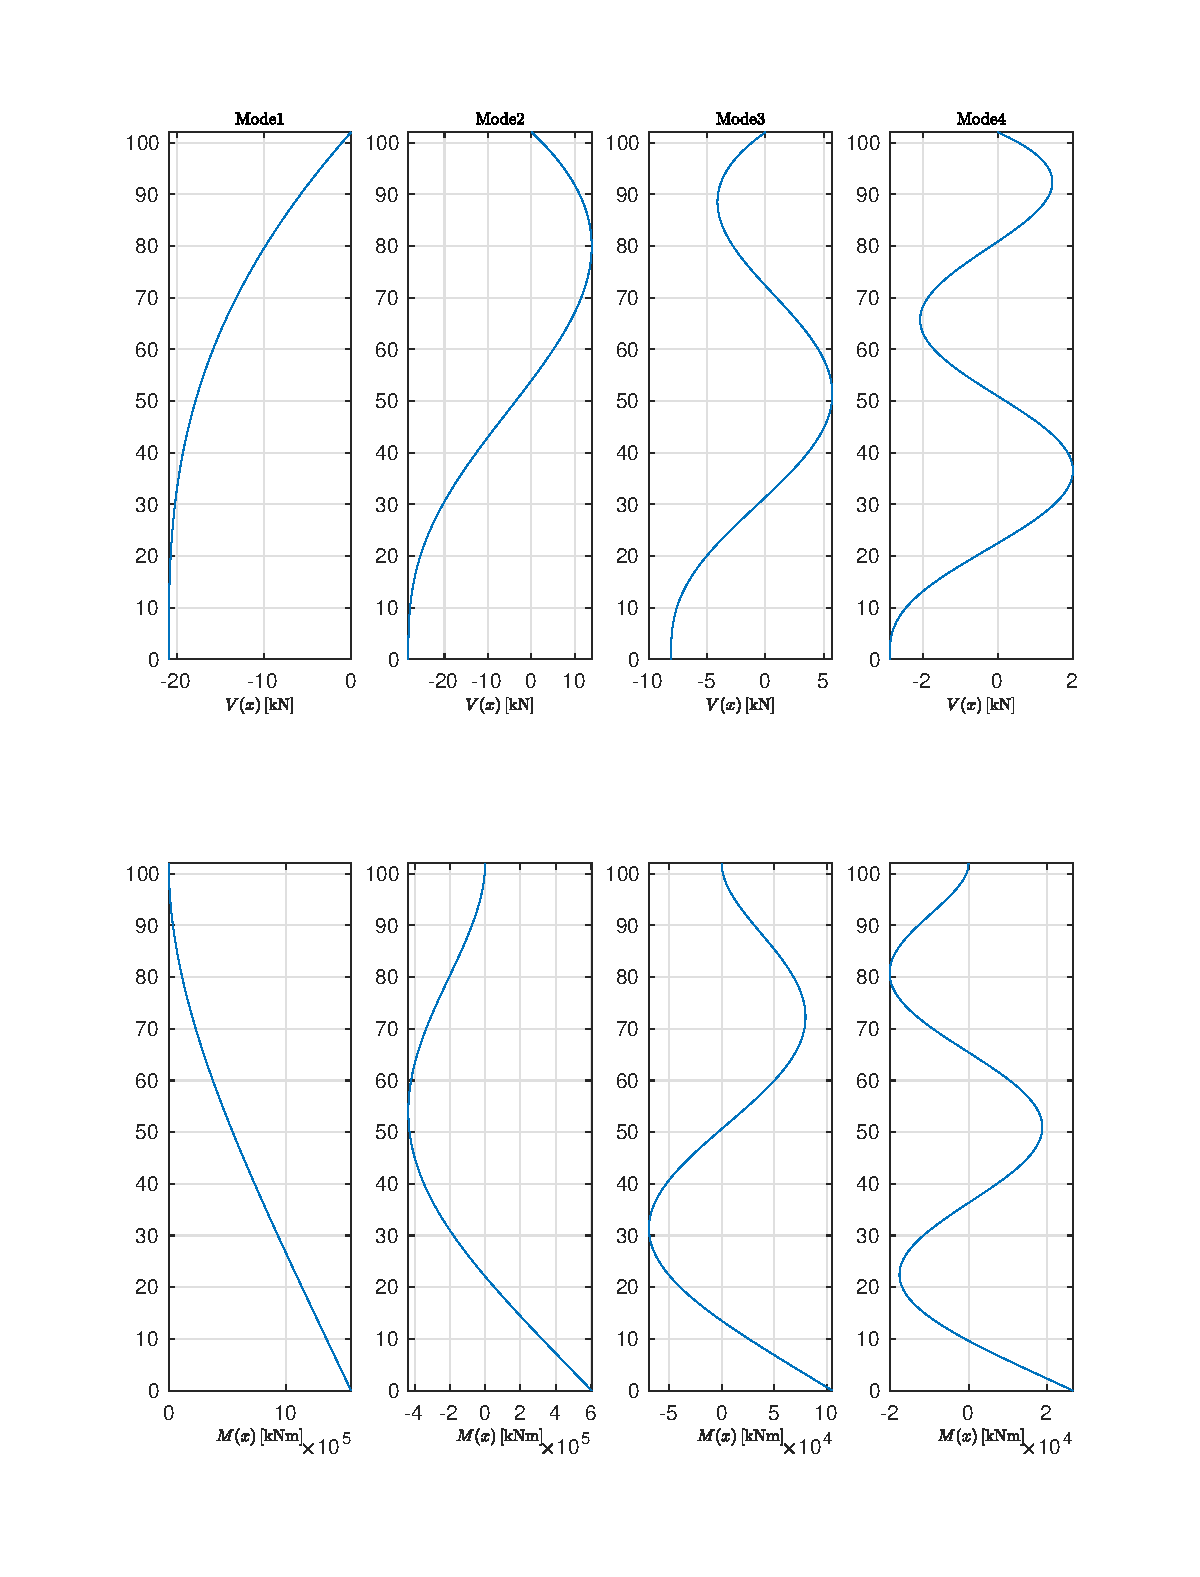
\includegraphics[width=16cm]{Modal_Section_Forces_Y.eps}
    \caption{Modal Shear Force and Bending Moment in the Y direction}
    \label{fig:I.2 - HR Shear force and bending moment Y}
\end{figure}
%\paragraph{}The numerical results of the modal shear forces and modal bending moment can be seen in \textsc{Table}\,\ref{tab:modal section forces H=0}, \textsc{Table}\,\ref{tab:modal section forces H=1/2}, \textsc{Table}\,\ref{tab:modal section forces H=3/4}, and \textsc{Table}\,\ref{tab:modal section forces H=1}. These
%\begin{table}[]
%    \centering
 %   \begin{tabular}{c|c|c|c|c}
  %  $Mode$ & $1$ & $2$ & $3$ & $4$ \\
   % \hline
    %$F_x$ $[N]$  & $$ & $$ & $$ & $$ \\
%    $F_y$  $[N]$ & $$ & $$ & $$ & $$\\
 %   $M_x$ $[Nm]$ & $$ & $$ & $$ & $$\\
  %  $M_y$ $[Nm]$ & $$ & $$ & $$ & $$\\
   % \end{tabular}
    %\caption{Modal Shear Forces and Bending Moments at Height of Building = 0}
%    \label{tab:modal section forces H=0}
%\end{table}
%\begin{table}[]
 %   \centering
  %  \begin{tabular}{c|c|c|c|c}
   % $Mode$ & $1$ & $2$ & $3$ & $4$ \\
    % \hline
%    $F_x$ $[N]$  & $$ & $$ & $$ & $$\\
 %   $F_y$ $[N]$  & $$ & $$ & $$ & $$\\
  %  $M_x$ $[Nm]$  & $$ & $$ & $$ & $$\\
   % $M_y$ $[Nm]$  &  & $$ & $$ & $$ & $$\\
  %  \end{tabular}
   % \caption{Modal Shear Forces and Bending Moments at Height of Building = H/2}
    %\label{tab:modal section forces H=1/2}
%\end{table}
%\begin{table}[]
 %   \centering
  %  \begin{tabular}{c|c|c|c|c}
   % $Mode$ & $1$ & $2$ & $3$ & $4$ \\
    % \hline
    %$F_x$ $[N]$ & $$ & $$ & $$ & $$\\
%    $F_y$  $[N]$ & $$ & $$ & $$ & $$\\
 %   $M_x$ $[Nm]$  & $$ & $$ & $$ & $$\\
  %  $M_y$  $[Nm]$ & $$ & $$ & $$ & $$\\
   % \end{tabular}
    %\caption{Modal Shear Forces and Bending Moments at Height of Building = 3H/4}
    %\label{tab:modal section forces H=3/4}
%\end{table}
%\begin{table}[]
 %   \centering
  %  \begin{tabular}{c|c|c|c|c}
   % $Mode$ & $1$ & $2$ & $3$ & $4$ \\
    % \hline
%    $F_x$ $[N]$  & $$ & $$ & $$ & $$\\
 %   $F_y$  $[N]$ & $$ & $$ & $$ & $$\\
  %  $M_x$ $[Nm]$ & $$ & $$ & $$ & $$\\
   % $M_y$  $[Nm]$ & $$ & $$ & $$ & $$\\
    %\end{tabular}
%    \caption{Modal Shear Forces and Bending Moments at Height of Building = H}
 %   \label{tab:modal section forces H=1}
%\end{table}
\subsection{Total Section Forces} 
\paragraph{}As per the modal section forces, the total section forces of the high rise building are the same as that of the low rise building using the SRSS and CQC methods. The determination of these can be found in \textsc{Section}\,\ref{sec: Low Rise - Total Section Forces}. The results have been displayed on plots that show the relationship between the height of the building and the section force for both the X and Y directions in \textsc{Figure}\,\ref{fig:I.2 total section forces HR}. It should be noted that the graphical display of these results has not been normalized and so attention should be drawn to the values on the x-axis as these plots should not be directly compared between shear forces and bending moments. The numerical results which have been shown at four equal height intervals within the building can be seen in \textsc{Table}\,\ref{tab:total section forces HR SRSS}, and \textsc{Table}\,\ref{tab:total section forces HR CQC}. These results show that one modal combination method did not consistently produce larger or smaller values, as expected. Instead the SRSS and CQC methods produced values that are sometimes larger and sometimes smaller for certain forces at certain heights. Typically, the CQC method produces larger values than that of the SRSS. Although, the discrepancies are within a small enough range that this concern is of minimal significance.
\begin{table}[h]
    \centering
    \begin{tabular}{c|c|c|c|c}
    Force & $Height=0$ & $Height=H/3$ & $Height=2H/3$ & $Height=H$\\
    \hline
    $F_x$ $[N]$  & $44.3621$ & $36.3079$ & $24.3849$ & $0.0013$\\
    $F_y$  $[N]$ & $36.2672$ & $26.6998$ & $17.4815$ & $0.0014$\\
    $M_x$ $[Nm]$  & $2,542.6$ & $1,377.9$ & $548.4725$ & $4.4008$x$10^{-11}$\\
    $M_y$  $[Nm]$ & $1,670.0$ & $891.0171$ & $447.5424$ & $4.8577$x$10^{-11}$\\
    \end{tabular}
    \caption{Total Section Forces of the High Rise Building from SRSS Combination}
    \label{tab:total section forces HR SRSS}
\end{table}
\begin{table}[h]
    \centering
    \begin{tabular}{c|c|c|c|c}
    Force & $Height=0$ & $Height=H/3$ & $Height=2H/3$ & $Height=H$\\
    \hline
    $F_x$ $[MN]$  & $44.3667$ & $36.3090$ & $24.3841$ & $0.0013$\\
    $F_y$  $[MN]$ & $36.2725$ & $26.7006$ & $17.4808$ & $0.0014$\\
    $M_x$ $[MNm]$  & $2,542.7$ & $1377.9$ & $548.4301$ & $4.4008$x$10^{-11}$\\
    $M_y$  $[MNm]$ & $1,670.0$ & $891.0033$ & $447.4976$ & $4.8577$x$10^{-11}$\\
    \end{tabular}
    \caption{Total Section Forces of the High Rise Building from CQC Combination}
    \label{tab:total section forces HR CQC}
\end{table}
\newpage
\begin{figure}[h]
    \centering
    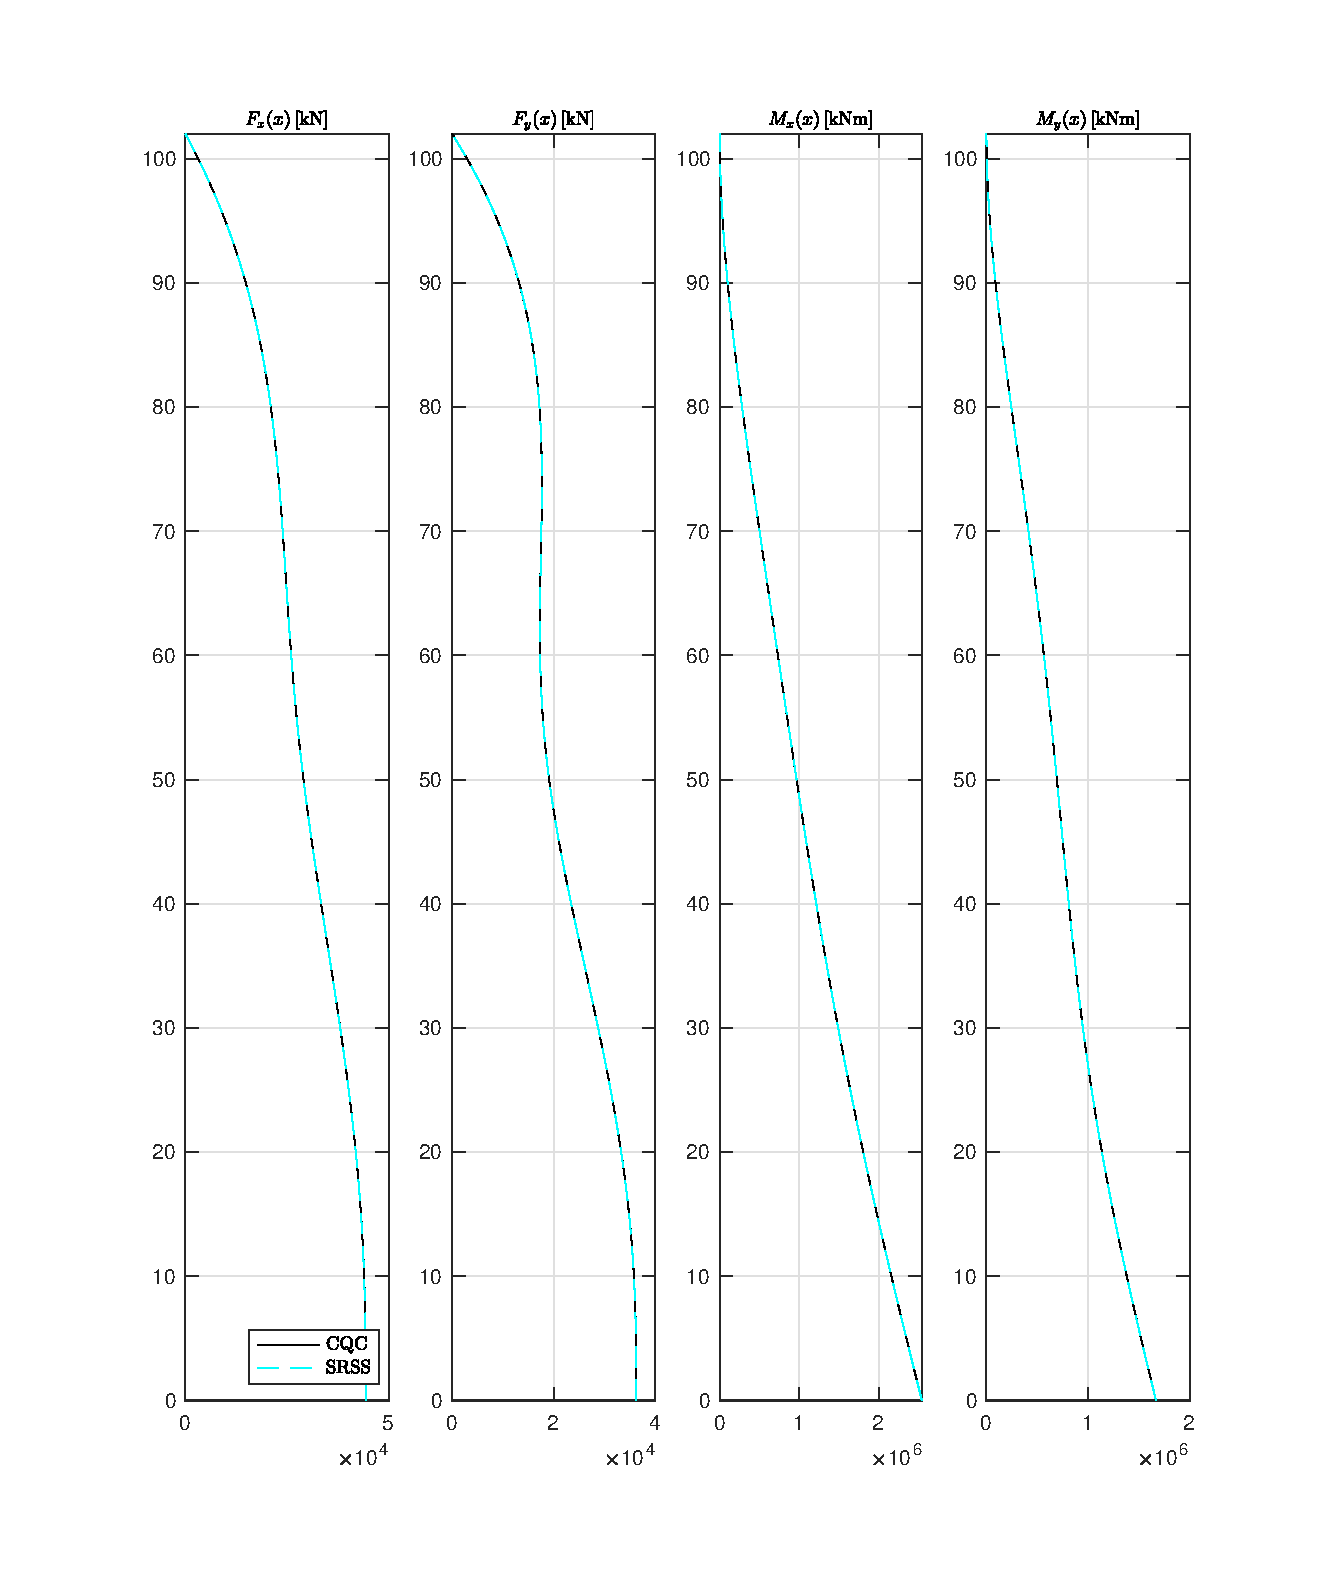
\includegraphics[width=14cm]{Total_Section_Forces_HR.eps}
    \caption{Total Section Forces of the High Rise Building in both X and Y directions}
    \label{fig:I.2 total section forces HR}
\end{figure}



\chapter{Structural Response - Time History Analysis}
\paragraph{}The time history analysis of the low rise and high rise structures is determined using the Duhamel integration approach. For the purpose of this analysis, it is assumed that both the high rise and low rise buildings are linear systems. The time history analysis of the structures uses the seismic motions recorded from Coalinga. 

\paragraph{}The time history analysis for the low rise building was performed using Duhamel integration for both the (X,Z) plane and (Y,Z) plane of the structure. To obtain this the modes must be assessed independently, and so, the MDOF system's accelerogram is transformed into an equivalent accelerogram for a SDOF system. 

\section{Acceleration Scaling}
\paragraph{}Before conducting the time history analysis of the structures, the provided data must be scaled to provide accurate results that are comparable to the modal response analysis. The data for Coalinga ground acceleration has a different peak acceleration than that of the peak ground acceleration provided in \textsc{Table}\,\ref{tab: specifications - seismic}. The acceleration must be scaled, so that the peak ground acceleration is equal for both the modal response and time history analyses. Once this is the case, the structural response can be accurately compared. The scaling of this acceleration is done using \textsc{Equation}\,\eqref{eq:I.3 - Accelerogram Scaling} below. The acceleration scaling is independent of the structural elements and therefore is the same for both the low rise building (in both (X,Z) and (Y,Z) directions) and the high rise building. 
\begin{equation}
    a_g = a\,\dfrac{PGA_1}{PGA_2}
   \label{eq:I.3 - Accelerogram Scaling}
\end{equation}
\paragraph{}Where,
\begin{itemize}
\begin{small}
    \item $a_g$ is the scaled ground acceleration used for the time history analysis $[m/s^2]$
    \item $a$ is the acceleration data provided from the Coalinga data $[m/s^2]$
    \item $PGA_1$ is the provided peak ground acceleration provided as given in \textsc{Table}\,\ref{tab: specifications - seismic} $[m/s^2]$
    \item $PGA_2$ is the peak ground acceleration from the Coalinga  data set $[m/s^2]$
\end{small}
\end{itemize}
\paragraph{}The results of the acceleration scaling have been provided in \textsc{Figure}\,\ref{fig:acceleration scalling}. This figure shows that the scaled acceleration has a smaller range and peak values than the acceleration of the Coalinga data set, as expected. 
\begin{figure}
    \centering
    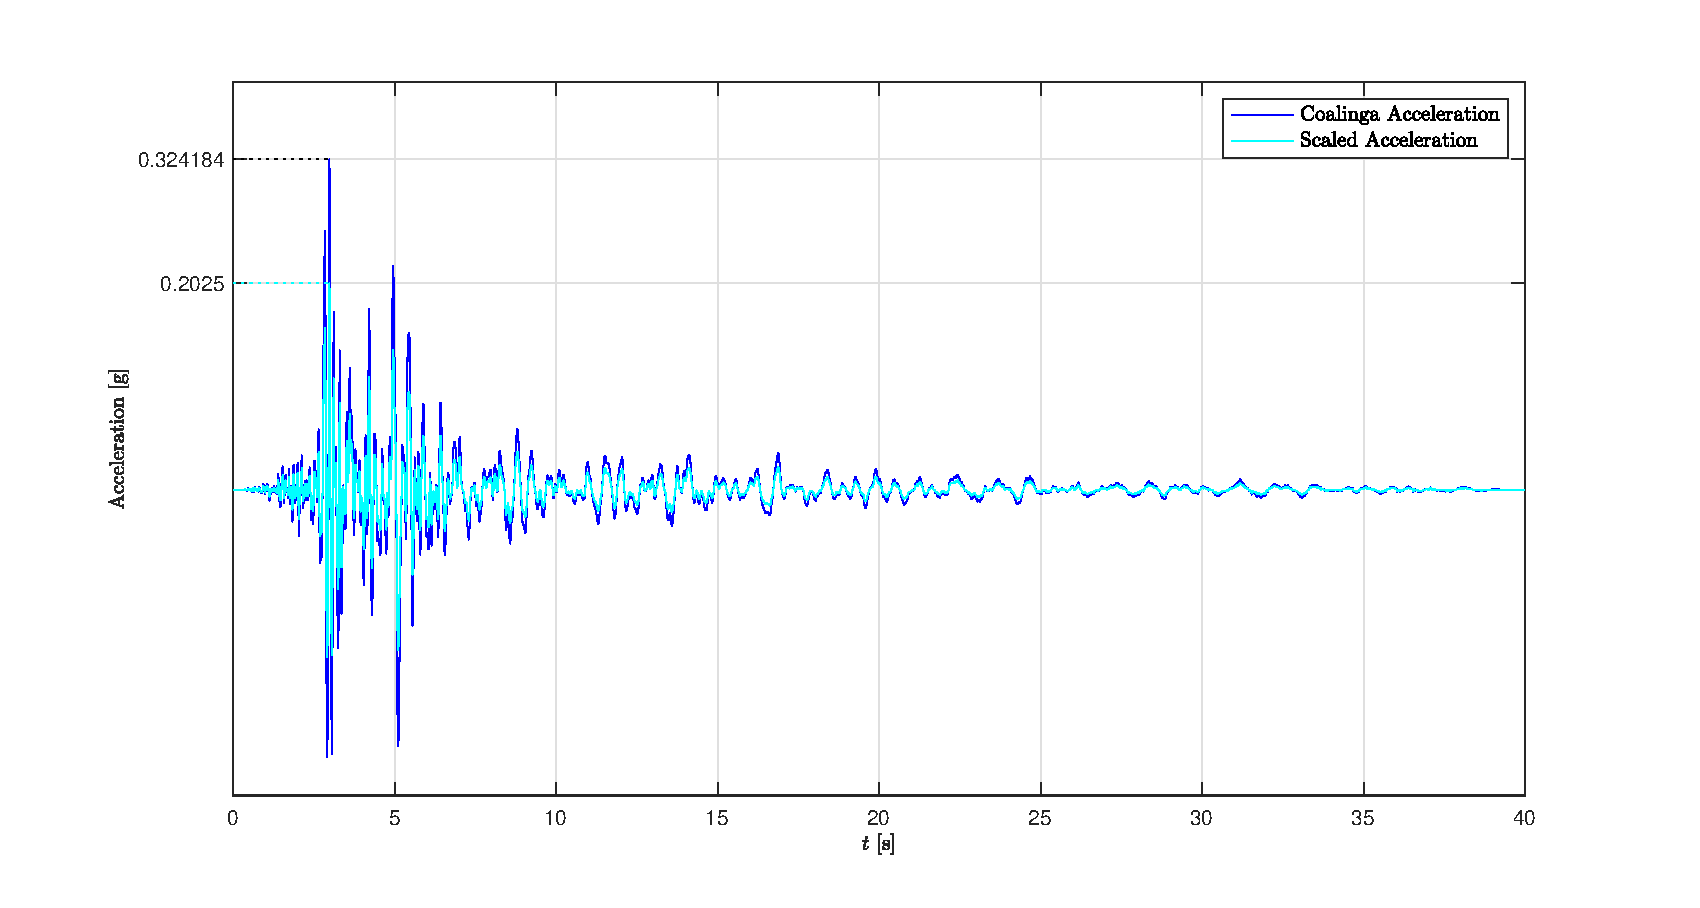
\includegraphics[width=16cm]{scaled_acceleration.eps}
    \caption{Comparison of the original acceleration and the scaled acceleration}
    \label{fig:acceleration scalling}
\end{figure}
\section{Time Scaling}
\paragraph{}In addition to the acceleration data, time must also be scaled appropriately. To ensure accuracy, the $dt$ used in the analysis has to be smaller or equal to the value produced using \textsc{Equation}\,\eqref{eq:I.3 time scaling}. For a single degree of freedom system the minimum period is used. For a multi degree of freedom system, such as both the low rise and the high rise buildings there is more work required. These systems must use the same period for all degrees of freedom, therefore the dt has to be smaller than or equal to the value obtained from \textsc{Equation}\,\eqref{eq:I.3 time scaling} below using the minimum period of all the degrees of freedom. For the low rise building this must be assesed in both the (X,Z) and (Y,Z) planes as it is not independent of the behavior of the structure.
\begin{equation}
    dt = \dfrac{1}{20}\,T
    \label{eq:I.3 time scaling}
\end{equation}
\paragraph{}Where,
\begin{itemize}
\begin{small}
    \item $dt$ is the time step $[s]$
    \item $T$ is the period $[s]$
\end{small}
\end{itemize}
\paragraph{}The accelerogram data provided does not include data with a small enough time step to meet the requirements of the multi degree of freedom structures being analyzed. A spline interpolation of the function is to be performed to estimate the required time step for the building.
\section{Damped Angular Natural Frequency}
\paragraph{}Prior to beginning the time history analysis of the Low Rise building, the frequency of the system must be adjusted to account for the effect of the damping of the system on the frequency of the modes. 
\begin{equation}
    \omega_d=\omega_n\,\sqrt{1-\xi^2}
    \label{eq:I.3 - damped natural angular frequency}
\end{equation}
\paragraph{}Where,
\begin{itemize}
\begin{small}
    \item $\omega_d$ is the damped natural angular frequency $[rad/s]$
    \item $\omega_n$ natural angular frequency of mode $(n=1,2,...,12)$ $[rad/s]$
    \item $\xi$ is the damping given in \textsc{Table}\,\ref{tab: Specifications - Design LowRB } expressed as a ratio not a percent $[-]$
\end{small}
\end{itemize}
\section{Dumahel Integral}
\paragraph{}The time history analysis is used to determine the modal displacement at a degree of freedom with respect to time along which the ground is accelerating. This analysis is determined using the governing equation shown in \textsc{Equation}\,\eqref{eq:I.3 - governing equation for time history analysis}, and is assessed using the Duhamel integral. The principles from Simpson's rule are then later applied to these equations for integration \cite{Tobias}. 
\begin{equation}
    x(t)=sin\,\omega_n\,t\dfrac{1}{\bar{m}\omega_n}\int^t_0\,p(t)\,cos\,\omega_n\,\tau\,d\tau\,-\,cos\,\omega_n\,t\dfrac{1}{\bar{m}\omega_n}\int^t_0\,p(t)\,sin\,\omega_n\,\tau\,d\tau\,
    \label{eq:I.3 - governing equation for time history analysis}
\end{equation}
\paragraph{}Where,
\begin{itemize}
\begin{small}
    \item $x(t)$ is the function of the displacement from degree of freedom $(N=1,2,...,12)$ over time, $t$ $(N=1,2,...,12)$ $[m(s)]$
    \item $\omega_d$ is the damped natural angular frequency as given in \textsc{Equation}\,\eqref{eq:I.3 - damped natural angular frequency} $[rad/s]$
    \item $t$ is the time $[s]$
    \item $\bar{m}$ is the mass per unit length of the structure $[kg/m]$
    \item $p(t)$ is the relationship of the unit impulse response of the system
    \item $\tau$ is a length of time over which the structure is subjected to strong ground motions $[s]$
    \item $d\tau$ is an infintesimally small length of time over which the structure is subjected to strong ground motions $[s]$
\end{small}
\end{itemize}
\paragraph{}This equation is assessed using using the duhamel integral and the relationship can be simplified as shown below in \textsc{Equation}\,\eqref{eq:I.3 - simplified governing equation} \cite{Tobias}.
\begin{equation}
    x(t)=A(t)sin\omega_d\,t-B(t)sin\omega_d\,t
    \label{eq:I.3 - simplified governing equation}
\end{equation}
\paragraph{}Where,
\begin{itemize}
\begin{small}
    \item $x(t)$ is the function of the displacement from a movement of degree of freedom $(n=1,2,...,12)$ over time, $[m(s)]$
     \item $\omega_d$ is the damped natural angular frequency as given in \textsc{Equation}\,\eqref{eq:I.3 - damped natural angular frequency} $[rad/s]$
    \item $t$ is the time $[s]$
    \item $A(t)$ is a constant function describing the unit impulse to be described below in \textsc{Equation}\,\eqref{eq:I.3 - constant function A(t)} 
    \item $B(t)$ is a constant function describing the unit impulse to be described below in \textsc{Equation}\,\eqref{eq:I.3 - constant function B(t)}
\end{small}
\end{itemize}
\paragraph{}The constant functions describing the unit impulse are give below in \textsc{Equation}\,\eqref{eq:I.3 - constant function A(t)} and \textsc{Equation}\,\eqref{eq:I.3 - constant function B(t)} \cite{Tobias}.
\begin{equation}
    A(t)=\dfrac{1}{\bar{m}\omega_d}\,\int^t_0\,f(\tau)\dfrac{e^{-\xi\,\omega_n\,\tau}}{e^{-\omega_n\,t}}\,cos\left(\omega_d\,t\right)d\tau
    \label{eq:I.3 - constant function A(t)}
\end{equation}
\begin{equation}
    B(t)=\dfrac{1}{\bar{m}\omega_d}\,\int^t_0\,f(\tau)\dfrac{e^{-\xi\,\omega_n\,\tau}}{e^{-\omega_n\,t}}\,sin\left(\omega_d\,t\right)d\tau
    \label{eq:I.3 - constant function B(t)}
\end{equation}
\paragraph{}Where, 
\begin{itemize}
\begin{small}
    \item $A(t)$ is a constant function of the unit impulse
    \item $B(t)$ is a constant function of the unit impulse
    \item $\bar{m}$ is the mass per unit length $[kg/m]$
    \item $\omega_d$  is the damped natural angular frequency given in \textsc{Equation}\,\eqref{eq:I.3 - damped natural angular frequency} $[rad/s]$
    \item $f(\tau)$ ...?
    \item $\xi$ is the damping ratio given in \textsc{Table}\,\ref{tab: Specifications - Design LowRB } $[\%]$
    \item $\omega_n$ is the natural frequency of a mode $[rad/s]$ $(n=1,2,...,12)$
    \item $\tau$ $[s]$
    \item $t$ is the time $[s]$
\end{small}
\end{itemize}
\paragraph{} Functions $M_1$ and $M_2$ describe the decay of the damping of the system. The function $F$ accounts for the effect of the damping natural angular frequency over a finite increment of time. These functions are dependent on the modal response of the system, and are independent of the time variable. They are used as constants for the overall derivation of the time history analysis of the structure \cite{Tobias}.
\begin{equation}
    M_1 = 4\,e^{-\xi\,\omega_n\,dt}
    \label{eq:I.3 - Damping Decay M1}
\end{equation}
\begin{equation}
    M_2 = e^{-2\,\xi\,\omega_n\,dt}
     \label{eq:I.3 - Damping Decay M2}
\end{equation}
\paragraph{}Where,
\begin{itemize}
\begin{small}
    \item $M_1$ is a constant function used to describe the exponential decay of the damping of the system $[-]$
    \item $M_2$ is a constant function used to describe the exponential decay of the damping of the system $[-]$
    \item $\xi$ is the damping ratio as given in \textsc{Table}\,\ref{tab: Specifications - Design LowRB } $[m]$
     \item $\omega_n$ is the natural frequency of a mode $(n=1,2,...,12)$ $[rad/s]$
    \item $dt$ is an finite increment of time $t$ $[s]$
\end{small}
\end{itemize}
\begin{equation}
    F=\dfrac{dt}{3\,\omega_d}
\end{equation}
\todo{Why is there no m in this equation????}
\paragraph{}Where,
\begin{itemize}
\begin{small}
    \item $F$ is a constant function used to describe the effect of the damping natural angular frequency over a finte increment of time.
    \item $dt$ is an finite increment of time $t$
    \item $\omega_d$ is the damped natural angular frequency given in \textsc{Equation}\,\eqref{eq:I.3 - damped natural angular frequency}
\end{small}
\end{itemize}
\paragraph{}The next part of the analysis begins to use a time step, $N$, to simplify the integration process of the over arching relationship described in \textsc{Equation}\,\eqref{eq:I.3 - governing equation for time history analysis}. The use of the time step reduces the data quantity as it does not use $(N=1,2,3,4,5,6,...)$ but rather $(N=2,4,6,...)$. It is important to note as its simplification sacrifices the accuracy of the analysis as it only uses every other value.  $y_N$ and $z_N$ are functions dependent on the time step $(N=2,4,6,...)$ that describe the relationship between the scaled ground acceleration, damped natural angular frequency, and the time at the specific time step \cite{Tobias}.
\begin{equation}
        y_N=a_N\,cos\,\left(\omega_d\,t_N\right)
        \label{eq:I.3 - yN}
\end{equation}
\begin{equation}
        z_N=a_N\,sin\,\left(\omega_d\,t_N\right)
        \label{eq:I.3 - zN}
\end{equation}
\paragraph{}Where,
\begin{itemize}
\begin{small}
    \item $y_N$ is the constant function used for the derivation of $A(t)$ $[-]$
    \item $z_N$ is is the constant function used for the derivation of $B(t)$ $[-]$
    \item $a_N$ the scaled ground acceleration determined in \textsc{Equation}\,\eqref{eq:I.3 - Accelerogram Scaling} at time $t_N$ $[m/s]$
    \item $\omega_{d}$ is the damped natural angular frequency of the system for a specific mode $(i=1,2,...,12)$ as defined in \textsc{Equation}\,\eqref{eq:I.3 - damped natural angular frequency} $[rad/s]$
    \item $t_N$ is the time at time step $(N=2,4,6,...)$ $[s]$
\end{small}
\end{itemize}
\paragraph{}Using these constants described above and applying them to the constant functions $A(t)$ and $B(t)$, the resulting functions given in \textsc{Equation}\,\eqref{eq:I.3 - AN} and \textsc{Equation}\,\eqref{eq:I.3 - BN} are produced as shown below \cite{Tobias}.
\begin{equation}
    A_N=A_{N-2}\,M_2+a\,\left(y_{N-2}\,M_2+y_{N-1}M_1+y_N\right)
    \label{eq:I.3 - AN}
\end{equation}
\begin{equation}
    B_N=B_{N-2}\,M_2+a\,\left(z_{N-2}\,M_2+z_{N-1}M_1+z_N\right)
    \label{eq:I.3 - BN}
\end{equation}
\paragraph{}Where,
\begin{itemize}
\begin{small}
    \item $A_N$ is the numerical result of the $A(t)$ function at a time $t_N$ where $(N=2,4,6,...)$ $[-]$
    \item $B_N$ is the numerical result of the $B(t)$ function at a time $t_N$ where $(N=2,4,6,...)$ $[-]$
    \item $M_2$ is the constant function describing the decay of the damping of the system as given in \textsc{Equation}\,\eqref{eq:I.3 - Damping Decay M2} $[-]$
    \item $M_1$ is the constant function describing the decay of the damping of the system as given in \textsc{Equation}\,\eqref{eq:I.3 - Damping Decay M2} $[-]$
    \item $y_N$ is the numerical result of the $y_N$ function given in \textsc{Equation}\,\eqref{eq:I.3 - yN} $[-]$
    \item $y_{N-1}$ is the numerical result of the $y_N$ function given in \textsc{Equation}\,\eqref{eq:I.3 - yN} for a $y_N$ value that uses an $N$ value that is equal to $N-1$ of the current $N$ value being used $[-]$
    \item $y_{N-2}$ is the numerical result of the $y_N$ function given in \textsc{Equation}\,\eqref{eq:I.3 - yN} for a $y_N$ value that uses an $N$ value that is equal to $N-2$ of the current $N$ value being used $[-]$
    \item $z_N$ is the numerical result of the $y_N$ function given in \textsc{Equation}\,\eqref{eq:I.3 - zN} $[-]$
    \item $z_{N-1}$ is the numerical result of the $z_N$ function given in \textsc{Equation}\,\eqref{eq:I.3 - zN} for a $z_N$ value that uses an $N$ value that is equal to $N-1$ of the current $N$ value being used $[-]$
    \item $z_{N-2}$ is the numerical result of the $z_N$ function given in \textsc{Equation}\,\eqref{eq:I.3 - zN} for a $z_N$ value that uses an $N$ value that is equal to $N-2$ of the current $N$ value being used $[-]$
\end{small}
\end{itemize}
\paragraph{}Using the methods described above, the response of the system in the form of displacement is now determinable. This is done using \textsc{Equation}\,\eqref{eq:I.3 - response of damped system} below \cite{Tobias}. 
\begin{equation}
    x_N=A_N\,sin\left(\omega_d\,t_N\right)+B_N\,cos\left(\omega_d\,t_N\right)
    \label{eq:I.3 - response of damped system}
\end{equation}
\paragraph{}Where,
\begin{itemize}
\begin{small}
    \item $x_N$ is the numerical result that gives a value for the displacement of the system at a corresponding time $t_N$ $[m]$
    \item $A_N$ is the numerical result of the $A(t)$ function at a time $t_N$ where $(N=2,4,6,...)$ $[-]$
    \item $B_N$ is the numerical result of the $B(t)$ function at a time $t_N$ where $(N=2,4,6,...)$ $[-]$
    \item $\omega_d$ is the damped natural angular frequency of the system as described in \textsc{Equation}\,\eqref{eq:I.3 - damped natural angular frequency} $[rad/s]$
    \item $t_N$ is the time at time step $(N=2,4,6,...)$  $[s]$
\end{small}
\end{itemize}
\paragraph{}The relationship produced from \textsc{Equation}\,\eqref{eq:I.3 - response of damped system} does not give the structural response from the time history analysis. Additional steps arerequired to obtain an accurate result of the response from the structure. The result obtained from \textsc{Equation}\,\eqref{eq:I.3 - response of damped system} does not take into consideration the modal participation factor or the shapes of the modes. The functions described below provide the further derivations to account for the behavior of the modes to attain the desired structural response of the system. The modal coordinates must first be determined, as show below in \textsc{Equation}\,\eqref{eq:I.3 - modal coordinates} \cite{Tobias}.
\begin{equation}
    q_N=MPF_i\,x_N
    \label{eq:I.3 - modal coordinates}
\end{equation}
\paragraph{}Where,
\begin{itemize}
\begin{small}
    \item $q_N$ is the modal coordinates for a displacement at time $t_N$ for a mode $(i=1,2,...,12)$ $[m]$
    \item $MPF_i$ is the modal participation factor of the mode $(i=1,2,...,12)$ as described in \textsc{Equation}\,\eqref{eq:I.1 - Modal Participation Factor - Low Rise} $[-]$
    \item $x_N$ is the displacement of the mode $(i=1,2,...,12)$ at a time $t_N$ $[m]$
\end{small}
\end{itemize}
\paragraph{}The modal coordinates determined in \textsc{Equation}\,\eqref{eq:I.3 - modal coordinates} do not give the response of the system. The shape of the mode must still be accounted for to determine a more realistic response of the system. \textsc{Equation}\,\eqref{eq:I.3 - strutural response from THA} below gives the structural response of the system using the time history analysis \cite{Tobias}. 
\begin{equation}
    u(t)=q_N\,\phi_i
    \label{eq:I.3 - strutural response from THA}
\end{equation}
\paragraph{}Where,
\begin{itemize}
\begin{small}
    \item $u(t)$ is displacement of the structure caused by the movement at a degree of freedom $(n=1,2,...,12)$ $[m(s)]$
    \item $q_N$ is the modal coordinates for a displacement at time $t_N$ for a mode $(i=1,2,...,12)$ $[m]$
    \item $\phi_i$ is the mode shape $(i=1,2,...,12)$ given in \textsc{Equation}\,\eqref{eq: I.1 - eig} $[-]$
\end{small}
\end{itemize}
\subsection{Low Rise Building}
\paragraph{}The results of the time history analysis for the low rise building have been provided in \textsc{Figure}\,\ref{fig:LR_TH_Utot_x} and \textsc{Figure}\,\ref{fig:LR_TH_Utot}. It should be noted that the results displayed in these figures have not been scaled, therefore attention should be paid to the y-axis of these plots to see the magnitude of displacement at the various degrees of freedom. These results show that the greatest displacement occurs in the degrees of freedom corresponding to the horizontal motion of the beams. Referring back to the first section of this report where the stiffness matrix was determined, the generalized stiffness matrix accounted for the mass of the beams in the movement of these degrees of freedom $(DOF=1,4,7,10)$. This added mass is likely the result of the increased displacement at these degrees of freedom in both the (X,Z), and (Y,Z) planes.
\begin{table}[]
    \centering
    \begin{tabular}{c|c}
      $u(t)_x [cm]$   & $u(t)_y [cm]$  \\
         \hline
        $0.2204$ & $0.2204$ \\
        $0.1171$ & $0.1171$ \\
        $0.1171$ & $0.1171$ \\
        $0.5819$ & $0.5819$ \\
        $0.1181$ & $0.1181$ \\
        $0.1181$ & $0.1181$ \\
        $0.8837$ & $0.8837$ \\
        $0.0806$ & $0.0806$ \\
        $0.0806$ & $0.0806$ \\
        $1.0652$ & $1.0652$ \\
        $0.0423$ & $0.0423$ \\
        $0.0423$ & $0.0423$ \\
    \end{tabular}
    \caption{Caption}
    \label{tab:my_label}
\end{table}
\todo{finish table}
\newpage
\begin{figure} [h]
    \centering
    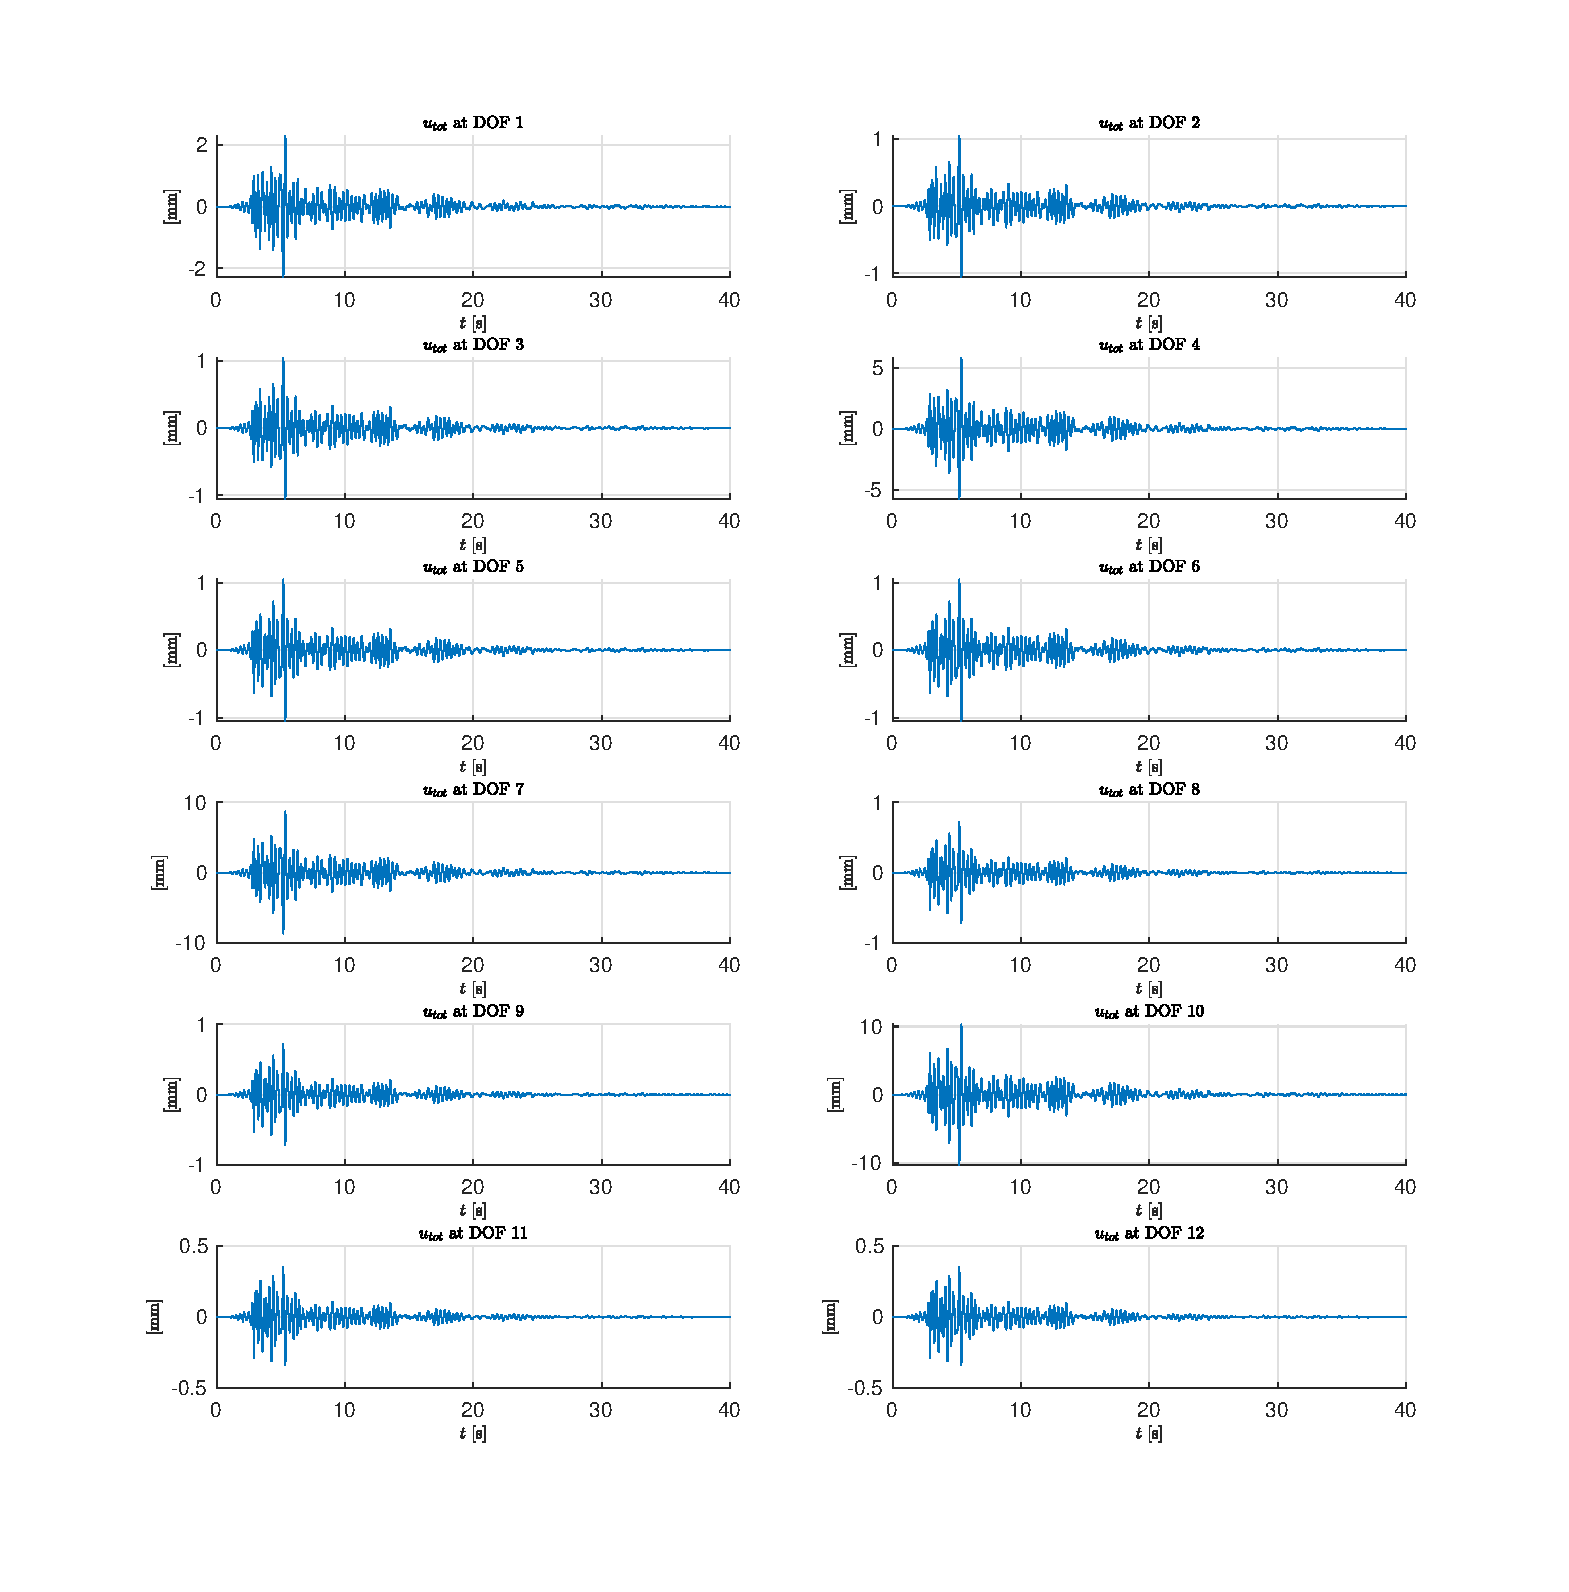
\includegraphics[width=16cm]{LR_TH_Utot_x.eps}
    \caption{Displacement of the Structure in the (X,Z) plane determined using the time history analysis}
    \label{fig:LR_TH_Utot_x}
\end{figure}
\newpage
\begin{figure} [h]
    \centering
    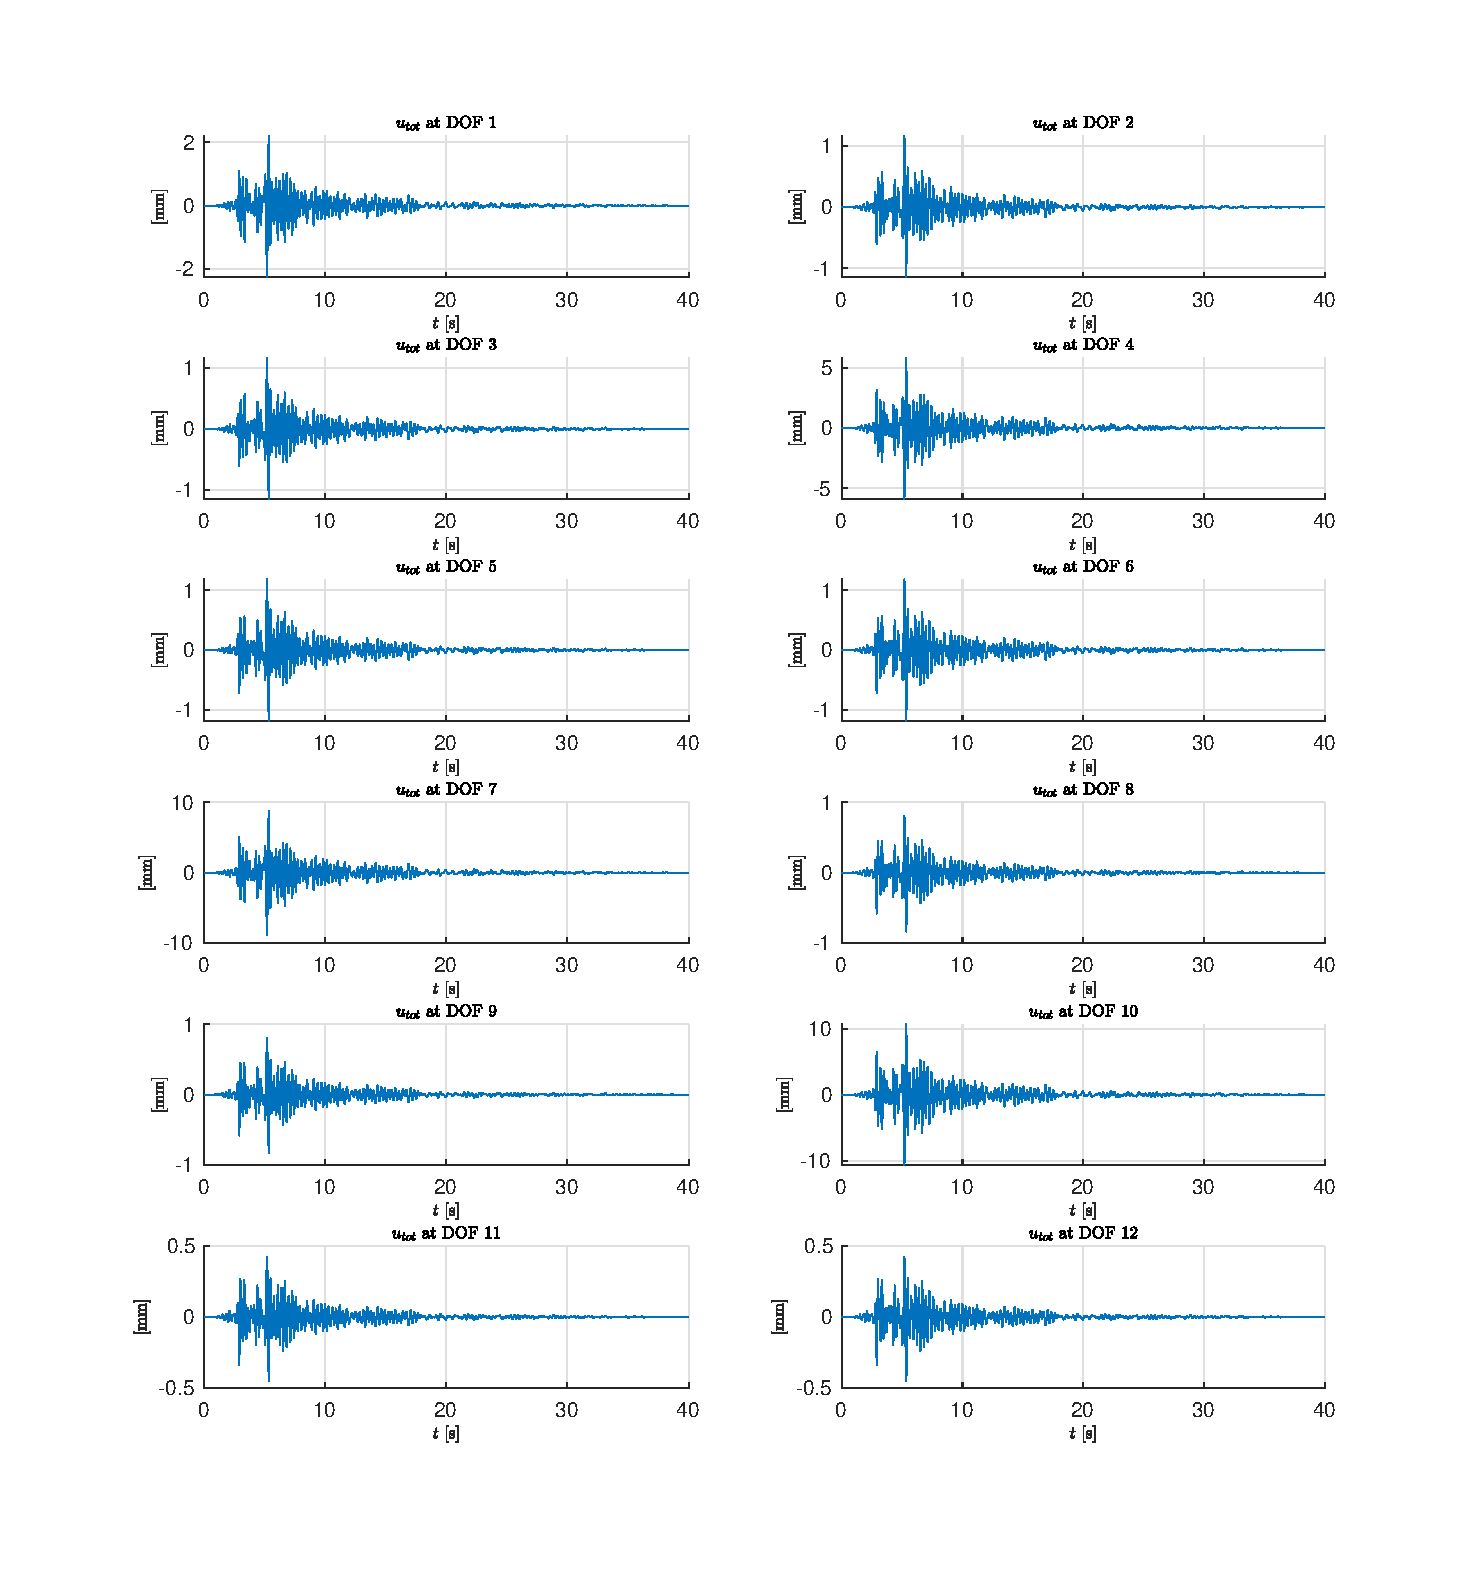
\includegraphics[width=16cm]{LR_TH_Utot.eps}
    \caption{Displacement of the Structure in the (Y,Z) plane determined using the time history analysis}
    \label{fig:LR_TH_Utot}
\end{figure}
\section{High Rise Building}
\paragraph{}The time history analysis of the high rise building was determined in using the same Duhamel integration process shown earlier. For the high rise building the height was divided into four equal sections and the response of the building was determine at those four different heights, the results of which are shown in \textsc{Figure}\,\ref{fig:HR_TH_X} and \textsc{Figure}\,\ref{fig:HR_TH_Y}. When analyzing these figures it should be noted that the results were not normalized, and so attention should be drawn to the y-axis as the scales of all the results vary. Moving clockwise through the plots in both figures and starting in the upper right corner, the results at the bottom of the high rise building can be seen. These results show that as the height of the building increases so does the displacement induced by the strong ground motions. These results also vary between the (X,Z) and (X,Y) planes. The larger displacement is seen in the (Y,Z) plane, this can likely be attributed to the moment of inertia of the structure as it is easier for the building to bend in the Y direction. The results of the maximum displacements in both the (X,Z) and (Y,Z) planes have been summarized in \textsc{Table}\,\ref{tab:maximum total displacement HR TH}
\begin{table}[h]
    \centering
    \begin{tabular}{c|c|c}
    Height &    $U_{tot,X}$ $[m]$ & $U_{tot,Y}$ $[m]$\\
         \hline
     $0$ &  $0.0048$ & $0.0078$\\
      $H/3$ & $0.0116$ & $0.0139$\\
      $2H/3$ &  $0.0201$ & $0.0216$\\
      $H$ &  $0.0315$ & $0.0329$\\
    \end{tabular}
    \caption{Maximum Total Displacements in the High Rise Building}
    \label{tab:maximum total displacement HR TH}
\end{table}
\begin{figure} [h]
    \centering
    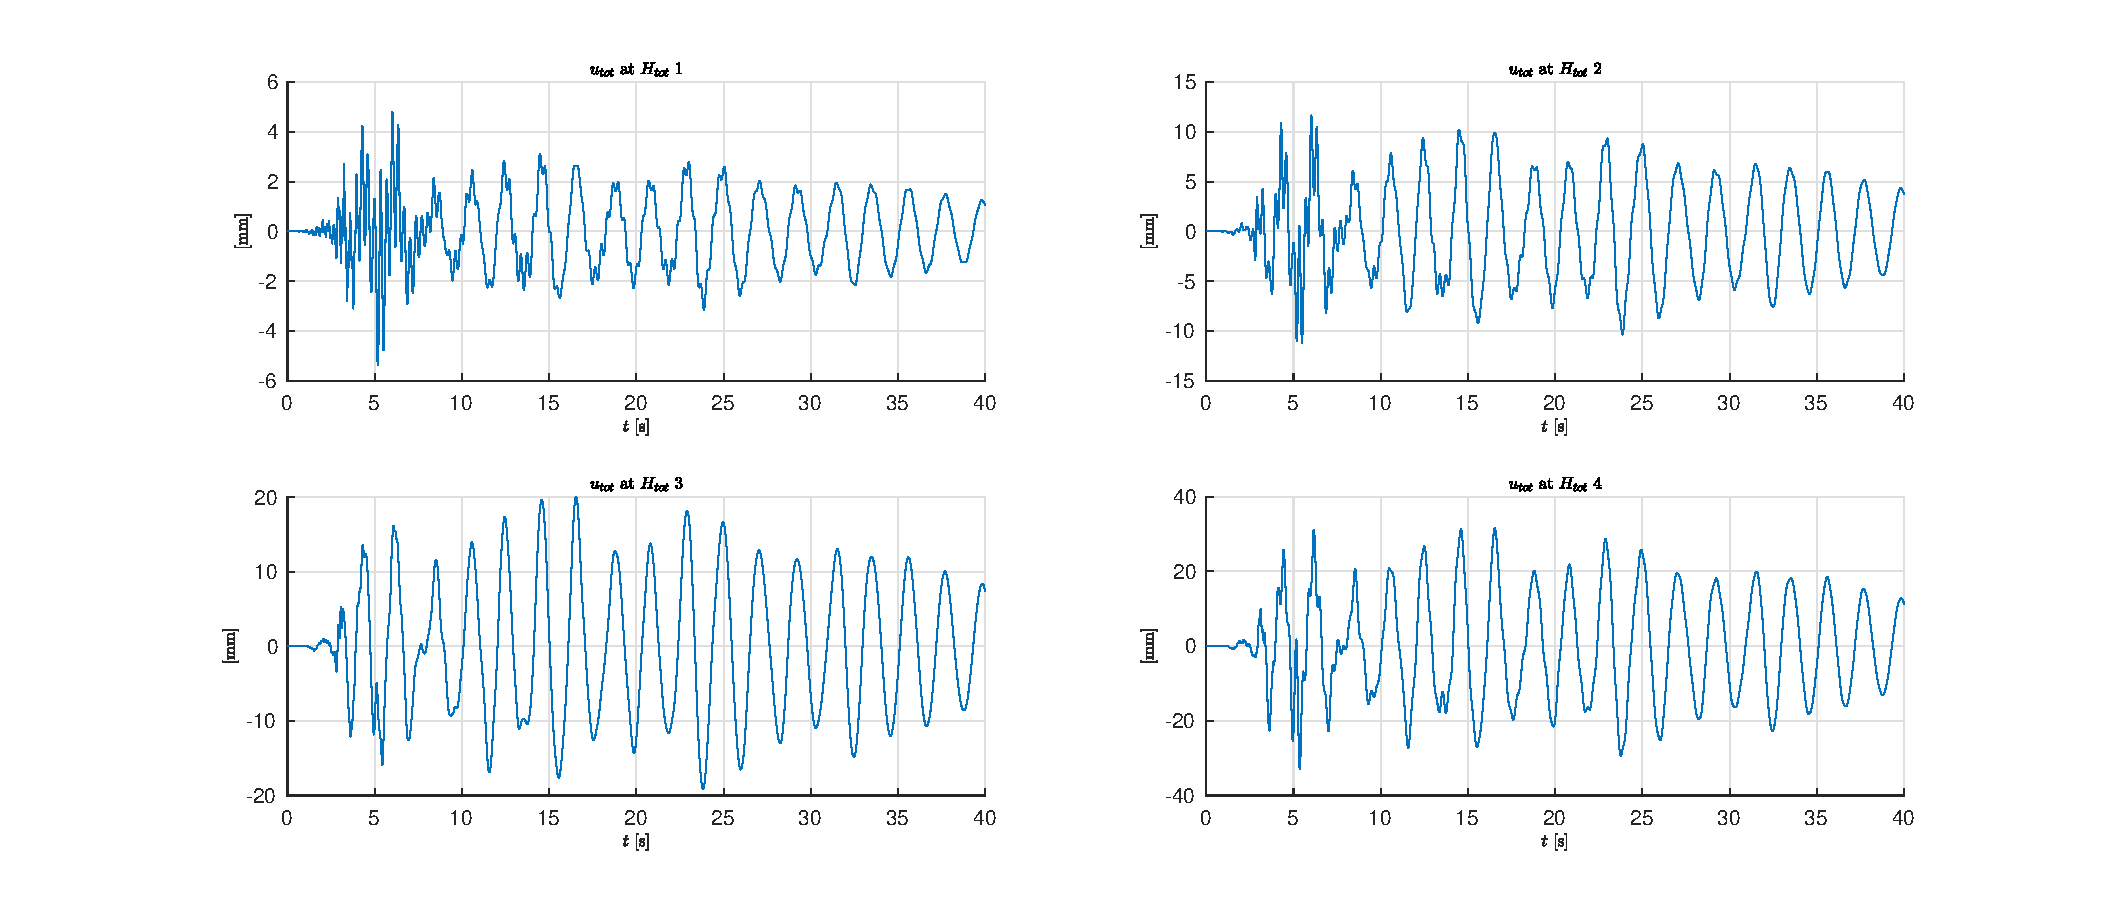
\includegraphics[width=16cm]{HR_TH_X.eps}
    \caption{Resulting Displacements of the Time History Analysis in the (X,Z) plane of the High Rise Building}
    \label{fig:HR_TH_X}
\end{figure}
\begin{figure} [h]
    \centering
    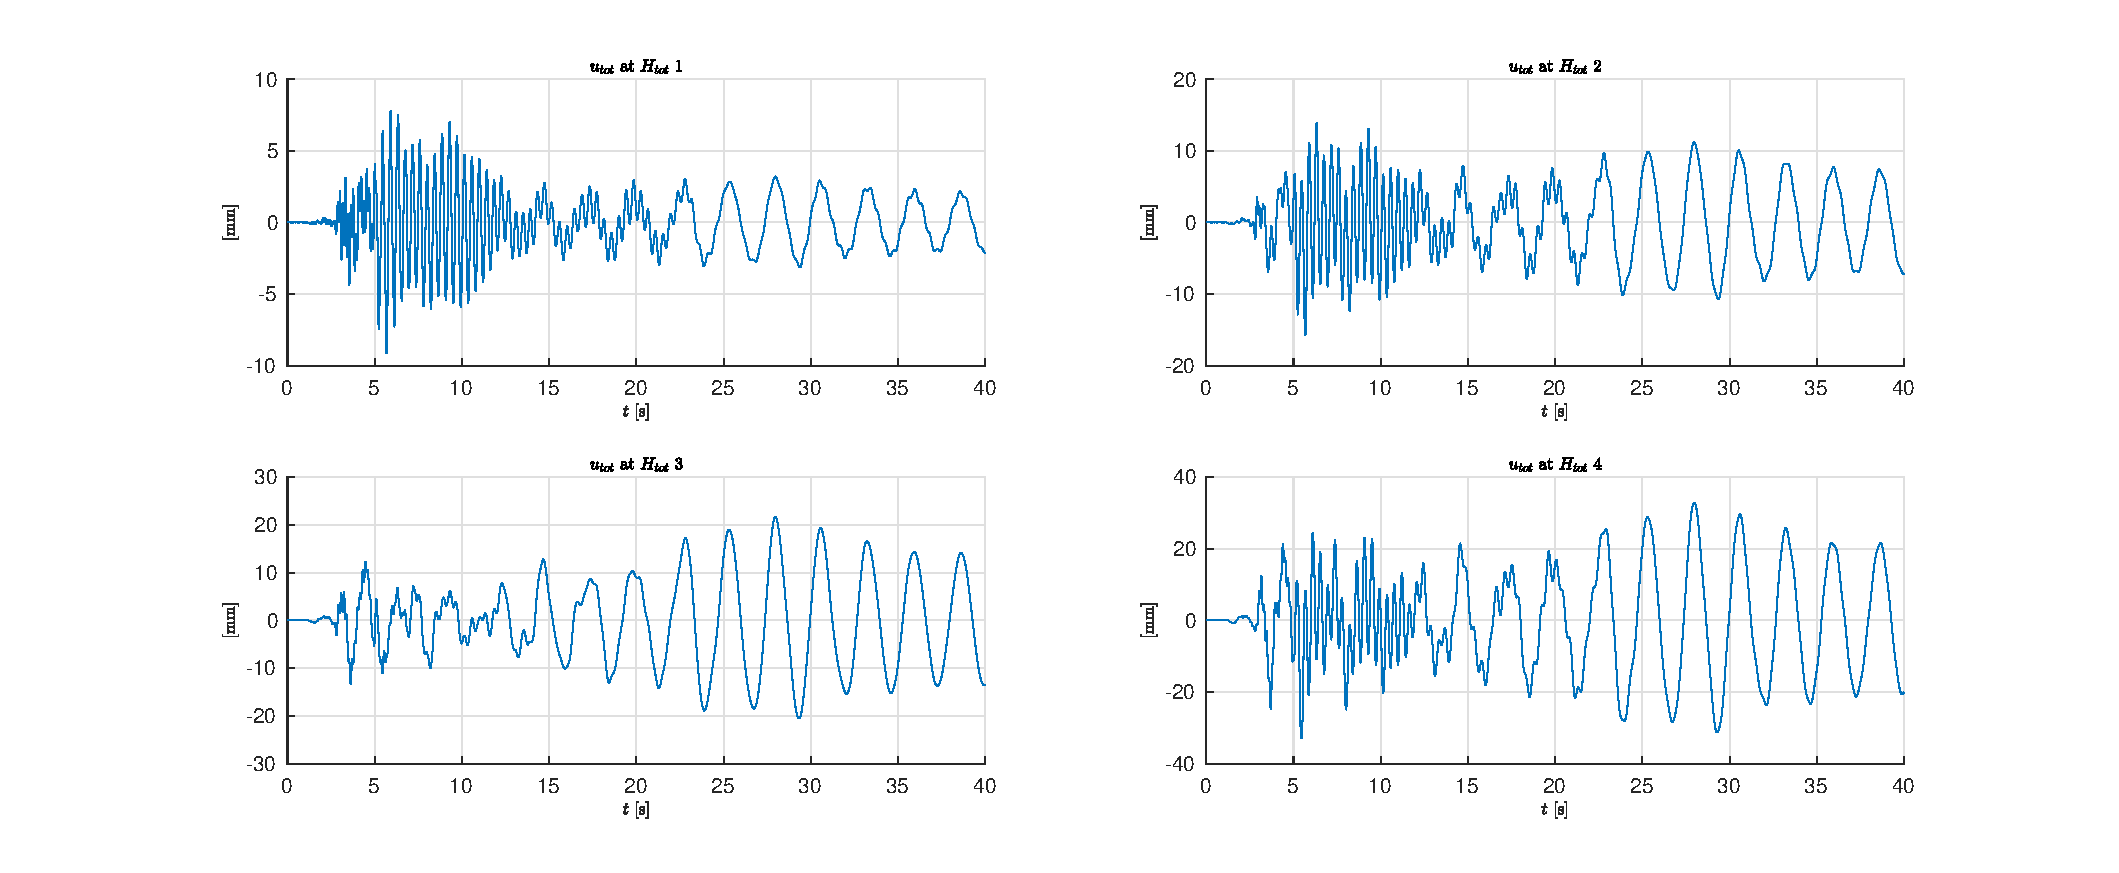
\includegraphics[width=16cm]{HR_TH_Y.eps}
    \caption{Resulting Displacements of the Time History Analysis in the (Y,Z) plane of the High Rise Building}
    \label{fig:HR_TH_Y}
\end{figure}
\chapter{Structural Response Discussion}
\paragraph{}This chapter of the report is dedicated the discussing and comparing the results of the response of the structure produced using the modal response spectrum analysis and the time history analysis. The both analyses are linear dynamic assessments that are used in industry, but there are benefits and disadvantages associated with each. 
\paragraph{}As discussed in course lectures, the modal response spectrum analysis the the analysis method that is most used in industry. The spectrum can not determine the inelastic displacements within a structure, so it is best used for structures who's behavior will remain within the elastic range. On the other hand, the time history analysis can be used for a wide range of structures. Unlike the modal response spectrum analysis it is appropriate for structures who's behavior is elastic or inelastic. On the contrary, the time history analysis is more complicated which is one of the reasons why it is less used in industry.
\section{Low Rise Building}
\section{High Rise Building}
\paragraph{}The displacement results produced from the modal response spectrum analysis and the time history analysis of the high rise building are shown in \textsc{Table}\,\ref{tab:total displacements HR} and \textsc{Table}\,\ref{tab:maximum total displacement HR TH}. Comparing these results it can be seen that the modal response spectrum has produced displacement values that are in some cases a magnitude larger that that of the results of the time history analysis. 
\section{Conclusion}
\paragraph{}The comparison of results of displacements and forces from the modal response spectrum analysis and time history analysis brought forward an interesting discussion. From this discussion in can be concluded that both analyses have their own benefits and disadvantages. With this being said it is recommended that for the seismic design of buildings both analyses be used.  
%design verification
\chapter{Design Verification}
\paragraph{}The design verification will only be applied to the low rise structure. It has been assumed that the building has ductile non-structural elements for this assesement. The design verification of the building includes an assessment of all the forces impacting the structure, both static and dynamic, and how the interaction of these forces during strong ground motion will impact the structure. Also included in the design verification is an assessment of the damage limitation state. This is done by determining interstorey drift for each storey in both planes of the low rise building. From which the interstorey drift sensitivity coefficient can be calculated to ensure that the drifts occurring during strong ground motions meet the standards set out by Eurocode 8. The ultimate limit state has also been determined to verify the design and includes the moment resistance capacities of the members of the structure.
\section{Design Section Forces}
\paragraph{}The verification of design of this structure includes combining the seismic section forces determined from the structural response with that of the other forces acting on the building. Prior to this, the static forces on the low rise building must be determined. This has been done using a finite element modeling program, Autodesk Robot. The 2D frame was modeled in the (X,Z) direction, using the programs specifications for reinforced concrete, and concrete material concrete 30. The dead loads and live loads were applied to the structure and the results were analyzed. A visual representation of the bending moments is shown in \textsc{Figure}\,\ref{fig:I.4: Autodesk Forces 1}, and \textsc{Figure}\,\ref{fig:I.4: Autodesk Forces 2}.
\begin{figure}
\begin{minipage}{0.49\textwidth}
    \centering
    \includegraphics[width=6cm]{Nat_My.JPG}
\end{minipage}
\begin{minipage}{0.49\textwidth}
    \centering
    \includegraphics[width=6cm]{Nat_Fx.JPG}
\end{minipage}
    \caption{Low Rise Structure showing Resulting Bending Moments and Shear Forces in the (X,Z) direction  modeled in Autodesk Robot}
      \label{fig:I.4: Autodesk Forces 1}
\end{figure}

\begin{figure}
\begin{minipage}{0.49\textwidth}
   \centering
    \includegraphics[width=6cm]{Nat_My_Y.JPG}
\end{minipage}
\begin{minipage}{0.49\textwidth}
   \centering
    \includegraphics[width=6cm]{Nat_Fx_Y.JPG}
        \label{fig:I.4: Autodesk Forces 2}
\end{minipage}
  \caption{Low Rise Structure showing Resulting Bending Moments and Shear Forces in the (Y,Z) direction  modeled in Autodesk Robot}
\end{figure}
\paragraph{}The output data gathered from this program gave the static forces of the building for the impacts of the live load and both dead loads applied to the structure. These three static forces were combined to creating the total static forces of the building and have been presented in \textsc{Table}\,\ref{tab:static forces x} and \ref{tab:static forces y}. The first four columns of this table given the shear force and bending moment that correspond to those shown in \textsc{Figure}\,\ref{fig: I.1 - DOF} for the local system. The last two columns show the axial forces being imposed on the building. These forces act downwards in the Z direction and are needed to determine the seismic load of the structure. From these figures and tables it is evident that the static forces within the building decrease inversely with the height. This is expected as the loads on the top of the building are carried by the entire structure, while the loads imposed on the first floor are only carried by the bottom most columns of the structure.
\begin{table}[h]
    \centering
    \begin{tabular}{c|c|c|c|c|c|c}
     Element & $F_1\,[N]$ & $F_2 \,[N]$ & $M_3 \,[Nm]$ & $M_4\, [Nm]$ & $A_5 \,[N]$ & $A_6\, [N]$ \\
         \hline
    $1$ & $105140$ & $117410$ & $-33750$ & $-26050$ & $-3080$ & $-3080$ \\
    $2$ & $85730$ & $73470$ & $-19190$ & $-26590$ & $-2960$ & $-2960$ \\
    $3$ & $54070$ & $41800$ & $-12040$ & $-18280$ & $-2500$ & $-2500$ \\
    $4$ & $10130$ & $22390$ & $-7590$ & $-3730$ & $-310$ & $-1540$ \\
    $5$ & $10130$ & $22390$ & $7590$ & $3730$ & $1540$ & $1540$ \\
    $6$ & $41800$ & $54070$ & $18280$ & $12040$ & $2500$ & $2500$ \\
    $7$ & $73470$ & $85730$ & $26590$ & $19190$ & $2960$ & $2960$ \\
    $8$ & $105140$ & $117410$ & $33750$ & $26050$ & $3080$ & $3080$ \\
    $9$ & $-19410$ & $19410$ & $-14550$ & $-14550$ & $120$ & $120$ \\
    $10$ & $-19410$ & $19410$ & $-14550$ & $-14550$ & $460$ & $460$ \\
    $11$ & $-19410$ & $19410$ & $-14550$ & $-14550$ & $960$ & $960$ \\
    $12$ & $-10130$ & $10130$ & $-7590$ & $-7590$ & $1540$ & $1540$ \\
    \end{tabular}
    \caption{Static Forces of the Low Rise Building in the (X,Z) Plane}
    \label{tab:static forces x}
\end{table}
\begin{table}[h]
    \centering
    \begin{tabular}{c|c|c|c|c|c|c}
     Element & $F_1 \,[N]$ & $F_2 \,[N]$ & $M_3\, [Nm]$ & $M_4 \,[Nm]$ & $A_5 \,[N]$ & $A_6\, [N]$ \\
         \hline
    $1$ & $105140$ & $117410$ & $-29560$ & $-20010$ & $-3810$ & $-3810$ \\
    $2$ & $85730$ & $73470$ & $-15000$ & $-24160$ & $-3670$ & $-3670$ \\
    $3$ & $54070$ & $41800$ & $-9610$ & $-17360$ & $-3090$ & $-3090$ \\
    $4$ & $10130$ & $22390$ & $-7590$ & $-2800$ & $-390$ & $-1910$ \\
    $5$ & $10130$ & $22390$ & $7590$ & $2800$ & $1910$ & $1910$ \\
    $6$ & $41800$ & $54070$ & $17360$ & $9610$ & $3090$ & $3090$ \\
    $7$ & $73470$ & $85730$ & $24160$ & $15000$ & $3670$ & $3670$ \\
    $8$ & $105140$ & $117410$ & $29560$ & $20010$ & $3810$ & $3810$ \\
    $9$ & $-19410$ & $19410$ & $-19410$ & $19410$ & $160$ & $160$ \\
    $10$ & $-19410$ & $19410$ & $-19410$ & $19410$ & $560$ & $560$ \\
    $11$ & $-19410$ & $19410$ & $-19410$ & $19410$ & $1180$ & $1180$ \\
    $12$ & $-10130$ & $10130$ & $-10130$ & $10130$ & $1910$ & $1910$ \\
    \end{tabular}
    \caption{Static Forces of the Low Rise Building in the (Y,Z) Plane}
    \label{tab:static forces y}
\end{table}
\paragraph{}With the total static forces of the building obtained, the total forces being applied on the building can now be determined by combining these static forces and the dynamic forces induced by the strong ground motions. For this, the modal section forces determining using the modal response spectrum and CQC modal combination method have been chosen as these are the most conservative values, in doing so gives the greatest safety factor. The results of which have been summarized into \textsc{Table}\,\ref{tab:dynamic and static x} and \ref{tab:dynamic and static x}.
\begin{table}[h]
    \centering
    \begin{tabular}{c|c|c|c|c}
      Element & $F_1 \,[kN]$ & $F_2 \,[kN]$ & $M_3\, [kNm]$ & $M_4 \,[kNm]$  \\
         \hline
       $1$ & $133.92$ & $146.19$ & $-13.63$ & $25.86$ \\
       $2$ & $111.54$ & $99.28$ & $13.37$ & $5.48$ \\
       $3$ & $73.30$ & $61.03$ & $16.96 $ & $0.98$ \\
       $4$ & $19.71$ & $31.97$ & $9.80$ & $3.17 $ \\
       $5$ & $19.71$ & $31.97$ & $24.98$ & $10.63$ \\
       $6$ & $61.03$ & $73.30$ & $47.28$ & $31.30$ \\
       $7$ & $99.28$ & $111.54$ & $59.15$ & $51.26$ \\
       $8$ & $133.92$ & $146.19$ & $53.87$ & $77.96$ \\
       $9$ & $3.70$ & $42.52 $ & $37.44$ & $37.44$ \\
       $10$ & $3.38$ & $42.20$ & $36.73$ & $36.73$ \\
       $11$ & $-3.81$ & $35.01$ & $20.55$ & $20.55$ \\
       $12$ & $-2.55$ & $17.71$ & $9.46$ & $9.46$ \\
    \end{tabular}
    \caption{Result of Combining the Static and Dynamic Forces Acting Upon the Low Rise Building in the (X,Z) Plane}
    \label{tab:dynamic and static x}
\end{table}
\begin{table}[h]
    \centering
    \begin{tabular}{c|c|c|c|c}
      Element & $F_1 \,[kN]$ & $F_2 \,[kN]$ & $M_3\, [kNm]$ & $M_4 \,[kNm]$  \\
         \hline
       $1$ & $138.61 $ & $150.88$ & $-13.39$ & $47.80$ \\
       $2$ & $115.85$ & $103.59 $ & $21.70 $ & $14.69$ \\
       $3$ & $76.75 $ & $64.48 $ & $ 26.34$ & $ 3.88$ \\
       $4$ & $ 21.71$ & $33.97$ & $ 15.39 $ & $4.35$ \\
       $5$ & $21.71$ & $33.97$ & $30.57$ & $9.95$ \\
       $6$ & $ 64.48$ & $76.75$ & $53.31$ & $30.85$ \\
       $7$ & $103.59$ & $115.85 $ & $60.86$ & $53.85$ \\
       $8$ & $138.61$ & $150.88$ & $45.73 $ & $87.82$ \\
       $9$ & $4.73 $ & $43.55$ & $34.91 $ & $73.73$ \\
       $10$ & $5.80$ & $44.62$ & $37.32$ & $76.14$ \\
       $11$ & $-1.23$ & $37.60 $ & $21.51 $ & $60.33$ \\
       $12$ & $-0.08 $ & $20.18$ & $12.47 $ & $32.73$ \\
    \end{tabular}
    \caption{Result of Combining the Static and Dynamic Forces Acting Upon the Low Rise Building in the (X,Z) Plane}
    \label{tab:dynamic and static x}
\end{table}
\subsection{Eurocode Seismic Load Combination}
\paragraph{}In order to determine the total load on the building the seismic load combination rules as determined by the Eurocode must be followed. Part 1 of Eurocode 8 states that \textsc{Equation}\,\eqref{eq:I.4 EC governing eq} is to be used for the combination of concurrent loads in seismic design situations \cite{EC8}. 
\begin{equation}
    E=\sum_{j\geq1} G_{k,j}\,\pm\,P\,\pm\,A_{ED}\,\pm\,\sum_{i\geq1}\Phi_{2,i}\,Q_{k,i}
    \label{eq:I.4 EC governing eq}
\end{equation}
\paragraph{}Where,
\begin{itemize}
   \begin{small}
    \item $G_{k,j}$ is the permanent actions imposed on the building provided by the static forces $[N]$
    \item $P$ is the prestressing of structural members 
    \item $A_{ED}$ is the design seismic actions provided by the total modal forces determined in the modal response of the building
    \item $\Phi_{2,i}\,Q_{k,i}$ is representative of the variable actions 
     \item $\pm$ whichever action leads to an increase in the total seismic load is chosen 
   \end{small}
\end{itemize}
\paragraph{}This governing equation must be determined for all three axis of the structure for the purpose of the seismic load combination. This combination of loads not only considers the static and dynamic loads of the plane being studied, but also considers the loads from the other directions that may additionally be imposed on the plane of study during strong ground motions, by considering $30\%$ of these loads. This combination is governed by \textsc{Equation}\,\eqref{eq:I.4 seismic load combinations}. The resulting seismic loads have been presented in \textsc{Table}\,\ref{tab:EC seimic load x} and \ref{tab:EC seimic load y}
\begin{equation}
    E=E_x\,\pm\,0.3\,E_y\,\pm\,0.3\,E_z
    \label{eq:I.4 seismic load combinations}
\end{equation}
\paragraph{}Where,
\begin{itemize}
    \begin{small}
    \item $E$ is the total seismic load $[N]$
    \item $E_x$ is the total static and dynamic loads in the (X,Z) plane $[N]$
    \item $E_x$ is the total static and dynamic loads in the (Y,Z) plane $[N]$
    \item $E_z$ is the static axial forces from the Z direction $[N]$
    \item $\pm$ whichever action leads to an increase in the total seismic load is chosen 
    \end{small}
\end{itemize}
\begin{table}[h]
    \centering
    \begin{tabular}{c|c|c|c|c}
    Element & $F_1 \,[kN]$ & $F_2 \,[kN]$ & $M_3\, [kNm]$ & $M_4 \,[kNm]$  \\
         \hline
    $1$ & $242.27$ & $258.22$ & $57.15 $ & $106.97$ \\
    $2$ & $194.06$ & $178.12$ & $67.64$ & $57.64$ \\
    $3$ & $125.09$ & $109.14$ & $53.62$ & $30.91$ \\
    $4$ & $35.98$ & $ 51.92$ & $24.17 $ & $14.23$ \\
    $5$ & $35.98$ & $51.92$ & $43.91$ & $23.37$ \\
    $6$ & $109.14$ & $125.09$ & $92.04$ & $69.32$ \\
    $7$ & $178.12$ & $194.06 $ & $125.17$ & $115.17$ \\
    $8$ & $242.27 $ & $ 258.22$ & $134.35$ & $171.07$ \\
    $9$ & $5.12$ & $55.58 $ & $47.91 $ & $59.56$ \\
    $10$ & $5.12$ & $55.59$ & $47.92$ & $59.57$ \\
    $11$ & $-3.44$ & $46.29$ & $27.00$ & $38.64$ \\
    $12$ & $ -2.53 $ & $23.76$ & $13.20 $ & $ 19.28$ \\
    \end{tabular}
    \caption{Seismic Loads of the Low Rise Building in the (X,Z) Plane Determined Using Eurocode Seismic Load Combination Rules}
    \label{tab:EC seimic load x}
\end{table}
\begin{table}[h]
    \centering
    \begin{tabular}{c|c|c|c|c}
    Element & $F_1 \,[kN]$ & $F_2 \,[kN]$ & $M_3\, [kNm]$ & $M_4 \,[kNm]$  \\
         \hline
    $1$ & $245.55 $ & $261.50$ & $57.47 $ & $122.33$ \\
    $2$ & $197.08$ & $181.14$ & $73.47$ & $64.10$ \\
    $3$ & $127.50$ & $111.55$ & $60.19$ & $32.94$ \\
    $4$ & $37.38$ & $53.32$ & $28.09$ & $15.05$ \\
    $5$ & $37.38 $ & $53.32$ & $47.82$ & $22.89$ \\
    $6$ & $111.55$ & $127.50$ & $96.25$ & $69.00$ \\
    $7$ & $181.14 $ & $197.08$ & $126.37$ & $116.99$ \\
    $8$ & $245.55$ & $261.50 $ & $128.66$ & $177.98$ \\
    $9$ & $5.84$ & $56.31$ & $46.14$ & $84.96$ \\
    $10$ & $6.82$ & $57.28 $ & $48.34 $ & $87.16$ \\
    $11$ & $-0.08$ & $48.10$ & $27.67$ & $66.49$ \\
    $12$ & $0.68$ & $25.49$ & $15.31$ & $35.57$ \\
    \end{tabular}
    \caption{Seismic Loads of the Low Rise Building in the (Y,Z) Plane Determined Using Eurocode Seismic Load Combination Rules}
    \label{tab:EC seimic load y}
\end{table}
\section{Damage Limitation State}
\paragraph{}In order to meet the damage limitation performance requirement, the interstory drift limitations must be met. To comply with this, the criterion shown in \textsc{Equation}\,\eqref{eq:I.4 - interstory drift criterion} needs to be fulfilled. The reduction factor is a Eurocode 8 recommendation that takes into consideration the lower return period of the earthquake. The prescribed values are based on the importance class of the structure being assessed. For this verification a value of $0.5$ has been used in compliance with the Eurocode 8 recommendation for importance class II. Using the relationship stated in \textsc{Equation}\,\eqref{eq:I.4 - interstory drift criterion} the maximum interstory drift is $0.75\%$, specifically considering the importance class and interstorey height of this low rise building it is a value of $0.0075m$. The results of the interstorey drift of the low rise building have been presented in \textsc{Table}\,\ref{tab:interstorey drift}. These values have been multiplied by the reduction factor to take the importance class of the structure into consideration.
\begin{equation}
    d_r\,v\geq0.0075\,h
    \label{eq:I.4 - interstory drift criterion}
\end{equation}
\paragraph{}Where,
\begin{itemize}
\begin{small}
    \item $d_r$ is the design interstorey drift $[m]$
    \item $h$ is the story height $[m]$
    \item $v$ is the reduction factor $[-]$
\end{small}
\end{itemize}
\begin{table}[h]
    \centering
    \begin{tabular}{c|c|c}
       Storey  & (X,Z) plane $[m]$ & (Y,Z) plane $[m]$ \\
       \hline
       $1$  & $0.0039$ & $0.0039$ \\
       $2$ & $0.0058$ & $0.0058$ \\
       $3$ & $0.0047$ & $0.0049$ \\
       $4$ & $0.0027$ & $0.0030$ \\
    \end{tabular}
    \caption{Results of Interstorey Drift between Stories 1,2, and 3 in the (X,Z) and (Y,Z) planes}
    \label{tab:interstorey drift}
\end{table}
\paragraph{}The results of the interstorey drift calculations show that the drift experienced by the building is slightly larger in the (Y,Z) plane than the (X,Z) plane. This outcome can be explained by the moment of inertia of the low rise structure, due to the geometry of the columns bending is easier in the (Y,Z) plane and therefore the interstorey drift is larger in this plane. Assessing the results, it can also be seen that the drift is largest at the second and third floors of the building and smaller at the first floor and roof. This is because the columns below the first floor are attached to the fixed points on the ground so the drift at this level is expected to be smaller. At the roof level the drift is also expected to be small as the movements of the building are governed by the movement of the lower floors as they carry more weight increasing their moment of interia. Therefore the drift is expected to decrease as the height above this storey increases, as the weight of the building
\subsection{Interstorey Drift Sensitivity}
\paragraph{} The interstorey drift sensitivity coefficient is a measure used to determine the severity of the drift occurring in the structure. Because buildings vary in geometry, mass, and loads this coefficient can be used as a unit less comparison of the interstorey drift of a structure, as the severity is dependent on more than just the displacement occurring. It takes into account both dead loads, live loads, and seismic forces imposed on the building, as well as the inherent properties of the structure such as its mass and height. The interstorey drift sensitivity coefficient needs to be calculated to determine if second order effects should be considered. The coefficient must be smaller than $0.01$ for these effects to be ignored. The coefficient is calculated using \textsc{Equation}\,\eqref{eq:I.4 - Ultimate Limit State Verification}.
\begin{equation}
    \theta=\dfrac{P_{tot}\,d_r}{V_{tot}\,h}
    \label{eq:I.4 - Ultimate Limit State Verification}
\end{equation}
\paragraph{}Where,
\begin{itemize}
\begin{small}
    \item $\theta$ is the interstorey drift sensitivity coefficient
    \item $P_{tot}$ is the total gravity load at and above the storey
    \item $d_r$ is the design interstorey drift
    \item $V_{tot}$ is the total seismic storey shear
    \item $h$ is the storey height
\end{small}
\end{itemize}
\paragraph{}The product of which can be found in \textsc{Table}\,\ref{tab:interstorey drift}. The results show that while considering other factors that effect the behavior of the building, the sensitivity is highly dependent on the interstorey drift of the low rise building. The results follow the same trends as that of the interstorey drift for the same reasons as explained previously.
\begin{table}[h]
    \centering
    \begin{tabular}{c|c|c}
    Storey  & (X,Z) plane $[-]$ & (Y,Z) plane $[-]$ \\
       \hline
        $1$ & $0.0039$ & $0.0039$ \\
        $2$ & $0.0058$ & $0.0058$ \\
        $3$ & $0.0047$ & $0.0049$ \\
        $4$ & $0.0027$ & $0.0030$ \\
    \end{tabular}
    \caption{Interstorey Drift Sensitivity Coefficients in both the (X,Z) and (Y,Z) planes}
    \label{tab:interstorey drift}
\end{table}
\section{Ultimate Limit State}
\subsection{Moment Resistance Capacities}

\section{General Requirements Verification}
\subsection{Moment Resistance Capacities}
\paragraph{}The ductility class of the building is high as the behavioral factor is greater than $1.5$. 
\subsection{Behavior Factor}
%\paragraph{}The behavior factor used for the modal response analysis was provided as given in \textsc{Table}\,\ref{tab: Specifications - Design LowRB } and \textsc{Table}\,\ref{tab: Specifications - Design HighRB} as 4.0, and 1.0 for the low rise, and high rise buildings respectively. In Eurocode 8 the behavioral factor is given by \textsc{Equation}\,\eqref{eq:I.4 - behavioral factor EU8} below.
%\begin{equation}
 %   q=q_0\,k_w
  %  \label{eq:I.4 - behavioral factor EU8}
%\end{equation}
%\paragraph{}Where,
%\begin{itemize}
%\begin{small}
 %   \item $q$ is the behavioral factor $[-]$
  %  \item $q_0$ is the basic q factor $[-]$
   % \item $k_w$ is the wall failure mode factor $[-]$
%\end{small}
%\end{itemize}
%\paragraph{}The basic q factor here takes the ductility class of the reinforced concrete structure into consideration. Values of the basic q factor increase with increased ductility of the reinforced concrete. This is an important factor as the ductility of the reinforced concrete will affect the performance of a structure during strong ground motions. The wall failure mode factor accounts for the structural system within the walls of the  building. Aspects affecting this factor include if the building is single or multistory, and the frame systems within the structure. 
\subsubsection{Recomendations}
\begin{itemize}
    \item increasing reinforcement in bottom of beams and outer edges of concrete 
    \item Increase symmetry by changing dimensions of columns
    \item uniform geometry
\end{itemize}
\chapter{Soil - Structure Interaction}
\paragraph{}This section of the report will focus on the soil-structure interaction between a predominately soft-firm cohesionless soil and the low rise building. This soil type is refered to as soil type D in Eurocode 8 and its parameters have been provided including its shear wave velocity, density, and poisson's ratio in \textsc{Table}\,\ref{tab: specifications - soil}. 
\paragraph{}The soil-structure interaction analysis is a combination of the kinematic interaction of the massless foundation and soil, and the inertial interaction of the effective mass of the structure and the underlying soil. The inertial interaction assesses the system as a simple dynamic system composed of a mass, a spring, and a dashpot. From this, the dynamic soil stiffness and radiation dashpot coefficients can be derived. With these properties, both the equivalent frequency and damping ratio of the soil-structure system are determined. These parameters are used to obtain the modal displacements and modal section forces which will reflect the implications of the soil-structure interaction during strong ground motions.
\paragraph{}It is important to note the assumptions made in conducting the analysis of the interaction between the subsurface structure and the low rise building. While unrealistic, it has been assumed that the soil layer above the bedrock is completely homogeneous. Additionally, it has been assumed that the underlying bed rock is a flat and rigid surface. These assumptions deviate from reality as a uniform $23m$ thick layer is extremely uncommon. This section of the report will outline the necessary theory behind the soil-structure interaction, but in real world applications it would be necessary to perform further geological site investigations. This would include a drilling plan or test pits to determine subsurface conditions which should then be modeled before conducting this assessment. 

\section{Part I}
\paragraph{}The first part of determining the soil structure interaction is taking the system from a MDOF system to a SDOF system. To do this one must start by first looking at, \textsc{Equation}\,\eqref{eq:I.5 base shear force MDOF} and \textsc{Equation}\,\eqref{eq:I.5 base overturning moment MDOF}. These equations govern the relationship between the base shear force and the base overturning moment and their respective dependent effective modal mass and modal height for a MDOF system. 
\begin{equation}
    V_{bi}(t)=V_{bi}^{st}\,A_i(t)
    \label{eq:I.5 base shear force MDOF}
\end{equation}
\begin{equation}
    M_{bi}(t)=M_{bi}^{st}\,A_i(t)
    \label{eq:I.5 base overturning moment MDOF}
\end{equation}
\paragraph{}The modal static response to the base shear force and the modal static response to the base overturning moment can also been defined by \textsc{Equation}\,\eqref{eq:I.5 modal static response to base shear force}, and \textsc{Equation}\,\eqref{eq:I.5 modal static response to base overturning moment}. This relationship equates the MDOF system on the left hand side of the equation to the SDOF system on the right hand side.
\begin{equation}
    V_{bi}^{st}=\sum^N_{j=1}\,s_{ji}=M^*_i
    \label{eq:I.5 modal static response to base shear force}
\end{equation}
\begin{equation}
    M_{bi}^{st}=\sum^N_{j=1}\,h_j\,s_{ji}=M^*_i\,h_i^*
    \label{eq:I.5 modal static response to base overturning moment}
\end{equation}
\paragraph{}So, with the relationships between the static responses to the base shear forces and the over turning moments and the effective mass and effective height, we can substitute the latter back into the equations given for the base shear force and overturning moment for the SDOF system. The result of which has been provided in \textsc{Equation}\,\eqref{eq:I.5 base shear force} and \textsc{Equation}\,\eqref{eq:I.5 base overturning moment}.
\begin{equation}
    V_{bi}(t)=M^*_{bi}\,A_i(t)
    \label{eq:I.5 base shear force}
\end{equation}
\begin{equation}
    M_{bi}(t)=h_i^*\,V_{bi}(t)
    \label{eq:I.5 base overturning moment}
\end{equation}
\paragraph{}Now that the relationship between the base shear force and overturning moment and the effective mass and height has been determined, the system can be taken from a MDOF to a SDOF. This is because the base shear force and overturning moment of a SDOF is equal to that of a MDOF system. Referring back to earlier in the report when the effective modal mass of the low rise building was determined, the equation has been shown again here in \textsc{Equation}\,\eqref{eq:I.1 - Effective Modal Mass - Low Rise - for SSI} \cite{textbook}.
\begin{equation}
    M_{eff,i} = MPF_i\,\phi_i^T\,M\,r
    \label{eq:I.1 - Effective Modal Mass - Low Rise - for SSI}
\end{equation}
\paragraph{}By substituting the base shear effective mass for the effective mass in this equation, the effective mass of the SDOF system can be determined using\textsc{Equation}\,\eqref{eq:I.5 SDOF effective mass},
\begin{equation}
    M_i^*=MPF_i\,\phi_i^T\,M\,r
    \label{eq:I.5 SDOF effective mass}
\end{equation}
\paragraph{}Now that the effective mass has been determined, the effective height can be determined from the following relationship \cite{textbook}.
\begin{equation}
    V_{bi}=M_{bi}\,A_i(t)
     \label{eq:I.5: equating heights 1}
\end{equation}
\begin{equation}
    V_{bi}(t)=MPF_i\,\phi_i^T\,M\,r\,A_i(t)
     \label{eq:I.5: equating heights 1}
\end{equation}
\begin{equation}
    V_{bi}=M_n^*\,A_n\,h_n^*\,A_i(t)
\end{equation}
\paragraph{}The property given below then allows the actual height of the building to be substituted into the equation \cite{textbook}.
\begin{equation}
    \sum^N_{i=1}h_i^*\,M^*_i= \sum^N_{i=1}h_j\,m_j
\end{equation}
\paragraph{}Using the relationships for the base shear force and base overturning moment of the SDOF given in \textsc{Equation}\,\eqref{eq:I.5 base shear force}, and \textsc{Equation}\,\eqref{eq:I.5 base overturning moment} it can be substituted to produce the following \cite{textbook}.
\begin{equation}
    M_n^*\,A_n\,h_j^*=M_n^*\,A_n\,h_n^*
\end{equation}
\begin{equation}
    MPF_i\,\phi_i^T\,M\,r\,A_n\,h_j^*=MPF_i\,\phi_i^T\,M\,r\,A_n\,h_n^*
\end{equation}
\paragraph{}Substituting the base shear effective modal mass gives 
\begin{equation}
     h_i^*=\dfrac{h_j\,MPF_i\,\phi_i^T\,M\,r}{MPF_i\,\phi_i^T\,M\,r}
\end{equation}
\paragraph{}Which further simplifies to \textsc{Equation}\,\eqref{eq:I.5 SDOF effective height}, the desired equation for determining the effective height of the SDOF system for the soil structure interaction \cite{textbook}.
\begin{equation}
    h_i^*=\dfrac{h_j^T\,M\,\phi_i}{r^T\,M\,\phi_i}
    \label{eq:I.5 SDOF effective height}
\end{equation}
\paragraph{}Where,
\begin{itemize}
\begin{small}
    \item $V_{bi}(t)$ is the base shear force of mode $(i=1,2,...,12)$ $[N]$
    \item $M_{bi}(t)$ is the base overturning moment of mode $(i=1,2,...,12)$ $[Nm]$
    \item $V_{bi}^{st}$ is the modal static response to the base shear force from mode $(i=1,2,...,12)$ $[N]$
    \item $M_{bi}^{st}$ is the modal static response to the base overturning moment of mode $(i=1,2,...,12)$ $[Nm]$
    \item $A_i(t)$ is the psuedo acceleration $[m/s^2]$
    \item $M^*_i$ is the base shear effective mass of mode $(i=1,2,...,12)$ $[kg]$
    \item $h_i^*$ is the base moment effective modal height of mode $(i=1,2,...,12)$ $[m]$
     \item $M_{eff,i}$ is the effective mass of the MDOF system defined in \textsc{Equation}\,\eqref{eq:I.1 - Effective Modal Mass - Low Rise} $[kg]$
      \item $MPF_i$ is the modal participation factor of a mode $(i=1,2,...,12)$ determined in \textsc{Equation}\,\eqref{eq:I.1 - Modal Participation Factor - Low Rise} $[-]$
    \item $\phi_n$ is the mode shape of mode $(i=1,2,...,12)$ determined in \textsc{Equation}\,\eqref{eq: I.1 - function of the eigenmodes} $[-]$ 
    \item $M$ is the mass of the low rise building, $M_x$ for the (X,Z) plane, and $M_y$ for the (Y,Z) plane $[kg]$
    \item $h_j$ is the height of the degree of freedom $(j=1,2,...,12)$ $[m]$
    \item $r$ is a vector for the DOF in which translation movements are equal to 1 and rotational movements are equal to 0
    \end{small}
\end{itemize}
%\paragraph{}In addition to the new effective mass and effective height that have been determined for the SDOF system, a new effective stiffness of the system has been determined. It was derived by relating the equation used to determine the effective mass of the SDOF and assuming that the relationship between the modal mass and modal participation factor equating to the effective mass of the system can be used the same way but rather using the modal stiffness, as given in \textsc{Equation}\,\eqref{eq:I.5 SDOF effective stiffness}. The effective stiffness of the SDOF system will be used later in this section.
%\begin{equation}
  %  K_i^*=MPF_i\,\phi_i^T\,K\,r
 %   \label{eq:I.5 SDOF effective stiffness}
%\end{equation}
%\paragraph{}Where,
%\begin{itemize}
%\begin{small}
%    \item $K_i^*$ is the effective stiffness of mode $(i=1,2,...,12)$ $[kg]$
 %   \item $MPF_i$ is the modal participation factor of a mode $(i=1,2,...,12)$ determined in \textsc{Equation}\,\eqref{eq:I.1 - Modal Participation Factor - Low Rise} $[-]$
  %  \item $\phi_n$ is the mode shape of mode $(i=1,2,...,12)$ determined in \textsc{Equation}\,\eqref{eq: I.1 - function of the eigenmodes} $[-]$
   % \item $K$ is the stiffness of the low rise building, $K_x$ for the (X,Z) plane, and $K_y$ for the (Y,Z) plane
  %   \item $r$ is a vector for the DOF in which translational movements are equal to 1 and rotaional movements are equal to 0
%\end{small}
%\end{itemize}
\section{Part II}
\paragraph{}The following will detail the determination of the characteristics of the soil. These properties pertaining soley to the soil before the structure is introduced to the system show the inherent properties of the soil that must be derived and understood before introducing a structure to the system. This includes the determination of the soil's natural vibration frequency and site-specific natural period of the first mode, and the transfer function of the soil. The former have been determined for the first mode as this mode is the most important as it governs most of the response. The natural vibration frequency and natural site vibration period have been given in \textsc{Equation}\,\eqref{eq:I.5 Natural Frequency of Soil} and  \textsc{Equation}\,\eqref{eq:I.5 natural period of site} \cite{Soil}.
\begin{equation}
    T_s=\dfrac{4\,H}{V_s}
    \label{eq:I.5 Natural Frequency of Soil}
\end{equation}
\begin{equation}
    \omega_s=\dfrac{\pi\,V_s}{2\,H}
    \label{eq:I.5 natural period of site}
\end{equation}
\paragraph{}Where,
\begin{itemize}
\begin{small}
    \item $T_s$ is the natural site vibration period of the soil $[s]$
    \item $\omega_s$ is the natural vibration frequency of the soil $[rad/s]$
    \item $V_s$ is the velocity of the soil given in \textsc{Table}\,\ref{tab: specifications - soil} $[m/s]$
    \item $n$ is the mode number $n=1,2,3,...,76$ $[-]$
    \item $H$ is the thickness of the soil layer $[m]$
\end{small}
\end{itemize}
\subsection{Transfer Function}
\paragraph{}The transfer function was determined by obtaining both the natural frequency of the soil and the wave number multiplied by the height. Ideally conducted with an infinite number of modes, this process was executed using \textsc{Equation}\,\ref{eq:I.5 natural vibration frequency of the soil}, and was iterated at intervals of $0.1$ to more accurately derive the specific transfer function of the soil. The process was iterated over with different numbers of modes to compare the results of each mode. For the plot of the transfer function given in \textsc{Figure}\,\ref{fig:I.5 - Transfer Function}, the results of only eight modes have been displayed on the plot as with the later modes the amplification is further decreased by the damping ratio \cite{Soil}.
\begin{equation}
    \omega_s=\dfrac{V_s\,\pi\,(2\,n-1)}{2\,H}
    \label{eq:I.5 natural vibration frequency of the soil}
\end{equation}
\paragraph{}Where,
\begin{itemize}
\begin{small}
    \item $\omega_s$ is the natural vibration frequency of the soil $[rad/s]$
    \item $V_s$ is the velocity of the soil given in \textsc{Table}\,\ref{tab: specifications - soil} $[m/s]$
    \item $n$ is the mode number $[-]$
    \item $H$ is the thickness of the soil layer $[m]$
\end{small}
\end{itemize}
\begin{equation}
    F=\dfrac{1}{\sqrt{cos^2\left(\frac{\omega_s\,H}{V_s}\right)+\left(\frac{\omega_s\,H\,\xi}{V_s}\right)^2}}
    \label{eq:I.5 - transfer function}
\end{equation}
\paragraph{}Where,
\begin{itemize}
\begin{small}
    \item $F$ is the transfer function of the soil representing the amplification factor $[-]$
    \item $\omega_s$ is the natural vibration frequency of the soil $[rad/s]$
    \item $H$ is the thickness of the soil layer $[m]$
    \item $V_s$ is the velocity of the soil given in \textsc{Table}\,\ref{tab: specifications - soil} $[m/s]$
    \item $\xi$ is the soil material damping given in \textsc{Table}\,\ref{tab: specifications - soil} $[\%]$
\end{small}
\end{itemize}
\paragraph{}The transfer function of soil type D can be seen in  \textsc{Figure}\,\ref{fig:I.5 - Transfer Function} This function shows the amplification factor in the soil as a function of the wave number and the thickness of the layer. Soil Type D is a soil with a relatively low density and it is important to note that the amplification factor of this soil is expected to be higher than that of soil type A, B, or C. This is because of the dependency of the amplification factor on the density of the layer. This plot shows the strong amplification of low frequency motions as is characteristic of soft soils. This plot shows that the first mode is the most important in the soil structure interaction analysis. The first extreme peak is indicative of this, and as there are significant decreases with each following mode, their contribution can be considered negligible for the later steps of this analysis.
\begin{figure}
    \centering
    \includegraphics[width=14cm]{Transfer_Function.eps}[h]
    \caption{Transfer Function of Soil Type D, with soil material damping of $5\%$}
    \label{fig:I.5 - Transfer Function}
\end{figure}
\section{Part III}
\paragraph{}This next part of the the soil structure interaction assessment includes the determination of the dynamic soil stiffness and dashpot coefficients of the soil. To determine these parameters, the shear modulus of the soil must first be determined from the provided data as shown in \textsc{Equation}\,\eqref{eqI.5: shear modulus}, producing a value of $43.520 [MPa]$. This value was compared to results seen in literature and has been determined as an accurate value for soil Type D \cite{Shear}. This equation provides the tangent value of G yielding a result larger than the true value. Additionally, with cyclic earthquake motions, the shear modulus of the soil would decrease with these motions and therefore the true value of G would be less than the one used for the purpose of this analysis \cite{Soil}.
\begin{equation}
    G=\rho\,V_s^2
    \label{eqI.5: shear modulus}
\end{equation}
\paragraph{}Where,
\begin{itemize}
\begin{small}
    \item $G$ is the shear modulus of the soil $[Pa]$
    \item $\rho$ is the density of soil type D given in \textsc{Table}\,\ref{tab: specifications - soil} $[kg/m^3]$
    \item $V_s$ is the velocity of the soil given in \textsc{Table}\,\ref{tab: specifications - soil} $[m/s]$
\end{small}
\end{itemize}
\subsection{Dynamic Soil Stiffness}
\paragraph{}The governing equation for the dynamic stiffness of the foundation is given below in \textsc{Equation}\,\eqref{eq:I.5 dynamic stiffness}. This following equations in this section are valid for a massless rigid foundation lying on a homogeneous halfspace surface. The soil can be considered a homogeneous halfspace because the thickness of the subsurface layer is great enough that the effect of the bedrock can be considered negligible \cite{Myk}. 
\begin{equation}
    K_d=K_s\,k 
    \label{eq:I.5 dynamic stiffness}
\end{equation}
\paragraph{}Where,
\begin{itemize}
\begin{small}
    \item $K_d$ is the dynamic stiffness of the foundation in the X and Y directions for both horizontal and rocking motions $[N/m]$
    \item $K_s$ is the static stiffness of the foundation in the X and Y directions for both horizontal and rocking motions $[N/m]$
    \item $k$ is the dynamic stiffness coefficient of the foundation in the X and Y directions for both horizontal and rocking motions $[-]$
\end{small}
\end{itemize}
\paragraph{}The derivation of the static stiffness of the foundation is different in the X and Y directions, as well as being different for horizontal and rocking motions.
\begin{equation}
    K_{s,y}= \dfrac{2GL}{2-\nu}\,\left(2+2.5\chi^{0.75}\right)
    \label{eqI.5 static stiffness Y}
\end{equation}
\begin{equation}
    K_{s,x}=K_{s,y}-\dfrac{0.2}{0.75-\nu}\,G\,L\left(1-\dfrac{B}{L}\right)
     \label{eqI.5 static stiffness X}
\end{equation}
\begin{equation}
    K_{s,rx}=\dfrac{\frac{G}{1-\nu}}{0.75(\frac{L}{B})^{0.25}}\left(2.4+0.5\frac{B}{L}\right)\,\,\,\,\footnote{It should be noted that this equation is potentially wrong as the literature provided unidentified subscripts, these equations have been used for the purpose of following out the exercise and is a potential result if errors are present in subsequent stages of this exercise}
     \label{eqI.5 static stiffness RX}
\end{equation}
\begin{equation}
    K_{s,ry}=\dfrac{\frac{G}{1-\nu}}{0.75(3\frac{L}{B})^{0.15}}\,\,\,\, \footnote{It should be noted that this equation is potentially wrong as the literature provided unidentified subscripts, these equations have been used for the purpose of following out the exercise and is a potential result if errors are present in subsequent stages of this exercise}
     \label{eqI.5 static stiffness RY}
\end{equation}
\paragraph{}Where,
\begin{itemize}
\begin{small}
    \item $K_s$ is the static stiffness of the foundation $[N/m]$
    \begin{itemize}
        \item $K_{s,y}$ is the horizontal static stiffness in the Y direction
        \item $K_{s,x}$i s the horizontal static stiffness in the X direction
        \item $K_{s,rx}$ is the rocking static stiffness in the X direction
        \item $K_{s,ry}$ is the rocking static stiffness in the Y direction
    \end{itemize}
    \item $G$ is the shear modulus of the soil given in \textsc{Equation}\,\eqref{eqI.5: shear modulus} $[Pa]$
    \item $L$ is the length of the foundation equal to double the length of the length of the column, $d_1$, given in \textsc{Table}\,\ref{tab: Specifications - Design LowRB } $[m]$
    \item $B$ is the width of the foundation equal to double the length of the width of the column, $w_1$, given in \textsc{Table}\,\ref{tab: Specifications - Design LowRB } $[m]$
    \item $\nu$ is the Poisson's ratio of the soil given in \textsc{Table}\,\ref{tab: specifications - soil} $[-]$
    \item $\chi$ is a constant describing the relationship of the dimensions of the soil described in \textsc{Equation}\,\eqref{eq:I.5 definition of chi} $[-]$
\end{small}
\end{itemize}
\begin{equation}
    \chi=\dfrac{A}{4\,L^2}
    \label{eq:I.5 definition of chi}
\end{equation}
\subsubsection{Dynamic stiffness coefficient}
\paragraph{}The dynamic stiffness coefficient is the second component needed to determine the dynamic stiffness of the soil. This dimensionless parameter is dependent on the geometry of the foundation and the dynamic properties of the soil.
\begin{equation}
    k_y=k_y\left(\frac{L}{B},a_0\right)
    \label{Eq:I.5 dynamic stiffness coefficient Y}
\end{equation}
\begin{equation}
    k_x\simeq\,1
    \label{Eq:I.5 dynamic stiffness coefficient X}
\end{equation}
\begin{equation}
    k_{rx}=1-0.2\,a_0
    \label{Eq:I.5 dynamic stiffness coefficient RX}
\end{equation}
\begin{equation}
    k_{ry}\simeq\,1-0.3\,a_0\,\,\,\,\ \footnote{This equation is for a soil with $\nu<0.45$}
    \label{Eq:I.5 dynamic stiffness coefficient RY}
\end{equation}
\paragraph{}Where,
\begin{itemize}
\begin{small}
    \item $k$ is the dynamic stiffness coefficient of the foundation 
    \begin{itemize}
        \item $k_y$ is the horizontal dynamic stiffness coefficient in the Y direction
        \item $k_x$ is the horizontal dynamic stiffness coefficient in the X direction
        \item $k_{rx}$ is the rocking dynamic stiffness coefficient in the X direction
        \item $k_{ry}$ is the rocking dynamic stiffness coefficient in the Y direction
    \end{itemize}
    \item $L$ is the length of the foundation equal to double the length of the length of the column, $d_1$, given in \textsc{Table}\,\ref{tab: Specifications - Design LowRB } $[m]$
    \item $B$ is the width of the footing equal to double the length of the width of the column, $w_1$, given in \textsc{Table}\,\ref{tab: Specifications - Design LowRB } $[m]$
    \item $a_0$ is the dimensionless frequency of the soil given in \textsc{Equation}\,\eqref{eq:I.5 dimensionless frequency of the soil}
    \item $k_y\left(\frac{L}{B},a_0\right)$ is a value determined from the values of $\frac{L}{B}$ and $a_0$ from plots b, in \textsc{Figure}\,\ref{fig:I.5: SSI Plots}
\end{small}
\end{itemize}
\begin{equation}
    a_0=\dfrac{\omega_s\,B}{V_s}
    \label{eq:I.5 dimensionless frequency of the soil}
\end{equation}
\paragraph{}Multiplying the results of the static stiffness and dynamic stiffness coefficients of their respective directions and motions provided the dynamic stiffness of the foundation. The results of which have been summarized in \textsc{Table}\,\ref{tab:dynamic soil stiffness}. These results show that the dynamic stiffness corresponding to the horizontal motion is significantly greater than that of the rocking motion. This indicates that the motions of the footings will be more inclined to move in a rocking motion rather than a translational one.
\begin{table}[h]
    \centering
    \begin{tabular}{c|c|c|c|c}
         & $X$ & $Y$ & $RX$ & $RY$  \\
         \hline
       $K_d$ $[MN/m]$  & $289.39$ & $293.26$ & $27.69$ & $26.28$ \\
       $K_s$ $[MN/m]$ & $289.39$ & $293.26$ & $28.00$ & $26.72$ \\
       $k$ $[-]$ & $1$ & $1$ & $0.989$ & $0.984$ \\
    \end{tabular}
    \caption{Results of the Dynamic Soil Stiffness, Static Soil Stiffness, and Dynamic Soil Stiffness Coefficient}
    \label{tab:dynamic soil stiffness}
\end{table}
\subsection{Radiation Dashpot Coefficients} 
\paragraph{}As seismic waves travel through the subsurface their energy radiates from the soils into the structures they interact with. The radiation dashpot coefficients are a unitless parameters that are representative of the energy from these seismic waves that has radiated into the foundation. This parameter is dependent on the properties of both the soil and the foundation within the soil \cite{Myk}. These coefficients are used in the coming steps of the soil-structure interaction as this radiation of energy alters the damping of the system.
\begin{equation}
    C_y=(\rho\,V_s\,A)\bar{c}_y\left(\frac{L}{B},a_0\right)
    \label{eq:I.5 dashpot coefficient Y}
\end{equation}
\begin{equation}
    C_x=(\rho\,V_s\,A)
    \label{eq:I.5 dashpot coefficient X}
\end{equation}
\begin{equation}
    C_{rx}=(\rho\,V_{La}\,I_x)\bar{c}_{rx}\left(\frac{L}{B},a_0\right)
    \label{eq:I.5 dashpot coefficient RX}
\end{equation}
\begin{equation}
    C_{ry}=(\rho\,V_{La}\,I_x)\bar{c}_{ry}\left(\frac{L}{B},a_0\right)
    \label{eq:I.5 dashpot coefficient RY}
\end{equation}
\paragraph{}Where,
\begin{itemize}
\begin{small}
    \item $C$ is the radiation dashpot coefficient of the soil $[kg/s^s]$
    \begin{itemize}
        \item $C_y$ is the horizontal radiation dashpot coefficient in the Y direction
        \item $C_x$ is the horizontal radiation dashpot coefficient in the X direction
        \item $C_{rx}$ is the rocking radiation dashpot coefficient in the X direction
        \item $C_{ry}$ is the rocking radiation dashpot coefficient in the Y direction
    \end{itemize}
    \item $V_s$ is the velocity of the soil given in \textsc{Table}\,\ref{tab: specifications - soil} $[m/s]$
    \item $V_{La}$ is the Lysomer's Analog wave velocity given in \textsc{Equation}\,\eqref{eq:I.5 Lysmers Analog} $[m/s]$
    \item $\rho$ is the density of soil type D given in \textsc{Table}\,\ref{tab: specifications - soil} $[kg/m^3]$
    \item $I_x$ is the moment of inertia of the foundation in the X direction $(I_x=\frac{BL^3}{12})$ $[m^4]$
    \item $I_y$ is the moment of inertia of the foundation in the Y direction $(I_y=\frac{LB^3}{12)}$ $[m^4]$
    \item $\bar{c}_y\left(\frac{L}{B},a_0\right)$, $\bar{c}_{rx}\left(\frac{L}{B},a_0\right)$, and $\bar{c}_{rx}\left(\frac{L}{B},a_0\right)$ are values determined from the values of $\frac{L}{B}$ and $a_0$ from plots d, e, and f, in \textsc{Figure}\,\ref{fig:I.5: SSI Plots} respectively
\end{small}
\end{itemize}
\begin{equation}
    V_{La}=\dfrac{3.4}{\pi\,(1-\nu)}\,V_s
    \label{eq:I.5 Lysmers Analog}
\end{equation}
\paragraph{}Where,
\begin{itemize}
\begin{small}
    \item $V_{La}$ is the Lysmer's Analog wave velocity $[m/s]$
    \item $\nu$ is the Poisson's ratio of the soil $[-]$
    \item $V_s$ is the velocity of the soil given in \textsc{Table}\,\ref{tab: specifications - soil} $[m/s]$
\end{small}
\end{itemize}
\paragraph{}\textsc{Figure}\,\ref{fig:I.5: SSI Plots} shows the plots used to determine the values of $\bar{c}_y\left(\frac{L}{B},a_0\right)$, $\bar{c}_{rx}\left(\frac{L}{B},a_0\right)$, $\bar{c}_{ry}\left(\frac{L}{B},a_0\right)$, and $k_y\left(\frac{L}{B},a_0\right)$ \cite{Myk}.
\begin{figure} [h]
    \centering
    \includegraphics[width=16cm]{SSI_Plots.jpeg}
    \caption{Plots for dynamic stiffness and dashpot coefficients for arbitrary shaped foundations on a homogeneous halfspace surface \cite{Myk}}
    \label{fig:I.5: SSI Plots}
\end{figure}
\paragraph{}The results of the radiation dashpot coefficients of the soil have been provided in \textsc{Table}\,\ref{tab: radiation dashpot coeffcients}. The radiation dashpot coefficients of the soil are used in later steps to determine the equivalent frequency and damping of the system. 
\begin{table}[]
    \centering
    \begin{tabular}{c|c|c|c|c}
      & $X$ & $Y$ & $RX$ & $RY$  \\
         \hline
     $C$ $[kg/s]$ & 217,600 & 174,080 & 280.36 & 179.43 \\
    \end{tabular}
    \caption{Results of the Radiation Dashpot Coefficients}
    \label{tab: radiation dashpot coeffcients}
\end{table}
\subsection{Soil Eigenfrequency at Resonance}
\paragraph{}The objective of determining the soil eigenfrequency at resonance is to observe how the soil-structure interaction acts as a system together. In order to do this, equivalent frequencies and damping ratios of this new soil and structure system must be established. With these new frequencies and damping ratios that reflect the behavior of the entire system, new displacements and forces of the low rise building can be determined. These displacements and forces can then be compared with that of the structural response from the modal response analysis to see how much of a difference the added effect of the soil will make on the response of the structure. 
\paragraph{}The soil eigenfrequency at resonance is the equivalent frequency of the system. The determination of such requires the summation of the various frequencies of the entire system which consists of the frequency of the soil, the translational frequency of the building, and the rocking frequency of the building. The frequency of the soil has been determined previously, but the rocking response frequency, and the translational response frequency must also be determined. These are outlined in \textsc{Equation}\,\eqref{eq:I.5: frequency of rocking} and \textsc{Equation}\,\eqref{eq:I.5: frequency of horizontal} \cite{Soil}.
\begin{equation}
    \omega_r^2=\dfrac{K_{d,r}}{M_n^*\,h_n^{*2}}
    \label{eq:I.5: frequency of rocking}
\end{equation}
\begin{equation}
    \omega_h^2=\dfrac{K_{d,h}}{M_n^*}
    \label{eq:I.5: frequency of horizontal}
\end{equation}
\paragraph{}Where, 
\begin{itemize}
\begin{small}
    \item $\omega_r^2$ is the frequency of the rocking movement of the foundation $[rad/s]$
    \item $\omega_h^2$ is the frequency of the horizontal movement of the foundation $[rad/s]$
    \item $K_{d,r}$ is the dynamic stiffness of the rocking in the X and Y directions determined in \textsc{Equation}\,\eqref{Eq:I.5 dynamic stiffness coefficient X} and \eqref{Eq:I.5 dynamic stiffness coefficient Y}$[kg/m]$
    \item $K_{d,h}$ is the dynamic stiffness of the translation in the X and Y directions determined in \textsc{Equation}\,\eqref{Eq:I.5 dynamic stiffness coefficient RX} and \eqref{Eq:I.5 dynamic stiffness coefficient RY} $[kg/m]$
    \item $M_n^*$ is the effective modal mass of the first mode for the SDOF system determined in \textsc{Equation}\,\eqref{eq:I.5 SDOF effective mass} $[kg]$
    \item $h_n^*$ is the effective modal height of the first mode for the SDOF system determined in \textsc{Equation}\,\eqref{eq:I.5 SDOF effective mass} $[m]$
\end{small}
\end{itemize}
\paragraph{}The following equations determine the equivalent frequency, equivalent damping and relative displacement at resonance. The equivalent frequency of the system provides a new frequency derived from the frequency of the soil, its dynamic stiffness properties and the stiffness of the building. This equivalent frequency is the frequency of the first mode for the SDOF system, its derivation is shown in \textsc{Equation}\,\eqref{eqI.5: equivalent frequency at ressonace}. The equivalent frequency of the building in the X direction has been determined as $3.233 [s]$ and in the Y direction is $3.160 [s]$ \cite{Soil}.
\begin{equation}
    \dfrac{1}{\Tilde{\omega}^2}=\dfrac{1}{\omega_s^2}+\dfrac{1}{\omega_h^2}+\dfrac{1}{\omega_r^2}
    \label{eqI.5: equivalent frequency at ressonace}
\end{equation}
\paragraph{}Where,
\begin{itemize}
\begin{small}
    \item $\Tilde{\omega}$ is the equivalent frequency of the first mode in the SDOF soil-structure system $[rad/s]$
    \item $\omega_s$ is the natural vibration frequency of the soil determined in \textsc{Equation}\,\eqref{eq:I.5 natural vibration frequency of the soil} $[rad/s]$
    \item $\omega_h^2$ is the frequency of the horizontal movement of the foundation $[rad/s]$
    \item $\omega_r^2$ is the frequency of the rocking movement of the foundation $[rad/s]$
\end{small}
\end{itemize}
\paragraph{} Now, the damping of the structural system must be determined. To do this, in addition to the frequencies previously determined, additional damping ratios need to be determined as inputs of the equivalent damping ratio. In order to determine this, the radiation damping ratio and rocking damping ratio must first be determined. The equations of which have been provided in \textsc{Equation}\,\eqref{eq:I.5: radiation damping} and \textsc{Equation}\,\eqref{eq:I.5: damping of horizontal} \cite{Soil}.
\begin{equation}
    \xi_x=\dfrac{C_h\,\omega_s}{2\,K_{d,h}}
    \label{eq:I.5: radiation damping}
\end{equation}
\begin{equation}
    \xi_{\theta}=\dfrac{C_{r}\,\omega_s}{2\,K_{d,r}}
    \label{eq:I.5: damping of horizontal}
\end{equation}
\paragraph{}Where,
\begin{itemize}
\begin{small}
    \item $\xi_x$ is the radiation damping ratio $[-]$
    \item $\xi_{\theta}$ is the rocking damping ratio $[-]$
    \item $C_h$ is the dashpot coefficient for translation in the X or Y direction determined in \textsc{Equation}\,\eqref{eq:I.5 dashpot coefficient Y} and \eqref{eq:I.5 dashpot coefficient X} $[kg/s^s]$
    \item $C_r$ is the dashpot coefficient for rocking in the X or Y direction determined in \textsc{Equation}\,\eqref{eq:I.5 dashpot coefficient RY} and \eqref{eq:I.5 dashpot coefficient RX} $[kg/s^s]$
    \item $\omega_s$ is the natural frequency of the soil for its first mode determined in \textsc{Equation}\,\eqref{eq:I.5 Natural Frequency of Soil} $[rad/s]$
    \item $K_{d,r}$ is the dynamic stiffness of the rocking in the X and Y directions determined in \textsc{Equation}\,\eqref{Eq:I.5 dynamic stiffness coefficient X} and \eqref{Eq:I.5 dynamic stiffness coefficient Y}$[kg/m]$
    \item $K_{d,h}$ is the dynamic stiffness of the translation in the X and Y directions determined in \textsc{Equation}\,\eqref{Eq:I.5 dynamic stiffness coefficient RX} and \eqref{Eq:I.5 dynamic stiffness coefficient RY} $[kg/m]$
    \end{small}
\end{itemize}
\paragraph{}The equivalent damping ratio takes into account multiple damping ratios affecting the system and their corresponding frequencies are used to normalize the equivalent frequency previously determined. This results in the equivalent damping ratio produced by each of the contributing damping sources which are then summed to determine the equivalent damping ratio of the entire system \cite{Soil}. 
\begin{equation}
    \Tilde{\xi}=\dfrac{\Tilde{\omega}^2}{\omega_s^2}\,\xi+\left(1+\dfrac{\Tilde{\omega}^2}{\omega_s^2}\right)\,\xi_g+\dfrac{\Tilde{\omega}^2}{\omega_h^2}\,\xi_x+\dfrac{\Tilde{\omega}^2}{\omega_r^2}\,\xi_{\theta}
    \label{eq:I.5: equivalent damping at resonance}
\end{equation}
\paragraph{}Where,
\begin{itemize}
\begin{small}
    \item $\Tilde{\xi}$ is the equivalent damping ratio of the system $[-]$
    \item $\xi$ is the damping ratio of the low rise builing given in \textsc{Table}\,\ref{tab: Specifications - Design LowRB }
    \item $\xi_g$ is the damping ratio of the soil given in \textsc{Table}\,\ref{tab: specifications - soil}
    \item $\xi_x$ is the radiation damping ratio determined in \textsc{Equation}\,\eqref{eq:I.5: radiation damping}  $[-]$
    \item $\xi_{\theta}$ is the rocking damping ratio determined in \textsc{Equation}\,\eqref{eq:I.5: damping of horizontal} $[-]$
    \item $\omega_s$ is the natural frequency of the soil for its first mode determined in \textsc{Equation}\,\eqref{eq:I.5 Natural Frequency of Soil} $[rad/s]$
     \item $\omega_r^2$ is the frequency of the rocking movement of the foundation determined in \textsc{Equation}\,\eqref{eq:I.5: frequency of rocking} $[rad/s]$
    \item $\omega_h^2$ is the frequency of the horizontal movement of the foundation determined in \textsc{Equation}\,\eqref{eq:I.5: frequency of horizontal} $[rad/s]$
\end{small}
\end{itemize}
\paragraph{}The results of the equivalent damping of the system for the (X,Z) plane is $5.71\%$ and $5.68\%$ for the (Y,Z) plane.
\paragraph{}To determine the modal displacements of the structure with the associated effects of the soil-structure interaction, the equivalent frequency and equivalent damping, along with the characteristic natural vibration period of the soil are used. The method for this follows that of the modal response process for the elastic spectrum outlined in Chapter 3 using the CQC modal combination rule as it is more conservative. It instead uses the variables stated previously to reflect the response of the soil and structure as a system. In determining this response, only the first mode of the structure has been used because as shown by the modal parameters derived in Chapter 2 of this report, the first mode governs the response of the building, while the other 11 modes in the low rise have significantly lesser effects. The results shown for the displacements in \textsc{Table}\,\ref{tab:SSI displacements}.
\begin{table}[h]
    \centering
    \begin{tabular}{c|c|c|c|c}
    Element & $SSI\,U_{e}\, (X,Z)\, [cm]$ & $U_{e}\, (X,Z)\, [cm]$  & $ SSI\,U_{e} \,(Y,Z)\, [cm]$ & $U_{e} \,(Y,Z)\, [cm]$ \\
        \hline
   $1$ & $8.02$ & $0.428$ & $ 7.67$ & $0.332$ \\
  $2$ & $-3.68$ & $-0.196$ & $-4.02$ & $-0.174$ \\
  $3$ & $-3.68$ & $-0.196$ & $-4.02$ & $-0.174$ \\ 
   $4$ & $20.25$ & $1.082$ & $20.37$ & $0.882$ \\
   $5$ & $-3.63$ & $-0.194$ & $-4.21$ & $-0.182$ \\
   $6$ & $-3.63$ & $-0.194$ & $-4.21$ & $-0.182$ \\
    $7$ &$30.14$ & $1.6103$ & $31.17$ & $1.350$ \\
  $8$ & $-2.45$ & $-0.131$ & $-3.00$ & $-0.130$ \\
  $9$ & $-2.45$ & $-0.131$ & $-3.00$ & $-0.130$ \\
   $10$ & $35.74$ & $0.191$ & $37.80$ & $1.638$ \\
  $11$ & $-1.16$ & $-0.062$ & $-1.62$ & $-0.070$ \\
  $12$ & $-1.16$ & $-0.062$ & $-1.62$ & $-0.070$ \\
    \end{tabular}
    \caption{Results of Elastic Spectrum Displacement of the First Mode from the Soil Structure Interaction and Modal Response Spectrum Analysis}
    \label{tab:SSI displacements}
\end{table}
\paragraph{}Comparing the displacement results from the soil structure interaction to those produced from the modal response spectrum it is clear that the soil-structure interaction has a profound effect on the response of the structure. Firstly, the soil structure interaction displacements for both are slightly larger in the (X,Z) plane than the (Y,Z) plane as is expected and follows all conclusions drawn thus far in regards to the effect of the low rise building dimensions on the response of the structure. The displacements of the soil-structure interaction are consistently a magnitude larger than that of the modal response spectrum, showing that the soil is extremely detrimental to the response of the building.
\paragraph{}The next step in determining the resultant response of the soil-structure interaction is determining the modal section forces that occur in the structure due to this phenomena. As for the soil-structure interaction displacements, the section forces are also determined using the same method of that used in Chapter 3 using CQC the modal combination method, and again using the equivalent frequency and equivalent damping, and the characteristic natural vibration period of the soil. From this, the modal section forces have been determined and are presented in \textsc{Table}\,\ref{tab:SSI section forces}.
\begin{table}[h]
    \centering
    \begin{tabular}{c|c|c}
    &    $(X,Z)$  & $(Y,Z)$ \\
        \hline
     $F_x\,[kN]$ & $42.339$ & $48.996$ \\
     $F_y\,[kN]$ & $-42.339$ & $-48.996$ \\
     $M_x\,[kNm]$ & $29.222$ & $22.570$ \\
     $M_y\,[kNm]$ & $76.625$ & $99.919$ \\
    \end{tabular}
    \caption{Elastic Spectrum Modal Section Forces of the First Mode from the Soil Structure Interaction}
    \label{tab:SSI section forces}
\end{table}
\paragraph{}
\section{Conclusions}
\paragraph{}While the comparison of the results of different soils types was not assessed it would have provided some interesting comparisons of how much said soil type can affect the response of the building. This process has shown that the response of the soil-structure interaction is most dependent on the shear wave velocity and the depth of the deposit. It is expected that soil types A, B, and C would have produced smaller displacements as a result of their soil structure interactions, and that soil type E would have produced larger results of this. The results would additionally be vastly different if the thickness of the soil deposit was changed or if additional layering was present in the site stratigraphy. It is important to reiterate that these results have been oversimplified for this assessment. In reality the local site effects within a soil layer of that length would affect and likely further amplify the affects of the soil structure interaction. 
\newpage 
\part{WIND ENGINEERING}
\chapter{Characteristic Mean Wind Speed}
\paragraph{}In order to design structures that are able to withstand extreme wind speeds, certain characteristics of the wind must first be determined. A data set has been provided in \textsc{Table}\,\ref{tab:wind data} that includes the extreme 10-minute mean wind speed, 10m above ground, recorded in open terrain for a twenty year period. Statistical analysis of the provided data set must first be performed to determine the characteristic mean wind speed for a given return period. As specified by Eurocode 1 Part 1-4, the wind speed used for design purposes must correspond to an annual probability of exceedence of 0.02. In more general terms this means that the the velocity used is that of the 50 year storm event. 
\section{Gumbel Distribution}
\paragraph{}Firstly, a Gumbel distribution of the data was created to asses the data. To create the Gumbel density distribution and its associated distribution function some values must first be calculated. This includes the modal value and dispersion of the data set which are shown in \textsc{Equation}\,\eqref{eq:I.6: modal value} and \textsc{Equation}\,\eqref{eq:I.6: dispersion}
\begin{equation}
    u=\bar{x}\dfrac{\gamma}{\alpha}
    \label{eq:I.6: modal value}
\end{equation}
\begin{equation}
    \alpha=\dfrac{\pi}{\sigma_x\,\sqrt{6}}
    \label{eq:I.6: dispersion}
\end{equation}
\paragraph{}With these two variables determined, the distribution density function and density function of the data set can now be determined, as shown in \textsc{Equation}\,\eqref{eq:I.6: distribution density function} and \textsc{Equation}\,\eqref{eq:I.6: distribution function}
\begin{equation}
    f(x)=\alpha\,e^{\left[-\alpha(x-u)-e^{-\alpha(x-u)}\right]}
    \label{eq:I.6: distribution density function}
\end{equation}
\begin{equation}
    F(x)=e^{\left[-e^{-\alpha(x-u)}\right]}
    \label{eq:I.6: distribution function}
\end{equation}
\paragraph{}Where.
\begin{itemize}
    \begin{small}
    \item $u$ is the modal value 
    \item $\alpha$ is the dispersion of the data set 
    \item $f(x)$ is the distribution density function of the data set
    \item $F(x)$ is the distribution function of the data set
    \item $\bar{x}$ is the statistical average of the data set, calculated to be $19.0526$
    \item $\gamma$ is the Euler-number $0.577216$
    \item $\sigma_x$ is the standard deviation of the values in the data set
    \end{small}
\end{itemize}
\paragraph{}The results of the distribution density function and density function have been shown in \textsc{Figure}\,\ref{fig:I.6: distribution density function} and \textsc{Figure}\,\ref{fig:I.6: distribution function}. The distribution density function is skewed to the left with a modal value of $19.05$ and a mean value of $19.60$. 
\begin{figure}
    \centering
    \includegraphics[width=10cm]{Gumbel_Density.jpeg}
    \caption{Distribution Density Function}
    \label{fig:I.6: distribution density function}
\end{figure}
\begin{figure}
    \centering
    \includegraphics[width=10cm]{Distribution_Function.jpeg}
    \caption{Distribution Function}
    \label{fig:I.6: distribution function}
\end{figure}
\section{Relative Frequency}
\paragraph{}The first step in determining the 50 year storm event is to sort the mean wind velocities and rank the values in order of lowest to highest. This was done using excel software and its built-in rank function. After this has been performed then the relative frequency of the data set can be determined. These values for the data set are determined using \textsc{Equation}\,\eqref{eq:I.6:f_rel}.
\begin{equation}
    f_{rel}=\dfrac{j}{N+1}
    \label{eq:I.6:f_rel}
\end{equation}
\paragraph{}Once the relative frequency of the data set has been determined it can be plotted against the mean wind speeds on probability paper (log scales on both x-axis and y-axis), producing the graph shown in \textsc{Figure}\,\ref{fig:eq:I.6: f_rel}. Eye-fitting was used to determine the location of the trend line that will be used to determine the mean wind speed for a given return period. This line was drawn skewed slightly further right with a decreased slope of a typical trend line for this data set. This location was chosen based on the increased safety it would provide to the design by not having the trend line located left of the most extreme value on the graph.
\begin{figure}
    \centering
    \includegraphics[width=14cm]{f_rel.jpeg}
    \caption{Parent Distribution on Probability Paper}
    \label{fig:eq:I.6: f_rel}
\end{figure}
\paragraph{}Using this graph the mean wind speeds at varying return periods were able to be calculated. The results of which have been shown below in \textsc{Table}\,\ref{tab:wind speed with varied return period}
\begin{table}[h]
    \centering
    \begin{tabular}{c|c}
        Return Period $[years]$ & Mean Wind Speed $[m/s]$ \\
         \hline
        $50$ & $22.0$ \\
        $20$ & $21.7$ \\
        $10$ & $21.5$ \\
        $5$ & $21.2$ \\
        $2$ & $20.0$ \\
    \end{tabular}
    \caption{Mean Wind Speed Results for Varying Return Periods Determined Using Their Relative Frequency}
    \label{tab:wind speed with varied return period}
\end{table}
\section{Reduced Variate}
\paragraph{}The reduced variate is an alternative option for determining the return period for a given mean wind speed. The reduced variate is governed by \textsc{Equation}\,\eqref{eqI.6:f_red}, where the fraction within the inner most brackets is equal to the probability. 
\begin{equation}
    f_{red} = -ln\left[-ln\left(-ln\left(\dfrac{j}{N+1}\right)^2\right)\right]
    \label{eqI.6:f_red}
\end{equation}
\paragraph{}Where,
\begin{itemize}
\begin{small}
    \item $j$ is the position of the wind speed within the ranking $1,2,...,20$
    \item $N$ is the number of years $1,2,...,20$
\end{small}
\end{itemize}
\paragraph{}The mean wind speeds have been plotted against their respective reduced variate in \textsc{Figure}\,\ref{fig:f_red}. To increase the safety of the design of the structure a larger slope could be used which would in turn increase the mean wind speed for a given return period.
\begin{figure}
    \centering
    \includegraphics[width=12cm]{f_red.jpeg}
    \caption{Mean Values Plotted over Reduced Variate}
    \label{fig:f_red}
\end{figure}
\paragraph{}The corresponding return periods have also been determined using the governing equation previously stated and are shown in \textsc{Table}\,\ref{tab:wind speed with varied return period f_red}. The results show larger a larger variation in mean wind speeds than that of the ones determined using the relative frequency.
\begin{table}[h]
    \centering
    \begin{tabular}{c|c}
        Return Period $[years]$ & Mean Wind Speed $[m/s]$ \\
         \hline
        $50$ & $23.36$ \\
        $20$ & $22.32$ \\
        $10$ & $21.52$ \\
        $5$ & $20.69$ \\
        $2$ & $19.42$ \\
    \end{tabular}
    \caption{Mean Wind Speed Results for Varying Return Periods Determined Using The Reduced Variate}
    \label{tab:wind speed with varied return period f_red}
\end{table}
\section{Probability Factor Method}
\paragraph{}The probability factor method is given by Eurocode 1 for determining the mean wind speed values for different return periods. The probability factor method used \textsc{Equation}\,\eqref{eq:I.6 probabiity factor method} to determine the mean wind speed with the Eurocode-specified probability factor parameter defined in \textsc{Equation}\,\eqref{eq:I.6: probability factor }. The results of the mean wind speed from the probability factor method are shown in \textsc{Table}\,\ref{tab:probability factor method}, and show that as the return period decreases the mean wind speed decreases at a rate greater than that seen in the relative frequency or reduced variate methods. 
\begin{equation}
    U_{b,prob}=C_{prob}\,U_b
    \label{eq:I.6 probabiity factor method}
\end{equation}
\begin{equation}
    C_{prob}=\left[\dfrac{1-K\,ln(-ln(1-p))}{1-K\,ln(-ln(0.98))}\right]^n
    \label{eq:I.6: probability factor }
\end{equation}
\begin{itemize}
    \begin{small}
    \item $C_{prob}$ is the probability factor 
    \item $K$ is an NDP defined parameter of $0.2$
    \item $n$ is an NDP defined parameter of $0.5$
    \item $p$ is the probability of non-exceedance
    \item $U_b$ is the mean wind speed determined from the relative frequency method
    \item $U_{b,prob}$ is the resulting mean wind speed determined from the probability factor method
    \end{small}
\end{itemize}
\begin{table}[]
    \centering
    \begin{tabular}{c|c|c|c}
        $R$ & $P$ & $C_{prob}$ & $U_{prob}$ \\
        \hline
        $50$ & $0.02$ & $1$ & $22$\\
        $20$ & $0.05$ & $0.95$ & $20.5$\\
        $10$ & $0.1$ & $0.90$ & $19.5$\\
        $5$ & $0.2$ & $0.85$ & $18.1$\\
        $2$ & $0.5$ & $0.78$ & $15.6$\\
    \end{tabular}
    \caption{Caption}
    \label{tab:probability factor method}
\end{table}

\chapter{Low Rise Building}
\paragraph{}This next chapter in the Wind Engineering Part of this report focuses on determining the characteristic wind loads on a low rise building. This low rise building has a shape that has not yet been assessed in codes, standards, or literature, and so an analysis must be conducted to determine how extreme wind speeds will effect the building. This is done through a testing simulation in a wind tunnel in which the building has been modelled with 18 pressure taps that are discrete points along the center of the building. A sketch of the low rise building has been shown in \textsc{Figure}\,\ref{fig:I.6: wind low rise} with its dimensions provided in \textsc{Table}\,\ref{tab:wind low rise}. The theoretical location of this building is on terrain category II. According to the Eurocode, this terrain category is an "\textit{area with low vegetation such as grass and isolated obstacles (trees, buildings) with separations of at least 20 obstacle heights}"\cite{WE}. 
\begin{figure}
    \centering
    \includegraphics[width=10cm]{Wind_Low_Rise.jpeg}
    \caption{Sketch of the Low Rise Building Being Analyzed \cite{WE}}
    \label{fig:I.6: wind low rise}
\end{figure}
\section{Wind Tunnel Simulation}
\paragraph{}This simulation uses the time series from the provided data files $cpcent.00$ and $cpcent.01$ to determine the time history analysis of the 12 storm events within each file, providing the statistical data of 24 storm events for the analysis. The data provided is analyzed using MatLab script provided by the course to asses the results of each pressure tap. From the data produced from this simulation the statistical parameters of each signal can be produced. These include the mean, standard deviation, variance coefficient, maximum and minimum values of the 12 storm events within each file. From these values the mean of the mean, mean of the standard deviation, and $78\%$ fractile for the maximum and minimum of the data sets can be produced.The outcome of which has been combined with the results of the extreme value analysis outlined in the following section and summarized and presented in \textsc{Tables}\,\ref{tab:signal 1}. These values were determined using the standard excel functions for the mean, maximum, and minimum, and the standard deviation of a population function. The negative values within these data sets are indicative of the direction of the wind rather than a reflection of its intensity. So, for the maximum and minimum values of each storm for both files the absolute value of the data was taken. 
\todo{fix!! Do we actually end up using this absolute value stuff???}
\subsection{Extreme Value Analysis}
\paragraph{}With the basic statistical parameters of each pressure tap determined, the next step is performing the extreme value analysis. The extreme value analysis is implemented to determined the $78^{th}$ percent fractile value of the data set. This can be done using two methods. The more simpler method follows the principles of the Gumbel Distribution using \textsc{Equation}\,\eqref{eq:I.7: gumbel 78 frac}. 
\begin{equation}
    X_{78\%}=\bar{x}\pm\,c_{frac,78\%}\,\sigma_x
    \label{eq:I.7: gumbel 78 frac}
\end{equation}
\begin{equation}
    c_{frac}=\dfrac{\sqrt{6}}{\pi}\left[-\lambda-ln(-ln(p))\right]
\end{equation}
\paragraph{}Where,
\begin{itemize}
    \begin{small}
    \item $X_{78\%}$ is the $78^{th}$ percent fractal value
    \item $\sigma_x$ is the standard deviation of variable $x$
    \item $x$ is the extreme maximum or extreme minimum value for the respective storm event
    \item $c_{frac}$ is the fractal coefficient
    \item $p$ is the probability of occurrence given as $78\%$
    \end{small}
\end{itemize}
\begin{table}[h]
    \centering
    \begin{tabular}{c|c|c|c|c}
     Pressure Signal & Mean of Mean & Mean of Standard Deviation & Max $X_{78\%}$ & Min $X_{78\%}$  \\
     \hline
      $1$ & $-0.4304$ & $0.5919$ & $1.5493$ & $2.9413$ \\
      $2$ & $0.5428$ & $0.5214$ & $1.9100$ & $0.1462$ \\
      $3$ & $0.6813$ & $0.5838$ & $2.2756$ & $0.1745$ \\
      $4$ & $0.4751$ & $0.5779$ & $2.1605$ & $0.4715$ \\
      $5$ & $-1.4406$ & $0.6724$ & $0.5100$ & $3.8648$ \\
      $6$ & $-1.3259$ & $0.6722$ & $0.2190$ & $3.6835$ \\
      $7$ & $-0.9807$ & $0.6240$ & $0.1502$ & $2.8998$ \\
      $8$ & $-0.6998$ & $0.5452$ & $0.1961$ & $2.2794$ \\
      $9$ & $-0.5411$ & $0.4693$ & $0.2221$ & $1.7473$ \\
      $10$ & $-0.5378$ & $0.4285$ & $0.1070$ & $1.5261$ \\
      $11$ & $-0.4275$ & $0.3947$ & $0.1526$ & $1.2942$ \\
      $12$ & $-0.3529$ & $0.3726$ & $0.1657$ & $1.1050$ \\
      $13$ & $-0.2945$ & $0.3551$ & $0.2001$ & $0.9943$ \\
      $14$ & $-0.2397$ & $0.3304$ & $0.2350$ & $0.8312$ \\
      $15$ & $-0.2270$ & $0.3063$ & $0.1325$ & $0.6423$ \\
      $16$ & $-0.2251$ & $0.2983$ & $0.1022$ & $0.6046$ \\
      $17$ & $-0.2182$ & $0.2976$ & $0.0975$ & $0.5956$ \\
      $18$ & $-0.2187$ & $0.2959$ & $0.0913$ & $0.5846$ \\
    \end{tabular}
    \caption{Statistical Parameters for All Pressure Signals}
    \label{tab:signal 1}
\end{table}
\paragraph{}There is an alternative method to determine the $78\%$ fractal of the data sets. This method uses order statistics and the reduced variate produced from such. The method is called the Cook-Moyne approach. This approach uses different statistical parameters than the Gumbel Distribution to determine the fractal, as shown in \textsc{Equation}\,\eqref{eq:I.7: cook moyne 78 frac}
\begin{equation}
    X_{78\%}=u+y\dfrac{1}{\alpha}
    \label{eq:I.7: cook moyne 78 frac}
\end{equation}
\begin{equation}
    y=-ln(-ln(p))
\end{equation}
\begin{itemize}
    \begin{small}
    \item $X_{78\%}$ is the $78^{th}$ percent fractal value
    \item $u$ is the modal value determined using \textsc{Equation}\,\eqref{eq:I.6: modal value}
    \item $\alpha$ is the dispresion of the data set determined using \textsc{Equation}\,\eqref{eq:I.6: dispersion}
    \item $y$ is the reduced variate 
    \item $p$ is the probability of occurrence given as $78\%$
    \end{small}
\end{itemize}
\paragraph{}For the extreme value analysis the Cook-Moyne method is only conducted for pressure taps 3, 5, 12, and 16. A visual representation of the locations of these pressure taps has been provided in \textsc{Figure}\,\ref{fig:I.7: pressure tap locations}. These pressure taps are of particular interest for the following reasons. Pressure tap 3 is located at the windward stagnation point. Pressure tap 5 is located at the separation bubble at the leading edge of the roof. Pressure tap 12 is located at the reattached flow on the downstream part of the roof. Pressure tap 16 is located at the wake behind the building. The data from these specific pressure taps are of greater importance compared to the others, and so the reduced variate is determined using both methods to increase certainty \cite{WE}. 
\begin{figure}
    \centering
    \includegraphics[width=10cm]{Pressure_Tap.jpeg}
    \caption{Location of Pressure Taps on the Low Rise Building}
    \label{fig:I.7: pressure tap locations}
\end{figure}
%CPCENT.00 DATA FILE
\begin{table}[h]
    \centering
    \begin{tabular}{c|c|c}
      Pressure Signal & Max $X_{78\%}$ & Min $X_{78\%}$ \\
      \hline
      $3$ & $2.2771$ & $0.1750$ \\
      $5$ & $0.5108$ & $3.8674$ \\
      $12$ & $0.1660$ & $1.1056$ \\
      $16$ & $0.1024$ & $0.6050$ \\
    \end{tabular}
    \caption{Extreme Value Analysis of Pressure Taps of Interest Using the Reduced Variate}
    \label{tab:extreme}
\end{table}
\paragraph{}The $78\%$ fractiles produced for each pressure signal can now be used as the pressure coefficients to determine the characteristic wind load of the structure in the following section. 
\subsection{Characteristic Wind Load}
\paragraph{}The characteristic wind load on the structure is a measure of the pressure imposed on the structure by the wind. The wind load is a function of the pressure coefficient and the speed of the wind as shown in \textsc{Equation}\,\eqref{eq:I.7 wind load simulation}. The structure is located in terrain type II, which corresponds to a relatively flat area like that of where an airport would be located, with minimal obstacles to cause turbulent flows, and so it has been assumed that when the wind flow reaches the building it is in a laminar state. This laminar flow inflicts larger pressures on the upwind side of the building. The laminar flow transitions to turbulent flow when it reaches the eaves height. This sharp corner on the building where the wall meets the leading edge of the roof is separation bubble. As the wind continues along the roof of the structure its flow is quite turbulent. At this point the load inflicted by the wind is in the form of suction rather than the pressure felt on the upwind wall. This suction is greatest at the separation bubble and continues along the entire length of the roof as well as down the downwind wall of the building. A visual representation of this phenomena has been provided in \textsc{Figure}\,\ref{fig:wind flow description}, with the leading edge, trailing edge, reattachment point, and both stagnation points shown.
\begin{figure}
    \centering
    \includegraphics[width=16cm]{Wind_Flow_Description.jpeg}
    \caption{Visual Representation of Wind Flow Over a Low Rise Building}
    \label{fig:wind flow description}
\end{figure}
\begin{equation}
    W_e=c_{p(78\%)}\,\bar{q}_h
    \label{eq:I.7 wind load simulation}
\end{equation}
\begin{itemize}
\begin{small}
    \item $W_e$ is the characteristic wind load at a given pressure tap $[N]$
    \item $c_{p(78\%)}$ is the pressure coefficient corresponding to the $78\%$ fractile $[-]$
    \item $\bar{q}_h$ is the mean velocity pressure with eaves height used as the reference height $[kPa]$
\end{small}
\end{itemize}
\paragraph{}In order to obtain the mean velocity pressure used in the previous expression the wind speed at eaves height must first be determined. This is done using \textsc{Equation}\,\eqref{eq:I.7 velocity adjustment for height} and \eqref{eq:I.7 governing equation of peak wind velovity pressure}.
\begin{equation}
    V_m(z)=0.19\,\left(\dfrac{z_o}{z_{o,II}}\right)^{0.07}\,ln\left(\dfrac{z}{z_o}\right)\,c_o(z)\,V_b
    \label{eq:I.7 velocity adjustment for height}
\end{equation}
\begin{equation}
    \bar{q}(h)=\frac{1}{2}\,\rho\,\bar{U}(h)^2
    \label{eq:I.7 governing equation of peak wind velovity pressure}
\end{equation}
\paragraph{}Where,
\begin{itemize}
    \begin{small}
    \item $V_m(z)$ is the peak wind velocity corresponding to reference height $z$, $[m/s]$
    \item $z_o$ is the terrain reference height for terrain type II $[m]$ given in \textsc{Table}\,\ref{tab:wind low rise}
    \item $z_{o,II}$ is the reference height for terrain type II $[m]$
    \item $z$ is the reference height of the studied structure $[m]$
    \item $c_o(z)$ is the coefficient at reference height $z$ \todo{WHAT IS THIS} $[-]$
    \item $V_b$ is the peak wind velocity for the 1/50 year return period determined in \textsc{Equation}\,\eqref{eq:I.6 probabiity factor method}
    \item $\bar{q}(h)$ is the mean velocity pressure at a given height $h$
    \item $\rho$ is the density of air, assumed to be $1.225\,[kg/m^3]$ for an assumed temperature of $15$ degrees Celsius 
    \item $\bar{U}(h)$ is the wind velocity for a specific height $h$, equal to $V_m(z)$ $[m/s]$
    \end{small}
\end{itemize}
\paragraph{}The results of the wind loads for all 18 pressure signals using both the maximum and minimum fractiles produced earlier can be seen below in \textsc{Table}\,\ref{tab:wind load sim}. The results of which show that as expected the greatest positive pressures are felt at pressure signal 3, the stagnation point. The most negative pressure, felt as suction is seen in pressure signal 5 where the separation bubble is located. 
\begin{table}[h]
    \centering
    \begin{tabular}{c|c|c}
       Pressure Signal & Max $W_e\,[kPa]$ & Min $W_e\,[kPa]$ \\
       \hline
    $1$  & 430.81 & -32.22   \\
   2 &  594.64 & -45.51   \\
 3 & 708.46 & -54.33   \\
4 & 672.62 & -146.80  \\
5 & -89.04 & -1203.23 \\
6 & -19.98 & -1146.79 \\
7 & 36.52  & -902.81  \\
8 & 61.05  & -709.65  \\
9 & 69.16  & -543.98  \\
10 & 32.02  & -475.12  \\
11 & 47.49  & -402.92  \\
12 & 51.57  & -344.03  \\
13 & 62.30  & -309.57  \\
14 & 73.16  & -258.78  \\
15 & 41.25  & -199.96  \\
16 & 31.81  & -188.23  \\
17 & 30.38  & -185.42  \\
18 & 28.41  & -182.00 
    \end{tabular}
    \caption{Wind Loads Determined from Simulation}
    \label{tab:wind load sim}
\end{table}
\paragraph{}The wind loads have also been determined using the fractiles obtained from the reduced variate method, the results of which have been shown in \textsc{Table}\,\ref{tab:wind loads sim reduced variate}. The results of the four pressure signals of interest show minimal variation from the results determined using the fractiles produced using the statistical parameter method. 
\begin{table}[h]
    \centering
    \begin{tabular}{c|c|c}
      Pressure Signal & Max $W_e\,[kPa]$ & Min $W_e\,[kPa]$ \\
      \hline
   3  & 708.92 & -54.48   \\
5  & -88.69 & -1204.04 \\
12 & 51.67  & -344.21  \\
16 & 31.89  & -188.36 
    \end{tabular}
    \caption{Wind Loads Determined from Simulation Using the Reduced Variate}
    \label{tab:wind loads sim reduced variate}
\end{table}
\section{Comparison to Eurocode}
\paragraph{}The Eurocode prescribes an alternative method to deriving the pressure coefficients. It is based on the geometry of the building rather than the wind statistics that were produced previously. The purpose of the following exercise is to determine the result of the pressure coefficients and their resultant characteristic wind load. These results will then be compared to that of the ones produced from the wind simulation. A comparison of these outcomes will then be done to determine the accuracy of the results produced from the Eurocode recommendations. 
\subsection{Pressure Coefficients}
\paragraph{}Following the Eurocode recommendations, the pressure coefficients of for each pressure tap are determined based on the geometry of the building. The pressure taps of this building fall into six different sections outlined by the Eurocode. Section "D" refers to the up wind wall of the building, while the pressure taps on the wall of the downwind side of the building fall into section "E". The roof of the structure is separated into four separate sections.   The upwind side of the roof is comprised of sections "G" and "H". Section "G" is located closest to the eave and is an area equivalent to one tenth of the length of the building, for this specific building that is $2.75m$. This section only contains one pressure tap, and is the pressure tap that is located at the separation bubble of the leading edge of the roof. Section "H" makes up the rest of the upwind side of the roof containing the remaining four pressure taps. The downwind side of the roof is divided in the same manner as the upwind section. The downwind side is comprised of sections "J" and "I". Section "J" is like that of section "G" on the upwind side, with the same geometry, containing only one pressure tap. Section "I"contains the remaining four pressure taps on the downwind side of the roof like that of section "H" on the upwind side. A sketch that includes these geometry of the roof with these sections has been provided in \textsc{Figure}\,\ref{fig:roof geometry}. The pressure coefficients of each section of the roof can then be determined based on the pitch angle of the roof, given in \textsc{Table}\,\ref{tab:wind low rise} as 5 degrees. From this the pressure coefficients of each pressure tap have been determined and presented in \textsc{Table}\,\ref{tab:presure coefficients EC}. It should be noted that for sections "G", "H", and "J" the negative values have been chosen to fulfill the rule that positive and negative values can not exist on the same face. The determination of the external pressure coefficients for each pressure tap have assumed that the load area on the building is smaller than $1m^2$, and so this variable is dentoed by $c_{pe,1}$
\begin{table}[h]
    \centering
    \begin{tabular}{c|c|c}
         Building Section & Pressure Taps & External Pressure Coefficient, $c_{pe,1}$ $[-]$\\
         \hline
         D & 1, 2, 3, 4 & $1.0$ \\
         G & 5 & $-2.0$ \\
         H & 6, 7, 8, 9 & $-1.2$ \\
         J & 10 & $-0.6$ \\
         I & 11, 12, 13, 14 & $-0.6$ \\
         E & 15, 16, 17, 18 & $-0.35$ \\
    \end{tabular}
    \caption{Eurocode Recommended Pressure Coefficients of the Low Rise Building}
    \label{tab:presure coefficients EC}
\end{table}
\begin{figure}
    \centering
    \includegraphics[width=10cm]{roof_geometry.jpeg}
    \caption{Sections of Roof of Low Rise Building}
    \label{fig:roof geometry}
\end{figure}
\subsection{Characteristic Wind Load}
\paragraph{}The characteristic wind load can now be determined using the Eurocode prescribed pressure coefficients. This has been executed in the same manner as was done for the wind simulation using \textsc{Equation}\,\eqref{eq:I.7 wind load eurocode}. The peak velocity pressure was determined for the building height rather than eaves height, as specified by the Eurocode. The height of the building is $12m$ and this was adjusted using the methods described in \textsc{Equation}\,\eqref{eq:I.7 velocity adjustment for height} and \eqref{eq:I.7 governing equation of peak wind velovity pressure}.
\begin{equation}
    W_e=q_p(z_e)\,c_{pe,1}
    \label{eq:I.7 wind load eurocode}
\end{equation}
\paragraph{}Where,
\begin{itemize}
\begin{small}
    \item $W_e$ is the characteristic wind load $[N]$
    \item $q_p(z_e)$ is the peak velocity pressure using a reference height of $z_e$ which as specified by the Eurocode is the total height of the structure $[kPa]$
    \item $Z_e$ is the reference height for the external pressure 
    \item $c_{pe,1}$ is the pressure coefficient for the external pressure $[-]$
    \end{small}
\end{itemize}
\paragraph{}The results of the wind loads using the Eurocode approach have been summarized in \textsc{Table}\,\ref{tab:wind load EC}. These values produced by the Eurocode deviate from those produced from the wind tunnel simulation. This can mostly be attributed to the lack of a minimum and maximum pressure coefficient as used for the wind tunnel simulation. The values produced do show the same trends as that of the wind simulation, but by only using one pressure coefficient it reduces the accuracy of the wind load. 
\begin{table}[h]
    \centering
    \begin{tabular}{c|c}
       Pressure Signal & $W_e\,[kPa]$ \\
       \hline
    1  & 321.46  \\
2  & 321.46  \\
3  & 321.46  \\
4  & 321.46  \\
5  & -642.91 \\
6  & -385.75 \\
7  & -385.75 \\
8  & -385.75 \\
9  & -385.75 \\
10 & -192.87 \\
11 & -192.87 \\
12 & -192.87 \\
13 & -192.87 \\
14 & -192.87 \\
15 & -112.51 \\
16 & -112.51 \\
17 & -112.51 \\
18 & -112.51
    \end{tabular}
    \caption{Wind Loads Determined from Eurocode}
    \label{tab:wind load EC}
\end{table}
\section{Time Scale}
\paragraph{}The time scaling must be used for this wind tunnel simulation because the time scale of the test is smaller than the reference time of 10 minutes. Using a smaller time period of wind data means that the resultant peak wind speeds are less than what would be expected of the reference time. Hence, the time must be scaled to account for this difference and is done using \textsc{Equation}\,\ref{eq:I.7 time scale}. This simple equation requires the prior scaling of other variables within the wind simulation. This includes the scaling of both the geometry and velocity of the system, determined using the following equations. Where the mean wind speed is the one calculated in the Chapter 8 using \textsc{Equation}\,\eqref{eq:I.6 probabiity factor method}, for the 1 in 50 year return period, determined to be $22m/s$.
\begin{equation}
    \lambda_{geometry}=\dfrac{L_{model}}{L_{full scale}}
\end{equation}
\begin{equation}
    \lambda_{velocity}=\dfrac{U_{model}}{U_{full scale}}
\end{equation}
\paragraph{}These relationships representing the scaling from the model used in the simulation to the full scale can then be related to determine the scaling of the time, in which the full scale time is representative of the time that will be used for the observation time in \textsc{Equation}\,\ref{eq:I.7 time scale}.
\begin{equation}
    \lambda_T=\dfrac{T_{model}}{T_{full scale}}=\dfrac{\lambda_{geometry}}{\lambda_{velocity}}
\end{equation}
\begin{equation}
    N=\dfrac{T_{observation}}{T_{reference}}
    \label{eq:I.7 time scale}
\end{equation}
\paragraph{}Where,
\begin{itemize}
    \begin{small}
    \item $T_{observation}$ is the observation time from wind tunnel data $[s]$
    \item $T_{reference}$ is the reference time of 10 minutes given in $[s]$
    \end{small}
\end{itemize}
\paragraph{}
\begin{equation}
    X_N=0.78^{\frac{1}{N}}
    \label{eq:I.7 time scale new fractile}
\end{equation}
\begin{equation}
    y_N=y_{10\,min}+ln(N)
    \label{eq:I.8 y variable scaled}
\end{equation}
\paragraph{}The time scaling performed showed that using the $78\%$ fractile as typically done in practice is not sufficient for this specific mean wind speed determined for the 1/50 year return period. The value produced from \textsc{Equation}\,\eqref{eq:I.7 time scale new fractile} shows that for this specific mean wind speed the $81\%$ fractile should be used for the pressure coefficients. The results of which have been provided for both the statistical parameters and reduced variate methods in \textsc{Table}\,\ref{tab:time scale fractiles}, and \ref{tab:extreme time scale}.
\begin{table}[]
    \centering
    \begin{tabular}{c|c|c}
       Pressure Signal & Max $X_{81\%}$ & Min $X_{81\%}$ \\
       \hline
1  & 1.528  & -0.115 \\
2  & 1.943  & -0.156 \\
3  & 2.308  & -0.185 \\
4  & 2.196  & -0.492 \\
5  & -0.262 & -3.921 \\
6  & -0.049 & -3.742 \\
7  & 0.133  & -2.945 \\
8  & 0.208  & -2.308 \\
9  & 0.234  & -1.772 \\
10 & 0.113  & -1.547 \\
11 & 0.163  & -1.313 \\
12 & 0.173  & -1.118 \\
13 & 0.207  & -1.010 \\
14 & 0.246  & -0.847 \\
15 & 0.140  & -0.653 \\
16 & 0.108  & -0.614 \\
17 & 0.103  & -0.605 \\
18 & 0.096  & -0.594
    \end{tabular}
    \caption{New Fractiles Produced Using the Reduced Variate Adjusted for Time Scaling}
    \label{tab:time scale fractiles}
\end{table}
\begin{table}[h]
    \centering
    \begin{tabular}{c|c|c}
      Pressure Signal & Max $X_{81\%}$ & Min $X_{81\%}$ \\
3  & 2.309  & -0.186 \\
5  & -0.261 & -3.923 \\
12 & 0.173  & -1.118 \\
16 & 0.108  & -0.614
    \end{tabular}
    \caption{Extreme Value Analysis of Pressure Taps of Interest Using the Reduced Variate Adjusted for Time Scaling}
    \label{tab:extreme time scale}
\end{table}
\paragraph{}With the new pressure coefficients determined for each pressure signal, the wind loads can be determine again to determine a more accurate result. The results of which have been shown in \textsc{Table}\,\ref{tab:wind load time scale}, and \ref{tab:wind loads time scale reduced variate}. The behavior of these results are consistent of that determined using the $78\%$ fractile, but show slight increases from the adjustment to the $81\%$ fractile as expected. 
\begin{table}[h]
    \centering
    \begin{tabular}{c|c|c}
       Pressure Signal & Max $W_e\,[kPa]$ & Min $W_e\,[kPa]$ \\
       \hline
        1  & 475.71 & -35.96   \\
2  & 605.05 & -48.64   \\
3  & 718.41 & -57.71   \\
4  & 683.66 & -153.05  \\
5  & -81.51 & -1220.81 \\
6  & -15.17 & -1164.92 \\
7  & 41.52  & -916.93  \\
8  & 64.62  & -718.47  \\
9  & 72.84  & -551.73  \\
10 & 35.17  & -481.73  \\
11 & 50.73  & -408.87  \\
12 & 53.72  & -348.04  \\
13 & 64.54  & -314.39  \\
14 & 76.45  & -263.61  \\
15 & 43.45  & -203.15  \\
16 & 33.52  & -191.13  \\
17 & 31.94  & -188.35  \\
18 & 29.93  & -184.94 
    \end{tabular}
    \caption{Wind Loads Determined from Simulation After Time Scale Adjustment}
    \label{tab:wind load time scale}
\end{table}
\begin{table}[h]
    \centering
    \begin{tabular}{c|c|c}
      Pressure Signal & Max $W_e\,[kPa]$ & Min $W_e\,[kPa]$ \\
      \hline
      3  & 718.77 & -57.83   \\
5  & -81.24 & -1221.43 \\
12 & 53.80  & -348.18  \\
16 & 33.58  & -191.23 
    \end{tabular}
    \caption{Wind Loads Determined from Simulation Using the Reduced Variate After Time Scale Adjustment}
    \label{tab:wind loads time scale reduced variate}
\end{table}
\section{Wind Load Comparison}
\paragraph{}In order to better compare all three methods of determining the wind loads on the low rise building a bar chart has been constructed in \textsc{Figure}\,\ref{fig:Wind Load Comparison}. This visual aid shows that the difference between the wind loads determined straight from the simulation and the time scaled wind loads is minimal. While, the differences seen between both those wind loads and the wind loads determined from the Eurocode are significant. From this assessment, it can be concluded that the the Eurocode prescribed parameters for wind actions on structures does not provide an accurate assessment of the wind loads.
\todo{is it okay to say this????}
\begin{figure}
    \centering
    \includegraphics[width=16cm]{Wind_Load_Comparison.jpeg}
    \caption{Wind Load Comparison}
    \label{fig:Wind Load Comparison}
\end{figure}
\chapter{High Rise Building}
\paragraph{}The purpose of this exercise is to develop  a greater understanding of the effect of extreme winds on high rise buildings. The building has been modelled to replicate the European Court of Justice in Luxembourg and has been tested in a wind tunnel simulation. In this wind tunnel simulation, 250 pressure signals were placed along the building, with a wind direction of 230 degrees South West. The structural parameters of this building are assumed to be the same of that defined for the high rise building analyzed in the seismic part of this report, with additional parameters of the structure given in \textsc{Table}\,\ref{tab:wind high rise}. 
\section{Maximum Horizontal Acceleration - Simulation}
\paragraph{}For the assessment using simulation, the wind speed must be transformed to adhere to the multiple return periods being used for this assessment. The wind speeds need to be transformed for return periods of 2, 5, and 10 years. This transformation has already been performed in the chapter pertaining to the Characteristic Mean Wind Speed using the following. The results of which have been shown again in \textsc{Table}\,\ref{tab:probability factor method HR}. The larger return periods, ie. 1/50 year return periods, need to be used in design to withstand extreme events. The smaller return period are needed to design the building for comfort of the occupants. The return period and frequency pertaining to the wind data have a proportional relationship, and so the frequency of the wind decreases with a decrease in return period. When the frequency of the wind decreases it approaches a return period closer to that of the building. As this occurs the risk of resonance increases. When resonance occurs as a result of lower wind speeds it is not a concern from a structural perspective but it causes discomfort to the occupants of the building. Hence the lower return periods will be of focus to determine the how this will effect the comfort of the structures occupants. 
\begin{equation}
    C_{prob}=\left[\dfrac{1-K\,ln(-ln(1-p))}{1-K\,ln(-ln(0.98))}\right]^n
    \label{eq:I.6: probability factor HR}
\end{equation}
\begin{itemize}
    \begin{small}
    \item $C_{prob}$ is the probability factor 
    \item $K$ is an NDP defined parameter of $0.2$
    \item $n$ is an NDP defined parameter of $0.5$
    \item $p$ is the probability of exceedance
    \item $U_b$ is the mean wind speed determined from the relative frequency method
    \item $U_{b,prob}$ is the resulting mean wind speed determined from the probability factor method
    \end{small}
\end{itemize}
\paragraph{}The mean wind speeds determined for this method are for a reference height of $10m$, and so they need to be adjusted to determine the mean wind speed at the top of the $102m$ building. For this adjustment \textsc{Equation}\,\eqref{eq:I.8 velocity adjustment for height} has been used.
\begin{equation}
    V_m(z)=0.19\,\left(\dfrac{z_o}{z_{o,II}}\right)^{0.07}\,ln\left(\dfrac{z}{z_o}\right)\,c_o(z)\,V_b
    \label{eq:I.8 velocity adjustment for height}
\end{equation}
\paragraph{}Where,
\begin{itemize}
    \begin{small}
    \item $V_m(z)$ is the peak wind velocity corresponding to reference height $z$, $[m/s]$
    \item $z_o$ is the terrain reference height for terrain type II $[m]$ given in \textsc{Table}\,\ref{tab:wind low rise}
    \item $z_{o,II}$ is the reference height for terrain type II $[m]$
    \item $z$ is the reference height of the studied structure $[m]$
    \item $c_o(z)$ is the coefficient at reference height $z$ \todo{WHAT IS THIS} $[-]$
    \item $V_b$ is the peak wind velocity for the 1/50 year return period determined in \textsc{Equation}\,\eqref{eq:I.6 probabiity factor method}
    \end{small}
\end{itemize}
\begin{table}[h]
    \centering
    \begin{tabular}{c|c|c|c|c}
        Return Period $[years]$ & Probability & $C_{prob}\,[-]$ & $U_{prob}(10)\,[m/s]$ & $U_{prob}(102)\,[m/s]$\\
        \hline
       $2$ & $0.5$ & $0.78$ & $15.6$ & $22.59$ \\
       $5$ & $0.2$ & $0.85$ & $18.1$ & $26.21$ \\
        $10$ & $0.1$ & $0.90$ & $19.5$ & $28.23$ \\
        \end{tabular}
    \caption{Wind Speeds for Varying Return Periods}
    \label{tab:probability factor method HR}
\end{table}
\subsection{Scaling}
\paragraph{}As previously stated when performing the wind load assessment on the low rise building, the data for the wind tunnel simulation must be scaled so that it can be applied to structures and time periods of larger scales. This can be done using the expressions shown in \textsc{Table}\,\ref{eq:I.8 time scaling} and \ref{eq:I.8 moment scaling}. For the simulation of the high rise building the velocity was given as $31.14m/s$, and the velocities used to scale both the time and base moment data correspond to the 2, 5, and 10 year return period velocities at a height of $102m$ as presented in \textsc{Table}\,\ref{tab:probability factor method HR}. 
\begin{equation}
    T_{scale}=\dfrac{V_{given}}{V_{h}}
    \label{eq:I.8 time scaling}
\end{equation}
\begin{equation}
    BM_{scale}=\left(\dfrac{V_{h}}{V_{given}}\right)^2
    \label{eq:I.8 moment scaling}
\end{equation}
\paragraph{}The scaled time and base moments determined are the coefficients that can now be used to scale the data collected from the time history analysis to apply it to the real high rise structure. The results of which have been provided in \textsc{Table}\,\ref{tab: scaled T and BM coefficients}.
\begin{table}[h]
\centering
\begin{tabular}{c|c|c}
Return Period $[year]$ & Time Coefficient $[-]$ & Base Moment Coefficient $[-]$ \\
\hline
2  & 1.996 & 0.251 \\
5  & 1.720 & 0.338 \\
10 & 1.597 & 0.392
\end{tabular}
\label{tab: scaled T and BM coefficients}
\end{table}
\subsection{Base Moment Method}
\paragraph{}In determining the dynamic response of this structure, the dynamic properties of the high rise building determined at the beginning of the seismic part of this report will be used. The time history analysis provided by the course in MatLab script "THA6.m" was used to determine the ordinate of the load moment spectrum for a given eigenfrequency of the high rise building. The eigenfrequencies used were the eigenfrequencies for the first mode shape of the (X,Z) plane and (Y,Z) plane of the high rise building determined in Chapter 2 as $0.48Hz$ and $0.38Hz$. The values of the ordinates of the load moment spectrum were picked from the graph as shown in \textsc{Figure}\,\ref{fig:spectral density function 2}, \ref{fig:spectral density function 5}, and \ref{fig:spectral density function 10}.
\begin{figure} [h]
    \centering
    \includegraphics[width=16cm]{Spectral_Density_2YRP.jpeg}
    \caption{Spectral Density Function Corresponding to the 2 Year Return Period}
    \label{fig:spectral density function 2}
\end{figure}
\begin{figure} [h]
    \centering
    \includegraphics[width=16cm]{Spectral_Density_5YRP.jpeg}
    \caption{Spectral Density Function Corresponding to the 5 Year Return Period}
    \label{fig:spectral density function 5}
\end{figure}
\begin{figure} [h]
    \centering
    \includegraphics[width=16cm]{Spectral_Density_10YRP.jpeg}
    \caption{Spectral Density Function Corresponding to the 10 Year Return Period}
    \label{fig:spectral density function 10}
\end{figure}
\paragraph{}With the ordinates of the load moment spectrum defined, the resonant peak factor of the structure can be determine. The expression for such is given in \textsc{Equation}\,\eqref{eq:I.8 resontant peak factor}. 
\begin{equation}
    g_R=\sqrt{2\,ln(f_1\,T)}+\dfrac{0.5772}{\sqrt{2\,ln(f_1\,T)}}
    \label{eq:I.8 resontant peak factor}
\end{equation}
\paragraph{}Where,
\begin{itemize}
    \begin{small}
    \item $g_R$ is the resonant peak factor $[-]$
    \item $f_1$ is the frequency of the high rise building in both the (X,Z) and (Y,Z) planes $[Hz]$
    \item $T$ is the reference period of the wind flow, which in this case is 10 minutes $[s]$
    \end{small}
\end{itemize}
\paragraph{}
\begin{equation}
    \sigma_{Mr,R}=\sigma_R=\sqrt{\frac{\pi}{4\xi}f_1\,S_{Ml}(f_1)}
    \label{eq:I.8 response standard deviation}
\end{equation}
\paragraph{}Where,
\begin{itemize}
    \begin{small}
    \item $\sigma_{Mr,R}$ is the standard deviation of the resonant part of the base moment $[-]$
    \item $\sigma_R$ is the standard deviation of the response $[-]$
    \item $\xi$ is the damping ratio of the structure given in \textsc{Table}\,\ref{tab:wind high rise} $[-]$
    \item $f_1$ is the frequency of the first mode shape in the (X,Z) and (Y,Z) planes $[Hz]$
    \item $S_{Ml}(f_1)$ is the response spectrum produced in the time history analysis
    \end{small}
\end{itemize}
\begin{equation}
    M_{r,R}=g_R\,\sigma_R
    \label{eq:I.8 resonant base moment}
\end{equation}
\paragraph{}Where,
\begin{itemize}
    \begin{small}
    \item $M_{r,R}$ is the resonant base moment
    \item $g_R$ is the resonant peak factor $[-]$
    \item $\sigma_R$ is the standard deviation of the response $[-]$
    \end{small}
\end{itemize}
\paragraph{}The results of the response standard deviation, resonant peak factor, and resonant base moment have been provided in \textsc{Table}\,\ref{tab:HR resonant thing results}
\begin{table}[]
    \centering
    \begin{tabular}{c|c|c|c}
        Plane & $g_R$ & $\sigma_{Mr,R}$ & $M_{r,R}$  \\
        \hline
      (X,Z)  & $3.537$ & $26880594$ & $95074257$  \\
      (Y,Z)  & $3.470$ & $34909542$ & $121150561$  \\
    \end{tabular}
    \caption{Results of Resonant Parameters}
    \label{tab:HR resonant thing results}
\end{table}
\begin{equation}
    P_R(z)=M_{r,R}\dfrac{m(z)\,\phi_1(z)}{\int^H_{z=0}m(z)\,\phi(z)\,z\,dz}
    \label{eq:I.8 equivalent static wind loads}
\end{equation}
\paragraph{}Where,
\begin{itemize}
    \begin{small}
    \item $P_R(z)$ is the equivalent static wind load $[Pa]$
    \item $M_{r,R}$ is the resonant base moment
    \item $m(z)$ is the mass of the structure at a given height $z$ $[kg]$ 
    \item $\phi_1(z)$ is the first mode shape at a given height $z$ $[-]$
    \item $z$ is the specific height of study $[m]$
    \end{small}
\end{itemize}
\begin{equation}
    \Ddot{Y}_{peak}(z)=\dfrac{\int^H_{z=0}P_R(z)\,\phi(z)\,dz}{\int^H_{z=0}m(z)\,\phi(z)\,dz}\,\phi_1(z)
    \label{eq:I.8 peak acceleration}
\end{equation}
\paragraph{}Where,
\begin{itemize}
    \begin{small}
    \item $\Ddot{Y}_{peak}(z)$ is the peak acceleration of the structure $[m/s^2]$
     \item $P_R(z)$ is the equivalent static wind load $[Pa]$
      \item $m(z)$ is the mass of the structure at a given height $z$ $[kg]$ 
    \item $\phi_1(z)$ is the first mode shape at a given height $z$ $[-]$
    \item $z$ is the specific height of study $[m]$
    \end{small}
\end{itemize}
\section{Maximum Horizontal Acceleration - Eurocode}
\newpage
\begin{thebibliography}{8}
\bibitem{Climate}Center of Climate Change Solutions, "Hurricanes and Climate Change," [Online]. Available: https://www.c2es.org/content/hurricanes-and-climate-change/. [Accessed 2018].
\bibitem{textbook}A. K. Chopra, Dynamics of Structures: Theory and Applications of Earthquake Engineering, University of California at Berkeley: Prentice Hall, 2012. 
\bibitem{EC8}E. Katsanos, "Analysis and Design Based on Eurocode 8," in DTU Department of Civil Engineering, Lyngby, Denmark, 2018. 
\bibitem{Tobias}T. Friis, "Time history simulation using the Duhamel Integral," DTU Department of Civil Engineering , 2016.
\bibitem{Soil}V. Zania, "Seismic Ground Response and Local Site Effects," in DTU Department of Civil Engineering, Lyngby, Denmark, 2018. 
\bibitem{Shear}UTexas GEOL 615, "Some Useful Numbers on the Engineering Properties of Materials (Geologic and Otherwise)," [Online]. Available: https://www.jsg.utexas.edu/tyzhu/files/Some-Useful-Numbers.pdf. [Accessed 2018].
\bibitem{Myk}G. Mylonakisa, S. Nikolaoub and G. Gazetasc, "Footings under seismic loading: Analysis and design issues with emphasis on bridge foundations," in \textit{Soil Dynamics and Earthquake Engineering 26}, 2006, pp. 824-853.
\bibitem{WE}H. H. Hundborg Koss, "Description and Supplemental Material for Excercises in Wind Engineering," DTU Department of Civil Engineering, 2017.
\end{thebibliography}
\newpage
\begin{appendix}
\chapter{Modal Section Forces}\label{sec: appendix A}
\begin{landscape}
\begin{table}[]
    \centering
    \begin{tiny}
    \begin{tabular}{c|c|c|c|c|c|c|c|c|c|c|c|c|c}
    Force & Unit & $Mode\,1$ & $Mode\,2$ & $Mode\,3$ & $Mode\,4$ & $Mode\,5$ & $Mode\,6$ & $Mode\,7$ & $Mode\,8$ & $Mode\,9$ & $Mode\,10$ & $Mode\,11$ & $Mode\,12$\\
    \hline
   $F_1$ & $[N]$ & $28,452$ & $3,964$ & $1,552$ & $516$ & $0$ & $0$ & $0$ & $0$ & $10$ & $25$ & $13$ &  $3$\\
   $F_2$ & $[N]$ & $-28,452$ & $-3,964$ & $-1,552$ & $-516$ & $0$ & $0$ & $0$ & $0$ & $-10$ & $-25$ & $-13$ &  $-3$\\
    $M_1$ & $[Nm]$ & $19,638$ & $3,823$ & $1,871$ & $698$ & $0$ & $0$ & $0$ & $0$ & $16$ & $42$ & $22$ &  $5$\\
    $M_2$ & $[Nm]$ & $ 51,493 $ &  $6,087$ &  $2,010$ &  $593$ & $0$ & $0$ & $0$ & $0$ & $8$ & $21$ & $11$ & $2$\\
        \end{tabular}
        \end{tiny}
    \caption{Section forces of element 1 for modes 1,2,...,12 in the (X,Z) plane}
    \label{tab:my_label}
\end{table}
\newpage
\begin{table}[]
    \centering
    \begin{tiny}
    \begin{tabular}{c|c|c|c|c|c|c|c|c|c|c|c|c|c}
    Force & Unit & $Mode\,1$ & $Mode\,2$ & $Mode\,3$ & $Mode\,4$ & $Mode\,5$ & $Mode\,6$ & $Mode\,7$ & $Mode\,8$ & $Mode\,9$ & $Mode\,10$ & $Mode\,11$ & $Mode\,12$\\
    \hline
   $F_1$ & $[N]$ & $25,760$ & $1,112$ & $-947$ & $-690$ & $0$ & $0$ & $0$ & $0$ & $-8$ & $5$ & $22$ &  $8$\\
   $F_2$ & $[N]$ & $-25,760$ & $-1,112$ & $947$ & $690$ & $0$ & $0$ & $0$ & $0$ & $8$ & $-5$ & $-22$ &  $-8$\\
    $M_1$ & $[Nm]$ & $32,388$ & $3,065$ & $-695$ & $-909$ & $0$ & $0$ & $0$ & $0$ & $-20$ & $-12$ & $25$ &  $11$\\
    $M_2$ & $[Nm]$ & $32,012$ &  $-285$ &  $-1,674 $ &  $-817$ & $0$ & $0$ & $0$ & $0$ & $1$ & $25$ & $30$ & $9$\\
        \end{tabular}
        \end{tiny}
    \caption{Section forces of element 2 for modes 1,2,...,12 in the (X,Z) plane}
    \label{tab:my_label}
\end{table}
\begin{table}[]
    \centering
    \begin{tiny}
    \begin{tabular}{c|c|c|c|c|c|c|c|c|c|c|c|c|c}
    Force & Unit & $Mode\,1$ & $Mode\,2$ & $Mode\,3$ & $Mode\,4$ & $Mode\,5$ & $Mode\,6$ & $Mode\,7$ & $Mode\,8$ & $Mode\,9$ & $Mode\,10$ & $Mode\,11$ & $Mode\,12$\\
    \hline
   $F_1$ & $[N]$ & $19,005$ & $-2,794$ & $-847$ & $665$ & $0$ & $0$ & $0$ & $0$ & $5$ & $-29$ & $-2$ &  $10$\\
   $F_2$ & $[N]$ & $-19,005$ & $2,794$ & $847$ & $-665$ & $0$ & $0$ & $0$ & $0$ & $-5$ & $29$ & $2$ &  $-10$\\
    $M_1$ & $[Nm]$ & $28,865$ & $-2,226$ & $-1,632$ & $770$ & $0$ & $0$ & $0$ & $0$ & $21$ & $-30$ & $-10$ &  $13$\\
    $M_2$ & $[Nm]$ & $18,648$ &  $-4,758$ &  $-485$ &  $894$ & $0$ & $0$ & $0$ & $0$ & $-9$ & $-42$ & $4$ & $13$\\
        \end{tabular}
        \end{tiny}
    \caption{Section forces of element 3 for modes 1,2,...,12 in the (X,Z) plane}
    \label{tab:my_label}
\end{table}
\begin{table}[]
    \centering
    \begin{tiny}
    \begin{tabular}{c|c|c|c|c|c|c|c|c|c|c|c|c|c}
    Force & Unit & $Mode\,1$ & $Mode\,2$ & $Mode\,3$ & $Mode\,4$ & $Mode\,5$ & $Mode\,6$ & $Mode\,7$ & $Mode\,8$ & $Mode\,9$ & $Mode\,10$ & $Mode\,11$ & $Mode\,12$\\
    \hline
   $F_1$ & $[N]$ & $8,953$ & $-3,114$ & $1,399$ & $-380$ & $0$ & $0$ & $0$ & $0$ & $-2$ & $22$ & $-23$ &  $8$\\
   $F_2$ & $[N]$ & $-8,953$ & $3,114$ & $-1,399$ & $380$ & $0$ & $0$ & $0$ & $0$ & $2$ & $-22$ & $23$ &  $-8$\\
    $M_1$ & $[Nm]$ & $16,778$ & $-4,365$ & $1,436$ & $-307$ & $0$ & $0$ & $0$ & $0$ & $-20$ & $41$ & $-30$ &  $9$\\
    $M_2$ & $[Nm]$ & $5,605$ &  $-3,420$ &  $2,062$ &  $-642$ & $0$ & $0$ & $0$ & $0$ & $15$ & $14$ & $-28$ & $11$\\
        \end{tabular}
        \end{tiny}
    \caption{Section forces of element 4 for modes 1,2,...,12 in the (X,Z) plane}
    \label{tab:my_label}
\end{table}
\begin{table}[]
    \centering
    \begin{tiny}
    \begin{tabular}{c|c|c|c|c|c|c|c|c|c|c|c|c|c}
    Force & Unit & $Mode\,1$ & $Mode\,2$ & $Mode\,3$ & $Mode\,4$ & $Mode\,5$ & $Mode\,6$ & $Mode\,7$ & $Mode\,8$ & $Mode\,9$ & $Mode\,10$ & $Mode\,11$ & $Mode\,12$\\
    \hline
   $F_1$ & $[N]$ & $8,953$ & $-3,114$ & $1,399$ & $-380$ & $0$ & $0$ & $0$ & $0$ & $-2$ & $22$ & $-23$ &  $8$\\
   $F_2$ & $[N]$ & $-8,953$ & $3,114$ & $-1,399$ & $380$ & $0$ & $0$ & $0$ & $0$ & $2$ & $-22$ & $23$ &  $-8$\\
    $M_1$ & $[Nm]$ & $ 16,778$ & $-4,365$ & $1,436$ & $-307$ & $0$ & $0$ & $0$ & $0$ & $-20$ & $41$ & $-30$ &  $9$\\
    $M_2$ & $[Nm]$ & $ 5,605$ &  $-3,420$ &  $2,062$ &  $-642$ & $0$ & $0$ & $0$ & $0$ & $15$ & $14$ & $-28$ & $11$\\
        \end{tabular}
        \end{tiny}
    \caption{Section forces of element 5 for modes 1,2,...,12 in the (X,Z) plane}
    \label{tab:my_label}
\end{table}
\begin{table}[]
    \centering
    \begin{tiny}
    \begin{tabular}{c|c|c|c|c|c|c|c|c|c|c|c|c|c}
    Force & Unit & $Mode\,1$ & $Mode\,2$ & $Mode\,3$ & $Mode\,4$ & $Mode\,5$ & $Mode\,6$ & $Mode\,7$ & $Mode\,8$ & $Mode\,9$ & $Mode\,10$ & $Mode\,11$ & $Mode\,12$\\
    \hline
   $F_1$ & $[N]$ & $19,005 $ & $-2,794 $ & $-847$ & $665$ & $0$ & $0$ & $0$ & $0$ & $5$ & $-29$ & $-2$ &  $10$\\
   $F_2$ & $[N]$ & $-19,005 $ & $2,794 $ & $847$ & $-665$ & $0$ & $0$ & $0$ & $0$ & $-5$ & $29$ & $2$ &  $-10$\\
    $M_1$ & $[Nm]$ & $28,865$ & $-2,226$ & $-1,632$ & $ 770$ & $0$ & $0$ & $0$ & $0$ & $21$ & $-30$ & $-10$ &  $13$\\
    $M_2$ & $[Nm]$ & $18,648$ &  $-4,758$ &  $-485$ &  $894$ & $0$ & $0$ & $0$ & $0$ & $-9$ & $-42$ & $4$ & $13$\\
        \end{tabular}
        \end{tiny}
    \caption{Section forces of element 6 for modes 1,2,...,12 in the (X,Z) plane}
    \label{tab:my_label}
\end{table}
\newpage
\begin{table}[]
    \centering
    \begin{tiny}
    \begin{tabular}{c|c|c|c|c|c|c|c|c|c|c|c|c|c}
    Force & Unit & $Mode\,1$ & $Mode\,2$ & $Mode\,3$ & $Mode\,4$ & $Mode\,5$ & $Mode\,6$ & $Mode\,7$ & $Mode\,8$ & $Mode\,9$ & $Mode\,10$ & $Mode\,11$ & $Mode\,12$\\
    \hline
   $F_1$ & $[N]$ & $25,760$ & $1,112$ & $-947$ & $-690$ & $0$ & $0$ & $0$ & $0$ & $-8$ & $5$ & $22$ &  $8$\\
   $F_2$ & $[N]$ & $-25,760$ & $-1,112$ & $947$ & $690$ & $0$ & $0$ & $0$ & $0$ & $8$ & $-5$ & $-22$ &  $-8$\\
    $M_1$ & $[Nm]$ & $32,388$ & $3,065$ & $-695$ & $-909$ & $0$ & $0$ & $0$ & $0$ & $-20$ & $-12$ & $25$ &  $11$\\
    $M_2$ & $[Nm]$ & $32,012$ &  $-285$ &  $-1,674$ &  $-817$ & $0$ & $0$ & $0$ & $0$ & $1$ & $25$ & $30$ & $9$\\
        \end{tabular}
        \end{tiny}
    \caption{Section forces of element 7 for modes 1,2,...,12 in the (X,Z) plane}
    \label{tab:my_label}
\end{table}
\begin{table}[]
    \centering
    \begin{tiny}
    \begin{tabular}{c|c|c|c|c|c|c|c|c|c|c|c|c|c}
    Force & Unit & $Mode\,1$ & $Mode\,2$ & $Mode\,3$ & $Mode\,4$ & $Mode\,5$ & $Mode\,6$ & $Mode\,7$ & $Mode\,8$ & $Mode\,9$ & $Mode\,10$ & $Mode\,11$ & $Mode\,12$\\
    \hline
   $F_1$ & $[N]$ & $28,452$ & $3,964$ & $1,552$ & $516$ & $0$ & $0$ & $0$ & $0$ & $10$ & $25$ & $13$ &  $3$\\
   $F_2$ & $[N]$ & $-28,452$ & $-3,964$ & $-1,552$ & $-516$ & $0$ & $0$ & $0$ & $0$ & $-10$ & $-25$ & $-13$ &  $-3$\\
    $M_1$ & $[Nm]$ & $19,638$ & $3,823 $ & $ 1,871 $ & $698$ & $0$ & $0$ & $0$ & $0$ & $16$ & $42$ & $22$ &  $5$\\
    $M_2$ & $[Nm]$ & $51,493$ &  $6,087 $ &  $2,010$ &  $593$ & $0$ & $0$ & $0$ & $0$ & $8$ & $21$ & $11$ & $2$\\
        \end{tabular}
        \end{tiny}
    \caption{Section forces of element 8 for modes 1,2,...,12 in the (X,Z) plane}
    \label{tab:my_label}
\end{table}
\begin{table}[]
    \centering
    \begin{tiny}
    \begin{tabular}{c|c|c|c|c|c|c|c|c|c|c|c|c|c}
    Force & Unit & $Mode\,1$ & $Mode\,2$ & $Mode\,3$ & $Mode\,4$ & $Mode\,5$ & $Mode\,6$ & $Mode\,7$ & $Mode\,8$ & $Mode\,9$ & $Mode\,10$ & $Mode\,11$ & $Mode\,12$\\
    \hline
   $F_1$ & $[N]$ & $-23,044$ & $-1,638$ & $-100$ & $76 $ & $0$ & $0$ & $0$ & $0$ & $6$ & $15$ & $8$ &  $2$\\
   $F_2$ & $[N]$ & $23,044$ & $1,638$ & $100$ & $-76 $ & $0$ & $0$ & $0$ & $0$ & $-6$ & $-15$ & $-8$ &  $-2$\\
    $M_1$ & $[Nm]$ & $ -51,848 $ & $-3,685$ & $-225$ & $171$ & $0$ & $0$ & $0$ & $0$ & $12$ & $33$ & $18$ &  $4$\\
    $M_2$ & $[Nm]$ & $ -51,848 $ & $-3,685$ & $-225$ & $171$ & $0$ & $0$ & $0$ & $0$ & $12$ & $33$ & $18$ &  $4$\\
        \end{tabular}
        \end{tiny}
    \caption{Section forces of element 9 for modes 1,2,...,12 in the (X,Z) plane}
    \label{tab:my_label}
\end{table}
\begin{table}[]
    \centering
    \begin{tiny}
    \begin{tabular}{c|c|c|c|c|c|c|c|c|c|c|c|c|c}
    Force & Unit & $Mode\,1$ & $Mode\,2$ & $Mode\,3$ & $Mode\,4$ & $Mode\,5$ & $Mode\,6$ & $Mode\,7$ & $Mode\,8$ & $Mode\,9$ & $Mode\,10$ & $Mode\,11$ & $Mode\,12$\\
    \hline
   $F_1$ & $[N]$ & $-22,771$ & $785 $ & $608$ & $10$ & $0$ & $0$ & $0$ & $0$ & $-9$ & $-12$ & $5$ &  $3$\\
   $F_2$ & $[N]$ & $-2,771$ & $-785 $ & $-608$ & $-10$ & $0$ & $0$ & $0$ & $0$ & $9$ & $12$ & $-5$ &  $-3$\\
    $M_1$ & $[Nm]$ & $-51,235 $ & $1,767$ & $1,368$ & $22$ & $0$ & $0$ & $0$ & $0$ & $-21$ & $-27$ & $10$ &  $7$\\
    $M_2$ & $[Nm]$ & $-51,235 $ & $1,767$ & $1,368$ & $22$ & $0$ & $0$ & $0$ & $0$ & $-21$ & $-27$ & $10$ &  $7$\\
        \end{tabular}
        \end{tiny}
    \caption{Section forces of element 10 for modes 1,2,...,12 in the (X,Z) plane}
    \label{tab:my_label}
\end{table}
\begin{table}[]
    \centering
    \begin{tiny}
    \begin{tabular}{c|c|c|c|c|c|c|c|c|c|c|c|c|c}
    Force & Unit & $Mode\,1$ & $Mode\,2$ & $Mode\,3$ & $Mode\,4$ & $Mode\,5$ & $Mode\,6$ & $Mode\,7$ & $Mode\,8$ & $Mode\,9$ & $Mode\,10$ & $Mode\,11$ & $Mode\,12$\\
    \hline
   $F_1$ & $[N]$ & $-15,380$ & $2,617$ & $-222$ & $-80$ & $0$ & $0$ & $0$ & $0$ & $12$ & $-4$ & $-6$ &  $3$\\
   $F_2$ & $[N]$ & $15,380$ & $-2,617$ & $222$ & $80$ & $0$ & $0$ & $0$ & $0$ & $-12$ & $4$ & $6$ &  $-3$\\
    $M_1$ & $[Nm]$ & $-34,606 $ & $5,888 $ & $-500$ & $-180$ & $0$ & $0$ & $0$ & $0$ & $27$ & $-8$ & $-13$ &  $7$\\
    $M_2$ & $[Nm]$ & $-34,606 $ & $5,888 $ & $-500$ & $-180$ & $0$ & $0$ & $0$ & $0$ & $27$ & $-8$ & $-13$ &  $7$\\
        \end{tabular}
        \end{tiny}
    \caption{Section forces of element 11 for modes 1,2,...,12 in the (X,Z) plane}
    \label{tab:my_label}
\end{table}
\begin{table}[]
    \centering
    \begin{tiny}
    \begin{tabular}{c|c|c|c|c|c|c|c|c|c|c|c|c|c}
    Force & Unit & $Mode\,1$ & $Mode\,2$ & $Mode\,3$ & $Mode\,4$ & $Mode\,5$ & $Mode\,6$ & $Mode\,7$ & $Mode\,8$ & $Mode\,9$ & $Mode\,10$ & $Mode\,11$ & $Mode\,12$\\
    \hline
   $F_1$ & $[N]$ & $-7,298$ & $1,933$ & $-676$ & $162$ & $0$ & $0$ & $0$ & $0$ & $-13$ & $16$ & $-7$ &  $2$\\
   $F_2$ & $[N]$ & $7,298$ & $-1,933$ & $676$ & $-162$ & $0$ & $0$ & $0$ & $0$ & $13$ & $-16$ & $7$ &  $-2$\\
    $M_1$ & $[Nm]$ & $-16,421$ & $4,350 $ & $-1,520$ & $364$ & $0$ & $0$ & $0$ & $0$ & $-30$ & $36$ & $-17$ &  $4$\\
    $M_2$ & $[Nm]$ & $-16,421$ & $4,350 $ & $-1,520$ & $364$ & $0$ & $0$ & $0$ & $0$ & $-30$ & $36$ & $-17$ &  $4$\\
        \end{tabular}
        \end{tiny}
    \caption{Section forces of element 12 for modes 1,2,...,12 in the (X,Z) plane}
    \label{tab:my_label}
\end{table}
\begin{table}[]
    \centering
    \begin{tiny}
    \begin{tabular}{c|c|c|c|c|c|c|c|c|c|c|c|c|c}
    Force & Unit & $Mode\,1$ & $Mode\,2$ & $Mode\,3$ & $Mode\,4$ & $Mode\,5$ & $Mode\,6$ & $Mode\,7$ & $Mode\,8$ & $Mode\,9$ & $Mode\,10$ & $Mode\,11$ & $Mode\,12$\\
    \hline
      $F_1$ & $[N]$ & $32,926$  &  $5,330$ &   $2,401$ &   $926$  &  $0$  & $0$ &   $0$ &  $0$ & $16$ & $45$ & $23$  &  $5$ \\
       $F_2$ & $[N]$ & $-32,926$  & $-5,330$ &  $-2,401$ &  $-926$ &  $0$  &  $0$ &  $0$ &   $0$ &  $-16$ &  $-45$ &  $-23$ &  $-5$\\
       $M_1$ & $[Nm]$ & $15,167$  &  $4,620$  & $2,826$  & $1,254$  &  $0$ &  $0$  &  $0$ &  $0$  & $26$  &  $75$  &  $39$  &  $8$\\
        $M_2$ & $[Nm]$ & $67,147$  &  $8,705$  &  $3,175$  &  $1,061$  &  $0$ &  $0$  &  $0$ &  $0$  &  $14$  &  $38$  &  $19$  &  $4$\\
        \end{tabular}
        \end{tiny}
    \caption{Section forces of element 1 for modes 1,2,...,12 in the (Y,Z) plane}
    \label{tab:my_label}
\end{table}
\begin{table}[]
    \centering
    \begin{tiny}
    \begin{tabular}{c|c|c|c|c|c|c|c|c|c|c|c|c|c}
    Force & Unit & $Mode\,1$ & $Mode\,2$ & $Mode\,3$ & $Mode\,4$ & $Mode\,5$ & $Mode\,6$ & $Mode\,7$ & $Mode\,8$ & $Mode\,9$ & $Mode\,10$ & $Mode\,11$ & $Mode\,12$\\
    \hline
        $F_1$ & $[N]$ & $30,019$  &  $1,802$  & $-1,253$  & $-1,152$ &  $0$ &  $0$ & $0$ &   $0$  & $-13$ & $7$  &  $38$  &  $14$\\
        $F_2$ & $[N]$ &  $-30,019$  & $-1,802$  &  $1,253$ &   $0.1152$  &  $0$ &   $0$ &  $0$  & $0$  &  $13$ & $-7$  & $-38$  & $-14$\\
        $M_1$ & $[Nm]$ & $36,306$  &  $5,076$ &  $-608$  & $-1,513$  & $0$  & $0$    & $0$  & $0$  & $-34$ & $-25$  &  $43$  &  $19$\\
        $M_2$ & $[Nm]$ & $38,742$ &  $-571$  & $-2,524$  & $-1,367$ &  $0$  & $0$ &   $0$ &  $0$  & $0$ & $43$  &  $52$  &  $16$\\
        \end{tabular}
        \end{tiny}
    \caption{Section forces of element 2 for modes 1,2,...,12 in the (Y,Z) plane}
    \label{tab:my_label}
\end{table}
\begin{table}[]
    \centering
    \begin{tiny}
    \begin{tabular}{c|c|c|c|c|c|c|c|c|c|c|c|c|c}
    Force & Unit & $Mode\,1$ & $Mode\,2$ & $Mode\,3$ & $Mode\,4$ & $Mode\,5$ & $Mode\,6$ & $Mode\,7$ & $Mode\,8$ & $Mode\,9$ & $Mode\,10$ & $Mode\,11$ & $Mode\,12$\\
    \hline
    $F_1$ & $[N]$ & $22,365$ &  $-3,355$  & $-1,390$   & $1073$  &  $0$  & $0$ & $0$ &  $0$    & $10$ &  $-50$  & $-6$ & $18$\\
    $F_2$ & $[N]$ &  $-22,365$  &  $3,355$ &   $1,390$  & $-1,073$  & $0$ &  $0$ &  $0$  &  $0$ &  $-10$  &  $50$ &  $6$ &  $-18$\\
    $M_1$ & $[Nm]$ & $35,784$ &  $-1,766$ &  $-2,753$ &   $1,198$  &  $0$ &  $0$ & $0$ & $0$    & $38$ &  $-50$ &  $-20$  &  $22$\\
    $M_2$ & $[Nm]$ & $20,128$ &  $-6,620$ &  $-723$  &  $1,484$ & $0$  & $0$ & $0$ & $0$ &  $-12$ &  $-75$  &  $6$ &  $22$\\
        \end{tabular}
        \end{tiny}
    \caption{Section forces of element 3 for modes 1,2,...,12 in the (Y,Z) plane}
    \label{tab:my_label}
\end{table}
\begin{table}[]
    \centering
    \begin{tiny}
    \begin{tabular}{c|c|c|c|c|c|c|c|c|c|c|c|c|c}
    Force & Unit & $Mode\,1$ & $Mode\,2$ & $Mode\,3$ & $Mode\,4$ & $Mode\,5$ & $Mode\,6$ & $Mode\,7$ & $Mode\,8$ & $Mode\,9$ & $Mode\,10$ & $Mode\,11$ & $Mode\,12$\\
    \hline
    $F_1$ & $[N]$ & $10,656$ &  $-4,075$ &    $1,963$ &  $-566$ &  $0$ & $0$ & $0$ & $0$ &  $-7$ &  $42$ &  $-40$  &  $14$\\
    $F_2$ & $[N]$ &  $-10,656$ &  $4,075$ &  $-1,963$ &   $566$ &  $0$ & $0$ & $0$ & $0$    & $7$ &  $-42$ &  $40$ &  $-14$\\
    $M_1$ & $[Nm]$ & $22,229$ &  $-5,606$  &  $1,763$ &  $-361$ &  $0$ & $0$ & $0$ & $0$&  $-41$  &  $75$ &  $-51$  &  $16$\\
    $M_2$ & $[Nm]$ & $4,412$ &  $-4,582$ & $3,143$ &  $-1,053$ & $0$ & $0$ & $0$ & $0$ & $22$ &   $31$ &  $-49$ &  $19$\\
        \end{tabular}
        \end{tiny}
    \caption{Section forces of element 4 for modes 1,2,...,12 in the (Y,Z) plane}
    \label{tab:my_label}
\end{table}
\begin{table}[]
    \centering
    \begin{tiny}
    \begin{tabular}{c|c|c|c|c|c|c|c|c|c|c|c|c|c}
   Force & Unit & $Mode\,1$ & $Mode\,2$ & $Mode\,3$ & $Mode\,4$ & $Mode\,5$ & $Mode\,6$ & $Mode\,7$ & $Mode\,8$ & $Mode\,9$ & $Mode\,10$ & $Mode\,11$ & $Mode\,12$\\
    \hline
    $F_1$ & $[N]$ & $10,656$  & $-4,075$ & $1,963$ &  $-566$ & $0$ & $0$ & $0$ & $0$ &  $-7$ &   $42$ &  $-40$ & $14$\\
    $F_2$ & $[N]$ & $-10,656$ &  $4,075$ &  $-1,963$ & $566$ & $0$ & $0$ & $0$ & $0$ & $7$ &  $-42$ & $40$ &  $-14$\\
    $M_1$ & $[Nm]$ & $22,229$ &  $-5,606$ &  $1,763$ &  $-361$  & $0$ & $0$ & $0$ & $0$ &  $-41$ & $75$ &  $-51$  & $16$\\
    $M_2$ & $[Nm]$ & $4,412$ & $-4,582$ & $3,143$ & $-1,053$ & $0$ & $0$ & $0$ & $0$ & $22$ &   $31$  & $-49$ & $19$\\
        \end{tabular}
        \end{tiny}
    \caption{Section forces of element 5 for modes 1,2,...,12 in the (Y,Z) plane}
    \label{tab:my_label}
\end{table}
\begin{table}[]
    \centering
    \begin{tiny}
    \begin{tabular}{c|c|c|c|c|c|c|c|c|c|c|c|c|c}
     Force & Unit & $Mode\,1$ & $Mode\,2$ & $Mode\,3$ & $Mode\,4$ & $Mode\,5$ & $Mode\,6$ & $Mode\,7$ & $Mode\,8$ & $Mode\,9$ & $Mode\,10$ & $Mode\,11$ & $Mode\,12$\\
    \hline
    $F_1$ & $[N]$ & $22,365$  & $-3,355$ & $-1,390$ & $1,073$ & $0$ & $0$ & $0$ & $0$ & $10$ &  $-50$ &  $-6$  &  $18$\\
    $F_2$ & $[N]$ & $-22,365$ &  $3,355$ & $1,390$ & $-1,073$ &  $0$ & $0$ & $0$ & $0$ &  $-10$ &  $50$ & $6$ &  $-18$\\
    $M_1$ & $[Nm]$ & $35,784$ &  $-1,766$ &  $-2,753$  &  $1,198$ &  $0$ & $0$ & $0$ & $0$ &  $38$ &  $-50$ &  $-20$ & $22$\\
    $M_2$ & $[Nm]$ & $20,128$ &  $-6,620$  & $-723$  &  $1,484$  &  $0$  & $0$ & $0$ & $0$ &  $-12$ &  $-75$    & $6$ & $22$\\
        \end{tabular}
        \end{tiny}
    \caption{Section forces of element 6 for modes 1,2,...,12 in the (Y,Z) plane}
    \label{tab:my_label}
\end{table}
\begin{table}[]
    \centering
    \begin{tiny}
    \begin{tabular}{c|c|c|c|c|c|c|c|c|c|c|c|c|c}
    Force & Unit & $Mode\,1$ & $Mode\,2$ & $Mode\,3$ & $Mode\,4$ & $Mode\,5$ & $Mode\,6$ & $Mode\,7$ & $Mode\,8$ & $Mode\,9$ & $Mode\,10$ & $Mode\,11$ & $Mode\,12$\\
    \hline
   $F_1$ & $[N]$ & $30,019$ & $1,802$ & $-1,253$ & $-1,152$ & $0$ & $0$ & $0$ & $0$ & $-13$ &   $7$  &  $38$  &  $14$\\
   $F_2$ & $[N]$ & $-30,019$ &  $-1,802$ & $1,253$ & $1,152$ & $0$ & $0$ & $0$ & $0$ & $13$ &  $-7$  & $-38$ &  $-14$\\
    $M_1$ & $[Nm]$ & $36,306$ & $5,076$ & $-608$ & $-1,513$ & $0$ & $0$ & $0$ & $0$ & $-34$ &  $-25$ & $43$ &  $19$\\
    $M_2$ & $[Nm]$ & $38,742$ &  $-571$ &  $-2,524$ &  $-1,367$ & $0$ & $0$ & $0$ & $0$ & $0$ &  $43$ & $52$ & $16$\\
        \end{tabular}
        \end{tiny}
    \caption{Section forces of element 7 for modes 1,2,...,12 in the (Y,Z) plane}
    \label{tab:my_label}
\end{table}
\begin{table}[]
    \centering
    \begin{tiny}
    \begin{tabular}{c|c|c|c|c|c|c|c|c|c|c|c|c|c}
    Force & Unit & $Mode\,1$ & $Mode\,2$ & $Mode\,3$ & $Mode\,4$ & $Mode\,5$ & $Mode\,6$ & $Mode\,7$ & $Mode\,8$ & $Mode\,9$ & $Mode\,10$ & $Mode\,11$ & $Mode\,12$\\
    \hline
   $F_1$ & $[N]$ & $32,926 $ & $5,330$ & $2,401$ & $926$ & $0$ & $0$ & $0$ & $0$ & $16 $ & $45 $ & $ 23$ &  $5$\\
   $F_2$ & $[N]$ & $-32,926$ &  $-5,330$ & $-2,401$ & $-926 $ & $0$ & $0$ & $0$ & $0$ & $-16$ & $-45$ & $-23$ &  $-5$\\
    $M_1$ & $[Nm]$ & $ 15,167$ & $ 4,620$ & $2,826$ & $1,254$ & $0$ & $0$ & $0$ & $0$ & $26$ & $75$ & $39$ &  $8$\\
    $M_2$ & $[Nm]$ & $ 67,147$ &  $8,705$ &  $3,175$ &  $1,061$ & $0$ & $0$ & $0$ & $0$ & $14$ & $38$ & $ 19$ & $4$\\
        \end{tabular}
        \end{tiny}
    \caption{Section forces of element 8 for modes 1,2,...,12 in the (Y,Z) plane}
    \label{tab:my_label}
\end{table}
\begin{table}[]
    \centering
    \begin{tiny}
    \begin{tabular}{c|c|c|c|c|c|c|c|c|c|c|c|c|c}
    Force & Unit & $Mode\,1$ & $Mode\,2$ & $Mode\,3$ & $Mode\,4$ & $Mode\,5$ & $Mode\,6$ & $Mode\,7$ & $Mode\,8$ & $Mode\,9$ & $Mode\,10$ & $Mode\,11$ & $Mode\,12$\\
    \hline
   $F_1$ & $[N]$ & $-24,065$ & $-1,891$ & $-161$ & $90 $ & $0$ & $0$ & $0$ & $0$ & $6$ & $17$ & $9$ &  $2$\\
   $F_2$ & $[N]$ & $24,065$ & $1,891$ & $161$ & $-90 $ & $0$ & $0$ & $0$ & $0$ & $-6$ & $-17$ & $-9$ &  $-2$\\
    $M_1$ & $[Nm]$ & $-54,146$ & $-4,255$ & $-363$ & $201$ & $0$ & $0$ & $0$ & $0$ & $13$ & $38$ & $20$ &  $5$\\
    $M_2$ & $[Nm]$ & $-54,146$ & $-4,255$ & $-363$ & $201$ & $0$ & $0$ & $0$ & $0$ & $13$ & $38$ & $20$ &  $5$\\
        \end{tabular}
        \end{tiny}
    \caption{Section forces of element 9 for modes 1,2,...,12 in the (Y,Z) plane}
    \label{tab:my_label}
\end{table}
\begin{table}[]
    \centering
    \begin{tiny}
    \begin{tabular}{c|c|c|c|c|c|c|c|c|c|c|c|c|c}
    Force & Unit & $Mode\,1$ & $Mode\,2$ & $Mode\,3$ & $Mode\,4$ & $Mode\,5$ & $Mode\,6$ & $Mode\,7$ & $Mode\,8$ & $Mode\,9$ & $Mode\,10$ & $Mode\,11$ & $Mode\,12$\\
    \hline
   $F_1$ & $[N]$ & $-25,193$ & $723$ & $726$ & $22$ & $0$ & $0$ & $0$ & $0$ & $-10$ & $-15$ & $5$ &  $3$\\
   $F_2$ & $[N]$ & $25,193$ & $-723$ & $-726$ & $-22$ & $0$ & $0$ & $0$ & $0$ & $10$ & $15$ & $-5$ &  $-3$\\
    $M_1$ & $[Nm]$ & $ -56,684$ & $1,626$ & $1,633$ & $50$ & $0$ & $0$ & $0$ & $0$ & $-22$ & $-33$ & $11$ &  $8$\\
    $M_2$ & $[Nm]$ & $ -56,684$ & $1,626$ & $1,633$ & $50$ & $0$ & $0$ & $0$ & $0$ & $-22$ & $-33$ & $11$ &  $8$\\
        \end{tabular}
        \end{tiny}
    \caption{Section forces of element 10 for modes 1,2,...,12 in the (Y,Z) plane}
    \label{tab:my_label}
\end{table}
\begin{table}[]
    \centering
    \begin{tiny}
    \begin{tabular}{c|c|c|c|c|c|c|c|c|c|c|c|c|c}
    Force & Unit & $Mode\,1$ & $Mode\,2$ & $Mode\,3$ & $Mode\,4$ & $Mode\,5$ & $Mode\,6$ & $Mode\,7$ & $Mode\,8$ & $Mode\,9$ & $Mode\,10$ & $Mode\,11$ & $Mode\,12$\\
    \hline
   $F_1$ & $[N]$ & $-17,945$ & $ 2,970$ & $-214$ & $-110$ & $0$ & $0$ & $0$ & $0$ & $13$ & $-3$ & $-7$ &  $3$\\
   $F_2$ & $[N]$ & $17,945$ & $-2,970$ & $214$ & $110$ & $0$ & $0$ & $0$ & $0$ & $-13$ & $3$ & $7$ &  $-3$\\
    $M_1$ & $[Nm]$ & $-40,376$ & $6,682$ & $-482$ & $-248$ & $0$ & $0$ & $0$ & $0$ & $30$ & $-6$ & $-16$ &  $8$\\
    $M_2$ & $[Nm]$ & $-40,376$ & $6,682$ & $-482$ & $-248$ & $0$ & $0$ & $0$ & $0$ & $30$ & $-6$ & $-16$ &  $8$\\
        \end{tabular}
        \end{tiny}
    \caption{Section forces of element 11 for modes 1,2,...,12 in the (Y,Z) plane}
    \label{tab:my_label}
\end{table}
\begin{table}[]
    \centering
    \begin{tiny}
    \begin{tabular}{c|c|c|c|c|c|c|c|c|c|c|c|c|c}
    Force & Unit & $Mode\,1$ & $Mode\,2$ & $Mode\,3$ & $Mode\,4$ & $Mode\,5$ & $Mode\,6$ & $Mode\,7$ & $Mode\,8$ & $Mode\,9$ & $Mode\,10$ & $Mode\,11$ & $Mode\,12$\\
    \hline
   $F_1$ & $[N]$ & $-9,696$ & $ 2,496$ & $-853$ & $210$ & $0$ & $0$ & $0$ & $0$ & $-16$ & $18$ & $-8$ &  $2$\\
   $F_2$ & $[N]$ & $9,696$ & $-2,496$ & $853$ & $-210$ & $0$ & $0$ & $0$ & $0$ & $16$ & $-18$ & $8$ &  $-2$\\
    $M_1$ & $[Nm]$ & $-21,817$ & $5,615$ & $-1,919$ & $474 $ & $0$ & $0$ & $0$ & $0$ & $-36$ & $40$ & $-18$ &  $4$\\
    $M_2$ & $[Nm]$ & $-21,817$ & $5,615$ & $-1,919$ & $474 $ & $0$ & $0$ & $0$ & $0$ & $-36$ & $40$ & $-18$ &  $4$\\
        \end{tabular}
        \end{tiny}
    \caption{Section forces of element 12 for modes 1,2,...,12 in the (Y,Z) plane}
    \label{tab:my_label}
\end{table}
\end{landscape}
\chapter{Wind Statistical Parameters}\label{sec:wind statistics appendix}
\begin{table}[h]
    \centering
    \begin{tabular}{c|c|c|c|c}
    & $S_{Mean}$ & $S_{Standard\,Deviation}$ & $S_{Maximum}$ &	$S_{Minimum}$ \\
    \hline
    Mean                  & -0.430   & 0.592  & 0.670   & 0.044   \\
Standard Deviation    & 1.005    & 0.088  & 1.123   & 0.094   \\
Variation Coefficient & -233.463 & 14.783 & 167.680 & 212.396 \\
Max Value             & 0.647    & 0.743  & 2.225   & 0.246   \\
Min Value             & -1.761   & 0.477  & -0.653  & -0.095 
    \end{tabular}
    \caption{Statistical Parameters for Pressure Tap 1}
    \label{tab:wind statistical parameters 1}
\end{table}
\begin{table}[h]
    \centering
    \begin{tabular}{c|c|c|c|c}
  Parameter  & $S_{Mean}$ & $S_{Standard\,Deviation}$ & $S_{Maximum}$ &	$S_{Minimum}$ \\
    \hline
  Mean                  & 0.543  & 0.521 & 1.745  & 0.096  \\
Standard Deviation    & 0.058  & 0.023 & 0.260  & 0.078  \\
Variation Coefficient & 10.675 & 4.340 & 14.921 & 81.203 \\
Max Value             & 0.704  & 0.574 & 2.269  & 0.244  \\
Min Value             & 0.429  & 0.487 & 1.352  & 0.000 
    \end{tabular}
    \caption{Statistical Parameters for Pressure Tap 2}
    \label{tab:wind statistical parameters 2}
\end{table}
\begin{table}[h]
    \centering
    \begin{tabular}{c|c|c|c|c}
   Parameter  & $S_{Mean}$ & $S_{Standard\,Deviation}$ & $S_{Maximum}$ &	$S_{Minimum}$ \\
    \hline
  Mean                  & 0.681  & 0.584 & 2.117  & 0.121  \\
Standard Deviation    & 0.076  & 0.025 & 0.249  & 0.085  \\
Variation Coefficient & 11.115 & 4.219 & 11.760 & 70.147 \\
Max Value             & 0.894  & 0.642 & 2.668  & 0.299  \\
Min Value             & 0.536  & 0.542 & 1.675  & 0.010 
    \end{tabular}
    \caption{Statistical Parameters for Pressure Tap 3}
    \label{tab:wind statistical parameters 3}
\end{table}
\begin{table}[h]
    \centering
    \begin{tabular}{c|c|c|c|c}
   Parameter  & $S_{Mean}$ & $S_{Standard\,Deviation}$ & $S_{Maximum}$ &	$S_{Minimum}$ \\
    \hline
  Mean                  & 0.475  & 0.578 & 1.985  & 0.372  \\
Standard Deviation    & 0.065  & 0.022 & 0.276  & 0.156  \\
Variation Coefficient & 13.627 & 3.802 & 13.914 & 41.988 \\
Max Value             & 0.651  & 0.629 & 2.541  & 1.018  \\
Min Value             & 0.348  & 0.526 & 1.491  & 0.204 
    \end{tabular}
    \caption{Statistical Parameters for Pressure Tap 4}
    \label{tab:wind statistical parameters 4}
\end{table}
\begin{table}[h]
    \centering
    \begin{tabular}{c|c|c|c|c}
   Parameter  & $S_{Mean}$ & $S_{Standard\,Deviation}$ & $S_{Maximum}$ &	$S_{Minimum}$ \\
    \hline
Mean                  & -1.441 & 0.672 & -0.406  & 3.585  \\
Standard Deviation    & 0.104  & 0.038 & 0.188   & 0.440  \\
Variation Coefficient & -7.244 & 5.658 & -46.439 & 12.265 \\
Max Value             & -1.265 & 0.743 & 0.170   & 4.279  \\
Min Value             & -1.761 & 0.598 & -0.653  & 2.798 
    \end{tabular}
    \caption{Statistical Parameters for Pressure Tap 5}
    \label{tab:wind statistical parameters 5}
\end{table}
\begin{table}[h]
    \centering
    \begin{tabular}{c|c|c|c|c}
  Parameter   & $S_{Mean}$ & $S_{Standard\,Deviation}$ & $S_{Maximum}$ &	$S_{Minimum}$ \\
    \hline
Mean                  & -1.326 & 0.672 & -0.141  & 3.395  \\
Standard Deviation    & 0.102  & 0.032 & 0.120   & 0.454  \\
Variation Coefficient & -7.725 & 4.739 & -85.582 & 13.359 \\
Max Value             & -1.155 & 0.745 & 0.132   & 4.746  \\
Min Value             & -1.655 & 0.613 & -0.377  & 2.837 7
    \end{tabular}
    \caption{Statistical Parameters for Pressure Tap 6}
    \label{tab:wind statistical parameters 6}
\end{table}
\begin{table}[h]
    \centering
    \begin{tabular}{c|c|c|c|c}
   Parameter  & $S_{Mean}$ & $S_{Standard\,Deviation}$ & $S_{Maximum}$ &	$S_{Minimum}$ \\
    \hline
Mean                  & -0.981 & 0.624 & 0.038   & 2.675  \\
Standard Deviation    & 0.073  & 0.024 & 0.125   & 0.353  \\
Variation Coefficient & -7.419 & 3.865 & 330.702 & 13.201 \\
Max Value             & -0.866 & 0.669 & 0.439   & 3.928  \\
Min Value             & -1.183 & 0.578 & -0.106  & 2.203 
    \end{tabular}
    \caption{Statistical Parameters for Pressure Tap 7}
    \label{tab:wind statistical parameters 7}
\end{table}
\begin{table}[h]
    \centering
    \begin{tabular}{c|c|c|c|c}
   Parameter  & $S_{Mean}$ & $S_{Standard\,Deviation}$ & $S_{Maximum}$ &	$S_{Minimum}$ \\
    \hline
 Mean                  & -0.700 & 0.545 & 0.139  & 2.139  \\
Standard Deviation    & 0.046  & 0.022 & 0.089  & 0.221  \\
Variation Coefficient & -6.613 & 3.969 & 64.024 & 10.321 \\
Max Value             & -0.635 & 0.589 & 0.333  & 2.613  \\
Min Value             & -0.820 & 0.511 & 0.006  & 1.733 
    \end{tabular}
    \caption{Statistical Parameters for Pressure Tap 8}
    \label{tab:wind statistical parameters 8}
\end{table}
\begin{table}[h]
    \centering
    \begin{tabular}{c|c|c|c|c}
   Parameter  & $S_{Mean}$ & $S_{Standard\,Deviation}$ & $S_{Maximum}$ &	$S_{Minimum}$ \\
    \hline
Mean                  & -0.541 & 0.469 & 0.164  & 1.624  \\
Standard Deviation    & 0.039  & 0.018 & 0.092  & 0.194  \\
Variation Coefficient & -7.141 & 3.794 & 56.359 & 11.942 \\
Max Value             & -0.478 & 0.504 & 0.446  & 1.988  \\
Min Value             & -0.632 & 0.439 & -0.002 & 1.276 
    \end{tabular}
    \caption{Statistical Parameters for Pressure Tap 9}
    \label{tab:wind statistical parameters 9}
\end{table}
\begin{table}[h]
    \centering
    \begin{tabular}{c|c|c|c|c}
   Parameter  & $S_{Mean}$ & $S_{Standard\,Deviation}$ & $S_{Maximum}$ &	$S_{Minimum}$ \\
    \hline
  Mean                  & -0.538 & 0.429 & 0.053   & 1.421  \\
Standard Deviation    & 0.036  & 0.018 & 0.079   & 0.165  \\
Variation Coefficient & -6.641 & 4.300 & 149.984 & 11.638 \\
Max Value             & -0.491 & 0.473 & 0.369   & 1.832  \\
Min Value             & -0.651 & 0.397 & -0.031  & 1.110 
    \end{tabular}
    \caption{Statistical Parameters for Pressure Tap 10}
    \label{tab:wind statistical parameters 10}
\end{table}
\begin{table}[h]
    \centering
    \begin{tabular}{c|c|c|c|c}
   Parameter  & $S_{Mean}$ & $S_{Standard\,Deviation}$ & $S_{Maximum}$ &	$S_{Minimum}$ \\
    \hline
  Mean                  & -0.427 & 0.395 & 0.101  & 1.200  \\
Standard Deviation    & 0.026  & 0.015 & 0.081  & 0.149  \\
Variation Coefficient & -6.108 & 3.809 & 80.250 & 12.410 \\
Max Value             & -0.396 & 0.429 & 0.305  & 1.515  \\
Min Value             & -0.510 & 0.368 & -0.002 & 0.991 
    \end{tabular}
    \caption{Statistical Parameters for Pressure Tap 11}
    \label{tab:wind statistical parameters 11}
\end{table}
\begin{table}[h]
    \centering
    \begin{tabular}{c|c|c|c|c}
   Parameter  & $S_{Mean}$ & $S_{Standard\,Deviation}$ & $S_{Maximum}$ &	$S_{Minimum}$ \\
    \hline
   Mean                  & -0.353 & 0.373 & 0.132  & 1.041 \\
Standard Deviation    & 0.021  & 0.013 & 0.054  & 0.100 \\
Variation Coefficient & -5.943 & 3.431 & 40.841 & 9.635 \\
Max Value             & -0.326 & 0.398 & 0.243  & 1.235 \\
Min Value             & -0.417 & 0.353 & 0.051  & 0.832
    \end{tabular}
    \caption{Statistical Parameters for Pressure Tap 12}
    \label{tab:wind statistical parameters 12}
\end{table}
\begin{table}[h]
    \centering
    \begin{tabular}{c|c|c|c|c}
   Parameter  & $S_{Mean}$ & $S_{Standard\,Deviation}$ & $S_{Maximum}$ &	$S_{Minimum}$ \\
    \hline
Mean                  & -0.294 & 0.355 & 0.164  & 0.918  \\
Standard Deviation    & 0.018  & 0.012 & 0.056  & 0.121  \\
Variation Coefficient & -5.955 & 3.312 & 34.086 & 13.161 \\
Max Value             & -0.273 & 0.386 & 0.312  & 1.224  \\
Min Value             & -0.348 & 0.335 & 0.087  & 0.756 
    \end{tabular}
    \caption{Statistical Parameters for Pressure Tap 13}
    \label{tab:wind statistical parameters 13}
\end{table}
\begin{table}[h]
    \centering
    \begin{tabular}{c|c|c|c|c}
  Parameter   & $S_{Mean}$ & $S_{Standard\,Deviation}$ & $S_{Maximum}$ &	$S_{Minimum}$ \\
    \hline
  Mean                  & -0.240 & 0.330 & 0.183  & 0.754  \\
Standard Deviation    & 0.014  & 0.011 & 0.082  & 0.121  \\
Variation Coefficient & -5.739 & 3.211 & 45.144 & 16.028 \\
Max Value             & -0.220 & 0.354 & 0.494  & 1.138  \\
Min Value             & -0.281 & 0.311 & 0.077  & 0.568 
    \end{tabular}
    \caption{Statistical Parameters for Pressure Tap 14}
    \label{tab:wind statistical parameters 14}
\end{table}
\begin{table}[h]
    \centering
    \begin{tabular}{c|c|c|c|c}
   Parameter  & $S_{Mean}$ & $S_{Standard\,Deviation}$ & $S_{Maximum}$ &	$S_{Minimum}$ \\
    \hline
Mean                  & -0.227 & 0.306 & 0.097  & 0.592  \\
Standard Deviation    & 0.014  & 0.011 & 0.055  & 0.080  \\
Variation Coefficient & -5.975 & 3.733 & 56.760 & 13.487 \\
Max Value             & -0.207 & 0.328 & 0.296  & 0.792  \\
Min Value             & -0.267 & 0.281 & 0.016  & 0.461 
    \end{tabular}
    \caption{Statistical Parameters for Pressure Tap 15}
    \label{tab:wind statistical parameters 15}
\end{table}
\begin{table}[h]
    \centering
    \begin{tabular}{c|c|c|c|c}
    Parameter & $S_{Mean}$ & $S_{Standard\,Deviation}$ & $S_{Maximum}$ &	$S_{Minimum}$ \\
    \hline
  Mean                  & -0.225 & 0.298 & 0.075  & 0.559  \\
Standard Deviation    & 0.014  & 0.012 & 0.043  & 0.073  \\
Variation Coefficient & -6.121 & 4.072 & 56.810 & 12.983 \\
Max Value             & -0.203 & 0.324 & 0.190  & 0.759  \\
Min Value             & -0.266 & 0.273 & 0.016  & 0.458 
    \end{tabular}
    \caption{Statistical Parameters for Pressure Tap 16}
    \label{tab:wind statistical parameters 16}
\end{table}
\begin{table}[h]
    \centering
    \begin{tabular}{c|c|c|c|c}
    Parameter & $S_{Mean}$ & $S_{Standard\,Deviation}$ & $S_{Maximum}$ &	$S_{Minimum}$ \\
    \hline
Mean                  & -0.218 & 0.298 & 0.073  & 0.549  \\
Standard Deviation    & 0.014  & 0.012 & 0.039  & 0.074  \\
Variation Coefficient & -6.299 & 4.156 & 53.646 & 13.396 \\
Max Value             & -0.199 & 0.325 & 0.154  & 0.761  \\
Min Value             & -0.257 & 0.277 & -0.001 & 0.444 
    \end{tabular}
    \caption{Statistical Parameters for Pressure Tap 17}
    \label{tab:wind statistical parameters 17}
\end{table}
\begin{table}[h]
    \centering
    \begin{tabular}{c|c|c|c|c}
    Parameter & $S_{Mean}$ & $S_{Standard\,Deviation}$ & $S_{Maximum}$ &	$S_{Minimum}$ \\
    \hline
Mean                  & -0.219 & 0.296 & 0.067  & 0.538  \\
Standard Deviation    & 0.014  & 0.012 & 0.038  & 0.074  \\
Variation Coefficient & -6.320 & 4.215 & 56.655 & 13.676 \\
Max Value             & -0.199 & 0.325 & 0.150  & 0.749  \\
Min Value             & -0.261 & 0.275 & 0.009  & 0.444 
    \end{tabular}
    \caption{Statistical Parameters for Pressure Tap 18}
    \label{tab:wind statistical parameters 18}
\end{table}
\end{appendix}
 
\end{document}
